%%%%%%%%%%%%%%%%%%%%%%%%%%%%%%%%%%%%%%%%%%%%%%%%%%%%%%%%%%%%%%%%%%%%%%%%%%%%%
%%%%%%%%% Very basic document style settings %%%%%%%%%
\documentclass{../course_template/lectureClass}
\usetheme{Madrid}
\usefonttheme{professionalfonts}
\setbeamertemplate{itemize items}[triangle]
\setbeamertemplate{section in toc}[ball]
%%%%%%%%%%%%%%%%%%%%%%%%%%%%%%%%%%%%%%%%%%%%%%%%%%%%%%%%%%%%%%%%%%%%%%%%%%%%%

%%%%%%%%%%%%%%%%%%%%%%%%%%%%%%%%%%%%%%%%%%%%%%%%%%%%%%%%%%%%%%%%%%%%%%%%%%%%%
%%%%%%%%% logo & author information for the entire slide set %%%%%%%%%
\titlegraphic{\href{https://www.eti.uni-siegen.de/ias/}{
\includegraphics[height=1cm]{fig/IAS.pdf}}\hspace{2cm} \href{https://creativecommons.org/licenses/by/4.0/}{
\includegraphics[height=1cm]{fig/CC-BY.pdf}}}
\author{Oliver Wallscheid}
%%%%%%%%%%%%%%%%%%%%%%%%%%%%%%%%%%%%%%%%%%%%%%%%%%%%%%%%%%%%%%%%%%%%%%%%%%%%%


%%%%%%%%%%%%%%%%%%%%%%%%%%%%%%%%%%%%%%%%%%%%%%%%%%%%%%%%%%%%%%%%%%%%%%%%%%%%%
%%%%%%%%% Basic packages %%%%%%%%%
\usepackage[boxed, noend, noline]{algorithm2e}
\usepackage[utf8]{inputenc}
\usepackage{amsmath}
\usepackage{booktabs}
\usepackage{amsfonts}
\usepackage{subcaption}
\usepackage{ragged2e}
\usepackage{array}
\usepackage{hhline}
\usepackage{xcolor}
\usepackage{bm}
\usepackage{multirow}
\usepackage{animate}
\usepackage{nicefrac}
\usepackage{multimedia}
\usepackage[automake, toc = false]{glossaries-extra}
\usepackage{siunitx}
\sisetup{
  per-mode=fraction,
  fraction-function=\tfrac,
  input-digits = 0123456789\pi,
  exponent-product=\ensuremath{\cdot},
  inter-unit-product = {}
}
\usepackage{hyperxmp} % For pdf metadata
\hypersetup{colorlinks,
            linkcolor=,
            urlcolor=links,
            pdfcopyright={Creative Commons BY 4.0},
            pdflicenseurl={https://creativecommons.org/licenses/by/4.0/},
            pdfauthor={Oliver Wallscheid},
            pdfcontacturl={https://www.eti.uni-siegen.de/ias/},
            pdftitle={Electrical machines and drives (lecture slides)}}
\usepackage[font=small,justification=centering]{caption}
%%%%%%%%%%%%%%%%%%%%%%%%%%%%%%%%%%%%%%%%%%%%%%%%%%%%%%%%%%%%%%%%%%%%%%%%%%%%%

%%%%%%%%%%%%%%%%%%%%%%%%%%%%%%%%%%%%%%%%%%%%%%%%%%%%%%%%%%%%%%%%%%%%%%%%%%%%%
%%%% Warning handlings %%%%%
\pdfsuppresswarningpagegroup=1 %Due to a bug in pdflatex one recieves an unuseful warning "pdf inclusion: multiple pdfs with page group included in a single page" if multiple pdfs (e.g. figures from Inkscape) are inserted into one frame.
%%%%%%%%%%%%%%%%%%%%%%%%%%%%%%%%%%%%%%%%%%%%%%%%%%%%%%%%%%%%%%%%%%%%%%%%%%%%%

%%%%%%%%%%%%%%%%%%%%%%%%%%%%%%%%%%%%%%%%%%%%%%%%%%%%%%%%%%%%%%%%%%%%%%%%%%%%%
%%%% Color Definitions %%%%%
\definecolor{uniblue}{HTML}{00385F}
\definecolor{unilightblue}{HTML}{009ED4}
\definecolor{unigrey}{HTML}{64727f}
\definecolor{links}{HTML}{2A1B81}
%\newcommand{\hl}[1]{\textcolor{red}{#1}} %Highlights in text
%\newcommand{\hlh}[1]{\textbf{#1}} %Highlights in sub-headings
%%%%%%%%%%%%%%%%%%%%%%%%%%%%%%%%%%%%%%%%%%%%%%%%%%%%%%%%%%%%%%%%%%%%%%%%%%%%%

%%%%%%%%%%%%%%%%%%%%%%%%%%%%%%%%%%%%%%%%%%%%%%%%%%%%%%%%%%%%%%%%%%%%%%%%%%%%%
%%%% New footnote comamand without numbering %%%%%
%\newcommand\blfootnote[1]{%
  %\begingroup
  %\renewcommand\thefootnote{}\footnote{#1}%
  %\addtocounter{footnote}{-1}%
  %\endgroup
%}
%%%%%%%%%%%%%%%%%%%%%%%%%%%%%%%%%%%%%%%%%%%%%%%%%%%%%%%%%%%%%%%%%%%%%%%%%%%%%

%%%%%%%%%%%%%%%%%%%%%%%%%%%%%%%%%%%%%%%%%%%%%%%%%%%%%%%%%%%%%%%%%%%%%%%%%%%%%
%%%% check- and x-mark %%%%%
\usepackage{pifont}% http://ctan.org/pkg/pifont
%\newcommand{\cmark}{\ding{51}}%
%\newcommand{\xmark}{\ding{55}}%
%%%%%%%%%%%%%%%%%%%%%%%%%%%%%%%%%%%%%%%%%%%%%%%%%%%%%%%%%%%%%%%%%%%%%%%%%%%%%

%%%%%%%%%%%%%%%%%%%%%%%%%%%%%%%%%%%%%%%%%%%%%%%%%%%%%%%%%%%%%%%%%%%%%%%%%%%%%
%%%% Centered p-box & m-box in table env. using array package %%%%%
%\newcolumntype{P}[1]{>{\centering\arraybackslash}p{#1}}
%\newcolumntype{M}[1]{>{\centering\arraybackslash}m{#1}}
%%%%%%%%%%%%%%%%%%%%%%%%%%%%%%%%%%%%%%%%%%%%%%%%%%%%%%%%%%%%%%%%%%%%%%%%%%%%%

%%%%%%%%%%%%%%%%%%%%%%%%%%%%%%%%%%%%%%%%%%%%%%%%%%%%%%%%%%%%%%%%%%%%%%%%%%%%%
%%%% Blocks and tikz %%%%%
\usepackage[listings,theorems]{tcolorbox}
\usepackage{tikz}
\usetikzlibrary{arrows,shapes,positioning,shadows,trees}
\tikzset{
  basic/.style  = {draw, text width=3cm, drop shadow, rectangle},
  root/.style   = {basic, rounded corners=2pt, thin, align=center,
                   fill=uniblue, text=white},
  level 2/.style = {basic, rounded corners=4pt, thin,align=center, fill=unilightblue,
                   text width=8em},
  level 3/.style = {basic, thin, align=left, fill=gray!25, text width=3cm}
}


%%General blocks
\setbeamercolor{block title}{fg=white,bg=black!60}
\setbeamercolor{block body}{fg=black,bg=gray!15} 

%Centered block with adjustable width
\renewenvironment<>{varblock}[2][.9\textwidth]{
\begin{center}
  \begin{minipage}{#1}
    \begin{actionenv}#3%
      \def\insertblocktitle{#2}%
      \par%
      \usebeamertemplate{block begin}}
    {\par%
      \usebeamertemplate{block end}%
    \end{actionenv}
  \end{minipage}
\end{center}
}

%Math. definitions
%\newtcbtheorem[number within=part, reset counter on overlays=true]{mydefi}{Definition}{grow to left by=0.15cm, grow to right by=0.15cm, left=0.05cm, right=0.05cm,bottom=0.05cm, top=0.05cm,arc=1mm, colback = gray!15, colframe = black!60}{defi}

%Math. theorems		
%\newtcbtheorem[number within=part, reset counter on overlays=true]{mytheo}{Theorem}{grow to left by=0.15cm, grow to right by=0.15cm, left=0.05cm, right=0.05cm,bottom=0.05cm, top=0.05cm,arc=1mm, colback = gray!15, colframe = black!60}{theo}

%Algorithms	
%\newtcbtheorem[number within=part, reset counter on overlays=true]{myalgo}{Algorithm}{grow to left by=0.15cm, grow to right by=0.15cm, left=0.05cm, right=0.05cm,bottom=0.05cm, top=0.05cm,arc=1mm, colback = gray!15, colframe = black!60}{algo}
%%%%%%%%%%%%%%%%%%%%%%%%%%%%%%%%%%%%%%%%%%%%%%%%%%%%%%%%%%%%%%%%%%%%%%%%%%%%%%

%%%%%%%%%%%%%%%%%%%%%%%%%%%%%%%%%%%%%%%%%%%%%%%%%%%%%%%%%%%%%%%%%%%%%%%%%%%%%
%%%% Font definition for algorithm caption  %%%%%
\SetAlCapFnt{\normalfont\color{uniblue}}
%%%%%%%%%%%%%%%%%%%%%%%%%%%%%%%%%%%%%%%%%%%%%%%%%%%%%%%%%%%%%%%%%%%%%%%%%%%%%

%%%%%%%%%%%%%%%%%%%%%%%%%%%%%%%%%%%%%%%%%%%%%%%%%%%%%%%%%%%%%%%%%%%%%%%%%%%%%
%%%% Ensure that section numbering per part is starting at one   %%%%%
\makeatletter
\AtBeginPart{%
 \beamer@tocsectionnumber=0\relax
  \setcounter{section}{0}
	%\setcounter{framenumber}{0}
}
\makeatother
%%%%%%%%%%%%%%%%%%%%%%%%%%%%%%%%%%%%%%%%%%%%%%%%%%%%%%%%%%%%%%%%%%%%%%%%%%%%%

%%%%%%%%%%%%%%%%%%%%%%%%%%%%%%%%%%%%%%%%%%%%%%%%%%%%%%%%%%%%%%%%%%%%%%%%%%%%%
%%%% Delete absolute page number depiction since \inserttotalframenumber is not updated to zero when using \part command  %%%%%
\makeatletter
\setbeamertemplate{footline}{
  \leavevmode%
  \hbox{%
  \begin{beamercolorbox}[wd=.333333\paperwidth,ht=2.25ex,dp=1ex,center]{author in head/foot}%
    \usebeamerfont{author in head/foot}\insertshortauthor\expandafter\ifblank\expandafter{\beamer@shortinstitute}{}{~~(\insertshortinstitute)}
  \end{beamercolorbox}%
  \begin{beamercolorbox}[wd=.333333\paperwidth,ht=2.25ex,dp=1ex,center]{title in head/foot}%
    \usebeamerfont{title in head/foot}\insertshorttitle
  \end{beamercolorbox}%
  \begin{beamercolorbox}[wd=.333333\paperwidth,ht=2.25ex,dp=1ex,right]{date in head/foot}%
    \usebeamerfont{date in head/foot}\insertshortdate{}\hspace*{5em}
    \insertframenumber{}%/\inserttotalframenumber
    \hspace*{2ex} 
  \end{beamercolorbox}}%
  \vskip0pt%

}
\makeatother
%%%%%%%%%%%%%%%%%%%%%%%%%%%%%%%%%%%%%%%%%%%%%%%%%%%%%%%%%%%%%%%%%%%%%%%%%%%%%

%%%%%%%%%%%%%%%%%%%%%%%%%%%%%%%%%%%%%%%%%%%%%%%%%%%%%%%%%%%%%%%%%%%%%%%%%%%%%
%%%% References %%%%%
%\newcommand{\figref}[1]{\figurename~\ref{#1}}
%\newcommand{\satzref}[1]{Theo.~\ref{#1}}
%\newcommand{\defref}[1]{Def.~\ref{#1}}
%\newcommand{\theoref}[1]{Theo.~\ref{#1}}
%\newcommand{\tabref}[1]{\tablename~\ref{#1}}
%\newcommand{\capref}[1]{\capname~\ref{#1}}
%\newcommand{\apref}[1]{\apname~\ref{#1}}
%\newcommand{\algname}{Algo.}
%\newcommand{\algoref}[1]{\algname~\ref{#1}}
\setbeamertemplate{caption}{\raggedright\centering\insertcaption\par}
%%%%%%%%%%%%%%%%%%%%%%%%%%%%%%%%%%%%%%%%%%%%%%%%%%%%%%%%%%%%%%%%%%%%%%%%%%%%%%

%%%%%%%%%%%%%%%%%%%%%%%%%%%%%%%%%%%%%%%%%%%%%%%%%%%%%%%%%%%%%%%%%%%%%%%%%%%%%
%%%% Numbering of captions  %%%%%
\setbeamertemplate{caption}[numbered] %Gives basic numbering to captions
\numberwithin{figure}{part} %Allows for \part.\figure style numbering
\renewcommand\figurename{Fig.}
\numberwithin{equation}{part} %Allows for \part.\equation style numbering
\numberwithin{table}{part} %Allows for \part.\table style numbering
\renewcommand\tablename{Tab.}
\renewcommand{\algorithmcfname}{Algo.} %Algorithm-Name
\numberwithin{algocf}{part} %Allows for \part.\algo style numbering
%%%%%%%%%%%%%%%%%%%%%%%%%%%%%%%%%%%%%%%%%%%%%%%%%%%%%%%%%%%%%%%%%%%%%%%%%%%%%


%%%%%%%%%%%%%%%%%%%%%%%%%%%%%%%%%%%%%%%%%%%%%%%%%%%%%%%%%%%%%%%%%%%%%%%%%%%%%
%%%% Math short commands  %%%%%
%\newcommand{\E}[1]{\mathbb{E}\left[#1\right]} %Expected value
%\newcommand{\Var}[1]{\mathrm{Var}\left[#1\right]} %Variance value
%\newcommand{\El}[2]{\mathbb{E}_{#2}\left[#1\right]} %Expected value with lower index
%\newcommand{\Pb}[1]{\mathbb{P}\left[#1\right]} %Propability
%\newcommand{\T}{^{\mkern-1.5mu\mathsf{T}}} %Transpose
%\newcommand{\iu}{\mathrm{j}\mkern1mu} %imaginary unit
%\DeclareMathOperator*{\argmax}{arg\,max} % arg max
%\DeclareMathOperator*{\argmin}{arg\,min} % arg min
%%%%%%%%%%%%%%%%%%%%%%%%%%%%%%%%%%%%%%%%%%%%%%%%%%%%%%%%%%%%%%%%%%%%%%%%%%%%%

%%%%%%%%%%%%%%%%%%%%%%%%%%%%%%%%%%%%%%%%%%%%%%%%%%%%%%%%%%%%%%%%%%%%%%%%%%%%%
%%%% Ohter useful short commands  %%%%%
\newcommand{\SilverLectureSource}{(source: D. Silver, Reinforcement learning, 2015. \href{https://creativecommons.org/licenses/by-nc/4.0}{CC BY-NC 4.0})} %static reference to D. Silver's lecture
\beamertemplatenavigationsymbolsempty %deactivate beamer class navigator bar
%%%%%%%%%%%%%%%%%%%%%%%%%%%%%%%%%%%%%%%%%%%%%%%%%%%%%%%%%%%%%%%%%%%%%%%%%%%%%

%%%%%%%%%%%%%%%%%%%%%%%%%%%%%%%%%%%%%%%%%%%%%%%%%%%%%%%%%%%%%%%%%%%%%%%%%%%%%
%%%Lecture Include Onlys%%%
%\includeonly{tex/Lecture07}
%%%%%%%%%%%%%%%%%%%%%%%%%%%%%%%%%%%%%%%%%%%%%%%%%%%%%%%%%%%%%%%%%%%%%%%%%%%%%

\makeglossaries

\begin{document}
\part{An initial overview of electrical machines and drives}
\title[Initial overview]{An initial overview of electrical machines and drives}  
\date{}  
\frame{\titlepage} 

%%%%%%%%%%%%%%%%%%%%%%%%%%%%%%%%%%%%%%%%%%%%%%%%%%%%%%%%%%%%%
%% What is an electrical machine? %%
%%%%%%%%%%%%%%%%%%%%%%%%%%%%%%%%%%%%%%%%%%%%%%%%%%%%%%%%%%%%%
\begin{frame}
	\frametitle{What is an electrical machine?}
	\begin{columns}
		\begin{column}{0.5\textwidth}
			\begin{varblock}{Electrical machine}
				An electrical machine is a device that converts electrical energy into  mechanical energy or vice versa.
			\end{varblock}
			\vspace{0.25cm}
			\begin{itemize}
				\item Electrical energy is routed via machine's external wiring connected to the terminal box.
				\item Mechanical energy is transferred via the shaft (if it is a rotatory machine).
				\item Historic timetable of the electrical machine development: \href{https://www.eti.kit.edu/english/1376.php}{KIT article (by M.~Doppelbauer)}
			\end{itemize}
		\end{column}
		\begin{column}{0.5\textwidth}
			\begin{figure}
				\centering
				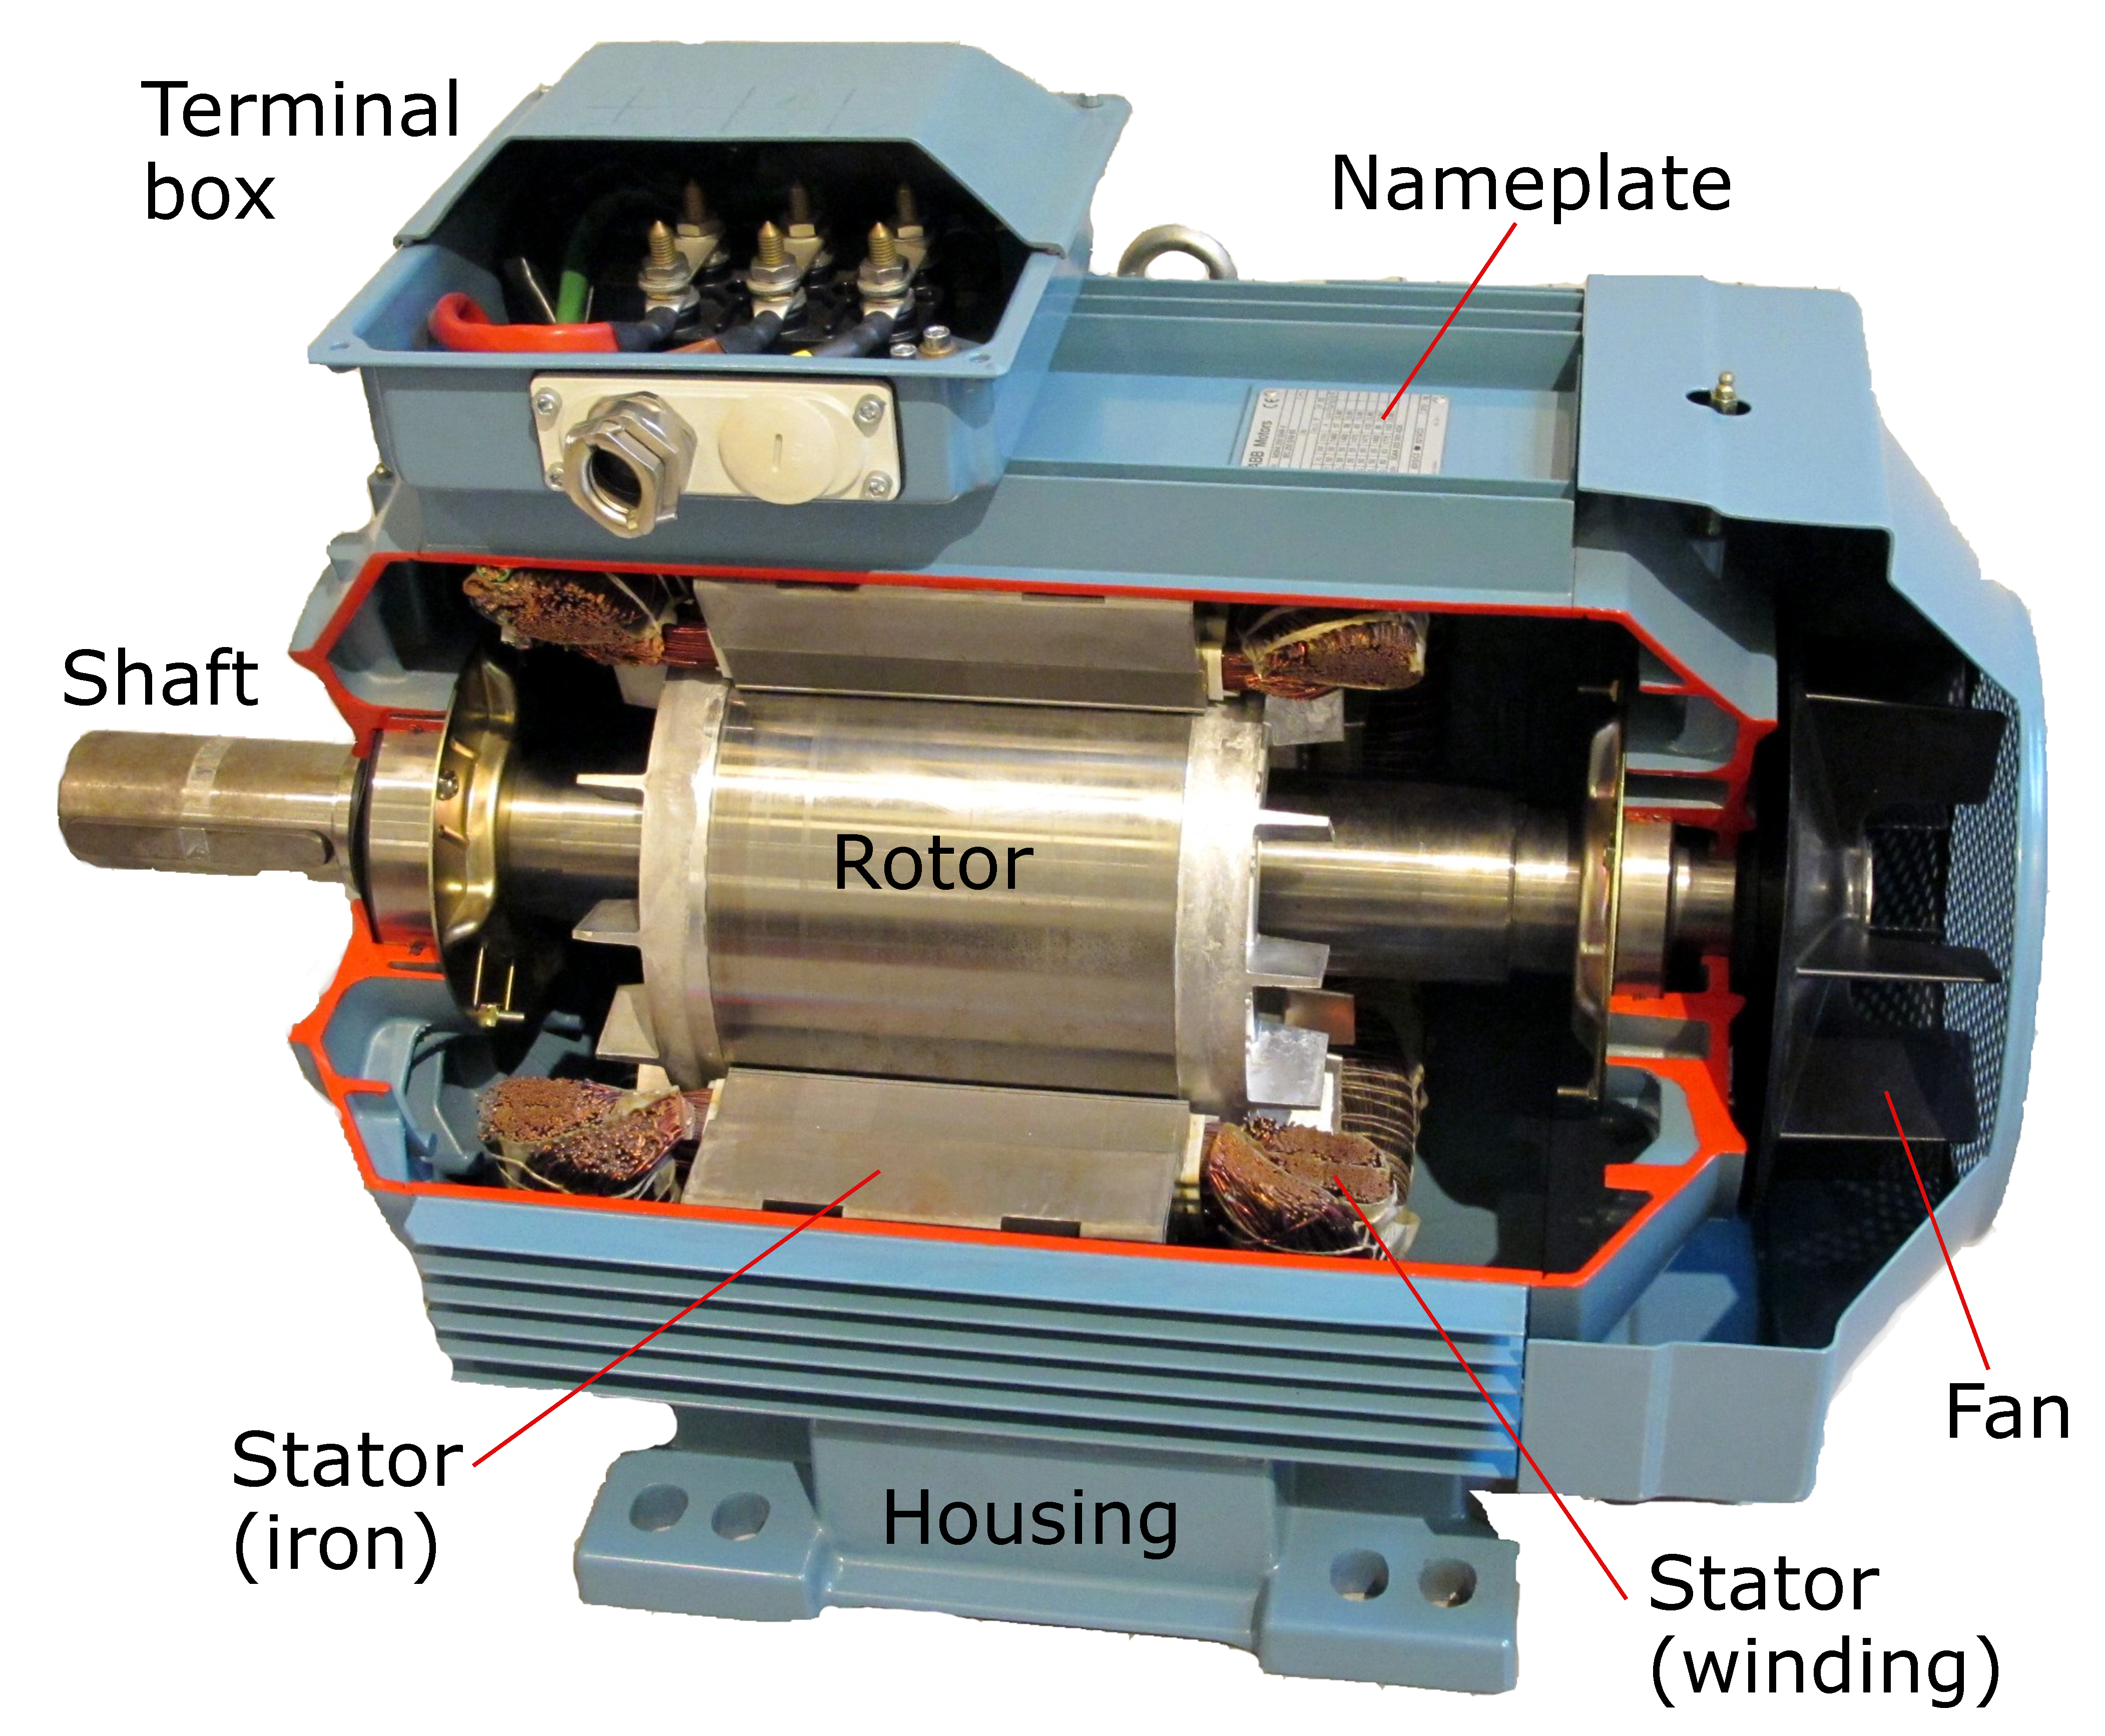
\includegraphics[width=0.95\textwidth]{fig/lec01/Induction_machine_opened.pdf}
				\caption{Example of an electrical machine (source: derived from \href{https://commons.wikimedia.org/wiki/File:TMW_50906_Schnittmodell_einer_Drehstrommaschine_(Asynchronmaschine).jpg}{Wikimedia Commons}, public domain)}
			\end{figure}
		\end{column}
		\end{columns}
\end{frame}

%%%%%%%%%%%%%%%%%%%%%%%%%%%%%%%%%%%%%%%%%%%%%%%%%%%%%%%%%%%%%
%% Some exemplary electrical machines %%
%%%%%%%%%%%%%%%%%%%%%%%%%%%%%%%%%%%%%%%%%%%%%%%%%%%%%%%%%%%%%
\begin{frame}
	\frametitle{Some exemplary electrical machines}
	\begin{figure}
		\centering
		\begin{subfigure}[b]{0.49\textwidth}
			\centering
			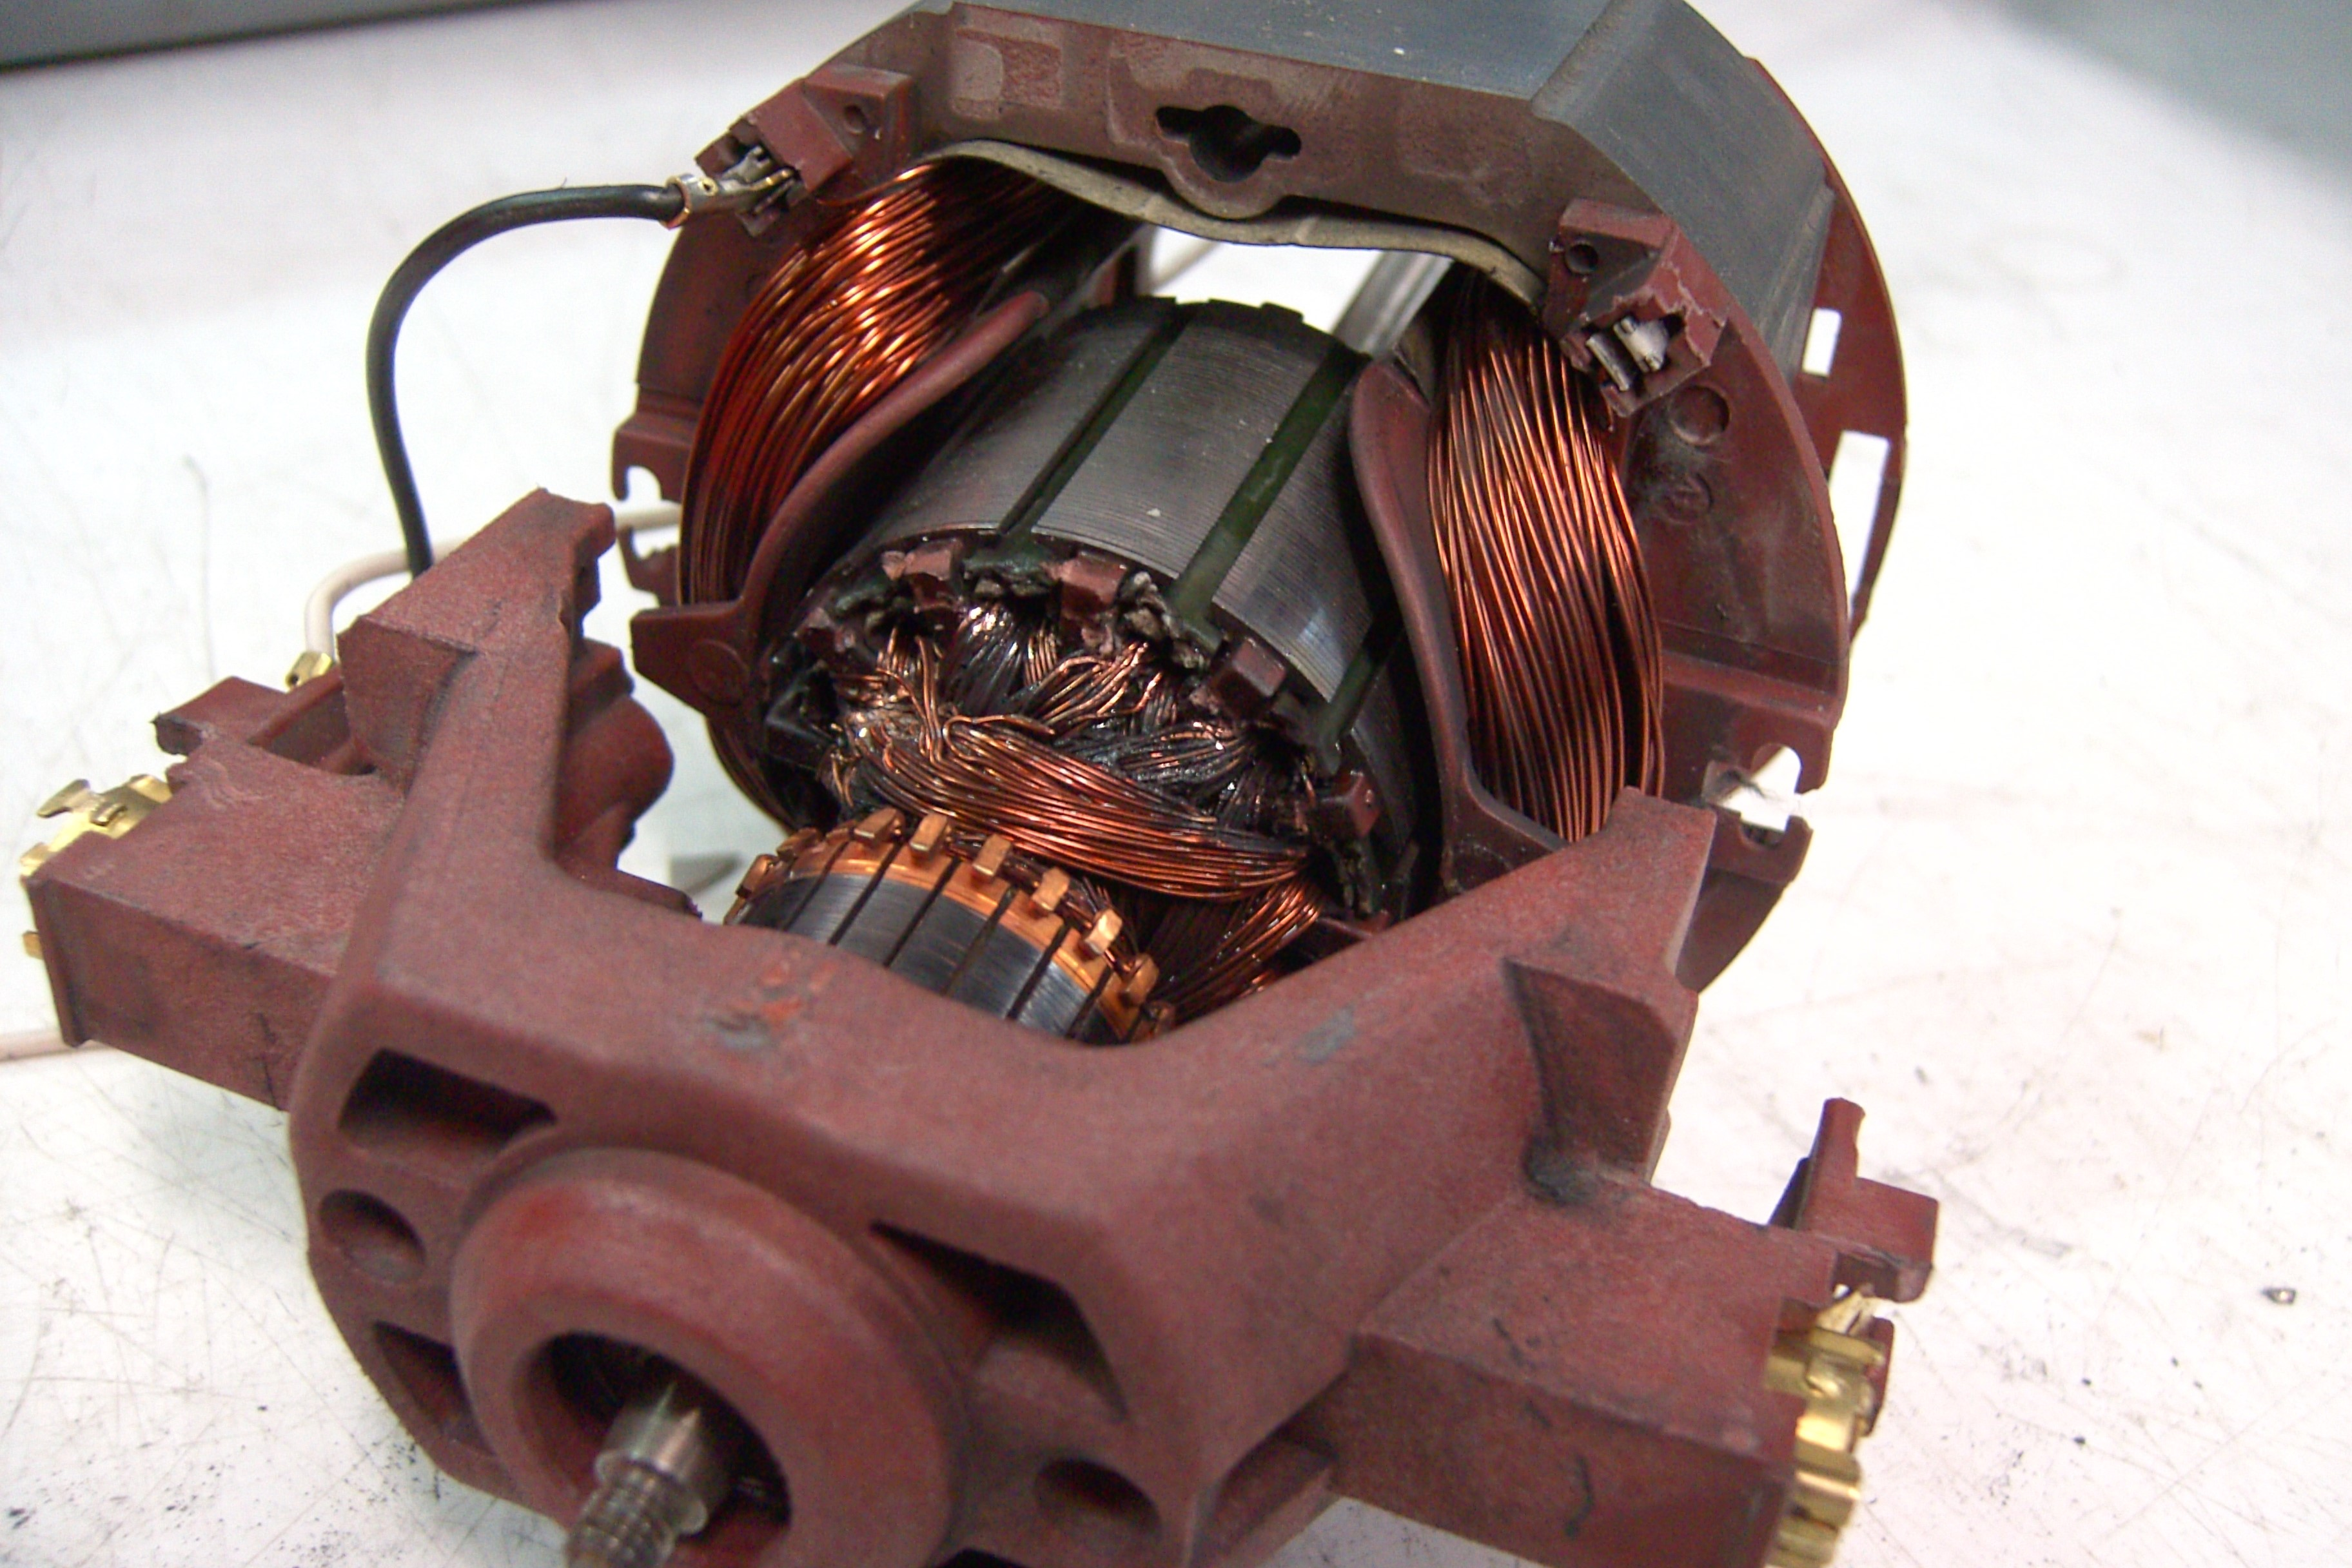
\includegraphics[width=0.5\textwidth]{fig/lec01/Universalmotor.JPG}
			\caption{DC machine (source: \href{https://commons.wikimedia.org/wiki/File:Universalmotor_3.JPG}{Wikimedia Commons}, Marrci, \href{https://creativecommons.org/licenses/by-sa/3.0/deed.en}{CC BY-SA 3.0})}
		\end{subfigure}
		\hfill
		\begin{subfigure}[b]{0.49\textwidth}
			\centering
			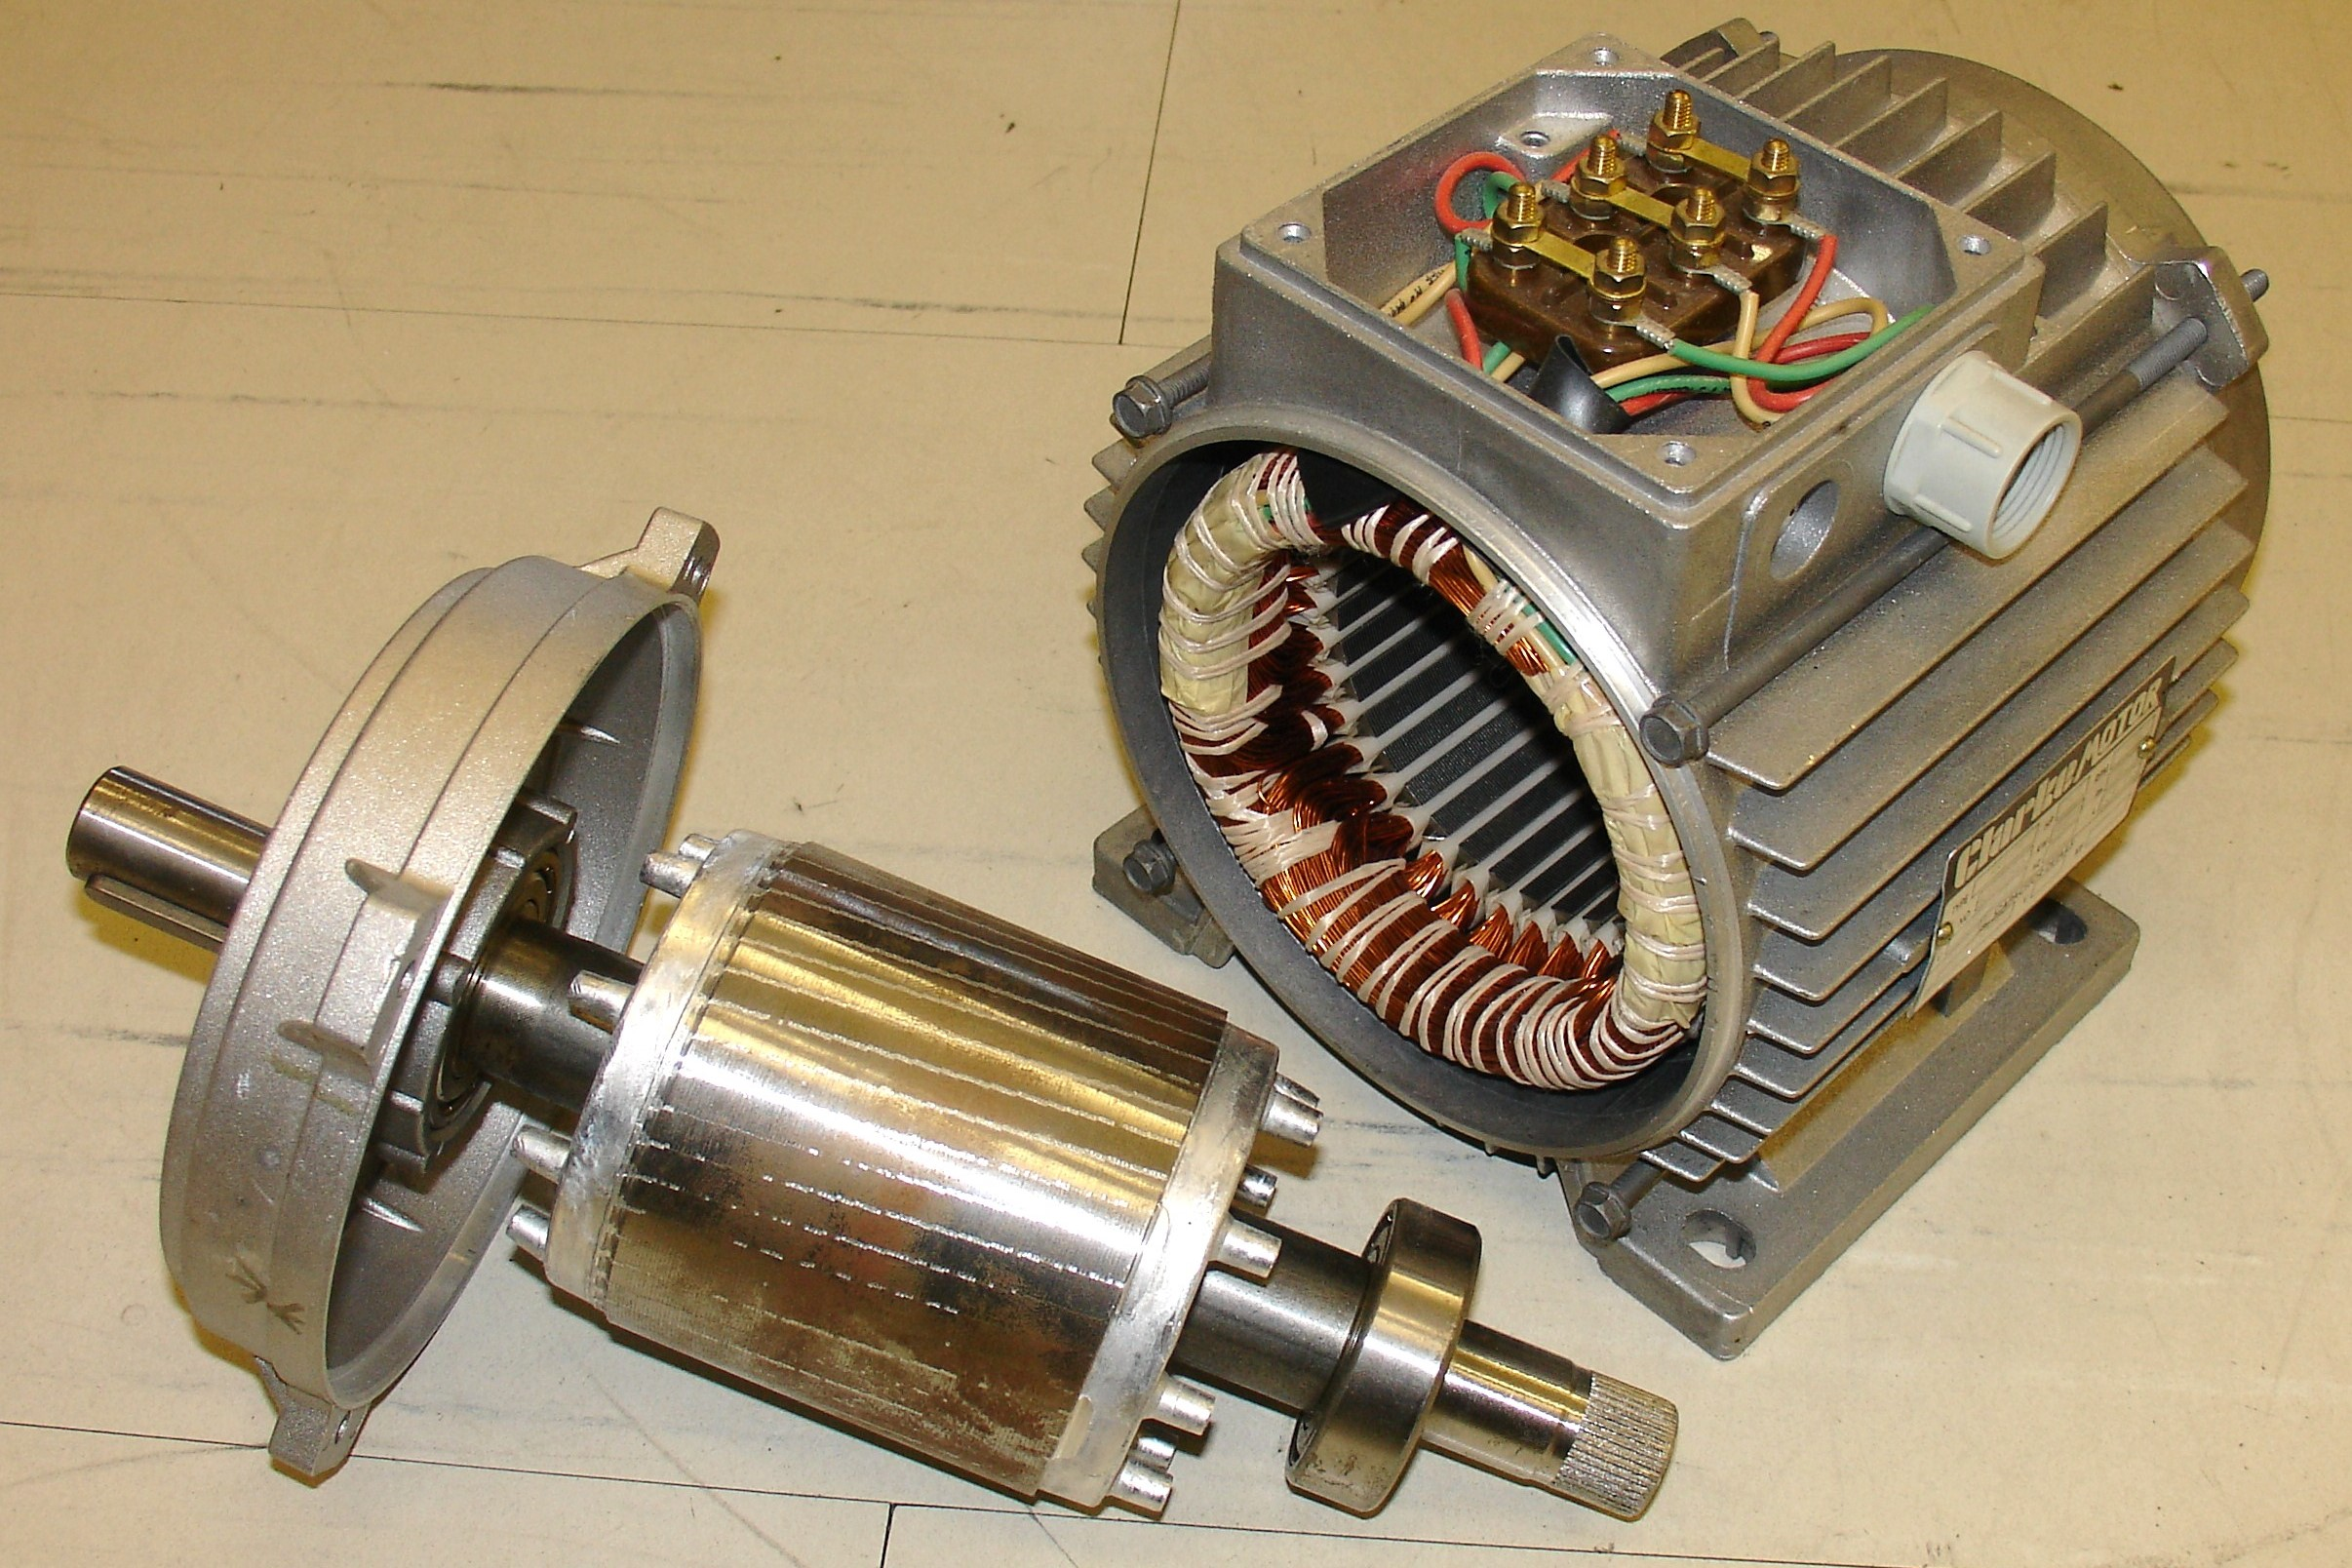
\includegraphics[width=0.5\textwidth]{fig/lec01/Induction_motor_stator_rotor.JPG}
			\caption{Induction machine (source: \href{https://commons.wikimedia.org/wiki/File:Stator_and_rotor_by_Zureks.JPG}{Wikimedia Commons}, Zureks, \href{https://creativecommons.org/licenses/by-sa/4.0/deed.en}{CC BY-SA 4.0})}
		\end{subfigure}
		\\
		\begin{subfigure}[b]{0.49\textwidth}
			\centering
			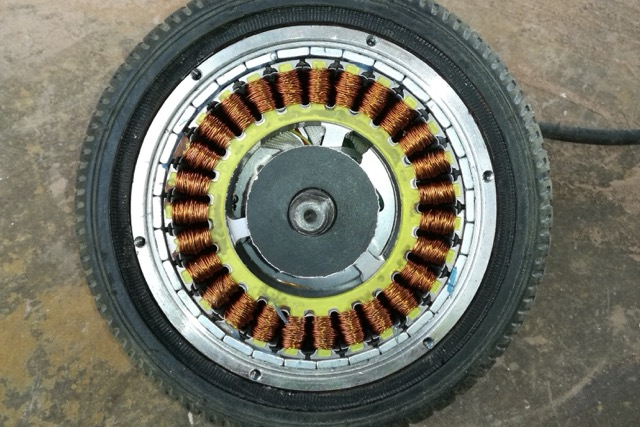
\includegraphics[width=0.5\textwidth]{fig/lec01/Wheel_hub_PMSM.jpg}
			\caption{Permanent magnet machine (source: \href{https://commons.wikimedia.org/wiki/File:Wheel_hub_motor_of_an_electric_kick_scooter,_sidepanel_removed_(2022).jpg}{Wikimedia Commons}, Andrez, \href{https://creativecommons.org/licenses/by-sa/4.0/deed.en}{CC BY-SA 4.0})}
		\end{subfigure}
		\hfill
		\begin{subfigure}[b]{0.49\textwidth}
			\centering
			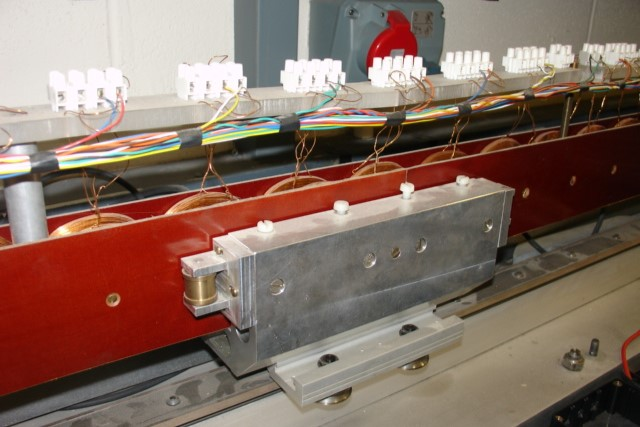
\includegraphics[width=0.5\textwidth]{fig/lec01/Linear_motor.jpg}
			\caption{Linear permanent magnet machine (source: \href{https://commons.wikimedia.org/wiki/File:Linear_motor_by_Zureks.jpg}{Wikimedia Commons}, Zureks, \href{https://creativecommons.org/licenses/by-sa/4.0/n}{CC BY-SA 4.0})}
		\end{subfigure}
		\caption*{Some exemplary electrical machines} 
        \label{fig:examples_machine_drives_00}
	\end{figure}
\end{frame}


%%%%%%%%%%%%%%%%%%%%%%%%%%%%%%%%%%%%%%%%%%%%%%%%%%%%%%%%%%%%%
%% The machine as an electrical-mechanical converter %%
%%%%%%%%%%%%%%%%%%%%%%%%%%%%%%%%%%%%%%%%%%%%%%%%%%%%%%%%%%%%%
\begin{frame}
	\frametitle{The machine as an electrical-mechanical converter}
	\begin{figure}
		\centering
		\begin{subfigure}[b]{0.49\textwidth}
			\centering
			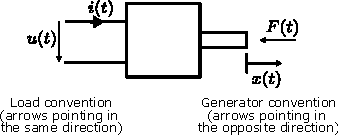
\includegraphics[width=0.9\textwidth]{fig/lec01/Block_diagram_translational_converter.pdf}
			\caption{Translational converter}
		\end{subfigure}
		\hfill
		\begin{subfigure}[b]{0.49\textwidth}
			\centering
			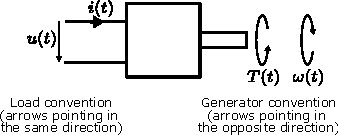
\includegraphics[width=0.9\textwidth]{fig/lec01/Block_diagram_rotational_converter.pdf}
			\caption{rotational converter}
		\end{subfigure}
		\caption{Electrically and mechanically free body diagrams of motors as energy converters  with variable notation: time $t$, voltage $u$, current $i$, force $F$, displacement $x$, torque $T$ and rational speed $\omega$ (adapted from J.~B\"ocker, \textit{Elektrische Antriebstechnik}, Paderborn University, 2020)} 
        \label{fig:free_body_diagrams_motor}
	\end{figure}
\end{frame}

%%%%%%%%%%%%%%%%%%%%%%%%%%%%%%%%%%%%%%%%%%%%%%%%%%%%%%%%%%%%%
%% Some basic mechanical terms (recap) %%
%%%%%%%%%%%%%%%%%%%%%%%%%%%%%%%%%%%%%%%%%%%%%%%%%%%%%%%%%%%%%
\begin{frame}
	\frametitle{Some basic mechanical terms (recap)}
	\vspace{-0.15cm}
	\begin{table}
		\centering
		\begin{tabular}{lll}
			& Translational converter & Rotational converter \\
			\toprule
			Kinematic quantities & & \\
			
			Displacement / angle & $x$ & $\varepsilon$ \\
			Velocity & $v=\dot{x}$ & $\omega=\dot{\varepsilon}$ \\
			Acceleration & $a=\dot{v}=\ddot{x}$ & $\alpha=\dot{\omega}=\ddot{\varepsilon}$ \\
			Jerk & $j=\dot{a}=\ddot{v}=\dddot{x}$ & $\rho=\dot{\alpha}=\ddot{\omega}=\dddot{\varepsilon}$ \\
			\midrule
			Dynamical quantities & & \\
			Force / torque & $F$ & $T$ \\
			Mass / inertia & $m$ & $J$ \\
			\midrule
			Mechanical power & $P_\mathrm{me}=F v$ & $P_\mathrm{me}=T \omega$ \\
			Work & $W[t_0,t]=\int_{t_0}^t P_\mathrm{me}(\tau)\,\mathrm{d}\tau$ & $W[t_0,t]=\int_{t_0}^t P_\mathrm{me}(\tau)\,\mathrm{d}\tau$ \\
			Momentum / rotational momentum & $p = m v$ & $L = \omega J$ \\
			Kinetic energy & $E_\mathrm{kin} = \frac{1}{2} m v^2$ & $E_\mathrm{kin} = \frac{1}{2} J \omega^2$ \\
			\bottomrule
		\end{tabular}
		\caption{Basic mechanical terms for translational and rotational converters}
		\label{tab:basic_mechanical_terms}
	\end{table}
\end{frame}

%%%%%%%%%%%%%%%%%%%%%%%%%%%%%%%%%%%%%%%%%%%%%%%%%%%%%%%%%%%%%
%% Work vs. energy (recap) %%
%%%%%%%%%%%%%%%%%%%%%%%%%%%%%%%%%%%%%%%%%%%%%%%%%%%%%%%%%%%%%
\begin{frame}
	\frametitle{Work vs. energy (recap)}
	\begin{columns}
		\begin{column}{0.5\textwidth}
			\begin{varblock}{Work}
				Work is the integral of the power over a time integral (or force over distance) and is a measure of the energy transfer.
			\end{varblock}
		\end{column}
		\begin{column}{0.5\textwidth}
			\begin{varblock}{Energy}
				Energy is the capacity to do work, that is, a quantity depending on the state of a system at a given point of time.				
			\end{varblock}
		\end{column}
		\end{columns}
		\vspace{0.5cm}
		\begin{figure}
			\centering
			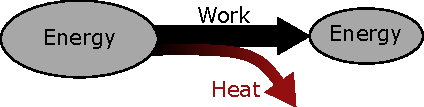
\includegraphics[width=0.6\textwidth]{fig/lec01/Work_Energy.pdf}
			\caption{Illustration addressing the work vs. energy terminology (simplified Sankey diagram)}
			\label{fig:work_vs_energy}
		\end{figure}
\end{frame}

%%%%%%%%%%%%%%%%%%%%%%%%%%%%%%%%%%%%%%%%%%%%%%%%%%%%%%%%%%%%%
%% Power balance of an electrical machine %%
%%%%%%%%%%%%%%%%%%%%%%%%%%%%%%%%%%%%%%%%%%%%%%%%%%%%%%%%%%%%%
\begin{frame}
	\frametitle{Power balance of an electrical machine}
	\begin{figure}
		\centering
		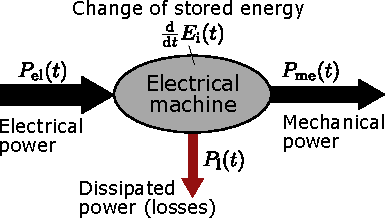
\includegraphics[width=0.45\textwidth]{fig/lec01/Power_balance_machine.pdf}
		\caption{Power balance of an electrical machine (illustrated in motoric operation)}
		\label{fig:power_balance_machine}
	\end{figure}
	The power balance
	\begin{equation}
		P_\mathrm{el}(t) = P_\mathrm{me}(t) + P_\mathrm{l}(t) + \frac{\mathrm{d}}{\mathrm{d}t}E_\mathrm{i}(t)
	\end{equation}
	must hold for any point in time as energy is conserved, that is, not created or destroyed.
\end{frame}

%%%%%%%%%%%%%%%%%%%%%%%%%%%%%%%%%%%%%%%%%%%%%%%%%%%%%%%%%%%%%
%% Four quadrants of machine operation %%
%%%%%%%%%%%%%%%%%%%%%%%%%%%%%%%%%%%%%%%%%%%%%%%%%%%%%%%%%%%%%
\begin{frame}
	\frametitle{Four quadrants of machine operation}
	\begin{columns}
		\begin{column}{0.5\textwidth}
			For the steady state ($\dot{E}_{\mathrm{i}}(t)=0$), we define the \hl{machine efficiency} as the ratio of the converted energy to the input energy:
			\begin{align}
				\eta_\mathrm{mot} &= \frac{P_{\mathrm{me}}}{P_{\mathrm{el}}} = 1- \frac{P_{\mathrm{l}}}{P_{\mathrm{el}}},\\[0.5em]
				\eta_\mathrm{gen} &= \frac{P_{\mathrm{el}}}{P_{\mathrm{me}}} = 1- \frac{P_{\mathrm{l}}}{P_{\mathrm{me}}}.
			\end{align}
			Hence, we need to consider in which \hl{quadrant} the machine operates as this will influence the power flow direction.
		\end{column}
		\begin{column}{0.5\textwidth}
			\begin{figure}
				\centering
				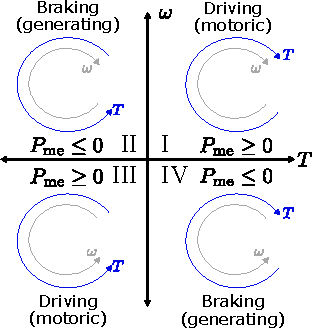
\includegraphics[width=0.75\textwidth]{fig/lec01/Machine_quadrants.pdf}
				\caption{Machine quadrants (derived from \href{https://de.wikipedia.org/wiki/Datei:Vierquadranten.svg}{Wikimedia Commons}, K. Pitter, \href{https://creativecommons.org/licenses/by-sa/3.0/deed.de}{CC BY-SA 3.0})}
			\end{figure}
		\end{column}
		\end{columns}
\end{frame}


%%%%%%%%%%%%%%%%%%%%%%%%%%%%%%%%%%%%%%%%%%%%%%%%%%%%%%%%%%%%%
%% What is an electrical drive ? %%
%%%%%%%%%%%%%%%%%%%%%%%%%%%%%%%%%%%%%%%%%%%%%%%%%%%%%%%%%%%%%
\begin{frame}
	\frametitle{What is an electrical drive ?}
	\begin{columns}
		\begin{column}{0.4\textwidth}
			\begin{varblock}{Electrical drive}
			   An electrical drive is a system that controls the torque, speed or position of an electrical machine connected to some mechanical process.
			\end{varblock}
			\vspace{0.25cm}
			\begin{itemize}
				\item Integrates the 'stupid' electrical machine into an 'intelligent' controlled system.
				\item The energy source and mechanical process ('load') are not part of the drive system.
			\end{itemize}
		\end{column}
		\begin{column}{0.6\textwidth}
			\begin{figure}
				\centering
				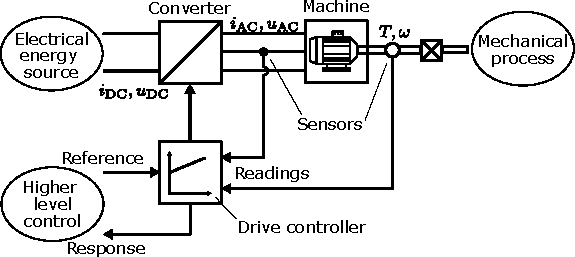
\includegraphics[width=0.95\textwidth]{fig/lec01/Electrical_Drive_Block_Overview.pdf}
				\caption{Block diagram of an electrical drive (adapted from J.~B\"ocker, \textit{Elektrische Antriebstechnik}, Paderborn University, 2020)}
			\end{figure}
		\end{column}
	\end{columns}
\end{frame}

%%%%%%%%%%%%%%%%%%%%%%%%%%%%%%%%%%%%%%%%%%%%%%%%%%%%%%%%%%%%%
%% Examples of electrical machine and drive applications (1) %%
%%%%%%%%%%%%%%%%%%%%%%%%%%%%%%%%%%%%%%%%%%%%%%%%%%%%%%%%%%%%%
\begin{frame}
	\frametitle{Examples of electrical machine and drive applications (1)}
	\begin{figure}
		\centering
		\begin{subfigure}[b]{0.49\textwidth}
			\centering
			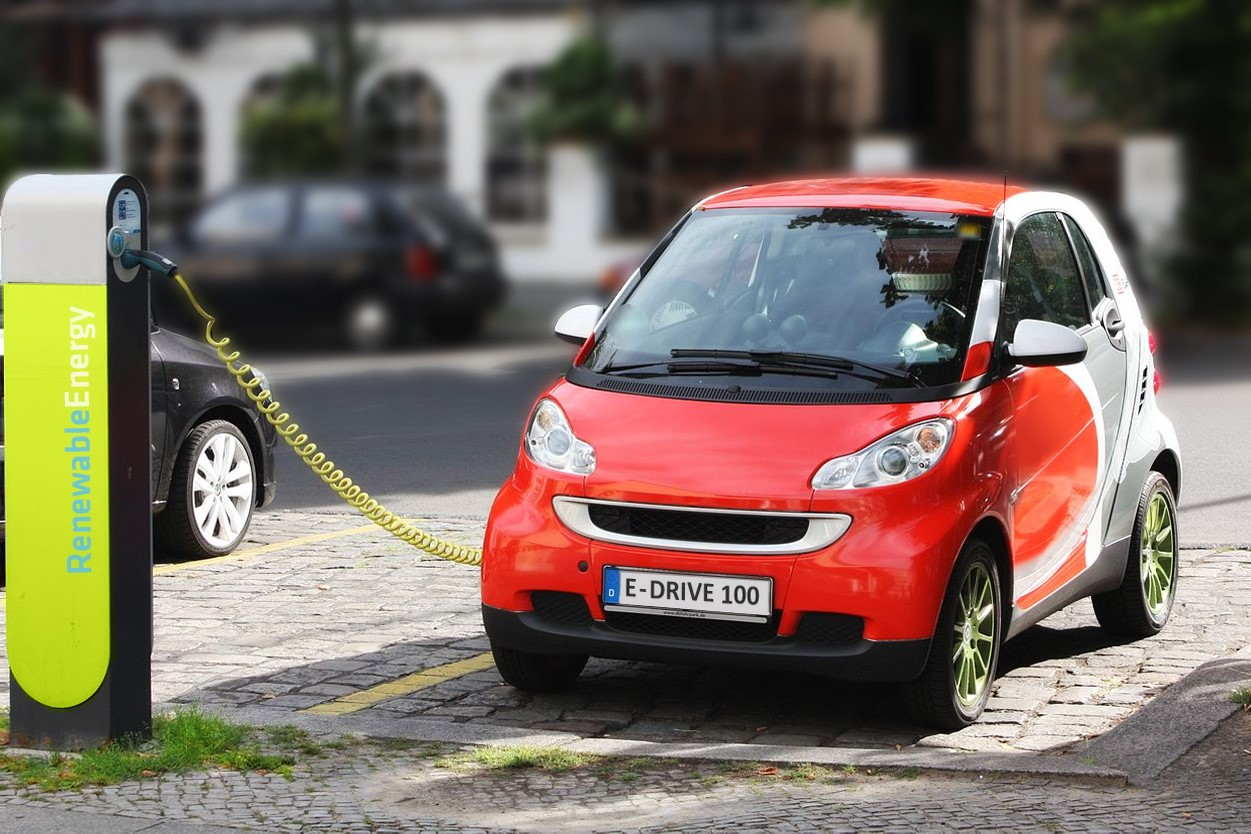
\includegraphics[width=0.5\textwidth]{fig/lec01/Electric_Car_recharging.jpg}
			\caption{Electric cars (source: \href{https://commons.wikimedia.org/wiki/File:Electric_Car_recharging.jpg}{Wikimedia Commons}, M.~Movchin and F. Mueller, \href{https://creativecommons.org/licenses/by-sa/3.0/deed.en}{CC BY-SA 3.0})}
		\end{subfigure}
		\hfill
		\begin{subfigure}[b]{0.49\textwidth}
			\centering
			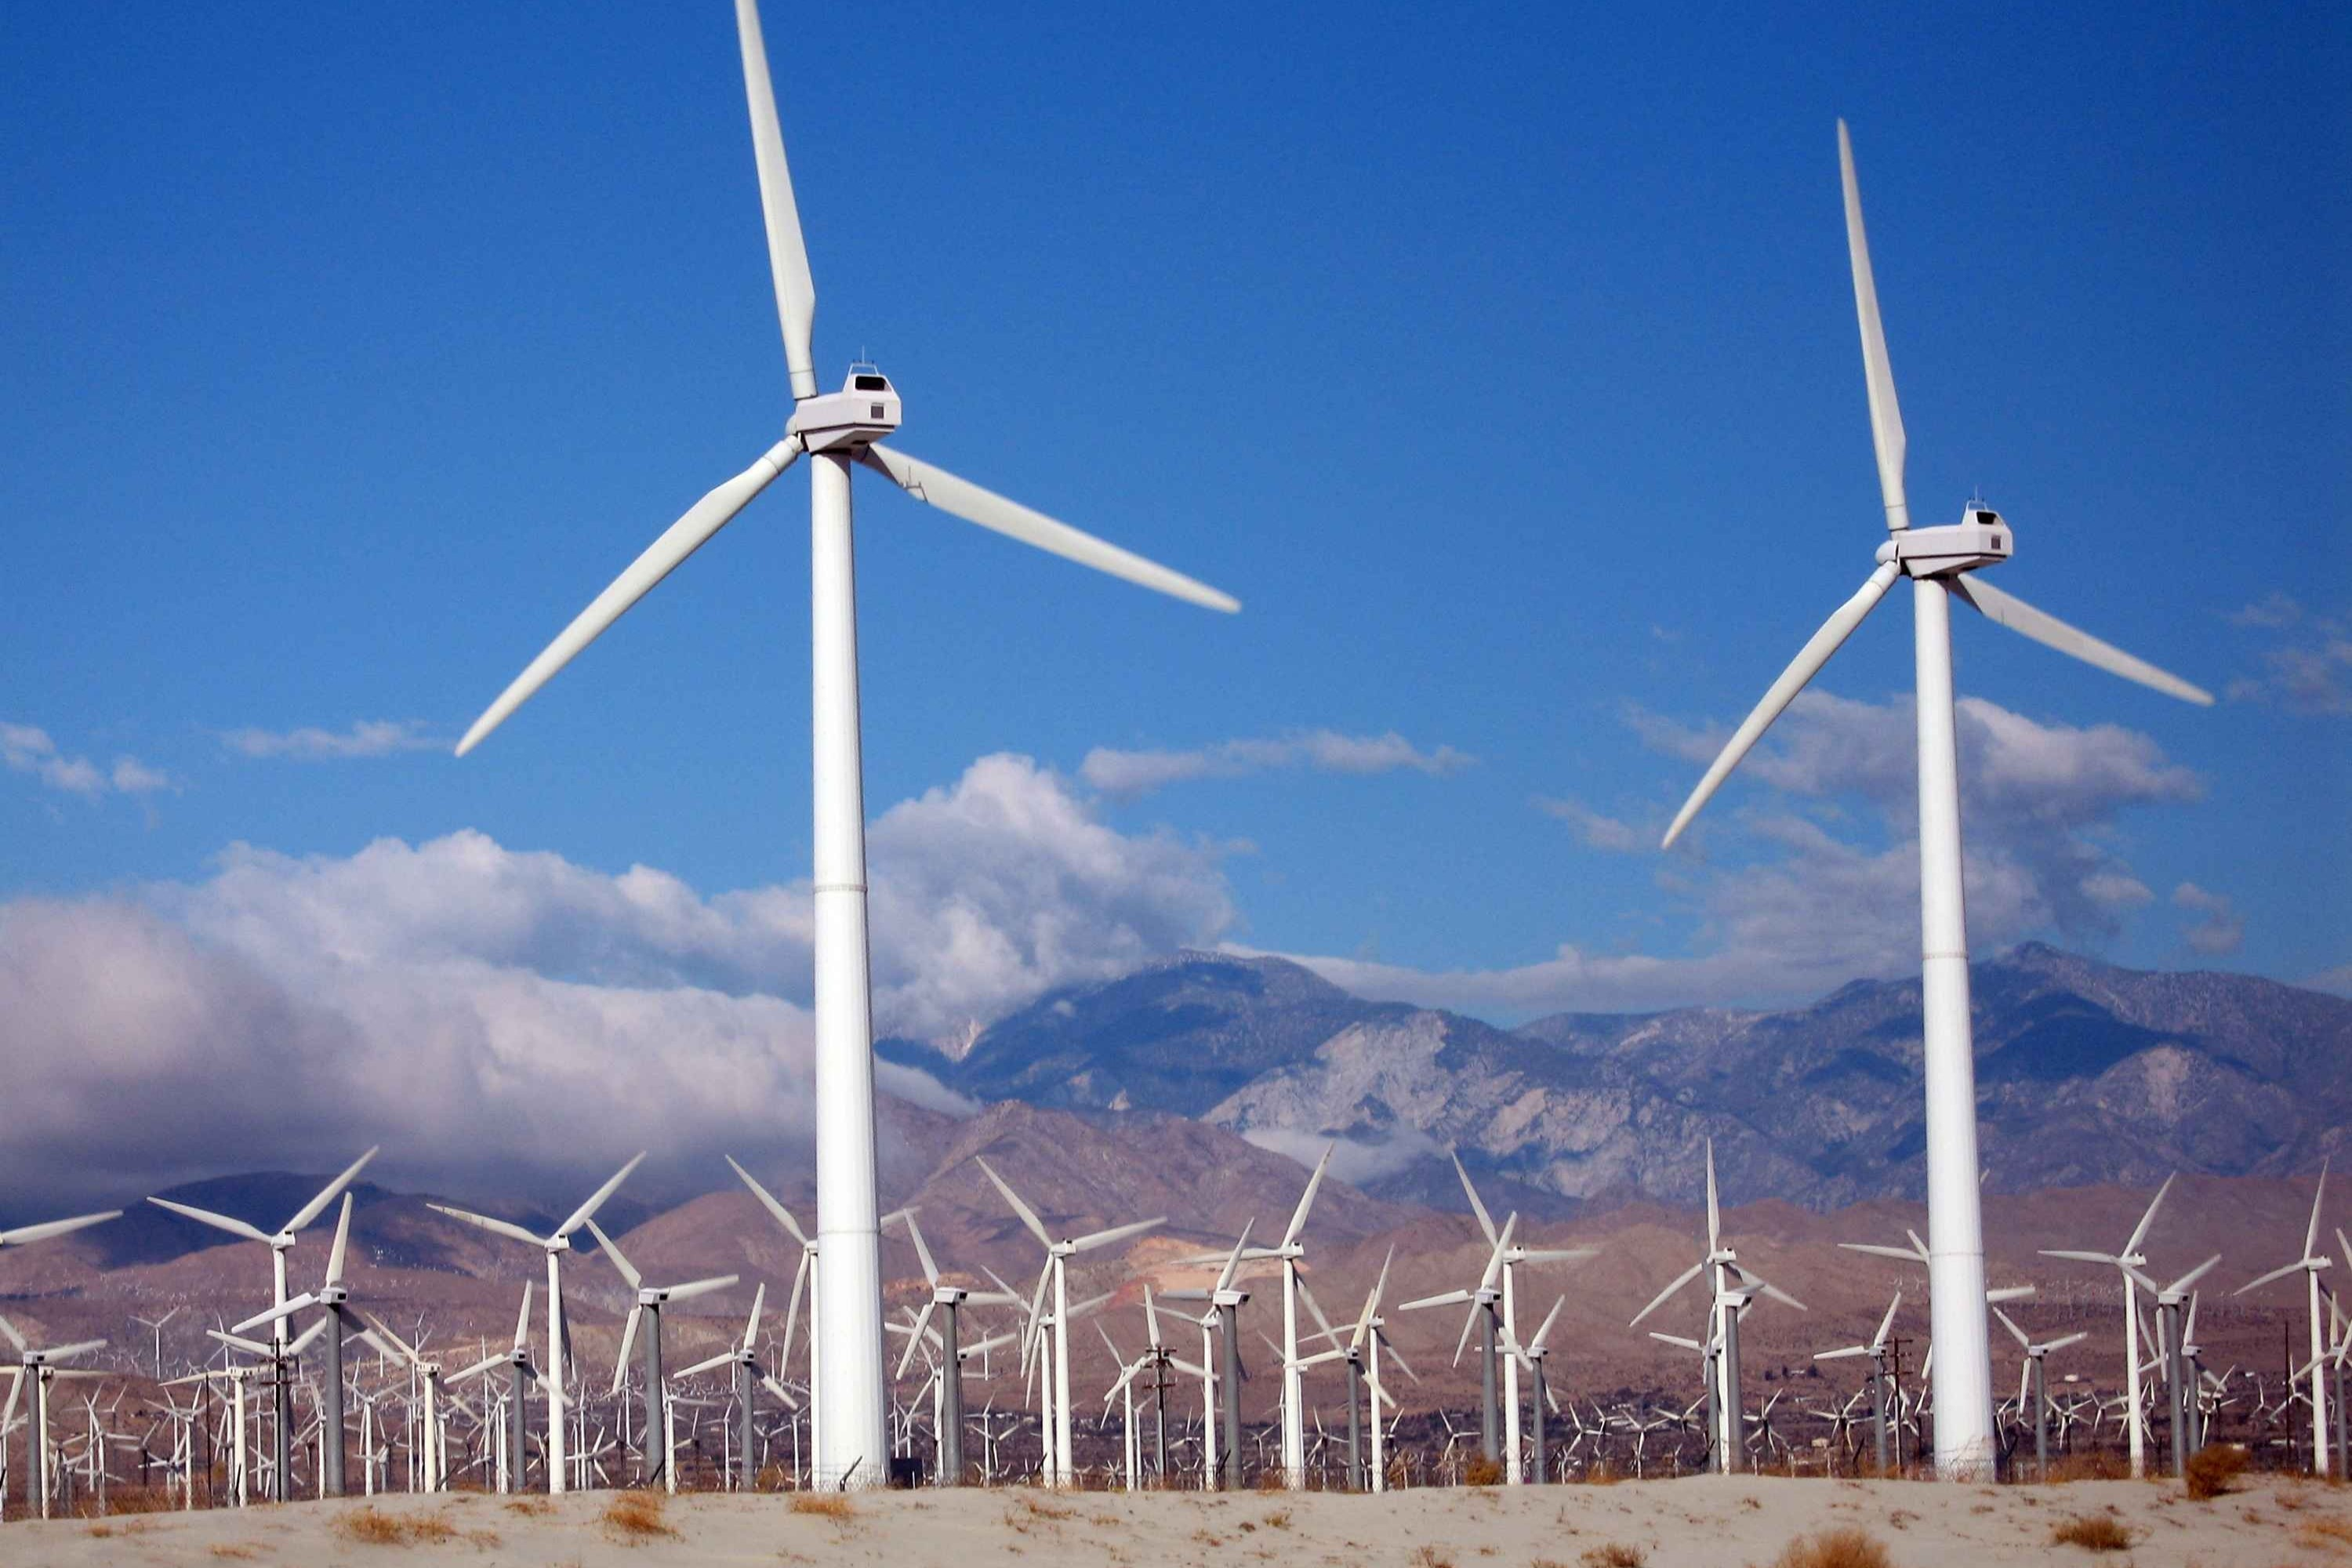
\includegraphics[width=0.5\textwidth]{fig/lec01/sky-farm-windmill.jpg}
			\caption{Wind turbine generators (source: \href{https://pxhere.com/en/photo/954757}{pxhere.com}, public domain)}
		\end{subfigure}
		\\
		\begin{subfigure}[b]{0.49\textwidth}
			\centering
			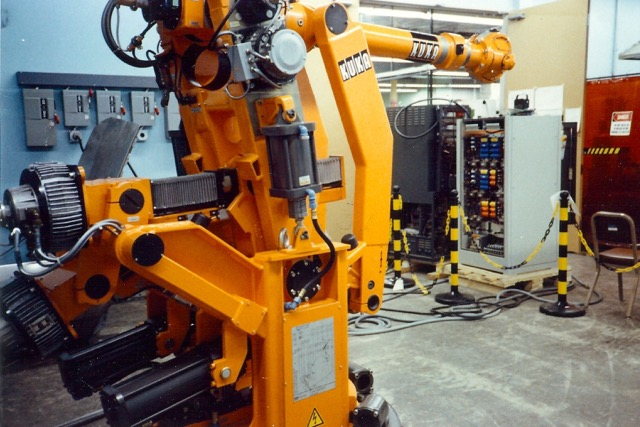
\includegraphics[width=0.5\textwidth]{fig/lec01/Automatix_KukaRobot.jpg}
			\caption{Factory robots (source: \href{https://commons.wikimedia.org/wiki/File:Automatix_KukaRobot483.agr.jpg}{Wikimedia Commons}, A.~Reinhold, \href{https://creativecommons.org/licenses/by-sa/4.0/deed.en}{CC BY-SA 4.0})}
		\end{subfigure}
		\hfill
		\begin{subfigure}[b]{0.49\textwidth}
			\centering
			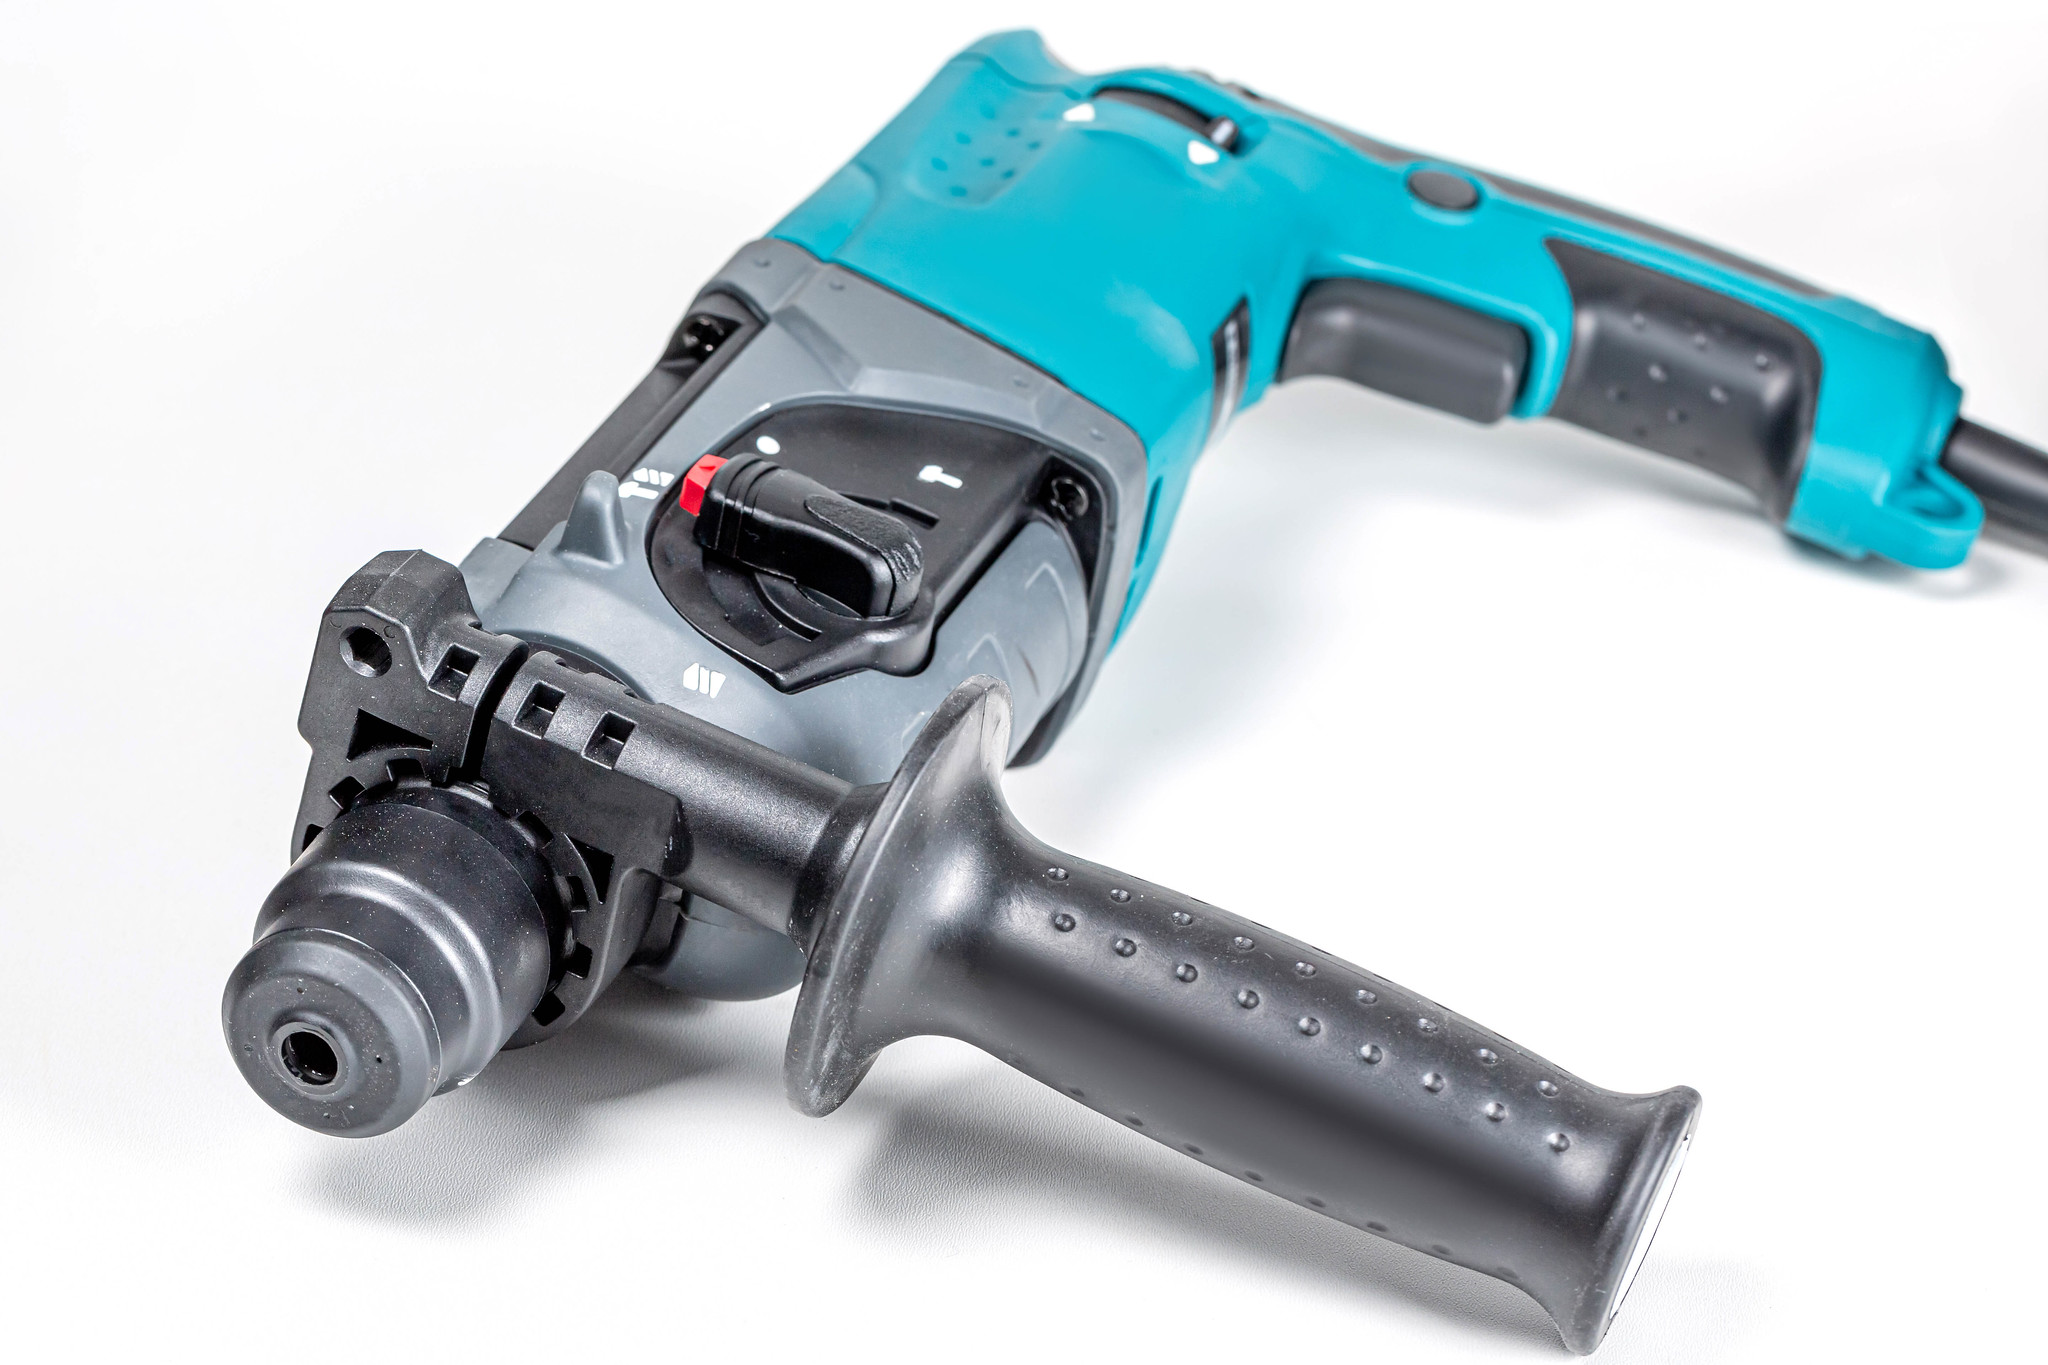
\includegraphics[width=0.5\textwidth]{fig/lec01/electric_drill.jpg}
			\caption{Electric tools (source: \href{https://www.flickr.com/photos/30478819@N08/49940384798}{flickr.com},  M.~Verch, \href{https://creativecommons.org/licenses/by/2.0/}{CC BY 2.0})}
		\end{subfigure}
		\caption*{Examples of electrical machine and drive applications} 
        \label{fig:examples_machine_drives_01}
	\end{figure}
\end{frame}

%%%%%%%%%%%%%%%%%%%%%%%%%%%%%%%%%%%%%%%%%%%%%%%%%%%%%%%%%%%%%
%% Examples of electrical machine and drive applications (2) %%
%%%%%%%%%%%%%%%%%%%%%%%%%%%%%%%%%%%%%%%%%%%%%%%%%%%%%%%%%%%%%
\begin{frame}
	\frametitle{Examples of electrical machine and drive applications (2)}
	% Set up a 2x2 grid of figures
	\begin{figure}
		\ContinuedFloat
		\centering
		\begin{subfigure}[b]{0.49\textwidth}
			\centering
			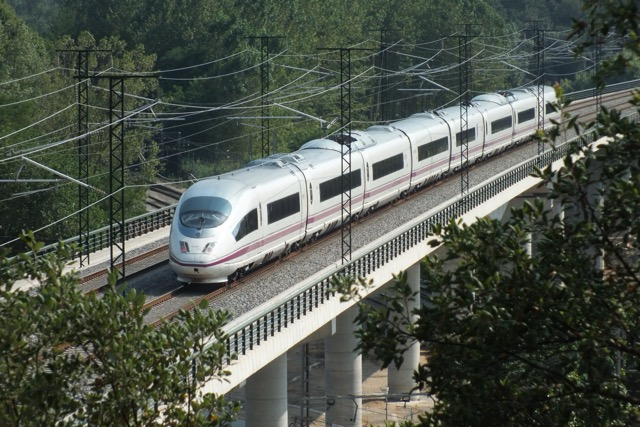
\includegraphics[width=0.5\textwidth]{fig/lec01/Train.jpg}
			\caption{High-speed trains (source: \href{https://commons.wikimedia.org/wiki/File:Fast_Train_Spain_Class_103_AVE_Siemens_Bridge_Macanet-Massanes.JPG}{Wikimedia Commons}, P.~Elektro, \href{https://creativecommons.org/licenses/by-sa/3.0/deed.en}{CC BY-SA 3.0})}
		\end{subfigure}
		\hfill
		\begin{subfigure}[b]{0.49\textwidth}
			\centering
			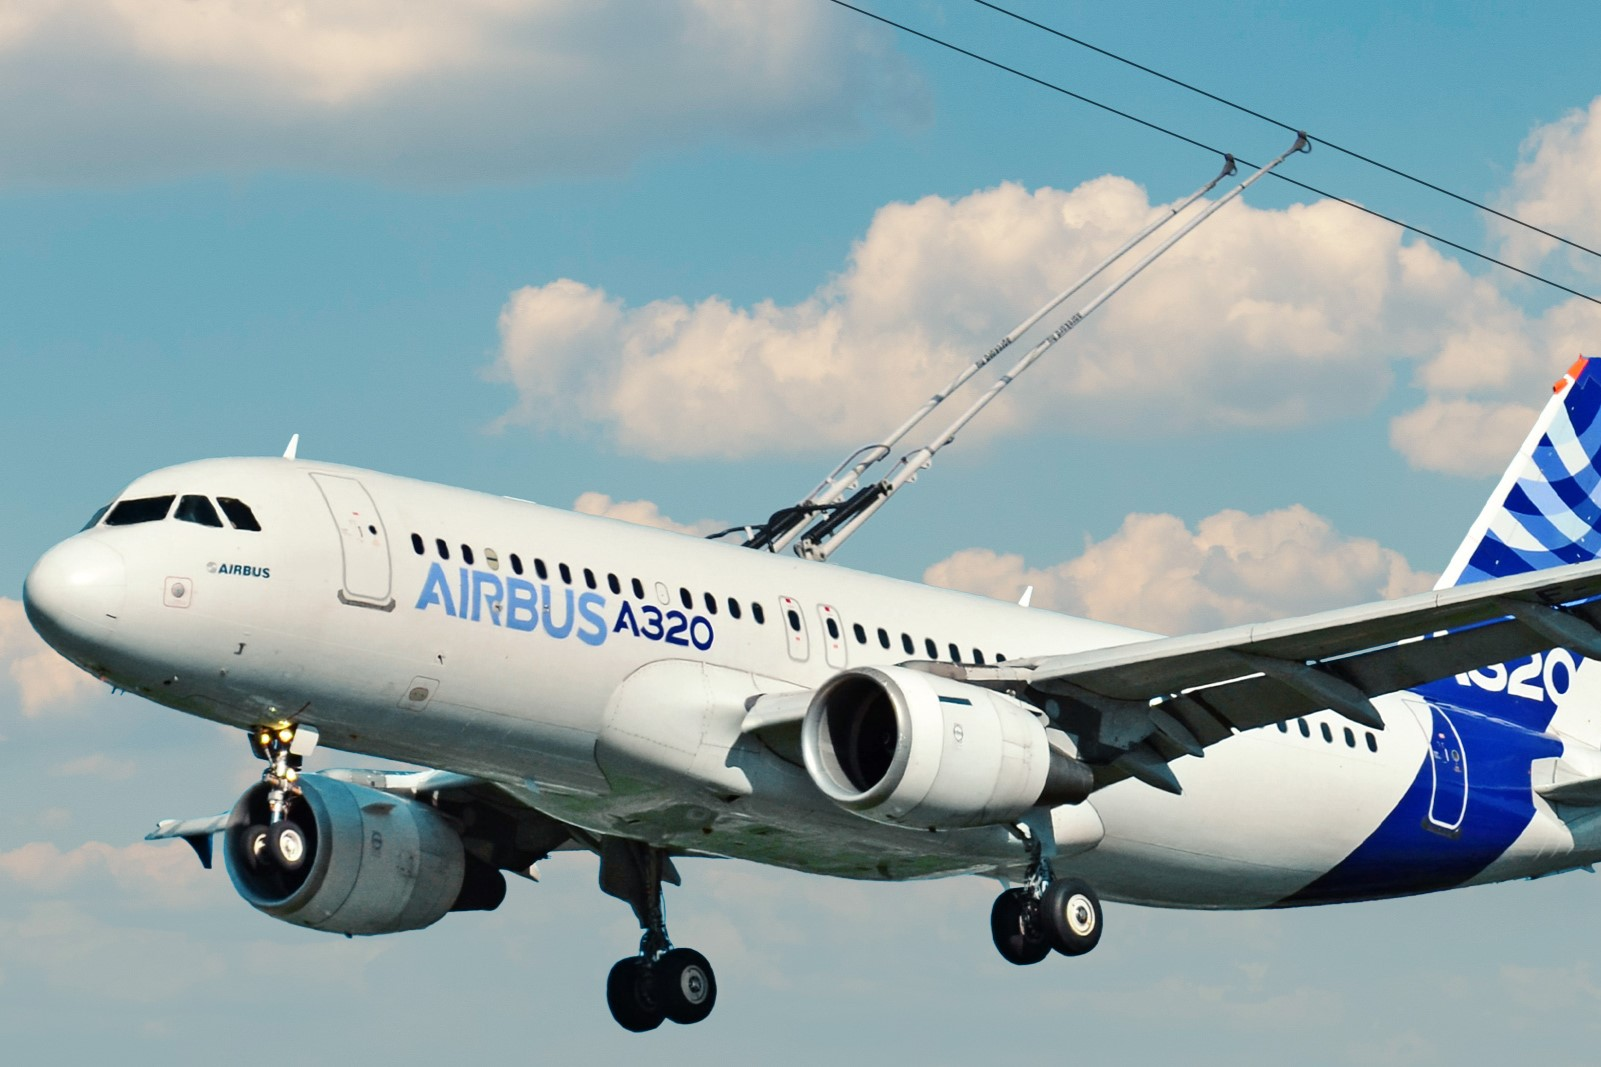
\includegraphics[width=0.5\textwidth]{fig/lec01/Electric_Airbus_A320.jpg}
			\caption{Electric aircrafts (source: \href{https://commons.wikimedia.org/wiki/File:Electric_Airbus_A320.jpg}{Wikimedia Commons}, M.~Weinold, \href{https://creativecommons.org/licenses/by-sa/4.0/deed.en}{CC BY-SA 4.0})}
		\end{subfigure}
		\\
		\begin{subfigure}[b]{0.49\textwidth}
			\centering
			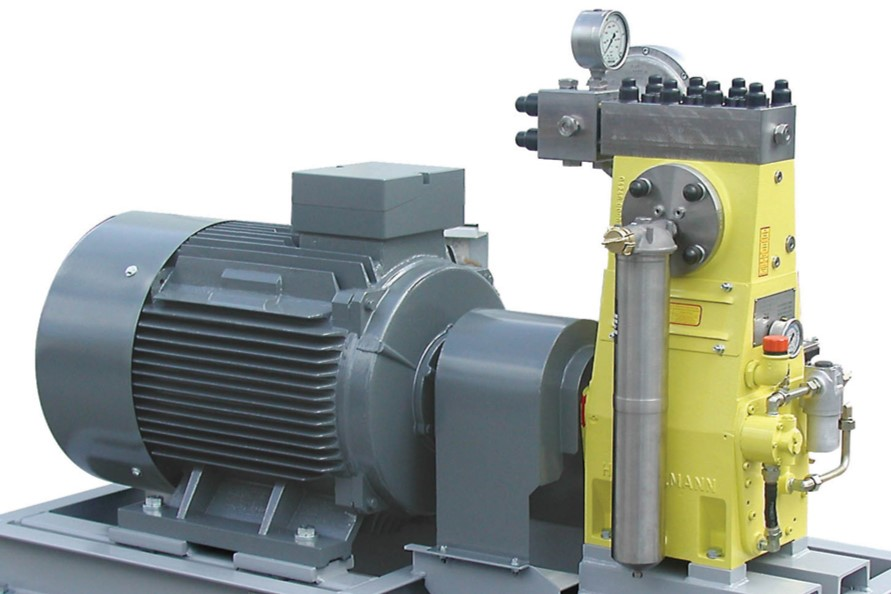
\includegraphics[width=0.5\textwidth]{fig/lec01/Pump.jpg}
			\caption{Pumps (source: \href{https://commons.wikimedia.org/wiki/File:Hammelmann_Stationary_unit_with_electric_motor.jpg}{Wikimedia Commons}, Hammelmann, \href{https://creativecommons.org/licenses/by-sa/3.0/deed.en}{CC BY-SA 3.0})}
		\end{subfigure}
		\hfill
		\begin{subfigure}[b]{0.49\textwidth}
			\centering
			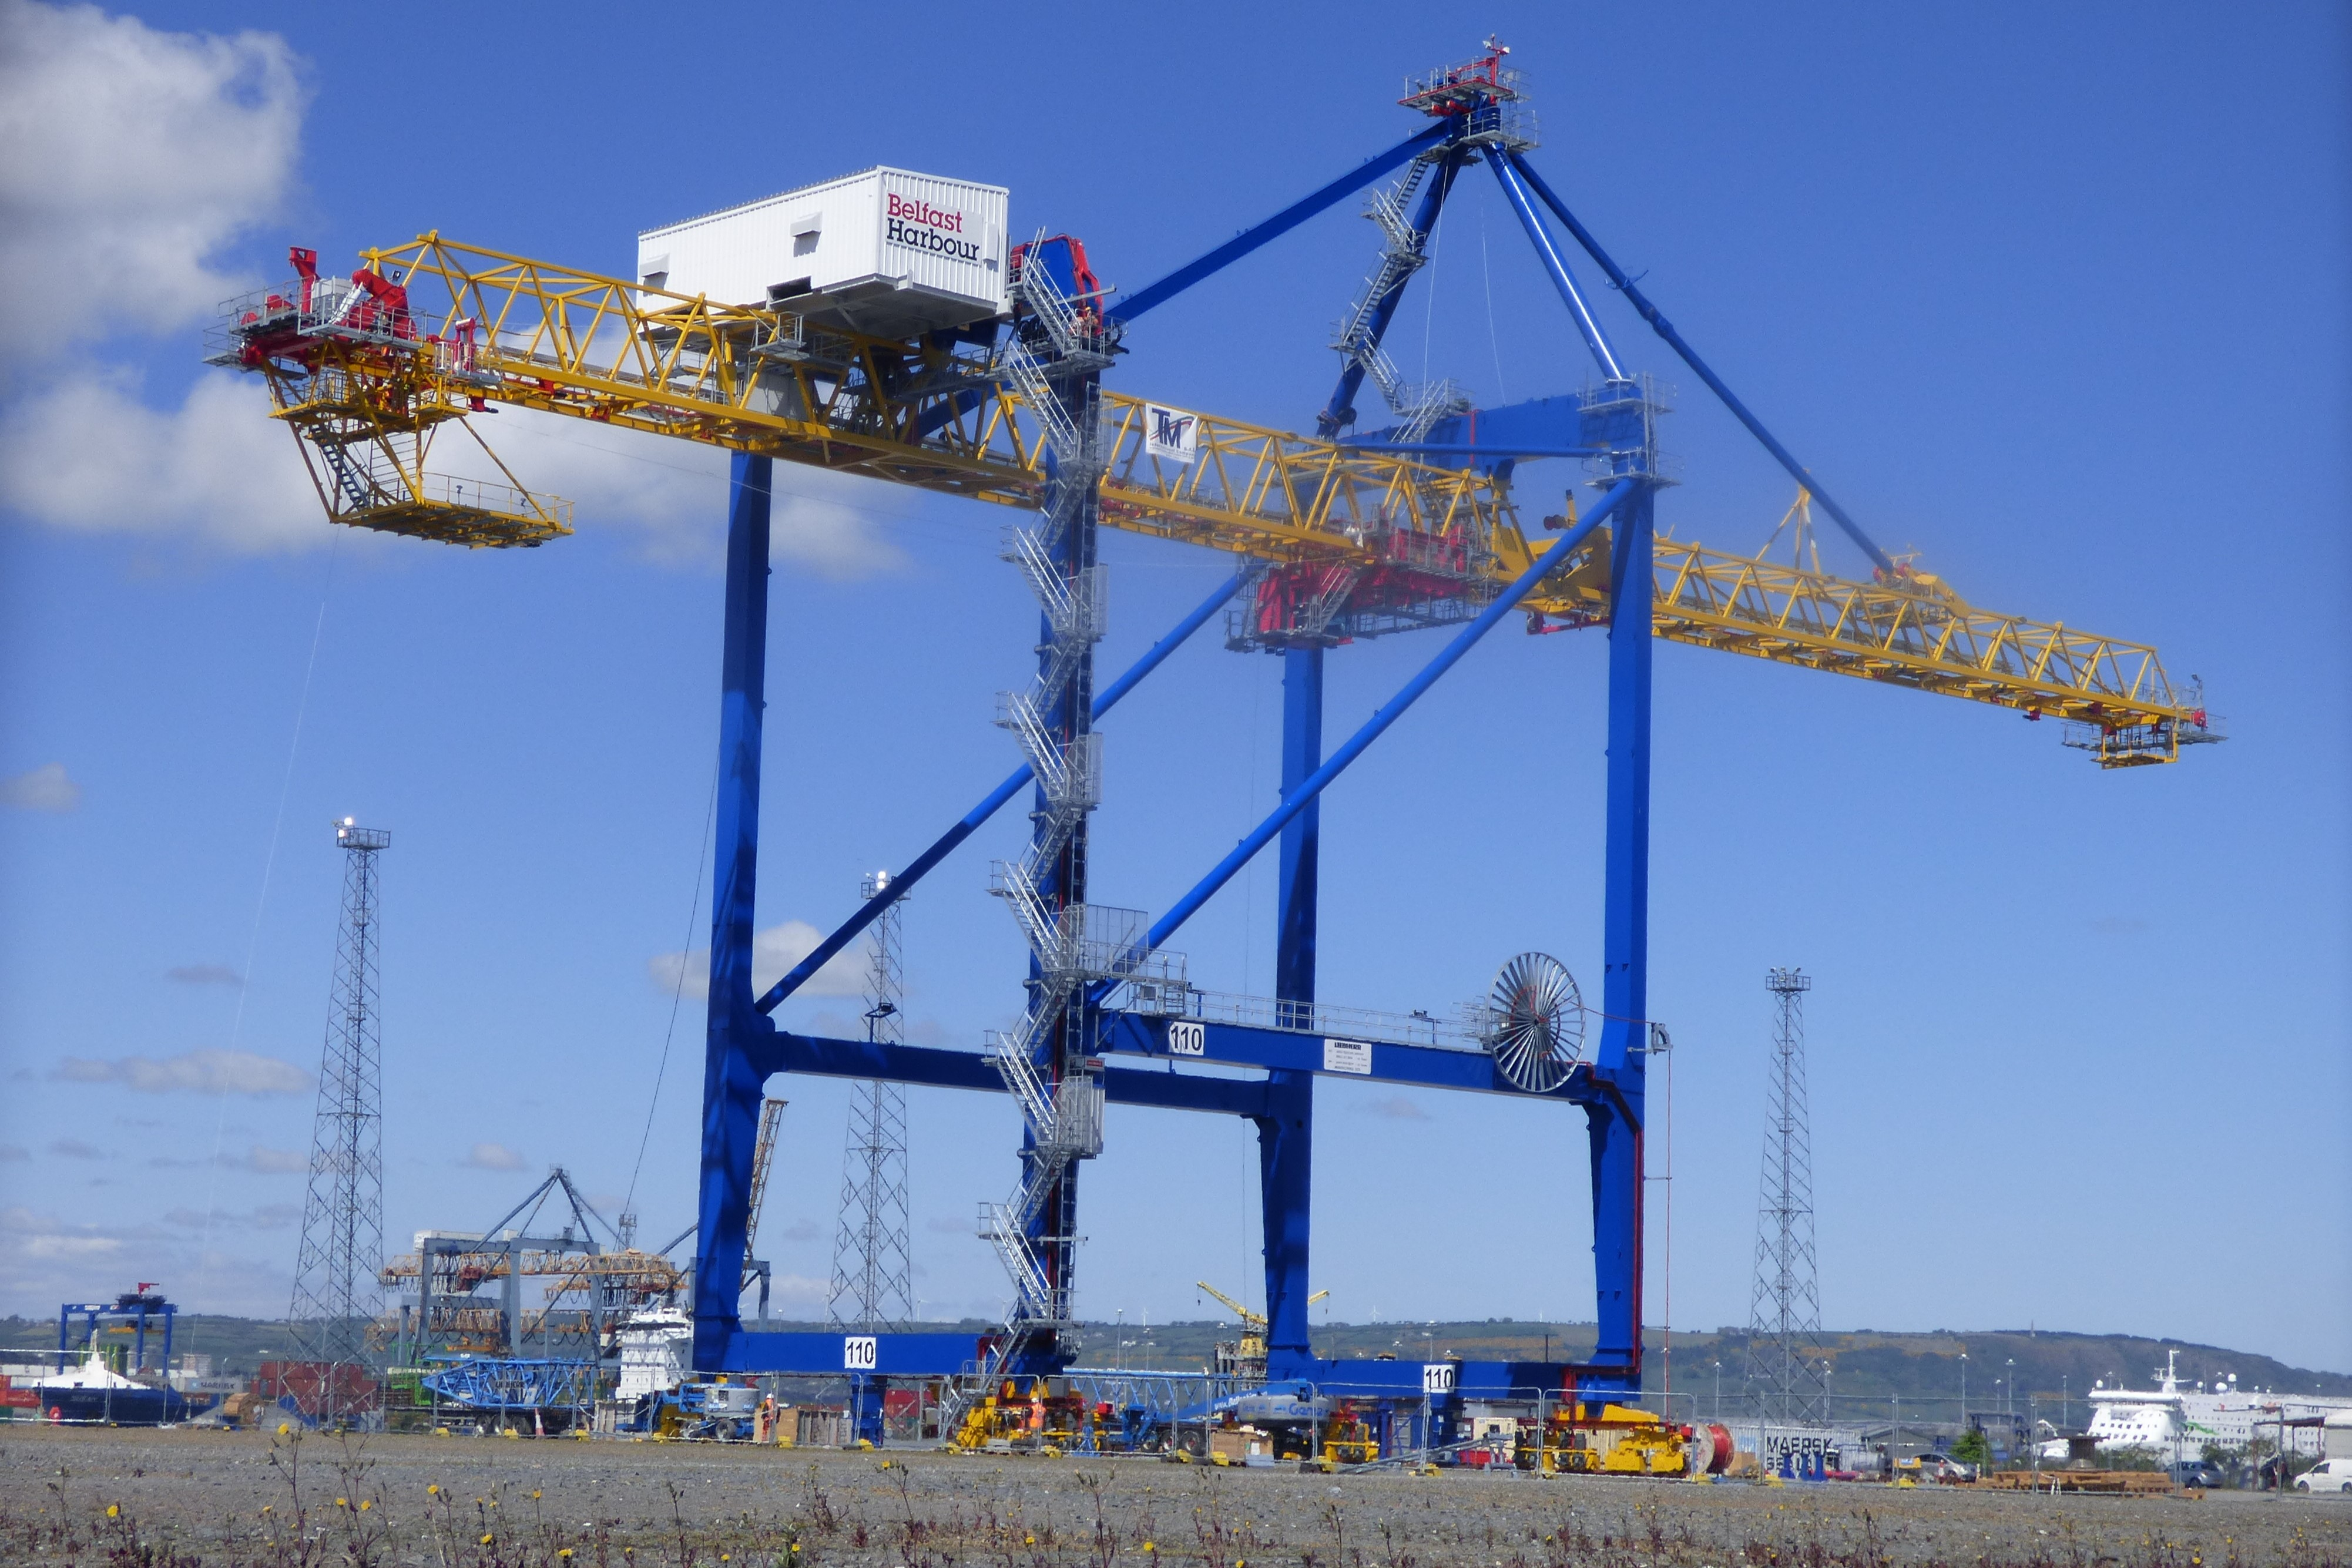
\includegraphics[width=0.5\textwidth]{fig/lec01/crane.jpg}
			\caption{Cranes (source: \href{https://commons.wikimedia.org/wiki/File:Hammelmann_Stationary_unit_with_electric_motor.jpg}{Wikimedia Commons}, Belfast Dissenter, \href{https://creativecommons.org/licenses/by-sa/4.0/deed.en}{CC BY-SA 4.0})}
		\end{subfigure}
		\caption*{Examples of electrical machine and drive applications} 
        \label{fig:examples_machine_drives_02}
	\end{figure}
\end{frame}

%%%%%%%%%%%%%%%%%%%%%%%%%%%%%%%%%%%%%%%%%%%%%%%%%%%%%%%%%%%%%
%% Examples of electrical machine and drive applications (2) %%
%%%%%%%%%%%%%%%%%%%%%%%%%%%%%%%%%%%%%%%%%%%%%%%%%%%%%%%%%%%%%
\begin{frame}
	\frametitle{A broad range of nominal power ratings}
	\vspace{-0.1cm}
	\begin{figure}
		\centering
		\includegraphics[height=0.7\textheight]{fig/lec01/Power_Classes_Examples.pdf}
		\caption{Power range overview (inspired  from A.~Binder, \textit{Elektrische Maschinen und Antriebe}, Darmstadt University, 2022 with additional figure sources: \href{https://www.flickr.com/photos/arthurwolf/5393520058/}{A. Wolf}, \href{https://commons.wikimedia.org/wiki/File:Wald_am_Arlberg-OeBB_Spullersee_power_plant-M1-Rotor-11ASD.jpg}{Asurnipal}, \href{https://www.flickr.com/photos/mouser-nerdbot/7042785635}{M. Williams}, \href{https://de.m.wikipedia.org/wiki/Datei:Stick_blender_Electrolux_AEG_HB_9807_-_stator_of_the_electric_motor-4313.jpg}{R. Spekking}, \href{https://commons.wikimedia.org/wiki/File:Electric_motor_and_transmission_in_a_truck.jpg}{Foxcorner}, \href{https://commons.wikimedia.org/wiki/File:E-bike_electric_motor_shimano_ep_8.jpg}{A.~Tredz} and \href{https://commons.wikimedia.org/wiki/File:2023_Corsair_SP120_RGB_Elite.jpg}{J. Halicki} under varying CC licenses) }
		\label{Power_Classes_Examples}
	\end{figure}
\end{frame}

%%%%%%%%%%%%%%%%%%%%%%%%%%%%%%%%%%%%%%%%%%%%%%%%%%%%%%%%%%%%%
%% Why are electric machines and drives important ? %%
%%%%%%%%%%%%%%%%%%%%%%%%%%%%%%%%%%%%%%%%%%%%%%%%%%%%%%%%%%%%%
\begin{frame}
	\frametitle{Why is knowledge about electric machines and drives important?}
	\begin{varblock}{Electric machines and drives are an essential pillar of the modern society}
		Without electric machines and drives, our todays' society would not be possible. Starting from providing electricity via electrical generators to powering electric vehicles, tools and entire factory production lines, electric machines and drives are everywhere, that is, they enable our today's living standard. 
	\end{varblock}
	\begin{varblock}{Energy efficiency and sustainability is key}
		Electric machines and drives utilize  approx. 50\,\% of the global electricity with about 8 billion electric motors in use in the EU (source: \href{https://commission.europa.eu/energy-climate-change-environment/standards-tools-and-labels/products-labelling-rules-and-requirements/energy-label-and-ecodesign/energy-efficient-products/electric-motors-and-variable-speed-drives_en}{European Commission} and \href{https://iea.blob.core.windows.net/assets/d69b2a76-feb9-4a74-a921-2490a8fefcdf/EE_for_ElectricSystems.pdf}{International Energy Agency}). Therefore, improving their efficiency is an essential factor to reduce the global energy consumption and the associated CO$_2$ emissions.
	\end{varblock}
\end{frame}

%%%%%%%%%%%%%%%%%%%%%%%%%%%%%%%%%%%%%%%%%%%%%%%%%%%%%%%%%%%%%
%% Learning objectives %%
%%%%%%%%%%%%%%%%%%%%%%%%%%%%%%%%%%%%%%%%%%%%%%%%%%%%%%%%%%%%%
\begin{frame}
	\frametitle{Learning objectives}
	\begin{itemize}
		\item Understand the generation of magnetic fields, force formation and voltage induction in electrical machines.
		\item Differentiate the main types of electrical machines and drives:
		\begin{itemize}
			\item DC machines. 
			\item Induction machines.
			\item Synchronous machines.
			\item And their plentiful variants \ldots
		\end{itemize}
		\item Understand their basic design and operation principles.
		\item Analyze the operation of electrical machines and drives:
		\begin{itemize}
			\item in steady state and
			\item in transient conditions.
		\end{itemize} 
		\item Have fun learning about electrical machines and drives.
	\end{itemize}
\end{frame}

%%%%%%%%%%%%%%%%%%%%%%%%%%%%%%%%%%%%%%%%%%%%%%%%%%%%%%%%%%%%%
%% Necessary prior knowledge %%
%%%%%%%%%%%%%%%%%%%%%%%%%%%%%%%%%%%%%%%%%%%%%%%%%%%%%%%%%%%%%
\begin{frame}
	\frametitle{Necessary prior knowledge for this course}
	You should have a basic understanding of the following topics:
	\begin{itemize}
		\item Linear differential equations (modeling, solution techniques)
		\item Linear algebra basics (e.g., vector and matrix operations)
		\item Basic signal theory knowledge (e.g., Fourier series, Laplace transform)
		\item Basic knowledge of electrical circuit theory
		\item Basic knowledge of mechanics
	\end{itemize}
	\vspace{0.5cm}
	What we will \underline{not} cover, that is, you do not need to know (covered in separate courses):
	\begin{itemize}
		\item Control engineering (design drive controllers)
		\item Power electronics (design switchable actuators)
	\end{itemize}
\end{frame}

%%%%%%%%%%%%%%%%%%%%%%%%%%%%%%%%%%%%%%%%%%%%%%%%%%%%%%%%%%%%%
%% Recommended reading %%
%%%%%%%%%%%%%%%%%%%%%%%%%%%%%%%%%%%%%%%%%%%%%%%%%%%%%%%%%%%%%
\begin{frame}
	\frametitle{Recommended reading}
	\begin{itemize}
		\item A. Binder, Elektrische Maschinen und Antriebe (in German), Vol. 2, Springer, 2017
		\item D. Schr\"oder and R. Kennel, Elektrische Antriebe: Grundlagen (in German), Vol. 7, Springer Vieweg, 2021
		\item A. Huges and B. Drury, Electric Motors and Drives: Fundamentals, Types and Applications, Vol. 5, Newnes, 2019
		\item S. Chapman, Electric Machinery Fundamentals, Vol. 5, McGraw-Hill, 2011
		\item I. Boldea and S. Nasar, Electric Drives, Vol. 3, CRC Press, 2022
	\end{itemize}
\end{frame} % Overview / introduction
\part{Fundamental electromagnetic principles}
\title[Fundamental electromagnetic principles]{Fundamental electromagnetic principles}  
\date{}  
\frame{\titlepage} 

%%%%%%%%%%%%%%%%%%%%%%%%%%%%%%%%%%%%%%%%%%%%%%%%%%%%%%%%%%%%%
%% Ampere's circuital law: magnetic field strength %%
%%%%%%%%%%%%%%%%%%%%%%%%%%%%%%%%%%%%%%%%%%%%%%%%%%%%%%%%%%%%%
\begin{frame}
	\frametitle{Amp\`ere's circuital law: magnetic field strength}
	\begin{columns}
		\begin{column}{0.55\textwidth}
			Relates the circulation of a magnetic field around a closed loop to the electric current passing through the loop:
            \begin{align}
                \mbox{Integral form:} \quad &\oint_{\mathcal{C}} \bm{H} \cdot \mathrm{d}\bm{l} = I_{\mathrm{f}},\\
                \mbox{Differential form:} \quad &\nabla \times \bm{H} = \bm{J}_{\mathrm{f}}. 
            \end{align}
            Here, $\bm{H}$ is the magnetic field strength, $\bm{J}_{\mathrm{f}}$ is the free current density, and $I_{\mathrm{f}}$ is the free current enclosed by the loop $\mathcal{C}$. 
            \vspace{0.25cm}
            \begin{itemize}
                \item Free current: current that is not bound to a material (i.e., without polarization and magnetization currents).
                \item SI-unit: $[H] = \si{\ampere}$
            \end{itemize}
		\end{column}
        \hfill
		\begin{column}{0.4\textwidth}
			\begin{figure}
				\centering
				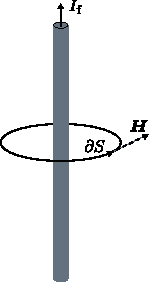
\includegraphics[height=0.7\textheight]{fig/lec02/Magnetic_field_strength_simple_conductor.pdf}
				\caption{Illustration of the magnetic field strength $\bm{H}$ around a simple conductor}
			\end{figure}
		\end{column}
		\end{columns}
\end{frame}

%%%%%%%%%%%%%%%%%%%%%%%%%%%%%%%%%%%%%%%%%%%%%%%%%%%%%%%%%%%%%
%% Ampere's circuital law %%
%%%%%%%%%%%%%%%%%%%%%%%%%%%%%%%%%%%%%%%%%%%%%%%%%%%%%%%%%%%%%
\begin{frame}
	\frametitle{Amp\`ere's circuital law: magnetic field strength example}
	\begin{columns}
		\begin{column}{0.55\textwidth}
			What is the free current $I_{\mathrm{f}}$ enclosed by the loop $\mathcal{C}$?
            \begin{itemize}
                \item The current $I_1$ flows in the direction of the loop $\mathcal{C}$ (according to right-hand rule).
                \item The current $I_1$ must be counted $N$ times due to the $N$ turns of wire around the loop $\mathcal{C}$.
                \item The current $I_2$ flows in the opposite direction of the loop $\mathcal{C}$ (according to right-hand rule).
                \item Result:
            \end{itemize}
            \vspace{0.25cm}
            \begin{equation*}
                I_\mathrm{f} = N \cdot I_1 - I_2.
            \end{equation*}
		\end{column}
        \hfill
		\begin{column}{0.45\textwidth}
			\begin{figure}
				\centering
				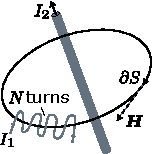
\includegraphics[height=0.5\textheight]{fig/lec02/Magnetic_field_strength_multiple_conductors.pdf}
				\caption{Arrangement with two electrical conductors}
			\end{figure}
		\end{column}
		\end{columns}
\end{frame}

%%%%%%%%%%%%%%%%%%%%%%%%%%%%%%%%%%%%%%%%%%%%%%%%%%%%%%%%%%%%%
%% Ampere's circuital law: magnetic flux %%
%%%%%%%%%%%%%%%%%%%%%%%%%%%%%%%%%%%%%%%%%%%%%%%%%%%%%%%%%%%%%
\begin{frame}
	\frametitle{Magnetic flux and flux linkage}
	\begin{columns}
		\begin{column}{0.575\textwidth}
			Variant for magnetic flux density $\bm{B}$:
            \begin{align}
                \mbox{Integral form:} \quad &\oint_{\mathcal{C}} \bm{B} \cdot \mathrm{d}\bm{l} = \mu_0 I,\\
                \mbox{Differential form:} \quad &\nabla \times \bm{B} = \mu_0\bm{J}. 
            \end{align}
            Here, $\mu_0$ is the permeability of free space, $\bm{J}$ is the total current density and $I$ is the total current enclosed by the loop $\mathcal{C}$. 
            \vspace{0.25cm}
            \begin{itemize}
                \item SI-unit: $[B] = \si{\tesla} = \si{\kilogram\per\ampere\second\squared}$
                \item Example contour $\mathcal{C}$  on the right covering $N$ turns and length $l$ (flux density within solenoid):
            \end{itemize}
            $$\oint_{\mathcal{C}} \bm{B} \cdot \mathrm{d}\bm{l} = N \mu_0 I  \Leftrightarrow B = \frac{N \mu_0 I}{l}$$
		\end{column}
        \hfill
		\begin{column}{0.425\textwidth}
            \vspace{-0.2cm}
			\begin{figure}
				\centering
				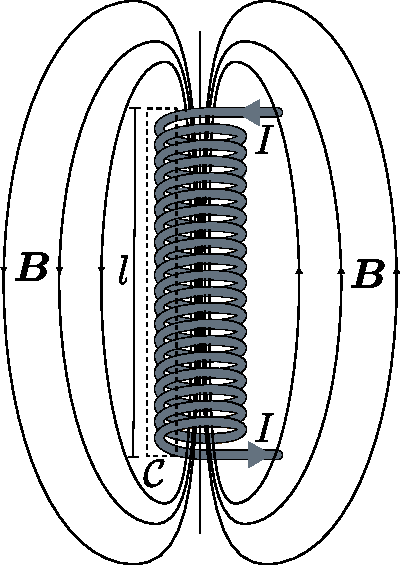
\includegraphics[height=0.68\textheight]{fig/lec02/Solenoid_Ampere_law.pdf}
				\caption{Magnetic flux $\Phi$ evaluated at the surface $\bm{S}$  (adapted from: \href{https://commons.wikimedia.org/wiki/File:Solenoid_and_Ampere_Law.png}{Wikimedia Commons}, Goodphy, \href{https://creativecommons.org/licenses/by-sa/4.0/deed.en}{CC BY-SA 4.0})}
			\end{figure}
		\end{column}
		\end{columns}
\end{frame}

%%%%%%%%%%%%%%%%%%%%%%%%%%%%%%%%%%%%%%%%%%%%%%%%%%%%%%%%%%%%%
%% Ampere's circuital law: magnetic flux %%
%%%%%%%%%%%%%%%%%%%%%%%%%%%%%%%%%%%%%%%%%%%%%%%%%%%%%%%%%%%%%
\begin{frame}
	\frametitle{Magnetic flux and flux linkage}
	\begin{columns}
		\begin{column}{0.575\textwidth}
			The magnetic flux $\Phi$ is the surface integral of the normal component of $\bm{B}$ over that surface:
            \begin{align}
                \Phi = \int_{S} \bm{B} \cdot \mathrm{d}\bm{S}. 
            \end{align}
            As there are no magnetic monopoles, the magnetic flux through a closed surface (which is covering a volume without holes) is always zero:
            \begin{align}
                \oint_{S} \bm{B} \cdot \mathrm{d}\bm{S} = 0.
            \end{align}
            The flux linkage $\Psi$ is the product of the magnetic flux $\Phi$ and the number of turns $N$ of a coil:
            \begin{align}
                \Psi = N  \Phi.
            \end{align}
		\end{column}
        \hfill
		\begin{column}{0.425\textwidth}
            \vspace{-0.2cm}
			\begin{figure}
				\centering
				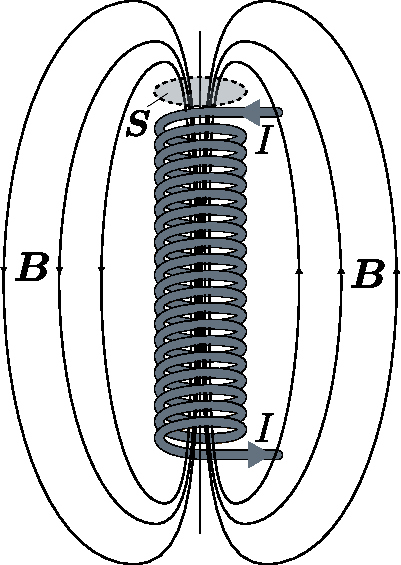
\includegraphics[height=0.68\textheight]{fig/lec02/Solenoid_Flux.pdf}
				\caption{Magnetic flux $\Phi$ evaluated at the surface $\bm{S}$  (adapted from: \href{https://commons.wikimedia.org/wiki/File:Solenoid_and_Ampere_Law.png}{Wikimedia Commons}, Goodphy, \href{https://creativecommons.org/licenses/by-sa/4.0/deed.en}{CC BY-SA 4.0})}
			\end{figure}
		\end{column}
		\end{columns}
\end{frame}

%%%%%%%%%%%%%%%%%%%%%%%%%%%%%%%%%%%%%%%%%%%%%%%%%%%%%%%%%%%%%
%% Boosting the magnet field with ferromagnetic materials %%
%%%%%%%%%%%%%%%%%%%%%%%%%%%%%%%%%%%%%%%%%%%%%%%%%%%%%%%%%%%%%
\begin{frame}
	\frametitle{Boosting the magnet field with ferromagnetic materials}
	\begin{columns}
		\begin{column}{0.575\textwidth}
			While $\bm{H}$ depends on the free currents applied to an object, $\bm{B}$ depends on the material properties of the object. In free space (vacuum), the relation is linear and represented by the magnetic constant $\mu_0$:
            \begin{align}
                \bm{B} = \mu_0 \bm{H} \quad \mbox{with} \quad \mu_0 \approx \SI{4 \pi e-7}{\newton\per\ampere\squared}.
            \end{align}
            To boost $\bm{B}$ for a given $\bm{H}$, ferromagnetic materials are typically used. These materials have a high relative magnetic permeability $\mu_{\mathrm{r}}$:
            \begin{align}
                \bm{B} = \mu \bm{H} = \mu_0 \mu_{\mathrm{r}} \bm{H}.
                \label{eq:linear_permeability} 
            \end{align}
            Note that $\mu_{\mathrm{r}}$ is a dimensionless quantity and that \eqref{eq:linear_permeability} assumes linear and isotropic material behavior.
		\end{column}
        \hfill
		\begin{column}{0.425\textwidth}
            \vspace{-0.2cm}
			\begin{figure}
				\centering
				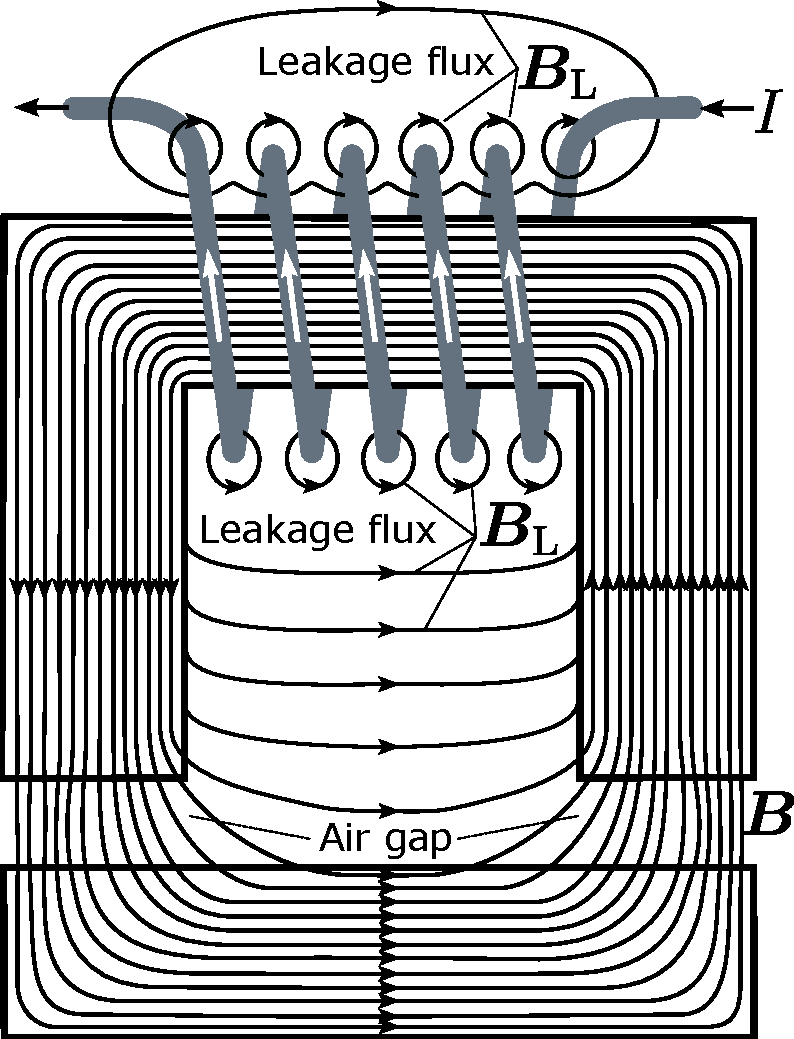
\includegraphics[height=0.68\textheight]{fig/lec02/Electromagnet_with_gap.pdf}
				\caption{Simplified magnetic field lines of an iron yoke with a coil  (adapted from: \href{https://en.m.wikipedia.org/wiki/File:Electromagnet_with_gap.svg}{Wikimedia Commons}, public domain)}
			\end{figure}
		\end{column}
		\end{columns}
\end{frame}

%%%%%%%%%%%%%%%%%%%%%%%%%%%%%%%%%%%%%%%%%%%%%%%%%%%%%%%%%%%%%
%% Relative permeability and magnetic saturation %%
%%%%%%%%%%%%%%%%%%%%%%%%%%%%%%%%%%%%%%%%%%%%%%%%%%%%%%%%%%%%%
\begin{frame}
	\frametitle{Relative permeability and magnetic saturation}
	\begin{columns}
		\begin{column}{0.575\textwidth}
			\begin{table}
            \centering
            \begin{tabular}{lc}
                \toprule
                Material & $\mu_{\mathrm{r}}$ (range)\\
                \midrule
                Air / copper / aluminum & $(\approx)$1 \\ 
                Iron (99.8\,\% pure) & 5000\\
                Electrical steel & 2000 - 35000\\
                Ferrite & 200 - 20000\\
                \bottomrule
            \end{tabular}
            \caption{Typical relative permeabilities of materials}
            \label{tab:rel_permeabilities}
            \end{table}
        Linear magnetic behavior ($\mu_{\mathrm{r}}=\mbox{const.}$) is only a local approximation. When considering larger $H$ ranges, the (differential) permeability becomes nonlinear:
        \begin{align}
            \mu_\mathrm{r}(H) =  \frac{\mathrm{d}B}{\mathrm{d}H}.
        \end{align}
		\end{column}
        \hfill
		\begin{column}{0.425\textwidth}
			\begin{figure}
				\centering
				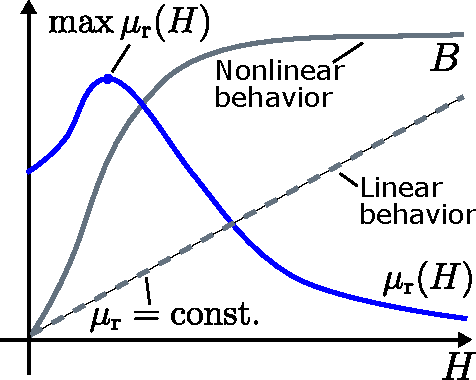
\includegraphics[height=0.5\textheight]{fig/lec02/Permeability_of_ferromagnet.pdf}
				\caption{Illustrative magnetisation curves for ferromagnets (and ferrimagnets) and corresponding permeabilities  (adapted from: \href{https://commons.wikimedia.org/wiki/File:Permeability_of_ferromagnet_by_Zureks.svg}{Wikimedia Commons}, public domain)}
			\end{figure}
		\end{column}
		\end{columns}
\end{frame}


%%%%%%%%%%%%%%%%%%%%%%%%%%%%%%%%%%%%%%%%%%%%%%%%%%%%%%%%%%%%%
%% Magnetic domains (1) %%
%%%%%%%%%%%%%%%%%%%%%%%%%%%%%%%%%%%%%%%%%%%%%%%%%%%%%%%%%%%%%
\begin{frame}
	\frametitle{Magnetic domains (1)}
    \begin{columns}
	\begin{column}{0.48\textwidth}
    \begin{itemize}
        \item Magnetic domains are regions within a material where the magnetic moments of atoms are aligned (``mini magnets'').
        \item The magnetization within each domain points in a uniform direction, but the magnetization of different domains may point in different directions.
    \end{itemize}
    \end{column}
    \hfill
    \begin{column}{0.52\textwidth}
        \begin{figure}
            \centering
            %\animategraphics[loop,autoplay, height=0.3\textheight]{8}{fig/lec02/Moving_magnetic_domains/Moving_magnetic_domains-}{0}{14}
            \movie{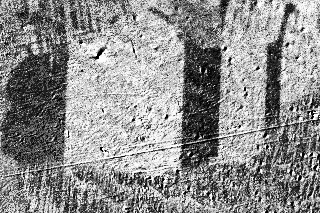
\includegraphics[height=0.3\textheight]{fig/lec02/Moving_magnetic_domains_preview.png}}{fig/lec02/Moving_magnetic_domains.gif}
            \caption{Animation of moving domain walls (source: \href{https://commons.wikimedia.org/wiki/File:Moving_magnetic_domains_by_Zureks.gif}{Wikimedia Commons}, Zureks, \href{https://creativecommons.org/licenses/by-sa/3.0/deed.en}{CC BY-SA 3.0})}
        \end{figure}
    \end{column}
\end{columns}
\begin{figure}
\begin{columns}
	\begin{column}{0.6\textwidth}
            \centering
            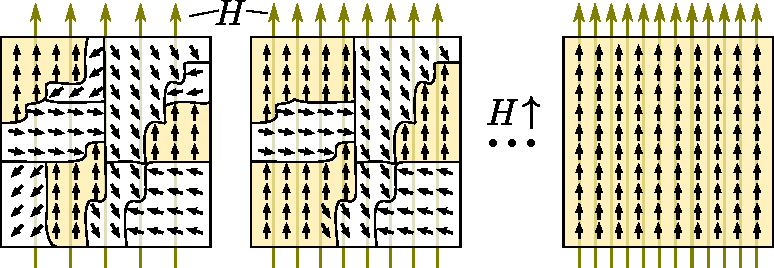
\includegraphics[width=0.9\textwidth]{fig/lec02/Growing-magnetic-domains.pdf}
    \end{column}
    \begin{column}{0.35\textwidth}
        \caption{\raggedright Change of magnetic domains due to an external magnetic field  (adapted from: \href{https://de.wikipedia.org/wiki/Datei:Growing-magnetic-domains.svg}{Wikimedia Commons}, M. Run, \href{https://creativecommons.org/licenses/by-sa/4.0/deed.en}{CC BY-SA 4.0})}
    \end{column}
\end{columns}
\end{figure}
\end{frame}

%%%%%%%%%%%%%%%%%%%%%%%%%%%%%%%%%%%%%%%%%%%%%%%%%%%%%%%%%%%%%
%% Magnetic domains (2) %%
%%%%%%%%%%%%%%%%%%%%%%%%%%%%%%%%%%%%%%%%%%%%%%%%%%%%%%%%%%%%%
\begin{frame}
	\frametitle{Magnetic domains (2)}
    \begin{itemize}
        \item A large region of material with a constant magnetization throughout creates a large magnetic field (diagram a) below). This requires a lot of magnetostatic energy stored in the field. 
        \item To reduce this energy, the sample can ``split'' into two domains, with the magnetization in opposite directions in each domain which reduces the overall field (diagram b) below).
        \item  To reduce the field energy further, each of these domains can split also, resulting in smaller parallel domains with magnetization in alternating directions, with smaller amounts of field outside the material (diagram c) below).
    \end{itemize}
\begin{figure}
\begin{columns}
	\begin{column}{0.55\textwidth}
            \centering
            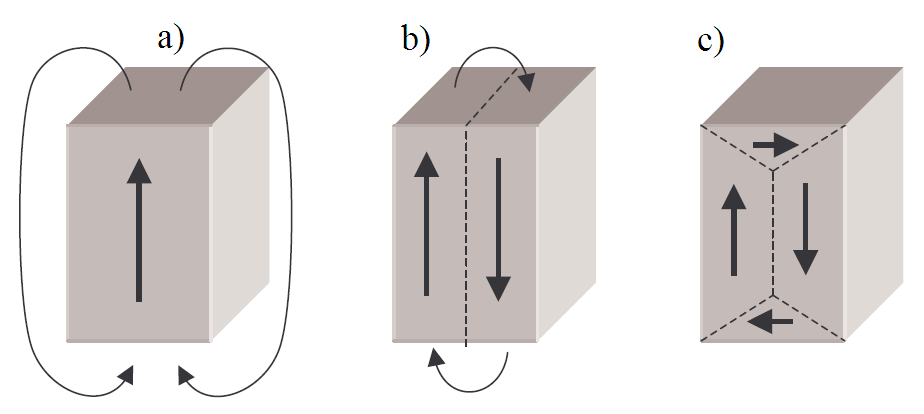
\includegraphics[width=0.8\textwidth]{fig/lec02/Magnetic_domains_energy_min.png}
    \end{column}
    \begin{column}{0.4\textwidth}
        \caption{\raggedright Simplified representation of the formation of magnetic domains on the basis of energy minimization  (source: \href{https://commons.wikimedia.org/wiki/File:Powstawanie_domen_by_Zureks.png}{Wikimedia Commons}, public domain)}
    \end{column}
\end{columns}
\end{figure}
\end{frame}

%%%%%%%%%%%%%%%%%%%%%%%%%%%%%%%%%%%%%%%%%%%%%%%%%%%%%%%%%%%%%
%% Hysteresis %%
%%%%%%%%%%%%%%%%%%%%%%%%%%%%%%%%%%%%%%%%%%%%%%%%%%%%%%%%%%%%%
\begin{frame}
	\frametitle{Hysteresis}
	\begin{columns}
		\begin{column}{0.575\textwidth}
            \begin{itemize}
                \item Material defects lead to small, random jumps in magnetization called Barkhausen jumps.
                \item Domain walls move there irregular and depend on the history of the magnetization process (dynamic system).
            \end{itemize}
			\begin{figure}
                \centering
                \movie{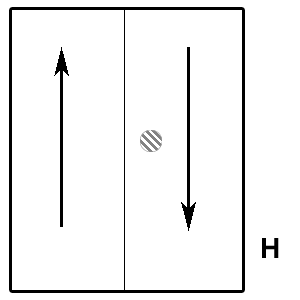
\includegraphics[height=0.3\textheight]{fig/lec02/Barkhausen_jump_preview.png}}{fig/lec02/Barkhausen_jump.gif}
                \caption{Animation of the Barkhausen jump (source: \href{https://commons.wikimedia.org/wiki/File:Barkhausensprung.gif}{Wikimedia Commons},  public domain)}
            \end{figure}
		\end{column}
        \hfill
		\begin{column}{0.425\textwidth}
            \vspace{-0.2cm}
			\begin{figure}
				\centering
				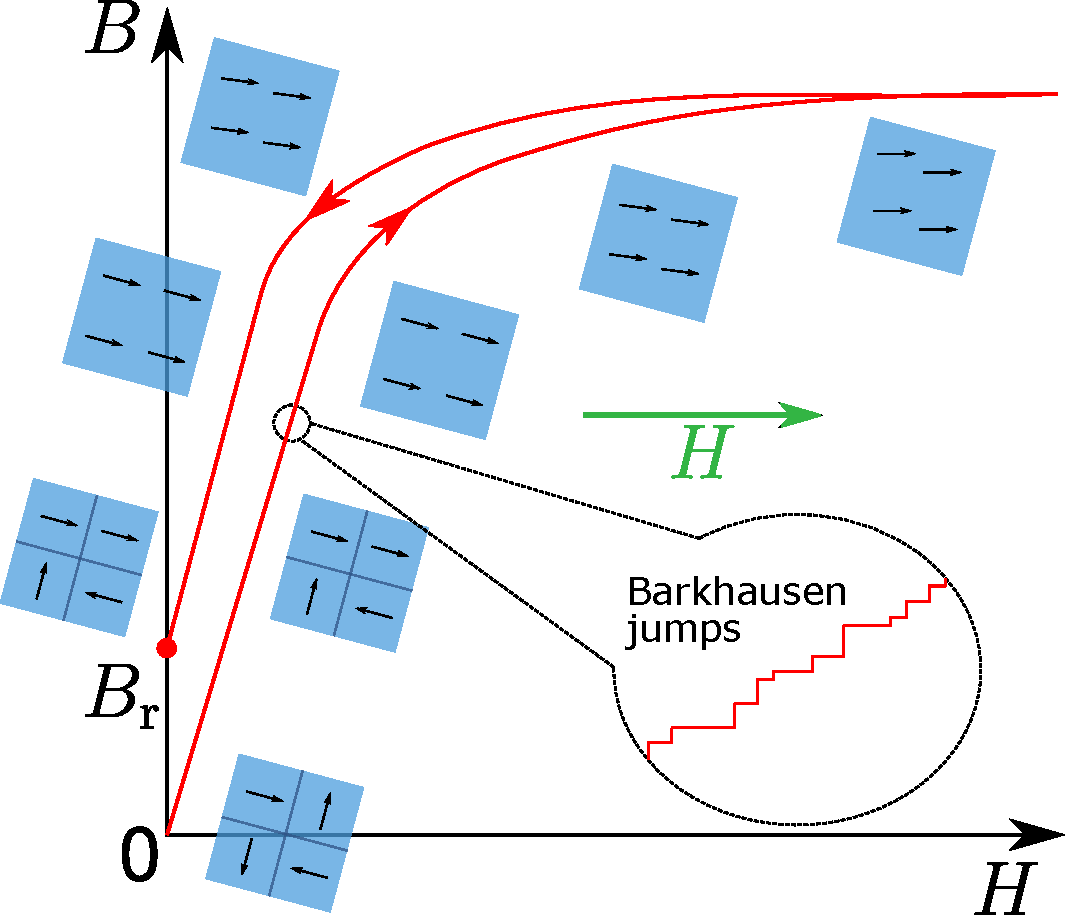
\includegraphics[height=0.5\textheight]{fig/lec02/Ferromagnet_magnetization_and_magnetic_domains_and_hysteresis.pdf}
				\caption{Simplified hysteresis curve in first quadrant with magnetic domains illustration (adapted from: \href{https://commons.wikimedia.org/wiki/File:Ferromagnet_magnetization_and_magnetic_domains_and_hysteresis.svg}{Wikimedia Commons}, Fralama, \href{https://creativecommons.org/licenses/by-sa/3.0/deed.enn}{CC BY-SA 3.0})}
			\end{figure}
		\end{column}
		\end{columns}
\end{frame}

 % Fundamental electromagnetic principles
\part{DC machines}
\title{DC machines}  
\date{}  
\frame{\titlepage} 

%%%%%%%%%%%%%%%%%%%%%%%%%%%%%%%%%%%%%%%%%%%%%%%%%%%%%%%%%%%%%
%% Homopolar / unipolar machines %%
%%%%%%%%%%%%%%%%%%%%%%%%%%%%%%%%%%%%%%%%%%%%%%%%%%%%%%%%%%%%%
\begin{frame}
	\frametitle{Homopolar / unipolar machines}
    \vspace{-0.3cm}
	\begin{figure}
		\centering
		\begin{subfigure}[b]{0.49\textwidth}
			\centering
			\movie{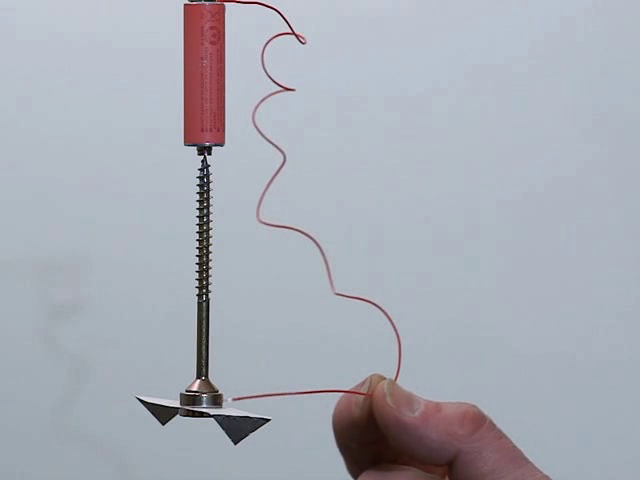
\includegraphics[height=0.4\textheight]{fig/lec03/homopolar_machine_video.png}}{fig/lec03/homopolar_machine_video.mp4}
            \vspace{0.75cm}
			\caption{Video of an operating homopolar machine (source: \href{https://de.wikipedia.org/wiki/Datei:Homopolarmotor_MAQ03891_smial_wp.ogv}{Wikimedia Commons}, Smial, \href{https://artlibre.org/licence/lal/en/}{Free Art License})}
		\end{subfigure}
		\hfill
		\begin{subfigure}[b]{0.49\textwidth}
			\centering
			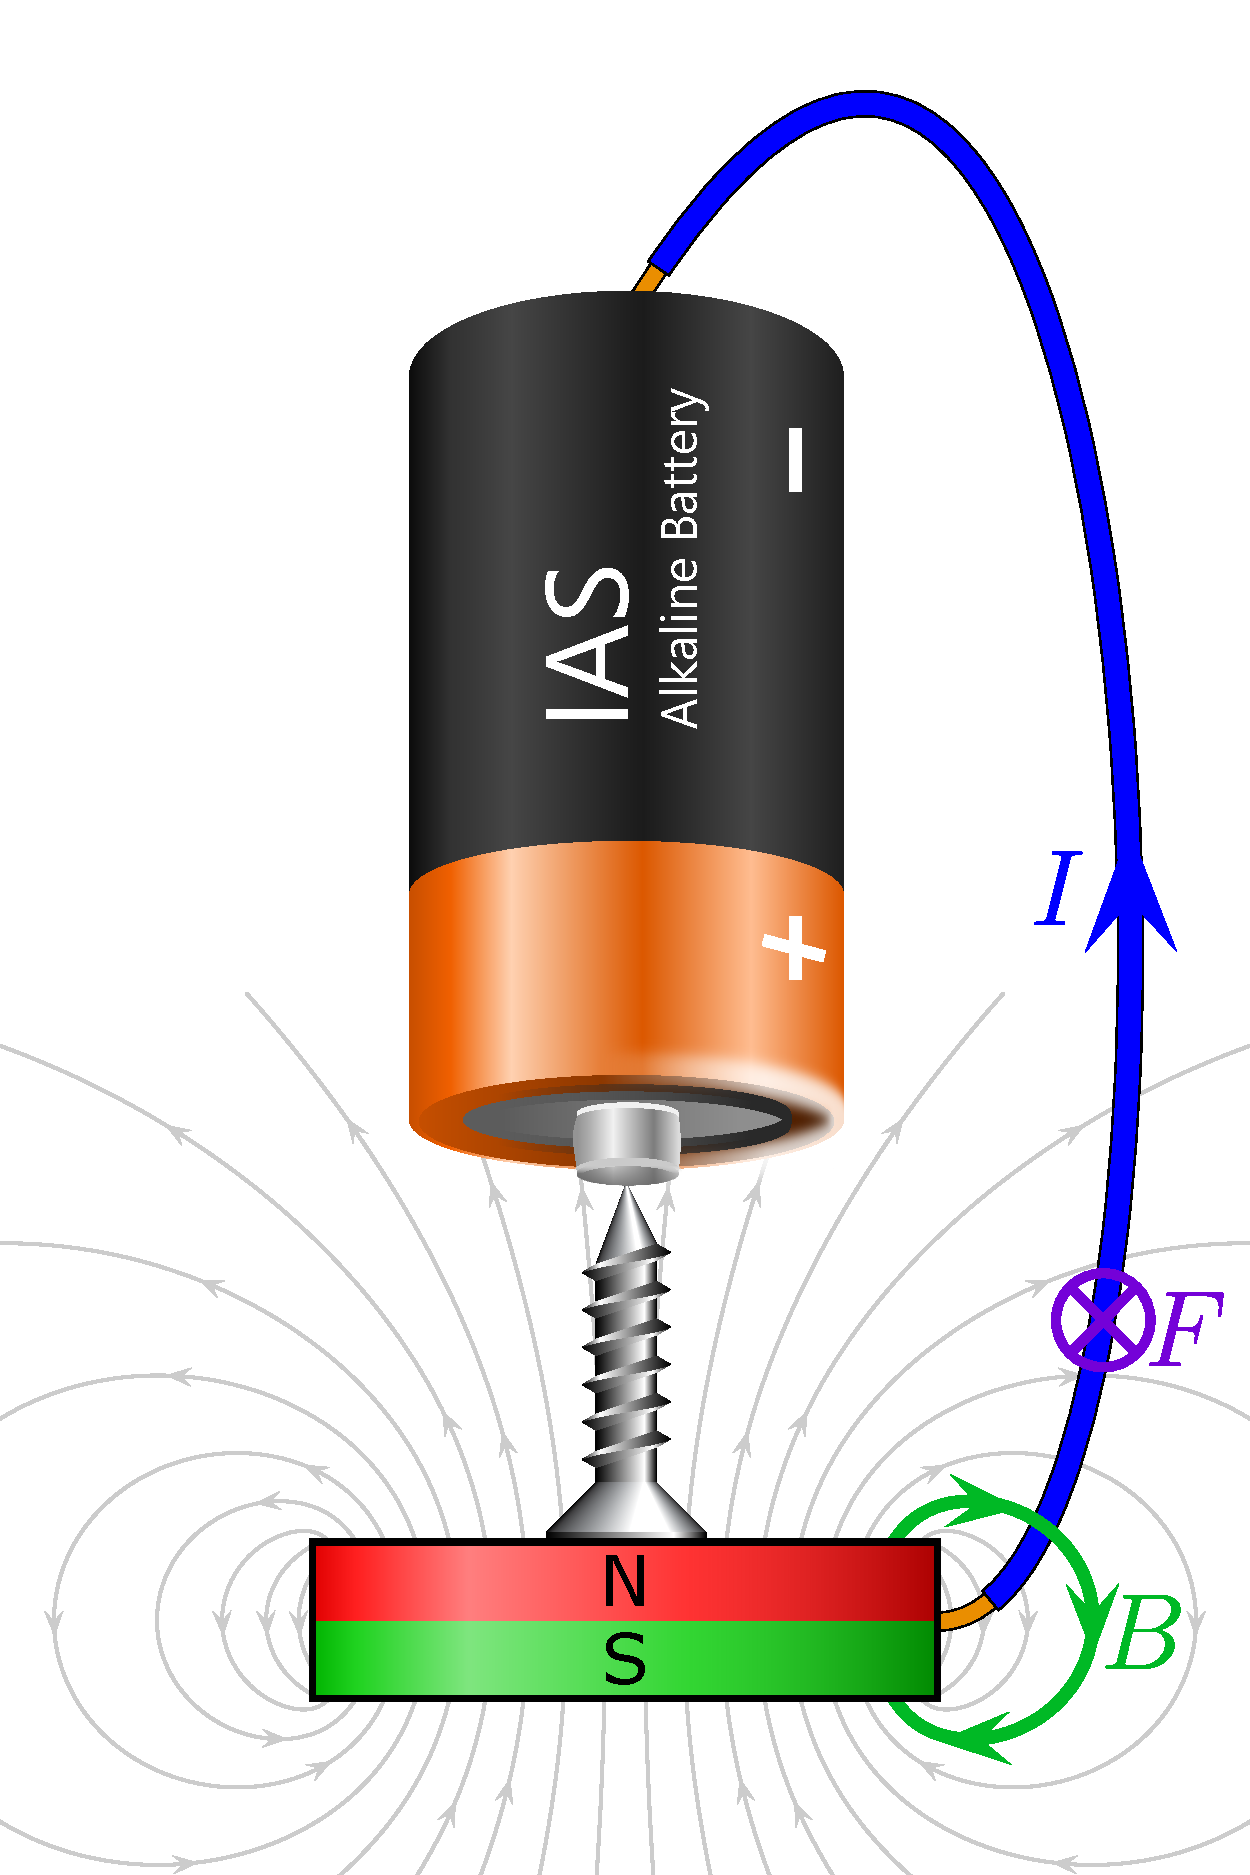
\includegraphics[width=0.47\textwidth]{fig/lec03/Homopolar_machine.pdf}
			\caption{Electric current, magnetic field and Lorentz force (adapted: \href{https://commons.wikimedia.org/wiki/File:Homopolar-motor.svg}{Wikimedia Commons}, M. Run, \href{https://creativecommons.org/licenses/by-sa/4.0/deed.en}{CC BY-SA})}
		\end{subfigure}
		\caption{Working principle of homopolar machines demonstrated with a simple permanent magnet, battery and screw design} 
        \label{fig:Homopolar_machine}
	\end{figure}
\end{frame}


%%%%%%%%%%%%%%%%%%%%%%%%%%%%%%%%%%%%%%%%%%%%%%%%%%%%%%%%%%%%%
%% Homopolar / unipolar machines (cont.) %%
%%%%%%%%%%%%%%%%%%%%%%%%%%%%%%%%%%%%%%%%%%%%%%%%%%%%%%%%%%%%%
\begin{frame}
	\frametitle{Homopolar / unipolar machines (cont.)}
    \begin{columns}
		\begin{column}{0.5\textwidth}
            \begin{itemize}
                \item  Homopolar machines are the simplest form of electric machines.
                \item They are also true DC machines, as the current and flux paths are unidirectional.
                \item<2-> The general design prevents connecting multiple rotor turns in series to increase the voltage, that is, only a relatively low voltage is induced.
                \item<3-> Consequently, homopolar machines require high currents (in the order of  \si{\kilo\ampere} or even \si{\mega\ampere}) to reach a useful power range which limited their application.
            \end{itemize}
		\end{column}
        \hfill
		\begin{column}{0.49\textwidth}
			\begin{figure}
				\centering
				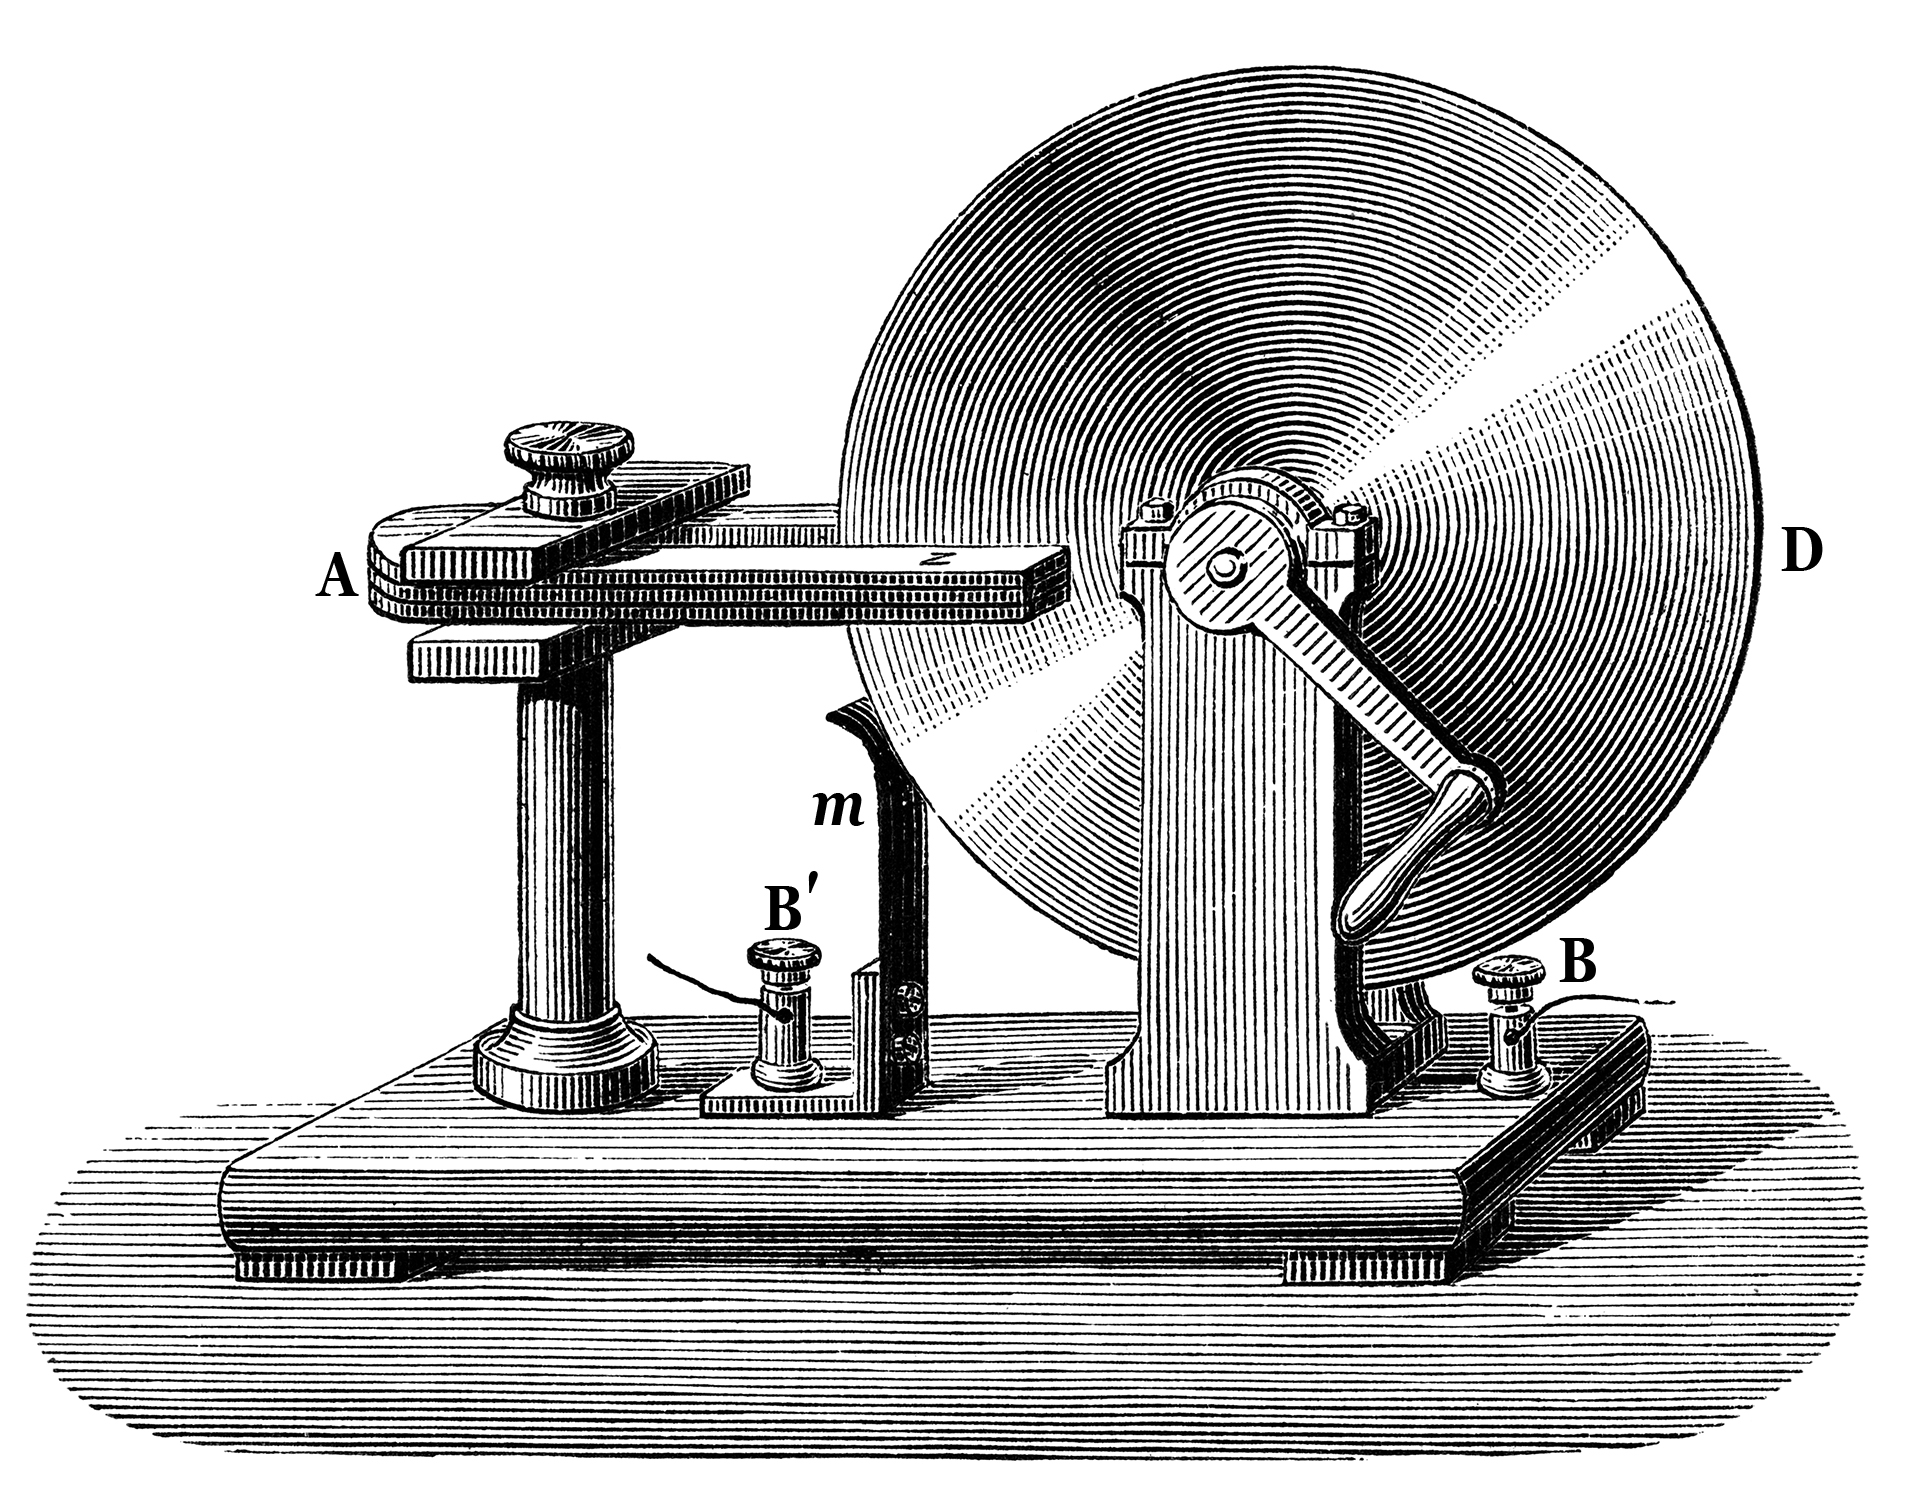
\includegraphics[width=0.8\textwidth]{fig/lec03/Faraday_disk_generator.jpg}
				\caption{The Faraday disk: another homopolar machine (source: \href{https://commons.wikimedia.org/wiki/File:Faraday_disk_generator.jpg}{Wikimedia Commons}, public domain)}
			\end{figure}
		\end{column}
		\end{columns}
\end{frame}

%%%%%%%%%%%%%%%%%%%%%%%%%%%%%%%%%%%%%%%%%%%%%%%%%%%%%%%%%%%%%
%% Working principle of usual DC machines %%
%%%%%%%%%%%%%%%%%%%%%%%%%%%%%%%%%%%%%%%%%%%%%%%%%%%%%%%%%%%%%
\begin{frame}
	\frametitle{Working principle of usual DC machines}
    \begin{columns}
		\begin{column}{0.5\textwidth}
            Let's consider \figref{fig:Simple_yoke_coil} and assume that the flux density $B$ is constant in the air gap and that the conductor loop has the axial length $l_\mathrm{z}$. \onslide<2->{According to the Lorentz force we have
			\begin{equation}
				F = I_\mathrm{a} B l_\mathrm{z} .
			\end{equation}}%  
			\onslide<3->{The torque $T$ on the conductor loop is given by
			\begin{equation}
				T = 2 F \frac{d}{2} \cos\left(\varepsilon\right) = I_\mathrm{a} B l_\mathrm{z} d \cos\left(\varepsilon\right).
			\end{equation}}%
			\onslide<4->{If the loop spins with an angular velocity $\omega$, mechanical power $P_\mathrm{me} = T\omega$ is transferred. 
			\\[1em]}%
			\onslide<5->{\textbf{Question:} What is happening if the coil is outside the magnetic field?}
		\end{column}
        \hfill
		\begin{column}{0.49\textwidth}
			\begin{figure}
				\centering
				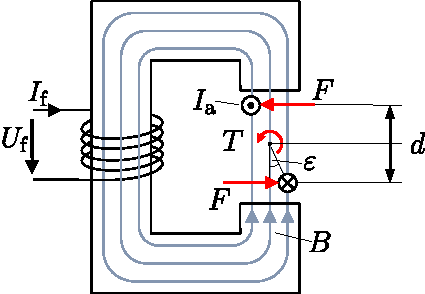
\includegraphics[width=0.9\textwidth]{fig/lec03/Simple_yoke_coil.pdf}
				\caption{Torque on a conductor loop (adapted from J.~B\"ocker, \textit{Elektrische Antriebstechnik}, Paderborn University, 2020)}
				\label{fig:Simple_yoke_coil}
			\end{figure}
		\end{column}
		\end{columns}
\end{frame}

%%%%%%%%%%%%%%%%%%%%%%%%%%%%%%%%%%%%%%%%%%%%%%%%%%%%%%%%%%%%%
%% DC-machine cross section %%
%%%%%%%%%%%%%%%%%%%%%%%%%%%%%%%%%%%%%%%%%%%%%%%%%%%%%%%%%%%%%
\begin{frame}
	\frametitle{DC-machine cross section}
    \begin{columns}
		\begin{column}{0.42\textwidth}
            \begin{itemize}
				\item To ensure a quasi-continous torque, the current through the conductor loop(s) in the rotor must have a constant direction.
				\item<2-> This is achieved by using a commutator (brushes).
				\item<3-> Compared to homopolar machines, DC machines require a mechanical rectification of the current.
			\end{itemize}
		\end{column}
        \hfill
		\begin{column}{0.55\textwidth}
			\begin{figure}
				\centering
				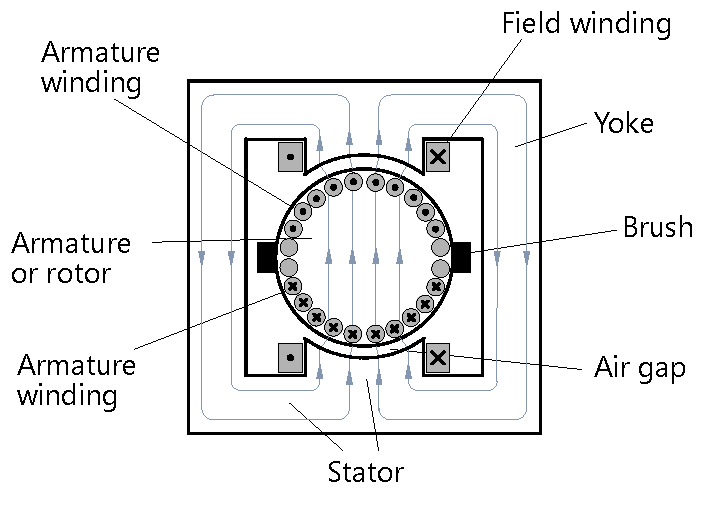
\includegraphics[width=0.925\textwidth]{fig/lec03/DC_machine_cross_section.pdf}
				\caption{Simplified DC machine cross section (adapted from J.~B\"ocker, \textit{Elektrische Antriebstechnik}, Paderborn University, 2020)}
				\label{fig:DC_machine_cross_section}
			\end{figure}
		\end{column}
		\end{columns}
\end{frame}

%%%%%%%%%%%%%%%%%%%%%%%%%%%%%%%%%%%%%%%%%%%%%%%%%%%%%%%%%%%%%
%% Commutation %%
%%%%%%%%%%%%%%%%%%%%%%%%%%%%%%%%%%%%%%%%%%%%%%%%%%%%%%%%%%%%%
\begin{frame}
	\frametitle{Commutation}
    \begin{figure}
		\centering
		\movie{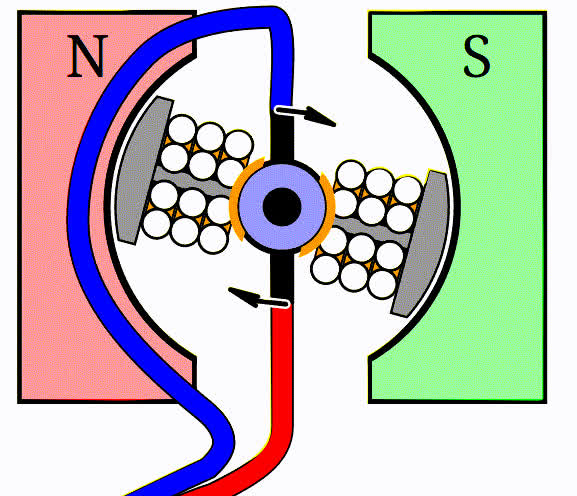
\includegraphics[height=0.65\textheight]{fig/lec03/DC_machine_simple_animation.jpeg}}{fig/lec03/DC_machine_simple_animation.gif}
		\caption{Animation of the commutation process \\(source: \href{https://commons.wikimedia.org/wiki/File:Animation_einer_Gleichstrommaschine_(Variante-Langsam).gif}{Wikimedia Commons}, M. Frey, \href{https://creativecommons.org/licenses/by-sa/3.0/deed.en}{CC BY-SA 3.0})}
	\end{figure}
\end{frame}

%%%%%%%%%%%%%%%%%%%%%%%%%%%%%%%%%%%%%%%%%%%%%%%%%%%%%%%%%%%%%
%% Armature and commutator %%
%%%%%%%%%%%%%%%%%%%%%%%%%%%%%%%%%%%%%%%%%%%%%%%%%%%%%%%%%%%%%
\begin{frame}
	\frametitle{Armature and commutator}
    \begin{figure}
		\centering
		\begin{subfigure}[b]{0.49\textwidth}
			\centering
			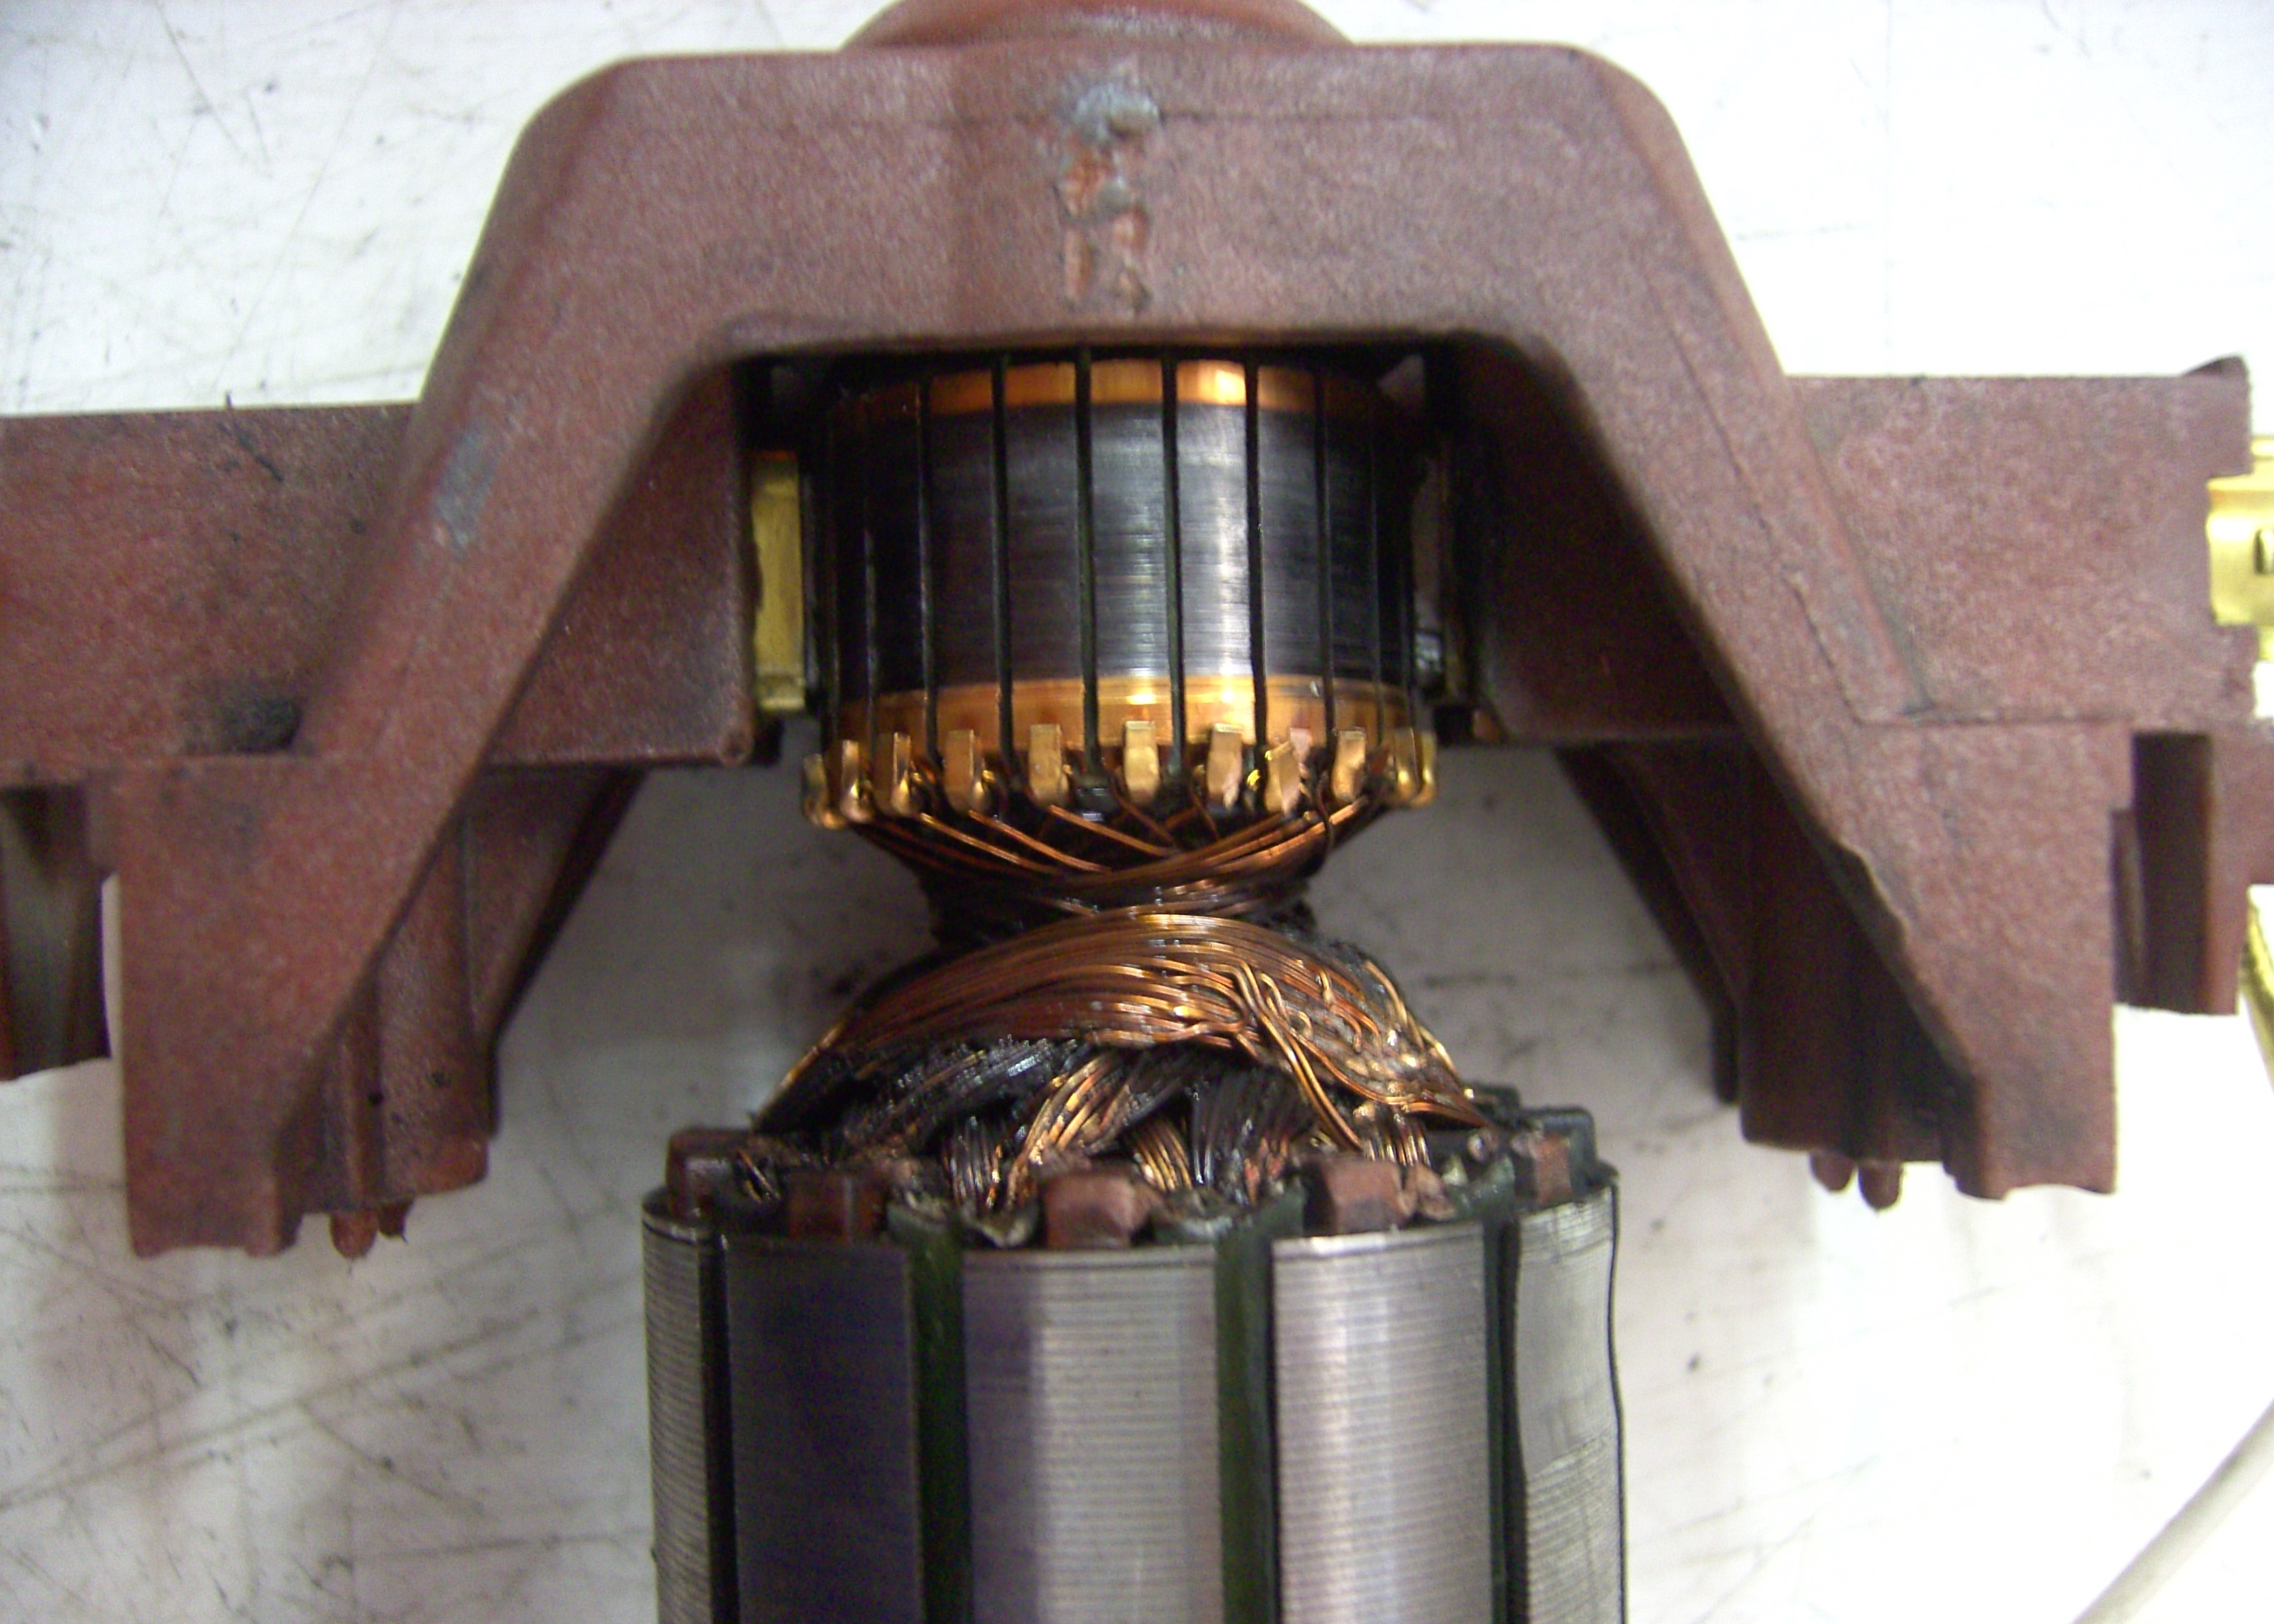
\includegraphics[width=0.85\textwidth]{fig/lec03/Commutator_Universalmachine.jpg}
			\caption{Commutator with brushes and springs (source: \href{https://commons.wikimedia.org/wiki/File:Kommutator_eines_Universalmotor.JPGg}{Wikimedia Commons}, Marrrci, \href{https://creativecommons.org/licenses/by-sa/3.0/deed.en}{CC BY-SA 3.0})}
		\end{subfigure}
		\hfill
		\begin{subfigure}[b]{0.49\textwidth}
			\centering
			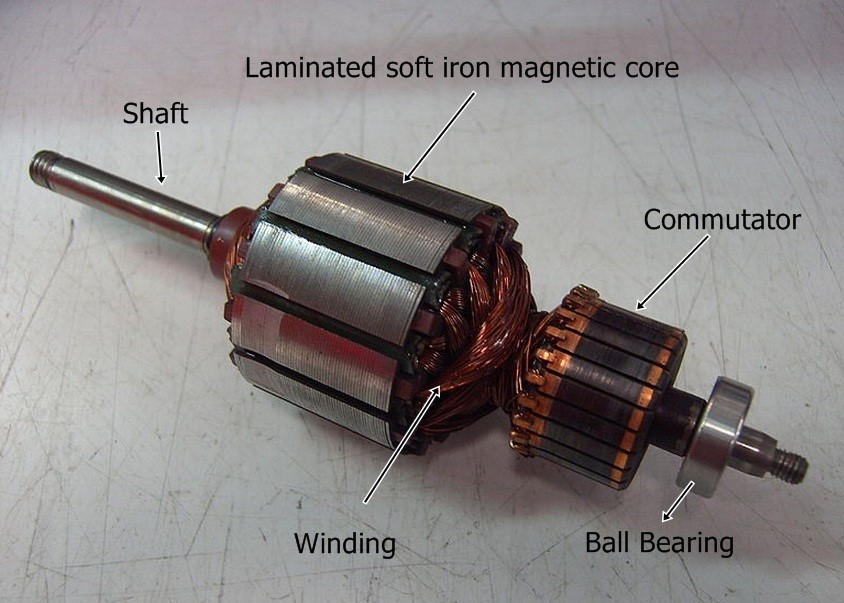
\includegraphics[width=0.85\textwidth]{fig/lec03/DC_armature_example.jpg}
			\caption{DC machine armature with commutator (source: \href{https://commons.wikimedia.org/wiki/File:Motor_rotor.jpg}{Wikimedia Commons}, public domain)}
		\end{subfigure}
		\caption{Examples of commutators and armatures} 
        \label{fig:Armature_and_commutator}
	\end{figure}
\end{frame}

%%%%%%%%%%%%%%%%%%%%%%%%%%%%%%%%%%%%%%%%%%%%%%%%%%%%%%%%%%%%%
%% Armature and commutator (cont.) %%
%%%%%%%%%%%%%%%%%%%%%%%%%%%%%%%%%%%%%%%%%%%%%%%%%%%%%%%%%%%%%
\begin{frame}
	\frametitle{Armature and commutator (cont.)}
    \begin{figure}
		\centering
		\begin{subfigure}[b]{0.49\textwidth}
			\centering
			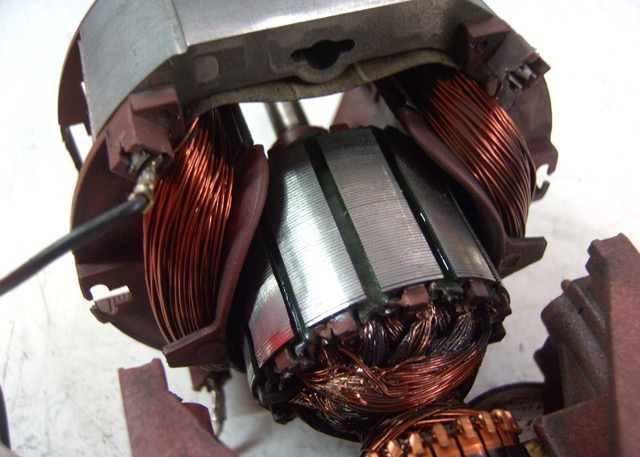
\includegraphics[width=0.85\textwidth]{fig/lec03/Stator_Rotor_Universalmachine.jpg}
			\caption{Armature inside stator (source: \href{https://commons.wikimedia.org/wiki/File:Universalmotor_1.JPG}{Wikimedia Commons}, Marrrci, \href{https://creativecommons.org/licenses/by-sa/3.0/deed.en}{CC BY-SA 3.0})}
		\end{subfigure}
		\hfill
		\begin{subfigure}[b]{0.49\textwidth}
			\centering
			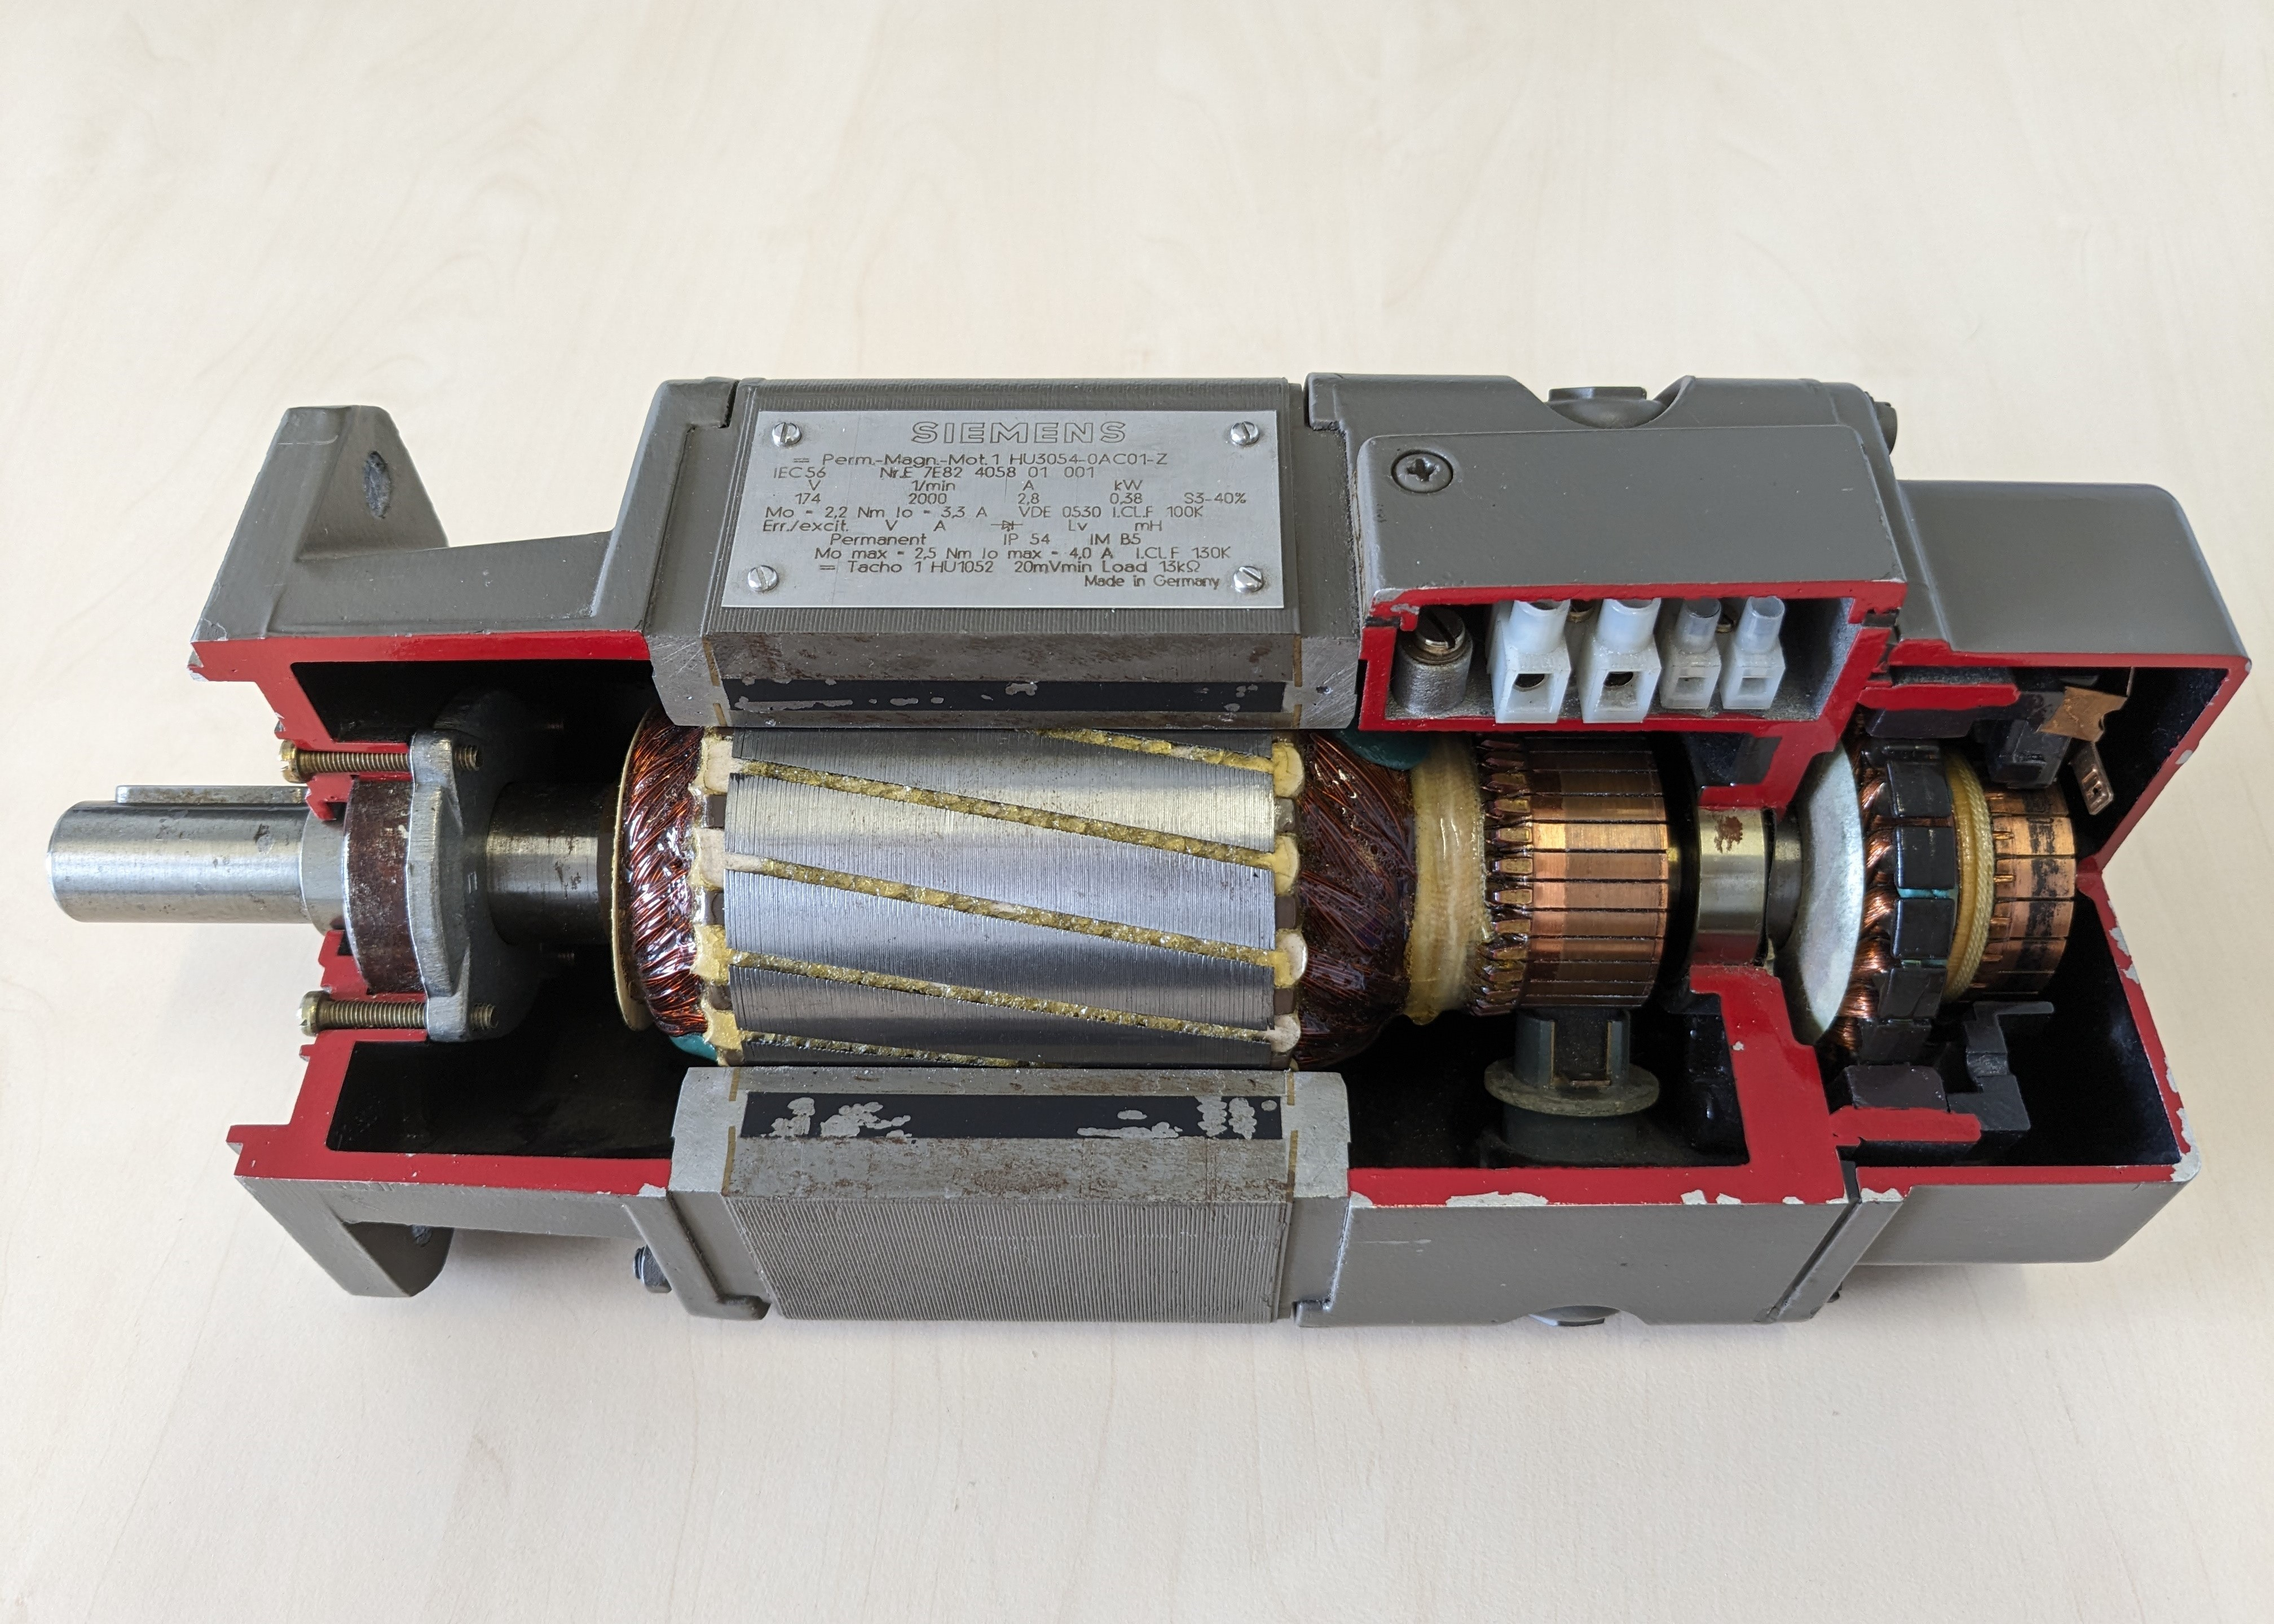
\includegraphics[width=0.85\textwidth]{fig/lec03/DC_Machine_PM.jpg}
			\caption{DC machine with permanent magnet excitation and tacho speed sensor}
		\end{subfigure}
		\caption{Examples of commutators and armatures (cont.)} 
        \label{fig:Armature_and_commutator_02}
	\end{figure}
\end{frame}

%%%%%%%%%%%%%%%%%%%%%%%%%%%%%%%%%%%%%%%%%%%%%%%%%%%%%%%%%%%%%
%% Basic structure of the armature %%
%%%%%%%%%%%%%%%%%%%%%%%%%%%%%%%%%%%%%%%%%%%%%%%%%%%%%%%%%%%%%
\begin{frame}
	\frametitle{Basic structure of the armature}
    \begin{figure}
        \centering
        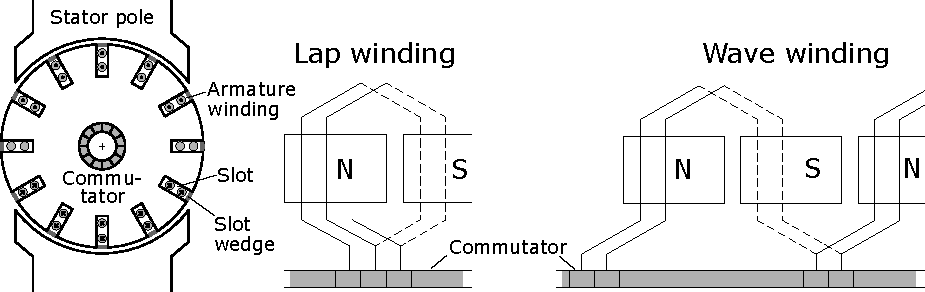
\includegraphics[width=0.925\textwidth]{fig/lec03/Armature_slots.pdf}
        \caption{Cross section of a drum-type armature including principle winding schemes (adapted from W.~Novender, \textit{Elektrische Maschinen}, Technische Hochschule Mittelhessen, 2023)}
    \end{figure}
\end{frame}

%%%%%%%%%%%%%%%%%%%%%%%%%%%%%%%%%%%%%%%%%%%%%%%%%%%%%%%%%%%%%
%% Commutation process with an armature lap winding %%
%%%%%%%%%%%%%%%%%%%%%%%%%%%%%%%%%%%%%%%%%%%%%%%%%%%%%%%%%%%%%
\begin{frame}
	\frametitle{Commutation process with an armature lap winding}
	\vspace{-0.1cm}
    \begin{figure}
        \centering
        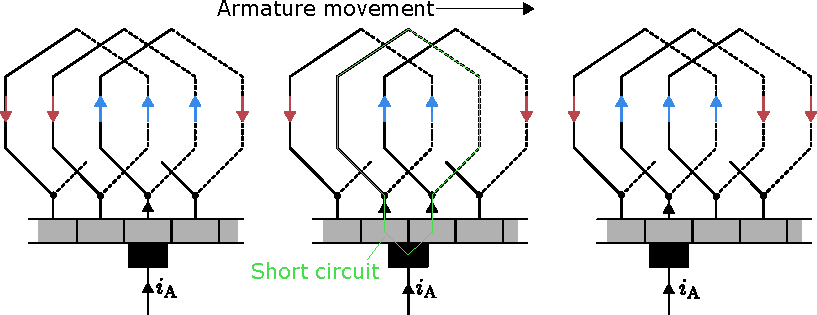
\includegraphics[height=0.6\textheight]{fig/lec03/Commutation_process_lap_winding.pdf}
        \caption{Three still images of the commutation process with a simplified winding representation (from left to right): when the brush touches two commutator segments, the according conductor loop is short-circuited and the current is reduced to zero. The brush then moves to the next commutator segment and the current starts flowing again but in the opposite direction (adapted from W.~Novender, \textit{Elektrische Maschinen}, Technische Hochschule Mittelhessen, 2023).}
    \end{figure}
\end{frame}

%%%%%%%%%%%%%%%%%%%%%%%%%%%%%%%%%%%%%%%%%%%%%%%%%%%%%%%%%%%%%
%% DC machines with multiple pole pairs %%
%%%%%%%%%%%%%%%%%%%%%%%%%%%%%%%%%%%%%%%%%%%%%%%%%%%%%%%%%%%%%
\begin{frame}
	\frametitle{DC machines with multiple pole pairs}
    \begin{columns}
		\begin{column}{0.42\textwidth}
            \begin{itemize}
				\item To reduce the effective length per armature conductor loop, the winding can form multiple pole pairs $p$.
				\item<2-> This will reduce the inductance per loop which is beneficial for the commutation process.
				\item<3-> The stator excitation must meet the same number of pole pairs.
				\item<4-> Given some inner stator diameter $d_\mathrm{s}$, the resulting pole pitch is:
			\end{itemize}
			\onslide<4->{\begin{equation}
				\tau_\mathrm{p} = \frac{\pi d_\mathrm{s}}{2p}, \quad \rho_\mathrm{p} = \frac{\pi}{p} .
			\end{equation}}%
		\end{column}
        \hfill
		\begin{column}{0.55\textwidth}
			\begin{figure}
				\centering
				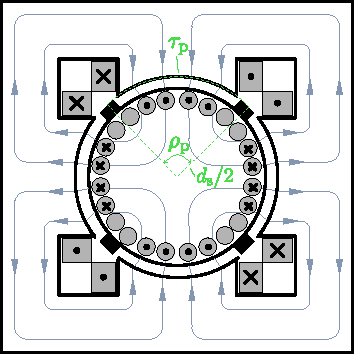
\includegraphics[width=0.64\textwidth]{fig/lec03/DC_machine_cross_section_two_pole_pairs.pdf}
				\caption{Simplified DC machine cross section with $p=2$ pole pairs (adapted from J.~B\"ocker, \textit{Elektrische Antriebstechnik}, Paderborn University, 2020)}
				\label{fig:DC_machine_cross_section_two_pole_pairs}
			\end{figure}
		\end{column}
		\end{columns}
\end{frame}

%%%%%%%%%%%%%%%%%%%%%%%%%%%%%%%%%%%%%%%%%%%%%%%%%%%%%%%%%%%%%
%% Winding characteristics (cont.) %%
%%%%%%%%%%%%%%%%%%%%%%%%%%%%%%%%%%%%%%%%%%%%%%%%%%%%%%%%%%%%%
\begin{frame}
	\frametitle{Armature winding characteristics}
	For describing the armature winding layout, the following parameters are introduced:
	\begin{gather*}
		Q: \mbox{number of slots}, \quad N_\mathrm{c}: \mbox{number of conductor turns per coil}, \\ K: \mbox{number of commutator elements}, \quad u = K/Q: \mbox{slot to commutator ratio}, \\z_\mathrm{a} = 2 K N_\mathrm{c}: \mbox{total number of armature conductors}.
	\end{gather*}
    \begin{figure}
        \centering
        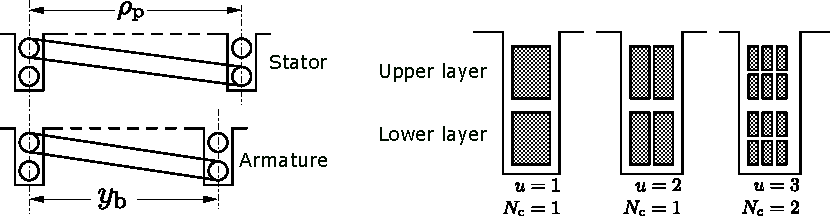
\includegraphics[height=0.35\textheight]{fig/lec03/Lap_winding_characteristics.pdf}
        \caption{Coil width and slot design characteristics (adapted from W.~Novender, \textit{Elektrische Maschinen}, Technische Hochschule Mittelhessen, 2023)}
		\label{fig:Lap_winding_characteristics}
    \end{figure}
\end{frame}

%%%%%%%%%%%%%%%%%%%%%%%%%%%%%%%%%%%%%%%%%%%%%%%%%%%%%%%%%%%%%
%% Double layer winding %%
%%%%%%%%%%%%%%%%%%%%%%%%%%%%%%%%%%%%%%%%%%%%%%%%%%%%%%%%%%%%%
\begin{frame}
	\frametitle{Double layer winding}
	\begin{itemize}
		\item The forward conductor of one coil and the return conductor of another coil are placed in the same slot. This is the common winding scheme (although not limited to it).
		\item Enables chording of the winding ($\rho_\mathrm{p}\neq y_\mathrm{b}$), another degree of freedom for the machine design (cf. \figref{fig:Lap_winding_characteristics}).
	\end{itemize}
    \begin{figure}
        \centering
        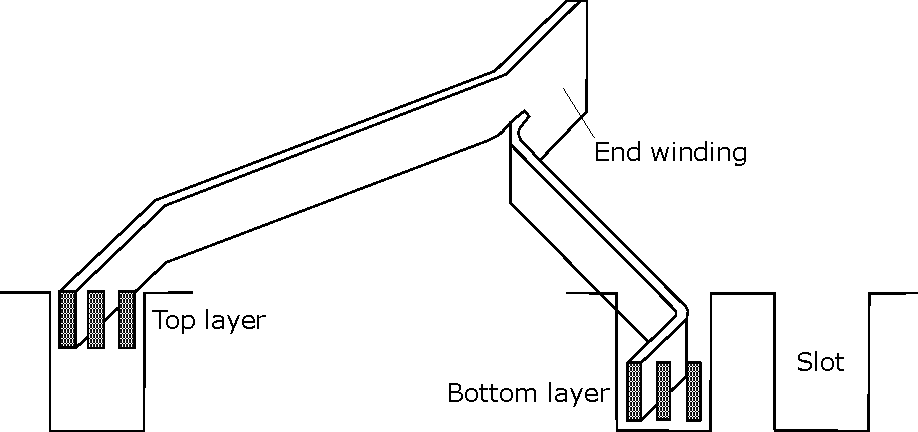
\includegraphics[height=0.45\textheight]{fig/lec03/Double_layer_winding.pdf}
        \caption{Double layer winding with $u=3$ with a solid conductor element (which can be pre-manufactured for cost reasons -- inspired from A. Binder, \textit{Elektrische Maschinen und Antriebe}, Vol. 2, Springer, 2017)}
    \end{figure}
\end{frame}

%%%%%%%%%%%%%%%%%%%%%%%%%%%%%%%%%%%%%%%%%%%%%%%%%%%%%%%%%%%%%
%% Lap winding characteristics %%
%%%%%%%%%%%%%%%%%%%%%%%%%%%%%%%%%%%%%%%%%%%%%%%%%%%%%%%%%%%%%
\begin{frame}
	\frametitle{Lap winding characteristics}
    \begin{columns}
		\begin{column}{0.42\textwidth}
            \begin{itemize}
				\item Back pitch $y_\mathrm{b}$: coil span from the back end
				\item<2-> Front pitch $y_\mathrm{f}$: coil span from the front end
				\item<3-> Resultant pitch $y_\mathrm{r}$: distance between two consecutive coils
				\item<4-> Commutator pitch $y_\mathrm{c}$: distance between two consecutive commutator segments
			\end{itemize}
			\vspace{-0.4cm}
			\onslide<5->{\begin{varblock}{Progressive winding}
				\figref{fig:Lap_winding_distances} shows a progressive winding layout with $y_\mathrm{b} > y_\mathrm{f}$, i.e., the coils do not cross themselves.
			\end{varblock}}%
		\end{column}
        \hfill
		\begin{column}{0.55\textwidth}
			\begin{figure}
				\centering
				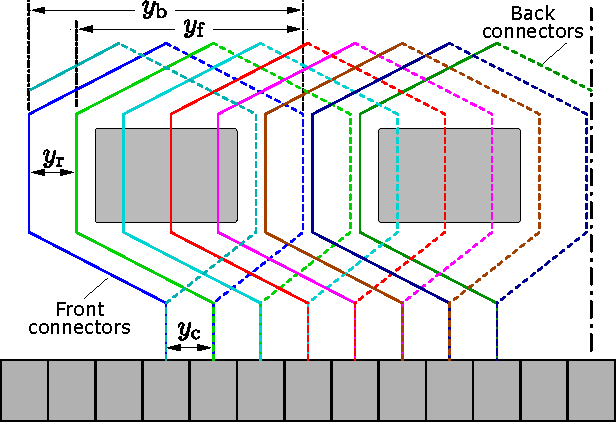
\includegraphics[width=0.85\textwidth]{fig/lec03/Lap_winding_distances.pdf}
				\caption{Distance definitions of the armature lap winding (adapted from W.~Novender, \textit{Elektrische Maschinen}, Technische Hochschule Mittelhessen, 2023)}
				\label{fig:Lap_winding_distances}
			\end{figure}
		\end{column}
		\end{columns}
\end{frame}

%%%%%%%%%%%%%%%%%%%%%%%%%%%%%%%%%%%%%%%%%%%%%%%%%%%%%%%%%%%%%
%% Lap winding characteristics (cont.) %%
%%%%%%%%%%%%%%%%%%%%%%%%%%%%%%%%%%%%%%%%%%%%%%%%%%%%%%%%%%%%%
\begin{frame}
	\frametitle{Lap winding characteristics (cont.)}
    \begin{columns}
		\begin{column}{0.42\textwidth}
			\begin{varblock}{Retrogressive winding}
				\figref{fig:Lap_winding_distances_retrogressive} shows a Retrogressive winding layout with $y_\mathrm{b} < y_\mathrm{f}$, i.e., each coil crosses itself.
			\end{varblock}
			\begin{itemize}
				\item<2-> Retrogressive windings require more conductor material due to the crossing of the coils and, therefore, are less common.
				\item<3-> Technical feasibility requires $y_\mathrm{b} - y_\mathrm{f} = \pm y_\mathrm{c}$, i.e., the lap winding progresses or retrogresses by one commutator element.
			\end{itemize}
		\end{column}
        \hfill
		\begin{column}{0.55\textwidth}
			\begin{figure}
				\centering
				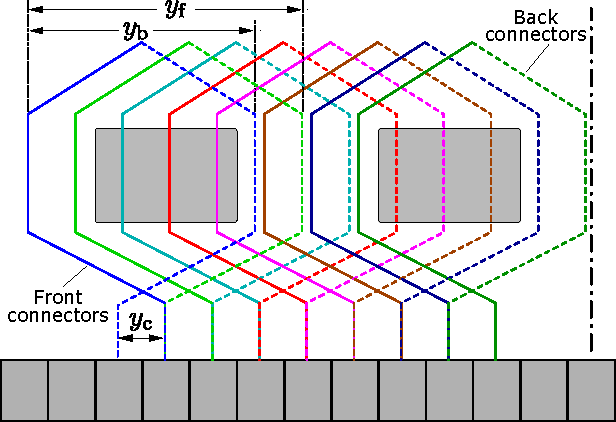
\includegraphics[width=0.85\textwidth]{fig/lec03/Lap_winding_distances_retrogressive.pdf}
				\caption{Lap winding with a retrogressive scheme (adapted from W.~Novender, \textit{Elektrische Maschinen}, Technische Hochschule Mittelhessen, 2023)}
				\label{fig:Lap_winding_distances_retrogressive}
			\end{figure}
		\end{column}
		\end{columns}
\end{frame}


%%%%%%%%%%%%%%%%%%%%%%%%%%%%%%%%%%%%%%%%%%%%%%%%%%%%%%%%%%%%%
%% Lap winding %%
%%%%%%%%%%%%%%%%%%%%%%%%%%%%%%%%%%%%%%%%%%%%%%%%%%%%%%%%%%%%%
\begin{frame}
	\frametitle{Lap winding: final remarks and single pole pair example}
	\begin{columns}
		\begin{column}{0.35\textwidth}
			\begin{itemize}
				\item Armature turns per pole: $N_\mathrm{p} = \frac{KN_\mathrm{c}}{2p}$
				\item Current per armature conductor: $I_\mathrm{c} = \frac{I_\mathrm{a}}{2 p}$
			\end{itemize}
			\onslide<2->{\begin{varblock}{Parallel connection of poles}
				For $p>1$ the lap winding parallels the armature coils for each pole enabling a higher current (but limited voltage) rating.
			\end{varblock}}%
		\end{column}
		\hfill
		\begin{column}{0.65\textwidth}
			\begin{figure}
				\centering
				\includegraphics[width=0.95\textwidth]{fig/lec03/Lap_winding.pdf}
				\caption{Lap winding with commutator unrolled along the circumferential coordinate}
			\end{figure}
		\end{column}
	\end{columns}
\end{frame}

%%%%%%%%%%%%%%%%%%%%%%%%%%%%%%%%%%%%%%%%%%%%%%%%%%%%%%%%%%%%%
%% Wave winding characteristics %%
%%%%%%%%%%%%%%%%%%%%%%%%%%%%%%%%%%%%%%%%%%%%%%%%%%%%%%%%%%%%%
\begin{frame}
	\frametitle{Wave winding characteristics}
    \begin{columns}
		\begin{column}{0.42\textwidth}
            \begin{itemize}
				\item Commutator pitch (wave winding): $y_\mathrm{c} = y_\mathrm{f} + y_\mathrm{b}$, i.e., each coil spans (nearly) the entire pole pitch.  
			\end{itemize}
			\vspace{-0.4cm}
			\onslide<2->{\begin{varblock}{Progressive winding}
				\figref{fig:Wave_winding_distances} shows a progressive winding layout since each new wave winding coil starts one commutator element to the right. 
			\end{varblock}}
		\end{column}
        \hfill
		\begin{column}{0.55\textwidth}
			\begin{figure}
				\centering
				\includegraphics[width=0.85\textwidth]{fig/lec03/Wave_winding_distances.pdf}
				\caption{Distance definitions of the armature wave winding (adapted from W.~Novender, \textit{Elektrische Maschinen}, Technische Hochschule Mittelhessen, 2023)}
				\label{fig:Wave_winding_distances}
			\end{figure}
		\end{column}
		\end{columns}
\end{frame}

%%%%%%%%%%%%%%%%%%%%%%%%%%%%%%%%%%%%%%%%%%%%%%%%%%%%%%%%%%%%%
%% Wave winding %%
%%%%%%%%%%%%%%%%%%%%%%%%%%%%%%%%%%%%%%%%%%%%%%%%%%%%%%%%%%%%%
\begin{frame}
	\frametitle{Wave winding: final remarks and single pole pair example}
	\begin{columns}
		\begin{column}{0.35\textwidth}
			\begin{itemize}
				\item Armature turns per pole: $N_\mathrm{p} = \frac{K N_\mathrm{c}}{2}$
				\item Current per armature conductor: $I_\mathrm{c} = \frac{I_\mathrm{a}}{2}$
			\end{itemize}
			\onslide<2->{\begin{varblock}{Series connection of poles}
				For $p>1$ the wave winding connects the armature coils for all poles in series enabling a higher voltage (but limited current) rating.
			\end{varblock}}
		\end{column}
		\hfill
		\begin{column}{0.65\textwidth}
			\begin{figure}
				\centering
				\includegraphics[width=0.95\textwidth]{fig/lec03/Wave_winding.pdf}
				\caption{Wave winding with commutator unrolled along the circumferential coordinate}
			\end{figure}
		\end{column}
	\end{columns}
\end{frame}

%%%%%%%%%%%%%%%%%%%%%%%%%%%%%%%%%%%%%%%%%%%%%%%%%%%%%%%%%%%%%
%% Lap and wave winding comparison %%
%%%%%%%%%%%%%%%%%%%%%%%%%%%%%%%%%%%%%%%%%%%%%%%%%%%%%%%%%%%%%
\begin{frame}
	\frametitle{Lap and wave winding comparison}
	Introducing the parameter 
	\begin{equation}
		a = \mbox{Number of parallel armature conductors}
		\label{eq:Parallel_conductors}
	\end{equation}
	we can wrap up the following summary:\pause
	\begin{equation}
		\mbox{Current per conductor: } I_\mathrm{c} = \frac{I_\mathrm{a}}{2 a}, \quad \mbox{Armature turns per pole: } N_\mathrm{p} = \frac{K N_\mathrm{c}}{2 a}.
	\end{equation}\pause
	\begin{varblock}{Comparison}
		\begin{itemize}
			\item Lap winding: $a = p$ (parallel connection of poles)
			\item Wave winding: $a = 1$ (series connection of poles)
		\end{itemize}
	\end{varblock}
\end{frame}

%%%%%%%%%%%%%%%%%%%%%%%%%%%%%%%%%%%%%%%%%%%%%%%%%%%%%%%%%%%%%
%% Commutation process %%
%%%%%%%%%%%%%%%%%%%%%%%%%%%%%%%%%%%%%%%%%%%%%%%%%%%%%%%%%%%%%
\begin{frame}
	\frametitle{Commutation process}
	During the commutation time $T_\mathrm{c}$ the brush bridges two commutator segments and the short-circuited conductor coil current $i_\mathrm{c}$ is changing signs. Here, two major scenarios can be distinguished:
	\begin{itemize}
		\item The commutation is such fast that high local current densities are prevented.
		\item The commutation is slow and high local current densities lead to sparking effects.
	\end{itemize}
    \begin{figure}
        \centering
        \includegraphics[width=0.75\textwidth]{fig/lec03/Commutation_process_time_trajectory.pdf}
        \caption{Left: simplified equivalent circuit diagram of the short-circuited coil during commutation. Right: qualitative trajectories of the conductor current $i_\mathrm{c}$} 
		\label{fig:Commutation_process_time_trajectory}
    \end{figure}
\end{frame}

%%%%%%%%%%%%%%%%%%%%%%%%%%%%%%%%%%%%%%%%%%%%%%%%%%%%%%%%%%%%%
%% Commutation process %%
%%%%%%%%%%%%%%%%%%%%%%%%%%%%%%%%%%%%%%%%%%%%%%%%%%%%%%%%%%%%%
\begin{frame}
	\frametitle{Commutation process (cont.)}
	\begin{columns}
		\begin{column}{0.4\textwidth}
			\begin{figure}
				\centering
				\includegraphics[width=0.95\textwidth]{fig/lec03/Commutator_sparking.jpg}
				\caption{Commutator sparking of a simple DC machine (source: \href{https://commons.wikimedia.org/wiki/File:Bürstenfeuer_eines_einfachen_Elektromotors.JPG}{Wikimedia Commons}, M. Frey, \href{https://creativecommons.org/licenses/by-sa/4.0/deed.den}{CC BY-SA 4.0})} 
				\label{fig:Commutator_sparking}
			\end{figure}
		\end{column}
		\begin{column}{0.6\textwidth}
			Assuming that the brush width $w_\mathrm{b}$ is much bigger than one commutator segment (which is usual practice), the commutation time $T_\mathrm{c}$ is given by
			\begin{equation}
				T_\mathrm{c} \approx \frac{w_\mathrm{b}}{v_\mathrm{c}}.
			\end{equation}
			Here, $v_\mathrm{c}$ is the brush velocity
			\begin{equation}
				v_\mathrm{c} = \omega \frac{d_\mathrm{a}}{2}
			\end{equation}
			with the armature angular velocity $\omega$ and the armature diameter $d_\mathrm{a}$. Due to the changing current in the short-circuited coil, the so-called reactane voltage $u_\mathrm{r}$ is induced:
			\begin{equation}
				u_\mathrm{r} = L_\mathrm{c} \frac{\mathrm{d}i_\mathrm{c}}{\mathrm{d}t} \approx L_\mathrm{c} \frac{i_\mathrm{a}}{a T_\mathrm{c}}.
			\end{equation}
		\end{column}
	\end{columns}
    
\end{frame}

%%%%%%%%%%%%%%%%%%%%%%%%%%%%%%%%%%%%%%%%%%%%%%%%%%%%%%%%%%%%%
%% Air gap field %%
%%%%%%%%%%%%%%%%%%%%%%%%%%%%%%%%%%%%%%%%%%%%%%%%%%%%%%%%%%%%%
\begin{frame}
	\frametitle{Air gap field}
	\begin{columns}
		\begin{column}{0.65\textwidth}
			\textbf{Assumption}: The air gap field distribution is homogenous and without any leakage (cf. \figref{fig:Ideal_air_gap_field}).\\ \onslide<2->{Consequently, we model the magnetic machine behavior with the simplified network shown in \figref{fig:Simplified_magnetic_network_DC_machine}.}% 
			\begin{figure}
				\centering
				\includegraphics[width=0.4\textwidth]{fig/lec03/Ideal_air_gap_field.pdf}
				\caption{Idealized field lines (adapted from W.~Novender, \textit{Elektrische Maschinen}, Technische Hochschule Mittelhessen, 2023)}
				\label{fig:Ideal_air_gap_field}
			\end{figure}
		\end{column}
		\hfill
		\begin{column}{0.33\textwidth}
			\onslide<2->{\begin{figure}
				\centering
				\includegraphics[height=0.65\textheight]{fig/lec03/Simplified_magnetic_network_DC_machine.pdf}
				\caption{Simplified magnetic network of a DC machine}
				\label{fig:Simplified_magnetic_network_DC_machine}
			\end{figure}}%
		\end{column}
	\end{columns}
\end{frame}

%%%%%%%%%%%%%%%%%%%%%%%%%%%%%%%%%%%%%%%%%%%%%%%%%%%%%%%%%%%%%
%% Air gap field (cont.) %%
%%%%%%%%%%%%%%%%%%%%%%%%%%%%%%%%%%%%%%%%%%%%%%%%%%%%%%%%%%%%%
\begin{frame}
	\frametitle{Air gap field (cont.)}
	\begin{columns}
		\begin{column}{0.65\textwidth}
			We introduce the following magnetic reluctances
			\begin{equation}
				\begin{alignedat}{2}
					R_\mathrm{s} &= \frac{l_\mathrm{s}}{\mu_{\mathrm{r, Fe}} \mu_0  A_\mathrm{s}} \quad  &&(\mbox{stator reluctance}), \\ \quad R_\mathrm{a} &= \frac{l_\mathrm{a}}{\mu_{\mathrm{r, Fe}}\mu_0  A_\mathrm{a}} \quad  &&(\mbox{armature reluctance}), \\
					R_\delta &= \frac{\delta}{\mu_0 A_\delta} \quad  &&(\mbox{air gap reluctance}).
				\end{alignedat}
			\end{equation}
			Above $l_i$ and $A_i$ are the respective lengths and cross-sectional areas of the field paths while $\delta$ is the air gap width. \onslide<2->{Furthermore, we have 
			$$ \mu_{\mathrm{r},\delta} = 1, \qquad \mu_{\mathrm{r, Fe}} >> 1 .$$}%
		\end{column}
		\hfill
		\begin{column}{0.35\textwidth}
			\begin{figure}
				\centering
				\includegraphics[height=0.65\textheight]{fig/lec03/Simplified_magnetic_network_DC_machine.pdf}
			\end{figure}
		\end{column}
	\end{columns}
\end{frame}

%%%%%%%%%%%%%%%%%%%%%%%%%%%%%%%%%%%%%%%%%%%%%%%%%%%%%%%%%%%%%
%% Air gap field (cont.) %%
%%%%%%%%%%%%%%%%%%%%%%%%%%%%%%%%%%%%%%%%%%%%%%%%%%%%%%%%%%%%%
\begin{frame}
	\frametitle{Air gap field (cont.)}
	\begin{columns}
		\begin{column}{0.65\textwidth}
			With $N_\mathrm{f}$ field winding turns and the field current $I_\mathrm{f}$, the air gap flux is given by:
			\begin{equation}
				\begin{split}
				\phi_\delta &= \frac{N_\mathrm{f} I_\mathrm{f}}{2 R_\delta + R_\mathrm{a} + \frac{1}{2}R_\mathrm{s}}\\
							& = \frac{N_\mathrm{f} I_\mathrm{f}}{\mu_0}\left(2\frac{\delta}{A_\delta} + \frac{l_\mathrm{a}}{\mu_{\mathrm{r, Fe}} A_\mathrm{a}} + \frac{1}{2}\frac{l_\mathrm{s}}{\mu_{\mathrm{r, Fe}} A_\mathrm{s}}\right)^{-1}. 
			\end{split}
			\label{eq:Air_gap_flux_DC_machine_simple}
			\end{equation}
			\onslide<2->{While the relative permeability of the iron paths is depending on the magnetic flux ($\mu_{\mathrm{r, Fe}} = \mu_{\mathrm{r, Fe}}(\phi)$) due to saturation (cf. \figref{fig:Permeability_of_ferromagnet}) rendering \eqref{eq:Air_gap_flux_DC_machine_simple} a nonlinear equation, we will assume that the air gap reluctance is dominating 
			\begin{equation}
				 R_\delta >> \left\{R_\mathrm{a}, R_\mathrm{s} \right\} .
				 \label{eq:DC_flux_reluctance_simpl}
			\end{equation}}%
		\end{column}
		\hfill
		\begin{column}{0.35\textwidth}
			\begin{figure}
				\centering
				\includegraphics[height=0.65\textheight]{fig/lec03/Simplified_magnetic_network_DC_machine.pdf}
			\end{figure}
		\end{column}
	\end{columns}
\end{frame}

%%%%%%%%%%%%%%%%%%%%%%%%%%%%%%%%%%%%%%%%%%%%%%%%%%%%%%%%%%%%%
%% Air gap field (cont.) %%
%%%%%%%%%%%%%%%%%%%%%%%%%%%%%%%%%%%%%%%%%%%%%%%%%%%%%%%%%%%%%
\begin{frame}
	\frametitle{Air gap field (cont.)}
	Based on \eqref{eq:Air_gap_flux_DC_machine_simple} together with \eqref{eq:DC_flux_reluctance_simpl} we can simplify the effective air gap flux to
	\begin{equation}
		\phi_\delta = \frac{N_\mathrm{f} I_\mathrm{f}}{2 R_\delta} = \frac{N_\mathrm{F} I_\mathrm{f}}{2 \frac{\delta}{\mu_0 A_\delta}} = \frac{\mu_0 N_\mathrm{f} A_\delta}{2 \delta} I_\mathrm{f}.
		\label{eq:Air_gap_flux_DC_machine}
	\end{equation}\pause
	Here, $\delta$ is the air gap width and $A_\delta$ the effective cross-sectional area of the air gap which is
	\begin{equation}
		A_\delta = \alpha p \tau_\mathrm{p} l_z .
		\label{eq:Air_gap_area_DC_machine}
	\end{equation}\pause
	Above, the following assumptions and definitions are made:
	\begin{itemize}
		\item $l_z$ is the axial length of the machine. \pause
		\item The air gap width is very small such that the pole pitch $\tau_\mathrm{p}$ can be used as a good approximation for the air gap  circumference. \pause
		\item $\alpha$ is the pole coverage, that is, the ratio of the active pole surfaces to the pole pitch (cf. \figref{fig:Magnetic_field_normal_component_DC_machine} on next slide) representing the average field density in the air gap.
	\end{itemize}
\end{frame}

%%%%%%%%%%%%%%%%%%%%%%%%%%%%%%%%%%%%%%%%%%%%%%%%%%%%%%%%%%%%%
%% Air gap field (cont.) %%
%%%%%%%%%%%%%%%%%%%%%%%%%%%%%%%%%%%%%%%%%%%%%%%%%%%%%%%%%%%%%
\begin{frame}
	\frametitle{Air gap field (cont.)}
    \begin{figure}
        \centering
        \includegraphics[height=0.67\textheight]{fig/lec03/Magnetic_field_normal_component_DC_machine.pdf}
        \caption{Principle magnetic field paths through stator and rotor as well as the (idealized) normal component of the magnetic field density $B_\delta$ in the air gap  (inspired from A. Binder, \textit{Elektrische Maschinen und Antriebe}, Vol. 2, Springer, 2017)}
		\label{fig:Magnetic_field_normal_component_DC_machine}
    \end{figure}
\end{frame}

%%%%%%%%%%%%%%%%%%%%%%%%%%%%%%%%%%%%%%%%%%%%%%%%%%%%%%%%%%%%%
%% Torque %%
%%%%%%%%%%%%%%%%%%%%%%%%%%%%%%%%%%%%%%%%%%%%%%%%%%%%%%%%%%%%%
\begin{frame}
	\frametitle{Torque}
	\begin{columns}
	\begin{column}{0.45\textwidth}
    From \eqref{eq:Air_gap_flux_DC_machine} we can calculate the air gap flux density $B_\delta$ per pole pair as
	\begin{equation}
		B_\delta = \frac{\phi_\delta}{A_\delta} = \frac{\mu_0 N_\mathrm{f}}{2 \delta p} I_\mathrm{f}.
		\label{eq:Air_gap_flux_density_DC_machine}
	\end{equation}\pause
	Assuming that the magnetic field only flows through each armature conductor in a north-south direction per pole (cf. \figref{fig:DC_machine_cross_section_force_torque}), the absolute Lorentz force per armature conductor is resulting in
	\begin{equation}
		F_\mathrm{c} =  B_\delta l_z I_\mathrm{c}= \frac{\mu_0 N_\mathrm{f} l_z}{4 \delta p a}I_\mathrm{f} I_\mathrm{a}.
		\label{eq:Lorentz_force_DC_machine_conductor}
	\end{equation}
\end{column}
\hfill
\begin{column}{0.55\textwidth}
	\begin{figure}
		\centering
		\includegraphics[width=0.725\textwidth]{fig/lec03/DC_machine_cross_section_force_torque.pdf}
		\caption{Simplified DC machine cross section with exemplary armature conductor force representation (adapted from J.~B\"ocker, \textit{Elektrische Antriebstechnik}, Paderborn University, 2020)}
		\label{fig:DC_machine_cross_section_force_torque}
	\end{figure}
\end{column}
\end{columns}
\end{frame}

%%%%%%%%%%%%%%%%%%%%%%%%%%%%%%%%%%%%%%%%%%%%%%%%%%%%%%%%%%%%%
%% Torque (cont.)%%
%%%%%%%%%%%%%%%%%%%%%%%%%%%%%%%%%%%%%%%%%%%%%%%%%%%%%%%%%%%%%
\begin{frame}
	\frametitle{Torque (cont.)}
	The torque per conductor for an armature diameter $d_\mathrm{a}$ with the conductor's radial position $\varepsilon$ is
	\begin{equation}
		T_\mathrm{c} = F_\mathrm{c} \frac{d_\mathrm{a}}{2}\sin(\varepsilon) = \frac{\mu_0 N_\mathrm{f} l_z d_\mathrm{a}}{8 \delta p a} \sin(\varepsilon) I_\mathrm{f} I_\mathrm{a}.
		\label{eq:Torque_DC_machine_conductor}
	\end{equation} \pause
	The resulting (average) machine torque $T$ for $N_\mathrm{a}$ armature conductor loops from which an $\alpha$  share is covered by the poles (cf. \figref{fig:Magnetic_field_normal_component_DC_machine}) is
	\begin{equation}
		\begin{split}
			T 	&= 2 \alpha N_\mathrm{a} \frac{1}{\pi} \int_0^\pi T_\mathrm{c} \mathrm{d}\varepsilon \\ 
				&= \frac{\mu_0 \alpha N_\mathrm{f} N_\mathrm{a} l_z d_\mathrm{a}}{4 \delta p a} I_\mathrm{f} I_\mathrm{a} \int_0^\pi \sin(\varepsilon) \mathrm{d}\varepsilon \\ 
				&=\frac{\mu_0 \alpha N_\mathrm{f} N_\mathrm{a} l_z d_\mathrm{a}}{4 \delta p a \pi} I_\mathrm{f} I_\mathrm{a} \left[-\cos(\varepsilon)\right]_0^\pi\\
				& = \frac{\mu_0 \alpha N_\mathrm{f} N_\mathrm{a} l_z d_\mathrm{a}}{2 \delta p a \pi} I_\mathrm{f} I_\mathrm{a}.
		\end{split}
	\end{equation}
\end{frame}

%%%%%%%%%%%%%%%%%%%%%%%%%%%%%%%%%%%%%%%%%%%%%%%%%%%%%%%%%%%%%
%% Torque (cont.)%%
%%%%%%%%%%%%%%%%%%%%%%%%%%%%%%%%%%%%%%%%%%%%%%%%%%%%%%%%%%%%%
\begin{frame}
	\frametitle{Torque (cont.)}
	With $\tau_\mathrm{p} = \pi d_\mathrm{s}/(2 p) = \pi d_\mathrm{a}/(2 p)$ assuming a very small air gap width $\delta$ (cf. \figref{fig:DC_machine_cross_section_two_pole_pairs}) we can also rewrite the torque as
	\begin{equation}
		\begin{split}
		T &= \frac{\mu_0 \alpha N_\mathrm{f} N_\mathrm{a} l_z d_\mathrm{a}}{2 \delta p a \pi} I_\mathrm{f} I_\mathrm{a}\\
		&= \frac{\mu_0 \alpha N_\mathrm{f} N_\mathrm{a} l_z \tau_\mathrm{p}}{\pi^2  \delta a} I_\mathrm{f} I_\mathrm{a}.
		\end{split}
		\label{eq:Torque_DC_machine}
	\end{equation}
	Some remarks on machine design impacts on the torque:
	\begin{itemize}
		\item To produce torque, both field current $I_\mathrm{f}$ and armature current $I_\mathrm{a}$ are required.
		\item The larger the machine dimensions (axial length $l_\mathrm{z}$ and armature diameter $d_\mathrm{a} \approx d_\mathrm{s}$), the larger the torque.
		\item The more winding turns $N_\mathrm{a}$ and $N_\mathrm{f}$, the larger the torque.
		\item The smaller the air gap width $\delta$, the larger the torque.
	\end{itemize}
\end{frame}

%%%%%%%%%%%%%%%%%%%%%%%%%%%%%%%%%%%%%%%%%%%%%%%%%%%%%%%%%%%%%
%% Effective field inductance and effective flux linkage %%
%%%%%%%%%%%%%%%%%%%%%%%%%%%%%%%%%%%%%%%%%%%%%%%%%%%%%%%%%%%%%
\begin{frame}
	\frametitle{Effective field inductance and effective flux linkage}
    To write \eqref{eq:Torque_DC_machine} more compact, we introduce the effective field inductance 
	\begin{equation}
		L_\mathrm{f}' =  \frac{\mu_0 \alpha N_\mathrm{f} N_\mathrm{a} l_z d_\mathrm{a}}{2 \delta p a \pi} = \frac{\mu_0 \alpha N_\mathrm{f} N_\mathrm{a} l_z \tau_\mathrm{p}}{\pi^2  \delta a}.
		\label{eq:Effective_field_inductance}
	\end{equation}
	Compared to the self-inductance of the field winding 
	\begin{equation}
		L_\mathrm{f} = \frac{N_\mathrm{f}^2}{2 R_\delta} = \frac{\mu  \alpha p \tau_\mathrm{p} l_z N_\mathrm{f}^2}{4 \delta},
	 \end{equation}
	 we find
	 \begin{equation}
		 L_\mathrm{f}' = \underbrace{\frac{4}{a \pi^2}\frac{N_\mathrm{a}}{N_\mathrm{f}}}_{c} L_\mathrm{f}  = c L_\mathrm{f} .
	\end{equation}
	Finally, we define the effective field flux linkage $\psi_\mathrm{f}'$ to rewrite the torque expression
	\begin{equation}
		\psi_\mathrm{f}' = L_\mathrm{f}' I_\mathrm{f}, \hspace{1cm} T = c L_\mathrm{f} I_\mathrm{f} I_\mathrm{a} = L_\mathrm{f}' I_\mathrm{f} I_\mathrm{a}  = \psi_\mathrm{f}' I_\mathrm{a}.
		\label{eq:Effective_field_flux_linkage}
	\end{equation}
\end{frame}


%%%%%%%%%%%%%%%%%%%%%%%%%%%%%%%%%%%%%%%%%%%%%%%%%%%%%%%%%%%%%
%% Induced voltage %%
%%%%%%%%%%%%%%%%%%%%%%%%%%%%%%%%%%%%%%%%%%%%%%%%%%%%%%%%%%%%%
\begin{frame}
	\frametitle{Induced voltage}
	 Still assuming the homogenous flux density from \eqref{eq:Air_gap_flux_density_DC_machine} $$B_\delta = \frac{\mu_0 N_\mathrm{f}}{2 \delta p} I_\mathrm{f},$$ we find that the magnetic flux linkage per armature conductor loop is
	\begin{equation}
		\psi_\mathrm{c} = A_\mathrm{c}B_\delta= l_\mathrm{z} d_\mathrm{a}\cos(\varepsilon) \frac{\mu_0 N_\mathrm{f}}{2 \delta p} I_\mathrm{f}.
		\label{eq:Magnetic_flux_linkage_per_conductor}
	\end{equation}
	Above, $A_\mathrm{c}$ is the cross-sectional area of an armature conductor loop (cf. \figref{eq:Torque_DC_machine}). Assuming that the armature is rotating with the speed $n$ (or angular velocity $\omega = 2 \pi n=\dot{\varepsilon}$), the induced voltage per armature conductor loop is
	\begin{equation}
		\begin{split}
			u_\mathrm{c} &= -\frac{\mathrm{d}\psi_\mathrm{c}}{\mathrm{d}t} = -\frac{\mu_0 N_\mathrm{f} l_\mathrm{z} d_\mathrm{a}}{2 \delta p} I_\mathrm{f} \frac{\mathrm{d}}{\mathrm{d}t} \cos(\varepsilon)\\
			&= \frac{\mu_0 N_\mathrm{f} l_\mathrm{z} d_\mathrm{a}}{2 \delta p} I_\mathrm{f} \omega \sin(\varepsilon).
		\end{split}
		\label{eq:Induced_voltage_per_conductor}
	\end{equation}
\end{frame}

%%%%%%%%%%%%%%%%%%%%%%%%%%%%%%%%%%%%%%%%%%%%%%%%%%%%%%%%%%%%%
%% Induced voltage %%
%%%%%%%%%%%%%%%%%%%%%%%%%%%%%%%%%%%%%%%%%%%%%%%%%%%%%%%%%%%%%
\begin{frame}
	\frametitle{Induced voltage (cont.)}
	 To calculate the total induced voltage $u_\mathrm{i}$, we integrate \eqref{eq:Induced_voltage_per_conductor} over all armature conductor loops considering 
	 \begin{itemize}
		\item $N_\mathrm{a}$ total armature conductor loops,
		\item $2 a$ parallel armature conductors per pole pair (depends on winding scheme, cf. \eqref{eq:Parallel_conductors}),
		\item $\alpha$ ratio of effective pole coverage,
	 \end{itemize}
	 resulting in:
	 \begin{equation}
		 \begin{split}
			 u_\mathrm{i} &= \frac{N_\mathrm{a}\alpha}{2 a} \frac{1}{\pi} \int_0^\pi u_\mathrm{c} \mathrm{d}\varepsilon
			 = \omega I_\mathrm{f}\frac{\mu_0 N_\mathrm{f} N_\mathrm{a} l_\mathrm{z} d_\mathrm{a} }{4 \delta p a \pi} \int_0^\pi \sin(\varepsilon) \mathrm{d}\varepsilon
			 = \omega I_\mathrm{f}\frac{\mu_0 N_\mathrm{f} N_\mathrm{a} l_\mathrm{z} d_\mathrm{a} }{4 \delta p a \pi} \left[-\cos(\varepsilon)\right]_0^\pi\\
			 &= \omega I_\mathrm{f}\frac{\mu_0 N_\mathrm{f} N_\mathrm{a} l_\mathrm{z} d_\mathrm{a}}{2 \delta p a \pi} = \omega I_\mathrm{f}\frac{\mu_0 N_\mathrm{f} N_\mathrm{a} l_\mathrm{z} \tau_p}{ \pi^2 \delta a } = \omega I_\mathrm{f} L_\mathrm{f}' = \omega  \psi_\mathrm{f}'.
		 \end{split}
	 \end{equation}
\end{frame}

%%%%%%%%%%%%%%%%%%%%%%%%%%%%%%%%%%%%%%%%%%%%%%%%%%%%%%%%%%%%%
%% Equivalent circuit diagram and summary of important equations %%
%%%%%%%%%%%%%%%%%%%%%%%%%%%%%%%%%%%%%%%%%%%%%%%%%%%%%%%%%%%%%
\begin{frame}
	\frametitle{Equivalent circuit diagram and summary of important equations}
	\begin{columns}
		\begin{column}{0.55\textwidth}
	Field and armature voltage equations:
	\begin{equation}
		\begin{aligned}
			u_\mathrm{f} &= R_\mathrm{f} i_\mathrm{f} + L_\mathrm{f} \frac{\mathrm{d}i_\mathrm{f}}{\mathrm{d}t} \\
			u_\mathrm{a} &= R_\mathrm{a} i_\mathrm{a} + L_\mathrm{a} \frac{\mathrm{d}i_\mathrm{a}}{\mathrm{d}t} + u_\mathrm{i} + u_\mathrm{b}
		\end{aligned}
	\end{equation}
	Induced voltage:
	\begin{equation*}
			u_\mathrm{i} = \omega \psi_\mathrm{f}' = \omega I_\mathrm{f} L_\mathrm{f}' 
	\end{equation*}
	Torque:
	\begin{equation*}
		T =  L_\mathrm{f}' i_\mathrm{f} i_\mathrm{a}  = \psi_\mathrm{f}' i_\mathrm{a}
	\end{equation*}
	\textbf{Note}: we represent the machine currents with small letters to indicate that they are time-dependent (e.g., if the external voltage supplied is varying).
\end{column}
\hfill
\begin{column}{0.45\textwidth}
	\begin{figure}
		\centering
		\includegraphics[width=0.8\textwidth]{fig/lec03/ECD_DC_machine.pdf}
		\caption{Equivalent circuit diagram of the DC machine}
		\label{fig:ECD_DC_machine}
	\end{figure}
\end{column}
\end{columns}
\end{frame}

%%%%%%%%%%%%%%%%%%%%%%%%%%%%%%%%%%%%%%%%%%%%%%%%%%%%%%%%%%%%%
%% Intermediate remarks on the DC machine model %%
%%%%%%%%%%%%%%%%%%%%%%%%%%%%%%%%%%%%%%%%%%%%%%%%%%%%%%%%%%%%%
\begin{frame}
	\frametitle{Intermediate remarks on the DC machine model} 
	During the derivation of the DC machine model, we made several assumptions:
	\begin{itemize}
		\item The air gap magnetic field is homogenous and without any leakage.
		\item The air gap reluctance is dominating the magnetic circuit (neglecting the iron path reluctances including potential magnetic saturation).
		\item The magnetic field lines follow distinct paths through the armature winding.
		\item There is no mutual inductance between the stator and rotor (ideal orthogonal windings).
		\item The magnetic field in the air gap and in the armature is governed by the field winding current only (that is, we have neglected the armature current impact on the field).
	\end{itemize}
	\begin{varblock}{Model accuracy}
		We represent the DC machine by a time-invariant, lumped-parameter model which is based on several substantial simplifications. While this model is likely sufficient for many applications, systematic deviations between the observed behavior of real machines and the model predictions are to be expected.
	\end{varblock}
\end{frame} % DC machines
\part{Transformers}
\title{Transformers}  
\date{}  
\frame{\titlepage} 

%%%%%%%%%%%%%%%%%%%%%%%%%%%%%%%%%%%%%%%%%%%%%%%%%%%%%%%%%%%%%
%% Transformer definition %%
%%%%%%%%%%%%%%%%%%%%%%%%%%%%%%%%%%%%%%%%%%%%%%%%%%%%%%%%%%%%%
\begin{frame}
	\frametitle{Transformer definition}
    \begin{columns}
		\begin{column}{0.65\textwidth}
            \begin{varblock}{Transformer}
                A transformer is a static device that transfers electrical energy between two or more circuits through electromagnetic induction. It converts the AC voltage levels between inputs and outputs.   
            \end{varblock}
            \begin{itemize}
                \item<2-> While a transformer is sometimes called a ``static~machine'', it does not meet the formal definition of an electrical machine (compare first chapter).
                \item<3-> However, transformers share some working principles with electrical machines and are also often used as components of electrical power systems including drives.
            \end{itemize}
		\end{column}
        \hfill
		\begin{column}{0.35\textwidth}
			\onslide<1->
			\begin{figure}
				\centering
				\includegraphics[width=0.75\textwidth]{fig/lec04/Transformer_rural_pole.jpg}
				\caption{Transformer integrated at a utility pole (source: \href{https://pxhere.com/en/photo/795672}{pxhere.com}, public domain)}
			\end{figure}
		\end{column}
		\end{columns}
\end{frame}

%%%%%%%%%%%%%%%%%%%%%%%%%%%%%%%%%%%%%%%%%%%%%%%%%%%%%%%%%%%%%
%% Examples of transformers %%
%%%%%%%%%%%%%%%%%%%%%%%%%%%%%%%%%%%%%%%%%%%%%%%%%%%%%%%%%%%%%
\begin{frame}
	\frametitle{Examples of transformers}
	\begin{figure}
		\centering
		\begin{subfigure}[b]{0.49\textwidth}
			\centering
			\includegraphics[width=0.45\textwidth]{fig/lec04/Power_supply_transformer.jpg}
			\caption{Power supply transformer (source: \href{https://commons.wikimedia.org/wiki/File:Philips_N4422_-_power_supply_transformer-2098.jpg}{Wikimedia Commons}, R.~Spekking, \href{https://creativecommons.org/licenses/by-sa/4.0/deed}{CC BY-SA 4.0})}
		\end{subfigure}
		\hfill
		\begin{subfigure}[b]{0.49\textwidth}
			\centering
			\includegraphics[width=0.45\textwidth]{fig/lec04/Single_phase_transformer.jpg}
			\caption{Single-phase transformer (source: \href{https://commons.wikimedia.org/wiki/File:DB_Unterwerk_Güsen,_Trafo_p.jpg}{Wikimedia Commons}, Georg, \href{https://creativecommons.org/licenses/by-sa/4.0/deed.en}{CC BY-SA 4.0})}
		\end{subfigure}
		\\
		\begin{subfigure}[b]{0.49\textwidth}
			\centering
			\includegraphics[width=0.45\textwidth]{fig/lec04/Three_phase_transformer.jpg}
			\caption{Three-phase transformer (source: \href{https://commons.wikimedia.org/wiki/File:Dornbirn-Umspannwerk_Werben-110kV_FS6-Anlage_Trafo_Elin_220-110kV-01ASD.jpg}{Wikimedia Commons}, Asurnipal, \href{https://creativecommons.org/licenses/by-sa/4.0/deed.en}{CC BY-SA 4.0})}
		\end{subfigure}
		\hfill
		\begin{subfigure}[b]{0.49\textwidth}
			\centering
			\includegraphics[width=0.45\textwidth]{fig/lec04/Tapped_transformer.jpg}
			\caption{Variable tapped transformer (source: \href{https://commons.wikimedia.org/wiki/File:Variable-tap_regulating_transformer_(Rankin_Kennedy,_Electrical_Installations,_Vol_II,_1909).jpg}{Wikimedia Commons}, public domain)}
		\end{subfigure}
		\caption*{Examples of transformers} 
        \label{fig:examples_transformers}
	\end{figure}
\end{frame}

%%%%%%%%%%%%%%%%%%%%%%%%%%%%%%%%%%%%%%%%%%%%%%%%%%%%%%%%%%%%%
%% Electromagnetic modeling of the single-phase transformer %%
%%%%%%%%%%%%%%%%%%%%%%%%%%%%%%%%%%%%%%%%%%%%%%%%%%%%%%%%%%%%%
\begin{frame}
	\frametitle{Electromagnetic modeling of the single-phase transformer}
    \begin{columns}
		\begin{column}{0.45\textwidth}
            Recap from \eqref{eq:flux_linkage_matrix_transformer}: for some given current $\bm{i}$, the flux linkages $\bm{\psi}$ in the transformer windings are
			\begin{equation*}
				\bm{\psi} = \begin{bmatrix} \psi_1 \\ \psi_2 \end{bmatrix} = \begin{bmatrix} L_1 & M \\ M & L_2 \end{bmatrix} \begin{bmatrix} i_1 \\ i_2 \end{bmatrix} = \bm{L}\bm{i}
			\end{equation*}
			where $L_1$ and $L_2$ are the self-inductances of the primary and secondary winding, respectively, and $M$ is the mutual inductance.
			\\[1em] \pause
			Note: The above equation is an algebraic relation, that is, it is valid for any time instant $t$ and applies to both AC and DC excitation of the transformer. 
		\end{column}
        \hfill
		\begin{column}{0.525\textwidth}
			\onslide<1->
			\begin{figure}
				\centering
				\includegraphics[height=0.575\textheight]{fig/lec02/Transformer3d_col3.pdf}
			\end{figure}
		\end{column}
		\end{columns}
\end{frame}

%%%%%%%%%%%%%%%%%%%%%%%%%%%%%%%%%%%%%%%%%%%%%%%%%%%%%%%%%%%%%
%% Dynamic modeling of the single-phase transformer %%
%%%%%%%%%%%%%%%%%%%%%%%%%%%%%%%%%%%%%%%%%%%%%%%%%%%%%%%%%%%%%
\begin{frame}
	\frametitle{Dynamic modeling of the single-phase transformer}
		The dynamic transformer behavior can be represented by the ECD in \figref{fig:General_transformer_ECD}, which also considers the internal resistances of the windings. Applying Faraday's law, the resulting differential equations are:
		\begin{align}
			u_1(t) = R_1 i_1(t) + \frac{\mathrm{d}\psi_1(t)}{\mathrm{d}t}, \qquad u_2(t) = R_2 i_2(t) + \frac{\mathrm{d}\psi_2(t)}{\mathrm{d}t}. \label{eq:transformer_differential_equations}
		\end{align} \pause
		Inserting \eqref{eq:flux_linkage_matrix_transformer} delivers:
		\begin{align}
			u_1(t) = R_1 i_1(t) + L_1 \frac{\mathrm{d}i_1(t)}{\mathrm{d}t} + M \frac{\mathrm{d}i_2(t)}{\mathrm{d}t}, \qquad
			u_2(t) = R_2 i_2(t) + L_2 \frac{\mathrm{d}i_2(t)}{\mathrm{d}t} + M \frac{\mathrm{d}i_1(t)}{\mathrm{d}t}. \label{eq:transformer_differential_equations_2}
		\end{align}
\begin{figure}
\onslide<1->
\begin{columns}
	\begin{column}{0.55\textwidth}
            \centering
            \includegraphics[width=0.8\textwidth]{fig/lec04/General_transformer_ECD.pdf}
    \end{column}
    \begin{column}{0.45\textwidth}
        \caption{\raggedright General equivalent circuit diagram (ECD) of a transformer (note: that both ports of the transformer are denoted in the load convention reference frame which is an arbitrary representation decision).}
		\label{fig:General_transformer_ECD}
    \end{column}
\end{columns}
\end{figure}
\end{frame}

%%%%%%%%%%%%%%%%%%%%%%%%%%%%%%%%%%%%%%%%%%%%%%%%%%%%%%%%%%%%%
%% Dynamic modeling of the single-phase transformer (cont.) %%
%%%%%%%%%%%%%%%%%%%%%%%%%%%%%%%%%%%%%%%%%%%%%%%%%%%%%%%%%%%%%
\begin{frame}
	\frametitle{Dynamic modeling of the single-phase transformer (cont.)}
		The model \eqref{eq:transformer_differential_equations_2} can be represented by the T-type ECD in \figref{fig:Transformer_T_ECD}. It may be noted that $L_1-M$ and $L_2-M$ can have negative values due to the model representation. 
		\\[1em] \pause
		By rearranging \eqref{eq:transformer_differential_equations_2}, we can also write the dynamic transformer model in vector-matrix form:
		\begin{equation}
			\begin{bmatrix}	u_1(t)\\u_2(t) \end{bmatrix} = \bm{u}(t) = \begin{bmatrix} R_1 & 0 \\ 0 & R_2 \end{bmatrix} \begin{bmatrix} i_1(t)\\i_2(t) \end{bmatrix} + \begin{bmatrix} L_1 & M \\ M & L_2 \end{bmatrix} \frac{\mathrm{d}}{\mathrm{d}t} \begin{bmatrix} i_1(t)\\i_2(t) \end{bmatrix} = \bm{R}\bm{i}(t) + \bm{L}\frac{\mathrm{d}}{\mathrm{d}t}\bm{i}(t).  
			\label{eq:transformer_differential_equations_matrix_form}
		\end{equation}
\begin{figure}
\begin{columns}
	\onslide<1->
	\begin{column}{0.55\textwidth}
            \centering
            \includegraphics[width=0.9\textwidth]{fig/lec04/Transformer_T_ECD.pdf}
    \end{column}
    \begin{column}{0.45\textwidth}
        \caption{\raggedright T-type ECD of a transformer (note that the model \eqref{eq:transformer_differential_equations_matrix_form} assumes linear time-invariant (LTI) behavior, which among other effects neglects magnetic saturation).}
		\label{fig:Transformer_T_ECD}
    \end{column}
\end{columns}
\end{figure}
\end{frame}

%%%%%%%%%%%%%%%%%%%%%%%%%%%%%%%%%%%%%%%%%%%%%%%%%%%%%%%%%%%%%
%% Dynamic modeling of the single-phase transformer (cont.) %%
%%%%%%%%%%%%%%%%%%%%%%%%%%%%%%%%%%%%%%%%%%%%%%%%%%%%%%%%%%%%%
\begin{frame}
	\frametitle{Dynamic modeling of the single-phase transformer (cont.)}
		Rearranging \eqref{eq:transformer_differential_equations_matrix_form} gives the state-space representation of the transformer model
		\begin{equation}
			\frac{\mathrm{d}}{\mathrm{d}t}\bm{i}(t) = \bm{L}^{-1}\left(\bm{u}(t)-\bm{R}\bm{i}(t) \right)
			\label{eq:transformer_state_space_01}
		\end{equation}
		with
		$$ \renewcommand*{\arraystretch}{1.3} \bm{L}^{-1} = \frac{1}{L_1L_2 - M^2} \begin{bmatrix} L_2 & -M \\ -M & L_1 \end{bmatrix} = \frac{1}{\sigma} \begin{bmatrix} \frac{1}{L_1} &  \frac{-M}{L_1 L_2} \\ \frac{-M}{L_1 L_2} & \frac{1}{L_2} \end{bmatrix}.$$
		\pause
		Above, $\sigma$ is the leakage coefficient defined as (compare also \eqref{eq:coupling_coefficient})
		\begin{equation}
			\sigma = \frac{L_1 L_2 -M^2}{L_1 L_2 } = 1 - \frac{M^2}{ L_1 L_2} = 1 - k^2 .
		\end{equation}
		\pause
		Finally, the state-space representation of the transformer model (with the currents as states) is
		\begin{equation}
			\renewcommand*{\arraystretch}{1.3} 
			\frac{\mathrm{d}}{\mathrm{d}t}\bm{i}(t) = \begin{bmatrix} -\frac{R_1}{\sigma L_1} & \frac{R_2 M}{\sigma L_1 L_2} \\ \frac{R_1 M}{\sigma L_1 L_2} & -\frac{R_2}{\sigma L_2} \end{bmatrix} \bm{i}(t) + \begin{bmatrix} \frac{1}{\sigma L_1} & -\frac{M}{\sigma L_1 L_2} \\ -\frac{M}{\sigma L_1 L_2} & \frac{1}{\sigma L_2} \end{bmatrix} \bm{u}(t) = \bm{A} \bm{i}(t) + \bm{B} \bm{u}(t) .	 
			\label{eq:transformer_state_space_02}
		\end{equation}
\end{frame}

%%%%%%%%%%%%%%%%%%%%%%%%%%%%%%%%%%%%%%%%%%%%%%%%%%%%%%%%%%%%%
%% Steady-state of the single-phase transformer %%
%%%%%%%%%%%%%%%%%%%%%%%%%%%%%%%%%%%%%%%%%%%%%%%%%%%%%%%%%%%%%
\begin{frame}
	\frametitle{Steady-state modeling of the single-phase transformer}
		Assuming that the transformer operates in steady state and that all quantities are sinusoidal, the state-space model \eqref{eq:transformer_state_space_02} can be simplified and represented by complex phasors:
			$$x(t) = \hat{x} \cos(\omega_\mathrm{el} t+ \varphi_{\mathrm{x}}) = \mathrm{Re}\left\{\hat{x} e^{\iu (\omega_\mathrm{el} t + \varphi_{\mathrm{x}})}\right\}= \mathrm{Re}\left\{\underline{X} e^{\iu \omega_\mathrm{el} t}\right\}.$$
			\pause
		From \eqref{eq:transformer_differential_equations_matrix_form} we receive
		\begin{align}
			\bm{\underline{U}} = \begin{bmatrix} \underline{U}_1 \\ \underline{U}_2 \end{bmatrix} = \bm{R}\bm{\underline{I}} + \iu \omega_\mathrm{el} \bm{L}\bm{\underline{I}} = \bm{\underline{Z}}\, \bm{\underline{I} } = \begin{bmatrix} R_1 + \iu \omega_\mathrm{el} L_1 & \iu \omega_\mathrm{el} M \\ \iu \omega_\mathrm{el} M & R_2 + \iu \omega_\mathrm{el} L_2 \end{bmatrix} \begin{bmatrix} \underline{I}_1 \\ \underline{I}_2 \end{bmatrix}.
			\label{eq:transformer_steady_state_voltage_response}
		\end{align}
		\pause
		For some given $\bm{\underline{U}}$ we can calculate the current phasor $\bm{\underline{I}}$ (i.e., the steady-state current response) by solving:
		\begin{align}
			\renewcommand*{\arraystretch}{1.3} 
			\bm{\underline{I}} = \bm{\underline{Z}}^{-1} \bm{\underline{U}} .
			\label{eq:transformer_steady_state_current_response}
		\end{align}
		\pause
		Alternative scenarios can be also considered, e.g., defining $\underline{U}_1$ (input voltage) and $\underline{I}_2$ (load current) as given and solving for $\underline{I}_1$ and $\underline{U}_2$ by rearranging \eqref{eq:transformer_steady_state_voltage_response}. 
\end{frame}

%%%%%%%%%%%%%%%%%%%%%%%%%%%%%%%%%%%%%%%%%%%%%%%%%%%%%%%%%%%%%
%% Steady-state of the single-phase transformer (cont.) %%
%%%%%%%%%%%%%%%%%%%%%%%%%%%%%%%%%%%%%%%%%%%%%%%%%%%%%%%%%%%%%
\begin{frame}
	\frametitle{Steady-state modeling of the single-phase transformer (cont.)}
		Assuming that the transformer is not loaded ($I_2 = 0$) and that it is lossless ($R_1 = 0$), \eqref{eq:transformer_steady_state_voltage_response} simplifies to
		\begin{equation}
			\begin{bmatrix} \underline{U}_1 \\ \underline{U}_2 \end{bmatrix} = \begin{bmatrix} \iu \omega_\mathrm{el} L_1  \\ \iu \omega_\mathrm{el} M  \end{bmatrix} \underline{I}_1.
		\end{equation} \pause
		The voltage transformation ratio in this case results in
		\begin{equation}
			\frac{U_1}{U_2} = \frac{\iu \omega_{\mathrm{el}} L_1 I_1}{\iu \omega_{\mathrm{el}} M I_1}  = \frac{L_1}{M}.
		\end{equation}
		\pause
		Assuming further that the transformer is leakage-free ($L_{1,\sigma}=0$), the voltage transformation ratio simplifies to (compare also \eqref{eq:inductance_split})
		\begin{equation}
			\frac{U_1}{U_2} = \frac{L_1}{M} = \frac{\Lambda_{21}N_1^2}{\Lambda_{21}N_1 N_2}  = \frac{N_1}{N_2} = \ddot{u}.
			\label{eq:voltage_transformation_ratio}
		\end{equation}
		\pause
		Hence, this famous result is only valid for the abstract case of a lossless, leakage-free, and, unloaded transformer -- i.e., not applicable to real-world transformers 
\end{frame}

%%%%%%%%%%%%%%%%%%%%%%%%%%%%%%%%%%%%%%%%%%%%%%%%%%%%%%%%%%%%%
%% Transformation of the secondary side variables %%
%%%%%%%%%%%%%%%%%%%%%%%%%%%%%%%%%%%%%%%%%%%%%%%%%%%%%%%%%%%%%
\begin{frame}
	\frametitle{Transformation of the secondary side variables}
		Sometimes it can be helpful to (mathematically) transform the secondary side variables to ease the mathematical analysis. This can be done by introducing the transformation factor $\alpha$:
		\begin{equation}
			u_2' = \alpha u_2, \qquad i_2' = \frac{1}{\alpha} i_2.
		\end{equation}
		\pause
		Here, $u_2'$ and $i_2'$ are the transformed secondary side voltage and current, respectively. \pause The primary voltage equation reads
		\begin{equation}
			\begin{split}
			u_1(t) &= R_1 i_1(t) + L_1 \frac{\mathrm{d}i_1(t)}{\mathrm{d}t} + M \frac{\mathrm{d}i_2(t)}{\mathrm{d}t}  = R_1 i_1 (t)+ L_1 \frac{\mathrm{d}i_1(t)}{\mathrm{d}t}  + \alpha M \frac{\mathrm{d}i_2'(t)}{\mathrm{d}t}  \\&= R_1 i_1(t) + L_1 \frac{\mathrm{d}i_1(t)}{\mathrm{d}t} + M' \frac{\mathrm{d}i_2'(t)}{\mathrm{d}t}
		\end{split}
		\end{equation}
		with the transformed mutual inductance $M' = \alpha M$. 
\end{frame}

%%%%%%%%%%%%%%%%%%%%%%%%%%%%%%%%%%%%%%%%%%%%%%%%%%%%%%%%%%%%%
%% Transformation of the secondary side variables (cont.) %%
%%%%%%%%%%%%%%%%%%%%%%%%%%%%%%%%%%%%%%%%%%%%%%%%%%%%%%%%%%%%%
\begin{frame}
	\frametitle{Transformation of the secondary side variables (cont.)}
		Multiplying the secondary voltage equation with $\alpha$ gives 
		\begin{equation}
			\begin{split}
			\alpha  u_2(t)  &=  \alpha R_2 i_2(t) + \alpha L_2 \frac{\mathrm{d}i_2(t)}{\mathrm{d}t} + \alpha M \frac{\mathrm{d}i_1(t)}{\mathrm{d}t}\\
			\Leftrightarrow \quad u_2'(t) &= \alpha^2 R_2 i_2'(t) + \alpha^2 L_2 \frac{\mathrm{d}i_2'(t)}{\mathrm{d}t} + \alpha M \frac{\mathrm{d}i_1(t)}{\mathrm{d}t}\\
			\Leftrightarrow \quad u_2'(t) &=  R'_2 i_2'(t) + L'_2 \frac{\mathrm{d}i_2'(t)}{\mathrm{d}t} + M' \frac{\mathrm{d}i_1(t)}{\mathrm{d}t}
		\end{split}
		\label{eq:secondary_voltage_equation_transformed}
		\end{equation}
		with the transformed resistance $R'_2 = \alpha^2 R_2$ and inductance $L'_2 = \alpha^2 L_2$. 
		\pause
		\begin{figure}
			\begin{columns}
				\begin{column}{0.64\textwidth}
						\centering
						\includegraphics[width=0.99\textwidth]{fig/lec04/Transformer_T_ECD_gen_transf.pdf}
				\end{column}
				\begin{column}{0.35\textwidth}
					\caption{\raggedright T-type ECD of a transformer with transformed secondary side variables for some arbitrary transformation factor $\alpha$ (note that $k$ and $\sigma$ are transformation invariant.)}
					\label{fig:Transformer_T_ECD_gen_transf}
				\end{column}
			\end{columns}
		\end{figure}
\end{frame}

%%%%%%%%%%%%%%%%%%%%%%%%%%%%%%%%%%%%%%%%%%%%%%%%%%%%%%%%%%%%%
%% Transformation of the secondary side variables by the turn ratio %%
%%%%%%%%%%%%%%%%%%%%%%%%%%%%%%%%%%%%%%%%%%%%%%%%%%%%%%%%%%%%%
\begin{frame}
	\frametitle{Transformation of the secondary side variables by the turn ratio}
	With $$\alpha = \ddot{u} = N_1/N_2$$ being the turn ratio as the transformation factor, \pause we receive:
	\begin{equation}
		M' = (N_1/N_2)M = L_{1,\mathrm{m}}, \qquad L'_2 = (N_1^2/N_2^2) L_2
	\end{equation}
		with $L_{1,\mathrm{m}}$ being the primary magnetizing inductance, cf. \eqref{eq:inductance_split}. \pause Moreover, we have
	\begin{equation}
		L_1 - M' = L_{1,\sigma}, \qquad L_2' - M'2 =  (N_1^2/N_2^2) L_{2,\sigma} = L'_{2,
		\sigma}
	\end{equation}
	with $L_{1,\sigma}$ and $L_{2,\sigma}$ being the leakage inductances of the primary and secondary winding. \pause
	\begin{figure}
		\begin{columns}
			\begin{column}{0.64\textwidth}
					\centering
					\includegraphics[width=0.99\textwidth]{fig/lec04/Transformer_T_ECD_turn_transf.pdf}
			\end{column}
			\begin{column}{0.35\textwidth}
				\caption{\raggedright T-type ECD of a transformer with $\alpha =N_1/N_2$ (note that all inductances within this model representation have a direct physical interpretation.)}
				\label{fig:Transformer_T_ECD_turn_transf}
			\end{column}
		\end{columns}
	\end{figure}	
\end{frame}

%%%%%%%%%%%%%%%%%%%%%%%%%%%%%%%%%%%%%%%%%%%%%%%%%%%%%%%%%%%%%
%% Transformation towards a single stray inductance %%
%%%%%%%%%%%%%%%%%%%%%%%%%%%%%%%%%%%%%%%%%%%%%%%%%%%%%%%%%%%%%
\begin{frame}
	\frametitle{Transformation towards a single stray inductance}
	With $$\alpha = M/L_2$$ as the transformation factor, \pause we receive:
	\begin{equation}
		L'_2 - M' = \alpha^2 L_2 - \alpha M = L_{2,\sigma} = 0,
	\end{equation}
		that is, the secondary transformed leakage inductance is vanishing. \pause Moreover, we have
	\begin{equation}
		L_1 - M' = L'_{1,\sigma}=\sigma L_1 , \qquad M'  = M^2 / L_2.
	\end{equation} 
	\onslide<5->
	With the alternative choice $\alpha = L_1/M$, the leakage inductance gets concentrated on the secondary side (not explicitly shown).
	\begin{figure}
		\onslide<4->
		\begin{columns}
			\begin{column}{0.64\textwidth}
					\centering
					\includegraphics[width=0.99\textwidth]{fig/lec04/Transformer_T_ECD_stray_transf.pdf}
			\end{column}
			\begin{column}{0.35\textwidth}
				\caption{\raggedright T-type ECD of a transformer with $\alpha =M/L_2$}
				\label{fig:Transformer_T_ECD_stray_transf}
			\end{column}
		\end{columns}
	\end{figure}	
\end{frame}

%%%%%%%%%%%%%%%%%%%%%%%%%%%%%%%%%%%%%%%%%%%%%%%%%%%%%%%%%%%%%
%% Typical transformer core types %%
%%%%%%%%%%%%%%%%%%%%%%%%%%%%%%%%%%%%%%%%%%%%%%%%%%%%%%%%%%%%%
\begin{frame}
	\frametitle{Typical transformer core types}
	\begin{itemize}
		\item The core of a transformer typical build from laminated steel sheets (cf. \figref{fig:Eddy_currents_lamination}). Alternatively, sintered ferrite material is also used for high-frequency applications.
		\item<2-> To improve the coupling between primary and secondary winding, it is beneficial to place the windings around the same leg. Hence, the middle example in \figref{fig:Transformer_cores} will exhibit a larger leakage.
	\end{itemize}
	\begin{figure}
		\includegraphics[width=0.9\textwidth]{fig/lec04/Transformer_cores.pdf}
		\caption{Examples of typical transformer core types}
		\label{fig:Transformer_cores}
	\end{figure}
\end{frame}

%%%%%%%%%%%%%%%%%%%%%%%%%%%%%%%%%%%%%%%%%%%%%%%%%%%%%%%%%%%%%
%% Toroidal core %%
%%%%%%%%%%%%%%%%%%%%%%%%%%%%%%%%%%%%%%%%%%%%%%%%%%%%%%%%%%%%%
\begin{frame}
	\frametitle{Toroidal core}
	\begin{figure}
		\includegraphics[height=0.7\textheight]{fig/lec04/Laminated_core_and_toroidal_transformer.jpg}
		\caption{Examples of a toroidal core and a  transformer made from it -- note the laminated, wound up steel sheets to form the toroid (source: \href{https://commons.wikimedia.org/wiki/File:Kern_und_Ringkerntrafo_100VA.JPG}{Wikimedia Commons}, public domain)}
		\label{fig:Laminated_core_and_toroidal_transformer}
	\end{figure}
\end{frame}

%%%%%%%%%%%%%%%%%%%%%%%%%%%%%%%%%%%%%%%%%%%%%%%%%%%%%%%%%%%%%
%% Typical transformer winding schemes %%
%%%%%%%%%%%%%%%%%%%%%%%%%%%%%%%%%%%%%%%%%%%%%%%%%%%%%%%%%%%%%
\begin{frame}
	\frametitle{Typical transformer winding schemes}
	\begin{itemize}
		\item The below examples show improving magnetic coupling (lower leakage) from left to right due to the reducing effective distance between the turns of the primary and secondary winding.
		\item<2-> Beyond these examples, various winding variations (e.g., a combination of the below schemes) are used to optimize the transformer design for specific applications. 
	\end{itemize}
	\vspace{0.5em}
	\begin{figure}
		\includegraphics[width=0.7\textwidth]{fig/lec04/Transformer_winding_types.pdf}
		\caption{Examples of typical transformer winding schemes}
		\label{fig:Transformer_winding_types}
	\end{figure}
\end{frame}


%%%%%%%%%%%%%%%%%%%%%%%%%%%%%%%%%%%%%%%%%%%%%%%%%%%%%%%%%%%%%
%% Core loss model (hyteresis and eddy current losses) %%
%%%%%%%%%%%%%%%%%%%%%%%%%%%%%%%%%%%%%%%%%%%%%%%%%%%%%%%%%%%%%
\begin{frame}
	\frametitle{Core loss model (hyteresis and eddy current losses)}
	To also consider the iron losses inside the transformer core, a first-order model with the additional core loss resistance $R_{\mathrm{c}}$ can be introduced:
	\begin{equation}
		P_{\mathrm{l,c}} \approx R_{\mathrm{c}} I_{\mathrm{c}}^2 \approx \frac{U_1^2}{R_{\mathrm{c}}}. 
	\end{equation}
	Here, we consider a pure sinusoidal operation with $I_\mathrm{c}$ and $U_1$ being root-mean-square (RMS) values. \pause Obviously, this is only a very rough model approximation (compare \figref{fig:Hyteresis_curve_full} and \figref{fig:Eddy_currents_lamination}), but for many transformer designs the core losses can be significant and neglecting them completely would not be justified. 
	\begin{figure}
		\onslide<1->
		\begin{columns}
			\begin{column}{0.64\textwidth}
					\centering
					\includegraphics[width=0.99\textwidth]{fig/lec04/Transformer_T_ECD_core_losses.pdf}
			\end{column}
			\begin{column}{0.35\textwidth}
				\caption{\raggedright T-type ECD of a transformer with an additional core loss resistance $R_{\mathrm{c}}$}
				\label{fig:Transformer_T_ECD_core_losses}
			\end{column}
		\end{columns}
	\end{figure}	
\end{frame}

%%%%%%%%%%%%%%%%%%%%%%%%%%%%%%%%%%%%%%%%%%%%%%%%%%%%%%%%%%%%%
%% Transformer model parameterization via measurements -- open circuit test %%
%%%%%%%%%%%%%%%%%%%%%%%%%%%%%%%%%%%%%%%%%%%%%%%%%%%%%%%%%%%%%
\begin{frame}
	\frametitle{Transformer model parameterization via measurements -- open-circuit test}
	\pause
	Applying a sinusoidal test voltage $U_{1,\mathrm{o}}$ and several measurement devices during an open-circuit arrangement, we can determine
	\begin{equation}
		\ddot{u} \approx \frac{U_{1,\mathrm{o}}}{U_{2,\mathrm{o}}} = \frac{N_1}{N_2}, \quad S_{1,\mathrm{o}} = U_{1,\mathrm{o}} I_{1,\mathrm{o}}, \quad \cos(\varphi_{\mathrm{o}}) = \frac{P_{1,\mathrm{o}}}{U_{1,\mathrm{o}} I_{1,\mathrm{o}}}
	\end{equation} 
	with $P_{1,\mathrm{o}}$ being the active input power consumed by the transformer and $\cos(\varphi_{\mathrm{o}})$ is the power factor. \pause With the assumptions $R_1 << R_\mathrm{c}$ and $L_{1,\sigma} << M'$, we can approximate 
	\begin{equation}
		R_{\mathrm{c}} \approx \frac{U_{1,\mathrm{o}}^2}{P_{1,\mathrm{o}}}, \quad X_{M'} = \omega_{\mathrm{el}} M'  \approx \frac{U_{1,\mathrm{o}}}{I_{1,\mathrm{o}} \sin(\varphi_{\mathrm{o}})}
	\end{equation}
	given the angular frequency $\omega_{\mathrm{el}} = 2\pi f_{\mathrm{el}}$ and the reactance $X_{M'}$ of the mutual inductance.
	\begin{figure}
		\onslide<1->
		\begin{columns}
			\begin{column}{0.64\textwidth}
					\centering
					\includegraphics[width=0.99\textwidth]{fig/lec04/Transformer_open_circuit_test.pdf}
			\end{column}
			\begin{column}{0.35\textwidth}
				\caption{\raggedright Open-circuit (no-load) test: measuring circuit and its ECD}
				\label{fig:Transformer_open_circuit_test}
			\end{column}
		\end{columns}
	\end{figure}	
\end{frame}

%%%%%%%%%%%%%%%%%%%%%%%%%%%%%%%%%%%%%%%%%%%%%%%%%%%%%%%%%%%%%
%% Transformer model parameterization via measurements -- short circuit test %%
%%%%%%%%%%%%%%%%%%%%%%%%%%%%%%%%%%%%%%%%%%%%%%%%%%%%%%%%%%%%%
\begin{frame}
	\frametitle{Transformer model parameterization via measurements -- short-circuit test}
	\pause
	Short-circuiting the secondary and applying a sinusoidal test voltage $U_{1,\mathrm{s}}$,  we can determine
	\begin{equation}
		Z_\mathrm{s} = \sqrt{(R_1+R'_2)^2 + (X_{L_{1,\sigma}} + X_{L'_{2,\sigma}})^2}, \quad  \cos(\varphi_{\mathrm{s}}) = \frac{P_{1,\mathrm{s}}}{U_{1,\mathrm{s}} I_{1,\mathrm{s}}}
	\end{equation} 
	with $Z_\mathrm{s}$ being the short-circuit impedance while assuming that the impedance across $M'$ and $R_{\mathrm{c}}$ is much larger, i.e., the short-circuit current will not flow via this branch. \pause Hence, we have
	\begin{equation}
		R_1+R'_2 = Z_\mathrm{s}\cos(\varphi_{\mathrm{s}}), \quad X_{L_{1,\sigma}} + X_{L'_{2,\sigma}} = Z_\mathrm{s} \sin(\varphi_{\mathrm{s}}).
	\end{equation}  
	\pause
	Since we have four remaining unknown component values but only two independent equations, we additionally assume a symmetrical transformer design, leading to
	\begin{equation}
		R_1 = R'_2 = \frac{1}{2}Z_\mathrm{s}\cos(\varphi_{\mathrm{s}}), \quad \omega_{\mathrm{el}}L_{1,\sigma} =  X_{L_{1,\sigma}} = \omega_{\mathrm{el}}L'_{2,\sigma} = X_{L'_{2,\sigma}} = \frac{1}{2} Z_\mathrm{s} \sin(\varphi_{\mathrm{s}}).
	\end{equation}
	\vspace{-0.3cm}
	\begin{figure}
		\onslide<1->
		\begin{columns}
			\begin{column}{0.64\textwidth}
					\centering
					\includegraphics[width=0.99\textwidth]{fig/lec04/Transformer_short_circuit_test.pdf}
			\end{column}
			\begin{column}{0.35\textwidth}
				\caption{\raggedright Short-circuit test: measuring circuit and its ECD}
				\label{fig:Transformer_short_circuit_test}
			\end{column}
		\end{columns}
	\end{figure}	
\end{frame}

%%%%%%%%%%%%%%%%%%%%%%%%%%%%%%%%%%%%%%%%%%%%%%%%%%%%%%%%%%%%%
%% Further short-circuit considerations %%
%%%%%%%%%%%%%%%%%%%%%%%%%%%%%%%%%%%%%%%%%%%%%%%%%%%%%%%%%%%%%
\begin{frame}
	\frametitle{Further short-circuit considerations}
	Typically the short-circuit test voltage $U_{1,\mathrm{s}}$ is limited such that the short-circuit current $I_{1,\mathrm{s}}$ is reaching its nominal value $I_{1,\mathrm{n}}$:
	\begin{equation}
		U_{1,\mathrm{s}} = u_{1,\mathrm{s}} U_{1,\mathrm{n}}, \quad I_{1,\mathrm{s}} = \frac{U_{1,\mathrm{s}}}{Z_\mathrm{s}} = I_{1,\mathrm{n}}.
	\end{equation}
	Here, $u_{1,\mathrm{s}}$ is the relative short-circuit voltage w.r.t. the nominal voltage $U_{1,\mathrm{n}}$. \pause Typical values are $u_{1,\mathrm{s}} = 3 \ldots 13 \, \%.$ \pause
	\\[1em]
	While the short-circuit test is conducted with a reduced primary voltage, the prospective short-circuit (PSC) current during normal operation (typical as a fault result) can be significantly higher:
	\begin{equation}
		I_{1,\mathrm{psc}} = \frac{U_{1,\mathrm{n}}}{Z_\mathrm{s}} = \frac{U_{1,\mathrm{s}}}{Z_\mathrm{s}} = \frac{I_{1,\mathrm{n}}}{u_{1,\mathrm{s}}}.
	\end{equation}  \pause
	Hence, the transformer parameters $Z_\mathrm{s}$ and $u_{1,\mathrm{s}}$ are crucial for the short-circuit behavior and the protection coordination of the transformer. Lower bounds are typically enforced by standards to prevent catastrophic damages, in particular in the electrical energy sector.
\end{frame}


%%%%%%%%%%%%%%%%%%%%%%%%%%%%%%%%%%%%%%%%%%%%%%%%%%%%%%%%%%%%%
%% Voltage transformer application: measuring high AC voltages %%
%%%%%%%%%%%%%%%%%%%%%%%%%%%%%%%%%%%%%%%%%%%%%%%%%%%%%%%%%%%%%
\begin{frame}
	\frametitle{Voltage transformer application: measuring high AC voltages}
	If the voltage to be measured is too high for direct measurement, a voltage transformer can be used to step-down the voltage to a suitable level:
	$$u_2(t) = \frac{1}{\ddot{u}} u_1(t).$$
	\pause
	Hence, we choose $\ddot{u} > 1$. \pause Moreover, the voltage sensor on the secondary side comes with a high internal resistance $R_\mathrm{i}$ to avoid a significant current and, therefore, power flow. Neglecting the leakage inductance, we can model the voltage transformer as shown in \figref{fig:Voltage_transformer_meas_ECD} with
	$$	R'_\mathrm{i} = \ddot{u}^2R_\mathrm{i}, \qquad R'_2 = \ddot{u}^2R_2, \qquad M' = L_{1,\mathrm{m}}.$$
	\pause
	The primary RL circuit represents a high-pass filter for the voltage signal, i.e., the transformer is only suitable for AC signals with $\omega_{\mathrm{el}} > R_1/M'$ (cutoff frequency).
	\begin{figure}
		\onslide<1->
		\begin{columns}
			\begin{column}{0.64\textwidth}
					\centering
					\includegraphics[width=0.95\textwidth]{fig/lec04/Voltage_transformer_meas_ECD.pdf}
			\end{column}
			\begin{column}{0.35\textwidth}
				\caption{\raggedright Voltage transformer measuring circuit and its ECD (represented as transformed quantities with $\alpha = N_1/N_2$)}
				\label{fig:Voltage_transformer_meas_ECD}
			\end{column}
		\end{columns}
	\end{figure}
\end{frame}

%%%%%%%%%%%%%%%%%%%%%%%%%%%%%%%%%%%%%%%%%%%%%%%%%%%%%%%%%%%%%
%% Current transformer application: measuring high AC currents %%
%%%%%%%%%%%%%%%%%%%%%%%%%%%%%%%%%%%%%%%%%%%%%%%%%%%%%%%%%%%%%
\begin{frame}
	\frametitle{Current transformer application: measuring high AC currents}
	If the current to be measured is too high for direct measurement, a current transformer can be used to step-down the current to a suitable level:
	$$i_2(t) = \ddot{u} i_1(t).$$ \pause
	Hence, we choose $\ddot{u} < 1$. \pause Moreover, the current sensor on the secondary side comes with a minimal internal resistance $R_\mathrm{i}$ to avoid a significant ohmic power losses. Likewise, the transformer should be designed for low $R_1$ and $R_2$ (e.g., $N_1=1$ on the primary and sufficiently large cable cross-sections).\\ \pause
	\vspace{1em}
	The secondary RL circuit represents a high-pass filter for the current signal, i.e., the transformer is only suitable for AC signals with $\omega_{\mathrm{el}} > (R'_2 + R'_\mathrm{i})/M'$ (cutoff frequency).
	\begin{figure}
		\onslide<1->
		\begin{columns}
			\begin{column}{0.64\textwidth}
					\centering
					\includegraphics[width=0.99\textwidth]{fig/lec04/Current_transformer_meas_ECD.pdf}
			\end{column}
			\begin{column}{0.35\textwidth}
				\caption{\raggedright Current transformer measuring circuit and its ECD (represented as transformed quantities with $\alpha = N_1/N_2$)}
				\label{fig:Current_transformer_meas_ECD}
			\end{column}
		\end{columns}
	\end{figure}
\end{frame}

%%%%%%%%%%%%%%%%%%%%%%%%%%%%%%%%%%%%%%%%%%%%%%%%%%%%%%%%%%%%%
%% Connection nomenclature and tapped transformer %%
%%%%%%%%%%%%%%%%%%%%%%%%%%%%%%%%%%%%%%%%%%%%%%%%%%%%%%%%%%%%%
\begin{frame}
	\frametitle{Connection nomenclature and tapped transformer}
	\begin{columns}[b]
		\begin{column}{0.45\textwidth}
			\begin{figure}
				\includegraphics[width=0.45\textwidth]{fig/lec04/Connection_nomenclature_single_phase_transformer.pdf}
				\vspace{1cm}
				\caption{Connection nomenclature of single-phase transformers (the lower secondary side connection represents a tapped winding)}
				\label{fig:Connection_nomenclature_single_phase_transformer}
			\end{figure}
		\end{column}
        \hfill \pause
		\begin{column}{0.55\textwidth}
			\begin{figure}
				\includegraphics[height=0.6\textheight]{fig/lec04/Taped_transformer_train_example.jpg}
				\caption{Tapped transformer with multiple taps on the secondary side for a train drive application (source: \href{https://de.wikipedia.org/wiki/Datei:TrafoAW-2.jpg}{Wikimedia Commons}, Saibo, \href{https://creativecommons.org/licenses/by-sa/3.0/deed.en}{CC BY-SA 3.0})}
				\label{fig:Taped_transformer_train_example}
			\end{figure}
		\end{column}
	\end{columns}
\end{frame}

%%%%%%%%%%%%%%%%%%%%%%%%%%%%%%%%%%%%%%%%%%%%%%%%%%%%%%%%%%%%%
%% Autotransformer %%
%%%%%%%%%%%%%%%%%%%%%%%%%%%%%%%%%%%%%%%%%%%%%%%%%%%%%%%%%%%%%
\begin{frame}
	\frametitle{Autotransformer}
	\begin{columns}
		\begin{column}{0.575\textwidth}
            \begin{itemize}
                \item Uses a common winding for both primary and secondary side with one or multiple taps.
                \item No galvanic isolation between primary and secondary side.
                \item The autotransformer can be used to step-up or step-down the voltage.
            \end{itemize}
			\begin{figure}
                \centering
                \includegraphics[height=0.3\textheight]{fig/lec04/Autotransformer_symbol.pdf}
                \caption{Simplified autotransformer representation}
            \end{figure}
		\end{column}
        \hfill
		\begin{column}{0.425\textwidth}
            \vspace{-0.2cm}
			\onslide<2->\begin{figure}
				\centering
				\includegraphics[height=0.6\textheight]{fig/lec04/Variable_autotransformer.jpg}
				\caption{Exemplary autotransformer (source: \href{https://de.wikipedia.org/wiki/Datei:Variable_autotransformer_0-220_V,_4_A,_880_VA-1095.jpg}{Wikimedia Commons}, R.~Spekking, \href{https://creativecommons.org/licenses/by-sa/4.0/deed.en}{CC BY-SA 4.0})}
			\end{figure}
		\end{column}
		\end{columns}
\end{frame}

%%%%%%%%%%%%%%%%%%%%%%%%%%%%%%%%%%%%%%%%%%%%%%%%%%%%%%%%%%%%%
%% Autotransformer -- step-down configuration %%
%%%%%%%%%%%%%%%%%%%%%%%%%%%%%%%%%%%%%%%%%%%%%%%%%%%%%%%%%%%%%
\begin{frame}
	\frametitle{Autotransformer -- step-down configuration}
	Assuming idealized conditions (no leakage, no losses), the apparent power of the standard transformer $S$ and of the autotransformer $S_\mathrm{at}$ are:
	\begin{equation}
		S= U_1 I_1 = U_2 I_2, \qquad S_\mathrm{at} = (U_1+U_2) I_1 = U_2 (I_2-I_1).
		\label{eq:apparent_power_autotransformer}
	\end{equation}
	\begin{figure}
		\includegraphics[width=0.6\textwidth]{fig/lec04/Autotransformer_step_down.pdf}
		\caption{Step-down autotransformer made from a standard two-winding transformer by connecting 1.2 from the primary to 2.1 on the secondary side}
		\label{fig:Autotransformer_step_down}
	\end{figure}
\end{frame}

%%%%%%%%%%%%%%%%%%%%%%%%%%%%%%%%%%%%%%%%%%%%%%%%%%%%%%%%%%%%%
%% Autotransformer -- step-down configuration  (cont.) %%
%%%%%%%%%%%%%%%%%%%%%%%%%%%%%%%%%%%%%%%%%%%%%%%%%%%%%%%%%%%%%
\begin{frame}
	\frametitle{Autotransformer -- step-down configuration  (cont.)}
	From \eqref{eq:apparent_power_autotransformer} we can express the autotransformer apparent power $S_\mathrm{at}$ in terms of the standard transformer apparent power $S$:
	\begin{equation}
		S_\mathrm{at} = (U_1+U_2) I_1 = S + U_2 I_1 = S + U_1 I_1 \frac{U_2}{U_1} = S(1+\frac{1}{\ddot{u}}).
	\end{equation}
	Here, $\ddot{u}$ is the (idealized) voltage transformation ratio of the standard transformer -- compare \eqref{eq:voltage_transformation_ratio}. \pause Hence, we can express the apparent power of the autotransformer in terms of the standard transformer apparent power:
	\begin{equation}
		\frac{S_\mathrm{at}}{S} = 1+\frac{1}{\ddot{u}} = 1 + \frac{N_2}{N_1}.
	\end{equation} \pause
	Since $N_2 / N_1 > 0$ the autotransformer can transfer more apparent power than the standard transformer since the autotransformer combines two power transfer mechanisms: \pause
	\begin{itemize}
		\item the apparent power $U_1 I_1$ is transferred via the magnetic coupling (induction) and \pause
		\item the apparent power $U_2 I_1$ is transferred via the electrical conduction between primary and secondary (not available in the galvanically-isolated standard transformer).
	\end{itemize}
\end{frame}

%%%%%%%%%%%%%%%%%%%%%%%%%%%%%%%%%%%%%%%%%%%%%%%%%%%%%%%%%%%%%
%% Autotransformer -- step-up configuration %%
%%%%%%%%%%%%%%%%%%%%%%%%%%%%%%%%%%%%%%%%%%%%%%%%%%%%%%%%%%%%%
\begin{frame}
	\frametitle{Autotransformer -- step-up configuration}
	The apparent power of the step-up autotransformer is 
	\begin{equation}
		S_\mathrm{at} = U_1 (I_1-I_2) = (U_1+U_2)I_2 = S(1+\frac{U_1}{U_2})= S(1+\ddot{u})= S(1+\frac{N_1}{N_2}).
	\end{equation}
	Likewise to the step-down autotransformer, the step-up autotransformer can transfer more apparent power than the standard transformer.
	\begin{figure}
		\includegraphics[width=0.6\textwidth]{fig/lec04/Autotransformer_step_up.pdf}
		\caption{Step-up autotransformer made from a standard two-winding transformer by connecting 1.1 from the primary to 2.2 on the secondary side}
		\label{fig:Autotransformer_step_up}
	\end{figure}
\end{frame}

%%%%%%%%%%%%%%%%%%%%%%%%%%%%%%%%%%%%%%%%%%%%%%%%%%%%%%%%%%%%%
%% Autotransformer remarks%%
%%%%%%%%%%%%%%%%%%%%%%%%%%%%%%%%%%%%%%%%%%%%%%%%%%%%%%%%%%%%%
\begin{frame}
	\frametitle{Autotransformer remarks}
	\begin{columns}
		\begin{column}{0.5\textwidth}
			The previous analysis has revealed that the apparent power boost over the standard transformer is significant if
            \begin{itemize}
                \item $N_2 >> N_1$ (step-down case) or
                \item $N_1 >> N_2$ (step-up case),
            \end{itemize}
		that is, the autotransformer's input and output voltage have only a small difference. \pause In this case, the autotransformer can be more efficient and cost-effective than the standard transformer (at the drawback of the lacking galvanic isolation).
		\end{column}
        \hfill
		\begin{column}{0.5\textwidth}
			\onslide<1->
			\begin{figure}
				\centering
				\includegraphics[width=0.85\textwidth]{fig/lec04/Autotransformer_three_phase.jpg}
				\caption{\SI{750}{\mega\volt\ampere}, \SI{380}{\kilo\volt} / \SI{230}{\kilo\volt} three-phase autotransformer (source: \href{https://commons.wikimedia.org/wiki/File:CG_Autotrafo_4002904.jpg}{Wikimedia Commons}, P.~Mertens, \href{https://creativecommons.org/licenses/by-sa/3.0/deed.en}{CC BY-SA 3.0})}
			\end{figure}
		\end{column}
	\end{columns}
\end{frame}

%%%%%%%%%%%%%%%%%%%%%%%%%%%%%%%%%%%%%%%%%%%%%%%%%%%%%%%%%%%%%
%% Autotransformer remarks (cont.)%%
%%%%%%%%%%%%%%%%%%%%%%%%%%%%%%%%%%%%%%%%%%%%%%%%%%%%%%%%%%%%%
\begin{frame}
	\frametitle{Autotransformer remarks (cont.)}
	Another challenge of the autotransformer is its short-circuit behavior. From the step-up case we know:
	$$ S_\mathrm{at} = S(1+\frac{N_1}{N_2}).$$ 
	\pause
	Dividing both sides by $U_1$ delivers
	\begin{equation}
		I_{1,\mathrm{at}} = I_{1}(1+\frac{N_1}{N_2})
	\end{equation}
	\pause
	Hence, in case of a short circuit the steady-state current of the autotransformer is $1+N_1/N_2$ times higher than the standard transformer:
	\begin{equation}
		I_{1,\mathrm{at,psc}} = I_{1,\mathrm{psc}}(1+\frac{N_1}{N_2}).
	\end{equation}
	\pause
	The same applies to the step-down case. Therefore, the autotransformer may require additional short-circuit protection measures to prevent damages (e.g., additional choke).
\end{frame}

%%%%%%%%%%%%%%%%%%%%%%%%%%%%%%%%%%%%%%%%%%%%%%%%%%%%%%%%%%%%%
%% Three-phase transformer %%
%%%%%%%%%%%%%%%%%%%%%%%%%%%%%%%%%%%%%%%%%%%%%%%%%%%%%%%%%%%%%
\begin{frame}
	\frametitle{Three-phase transformer}
	\begin{figure}
		\includegraphics[width=0.6\textwidth]{fig/lec04/Three_phase_transformer_simple.pdf}
		\caption{Simple three-phase transformer with three independent single-phase transformers connected in star both on the primary and secondary side}
		\label{fig:Three_phase_transformer_simple}
	\end{figure}
\end{frame}

%%%%%%%%%%%%%%%%%%%%%%%%%%%%%%%%%%%%%%%%%%%%%%%%%%%%%%%%%%%%%
%% Three-phase transformer with five legs %%
%%%%%%%%%%%%%%%%%%%%%%%%%%%%%%%%%%%%%%%%%%%%%%%%%%%%%%%%%%%%%
\begin{frame}
	\frametitle{Three-phase transformer with five legs}
	\begin{figure}
		\includegraphics[height=0.75\textheight]{fig/lec04/Three_phase_transformer_5_legs.pdf}
		\caption{Three-phase five-leg transformer connected in star both on the primary and secondary side}
		\label{fig:Three_phase_transformer_5_legs}
	\end{figure}
\end{frame}


%%%%%%%%%%%%%%%%%%%%%%%%%%%%%%%%%%%%%%%%%%%%%%%%%%%%%%%%%%%%%
%% Three-phase transformer with five legs (cont.) %%
%%%%%%%%%%%%%%%%%%%%%%%%%%%%%%%%%%%%%%%%%%%%%%%%%%%%%%%%%%%%%
\begin{frame}
	\frametitle{Three-phase transformer with five legs (cont.)}
	Obviously, the three-phase five-leg design from \figref{fig:Three_phase_transformer_5_legs} can save space and material compared to the three independent single-phase transformers from \figref{fig:Three_phase_transformer_simple}. However, there might be a zero flux component
	\begin{equation}
		\phi_0(t) = \phi_\mathrm{a}(t) + \phi_\mathrm{b}(t) + \phi_\mathrm{c}(t)  
	\end{equation} 
	flowing via the winding-free legs. \pause This zero flux component can be avoided if the primary and secondary side are connected both in star configuration
	$$ i_{1\mathrm{a}}(t)+i_{1\mathrm{b}}(t)+i_{1\mathrm{c}}(t)=0, \qquad i_{2\mathrm{a}}(t)+i_{2\mathrm{b}}(t)+i_{2\mathrm{c}}(t)=0$$
	\pause
	and if the magnetic reluctances $\Lambda_\mathrm{m}$ of the three main legs are equal (i.e., symmetric design, no saturation):
	\begin{equation*}
		\phi_0 = \phi_\mathrm{a} + \phi_\mathrm{b} + \phi_\mathrm{c} = \Lambda_\mathrm{m} N_1 \left(i_{1\mathrm{a}}(t)+i_{1\mathrm{b}}(t)+i_{1\mathrm{c}}(t)\right)+\Lambda_\mathrm{m} N_2 \left(i_{2\mathrm{a}}(t)+i_{2\mathrm{b}}(t)+i_{2\mathrm{c}}(t)\right) = 0.
	\end{equation*}
\end{frame}

%%%%%%%%%%%%%%%%%%%%%%%%%%%%%%%%%%%%%%%%%%%%%%%%%%%%%%%%%%%%%
%% Three-phase transformer with three legs (double star connection) %%
%%%%%%%%%%%%%%%%%%%%%%%%%%%%%%%%%%%%%%%%%%%%%%%%%%%%%%%%%%%%%
\begin{frame}
	\frametitle{Three-phase transformer with three legs (double star connection)}
	\begin{columns}
		\begin{column}{0.4\textwidth}
           \begin{itemize}
				\item If the flux zero component $\phi_0$ can be avoided, a three-leg design as shown in \figref{fig:Three_phase_transformer_3_legs_star} can be used. \pause
				\item However, if $\phi_0 \neq 0$ due to an asymmetric design, magnetic saturation or non-ideal symmetrical operation, the zero component will act as a stray field leaving the core. \pause
				\item This can lead to increased losses in auxillary components (e.g., housing) and electromagnetic interference issues.
			\end{itemize}
		\end{column}
        \hfill
		\begin{column}{0.6\textwidth}
			\onslide<1->
			\begin{figure}
				\includegraphics[height=0.7\textheight]{fig/lec04/Three_phase_transformer_3_legs_star.pdf}
				\caption{Three-phase three-leg transformer connected in star both on the primary and secondary side}
				\label{fig:Three_phase_transformer_3_legs_star}
			\end{figure}
		\end{column}
	\end{columns}
\end{frame}

%%%%%%%%%%%%%%%%%%%%%%%%%%%%%%%%%%%%%%%%%%%%%%%%%%%%%%%%%%%%%
%% Three-phase transformer with three legs (star-delta connection) %%
%%%%%%%%%%%%%%%%%%%%%%%%%%%%%%%%%%%%%%%%%%%%%%%%%%%%%%%%%%%%%
\begin{frame}
	\frametitle{Three-phase transformer with three legs (star-delta connection)}
	\begin{columns}
		\begin{column}{0.4\textwidth}
 			If the primary or secondary side is connected in delta configuration, this side can carry a zero sequence current:
			\begin{equation*}
				i_0 = \frac{1}{3}\left(i_\mathrm{a}(t) + i_\mathrm{b}(t) + i_\mathrm{c}(t)\right) \neq 0 .
			\end{equation*}
			\pause
			This zero sequence current would not be visible in the phase conductors:
			\begin{equation}
				\begin{split}
					i_\mathrm{ab} &= i_\mathrm{a} - i_\mathrm{b}, \\ i_\mathrm{bc} &= i_\mathrm{b} - i_\mathrm{c},\\ i_\mathrm{ca} &= i_\mathrm{c} - i_\mathrm{a}.
				\end{split}
				\label{eq:zero_sequence_currents_phase_transformer}
			\end{equation}
		\end{column}
        \hfill
		\begin{column}{0.6\textwidth}
			\onslide<1->
			\begin{figure}
				\includegraphics[height=0.7\textheight]{fig/lec04/Three_phase_transformer_3_legs_star_delta.pdf}
				\caption{Three-phase three-leg transformer connected in a star-delta configuration (delta on secondary is exemplary)}
				\label{fig:Three_phase_transformer_3_legs_star_delta}
			\end{figure}
		\end{column}
	\end{columns}
\end{frame}

%%%%%%%%%%%%%%%%%%%%%%%%%%%%%%%%%%%%%%%%%%%%%%%%%%%%%%%%%%%%%
%% Zero flux and zero current components in three-phase transformers %%
%%%%%%%%%%%%%%%%%%%%%%%%%%%%%%%%%%%%%%%%%%%%%%%%%%%%%%%%%%%%%
\begin{frame}
	\frametitle{Zero flux and zero current components in three-phase transformers}
	Based on \eqref{eq:zero_sequence_currents_phase_transformer} the winding currents on the delta side becomes
	\begin{equation}		
			i_\mathrm{a} = i_0 + \frac{1}{3}\left(i_\mathrm{ab}-i_\mathrm{ca}\right), \quad i_\mathrm{b} = i_0 + \frac{1}{3}\left(i_\mathrm{bc}-i_\mathrm{ab}\right), \quad i_\mathrm{c} = i_0 + \frac{1}{3}\left(i_\mathrm{ca}-i_\mathrm{bc}\right).
	\end{equation} \pause
	If the secondary side is connected in delta, the zero sequence current will result from
	\begin{equation}
		\phi_0 = \phi_\mathrm{a} + \phi_\mathrm{b} + \phi_\mathrm{c}  = 
		\phi(i_{1\mathrm{a}}, i_{2\mathrm{a}}, i_{20}) + \phi(i_{1\mathrm{b}}, i_{2\mathrm{b}}, i_{20}) +\phi(i_{1\mathrm{c}}, i_{2\mathrm{c}}, i_{20}) =0
	\end{equation}
	where $\phi(\cdot)$ is the (potentially nonlinear) magnetic flux function (e.g., including saturation). \pause
	\begin{figure}
		\includegraphics[width=0.7\textwidth]{fig/lec04/Zero_flux_model.pdf}
		\caption{Substitute model to represent the zero flux component}
		\label{fig:Zero_flux_model}
	\end{figure}
\end{frame}


%%%%%%%%%%%%%%%%%%%%%%%%%%%%%%%%%%%%%%%%%%%%%%%%%%%%%%%%%%%%%
%% Three-phase transformer connection and winding types %%
%%%%%%%%%%%%%%%%%%%%%%%%%%%%%%%%%%%%%%%%%%%%%%%%%%%%%%%%%%%%%
\begin{frame}
	\frametitle{Three-phase transformer connection and winding types}
		Each side of a three-phase transformer can be connected in:
		\begin{equation*}
			\mbox{Y/y: star connection,}\quad \mbox{D/d: delta connection,}\quad \mbox{Z/z: zigzag connection.}
		\end{equation*} \pause
		The winding nomenclature is as follows:
		\begin{itemize}
			\item First upper case letter: primary side (high voltage) \pause
			\item Second lower case letter: secondary side (low voltage) \pause
			\item Number ($0\ldots 11$): phase deviation between the primary and secondary side in $^\circ 30$ steps \pause
			\item Optional: N/n for neutral connection of  high/low side.
		\end{itemize}
		\begin{figure}
			\onslide<1->
			\includegraphics[width=0.45\textwidth]{fig/lec04/Connection_nomenclature_three_phase_transformer.pdf}
			\caption{Connection nomenclature of three-phase transformers}
			\label{fig:Connection_nomenclature_three_phase_transformer}
		\end{figure}
\end{frame}

%%%%%%%%%%%%%%%%%%%%%%%%%%%%%%%%%%%%%%%%%%%%%%%%%%%%%%%%%%%%%
%% Three-phase transformer connection and winding types (example: Yd1)%%
%%%%%%%%%%%%%%%%%%%%%%%%%%%%%%%%%%%%%%%%%%%%%%%%%%%%%%%%%%%%%
\begin{frame}
	\frametitle{Three-phase transformer connection and winding types (example: Yd1)}
	Transformer connection Yd1 indicates
	\begin{itemize}
		\item Y: star connection on the primary side,
		\item d: delta connection on the secondary side,
		\item 1: phase deviation of $1\cdot30^\circ=30^\circ$ between the primary and secondary side.
	\end{itemize}
	\vspace{2em}
	\begin{figure}
		\includegraphics[width=0.99\textwidth]{fig/lec04/Yd1_example.pdf}
		\caption{Winding configuration and resulting phasor diagrams for Yd1 connection}
		\label{fig:Yd1_example}
	\end{figure}
\end{frame}

%%%%%%%%%%%%%%%%%%%%%%%%%%%%%%%%%%%%%%%%%%%%%%%%%%%%%%%%%%%%%
%% Three-phase transformer connection and winding types (example: Dy11)%%
%%%%%%%%%%%%%%%%%%%%%%%%%%%%%%%%%%%%%%%%%%%%%%%%%%%%%%%%%%%%%
\begin{frame}
	\frametitle{Three-phase transformer connection and winding types (example: Dy11)}	
	The transformer connection Dy11 indicates
	\begin{itemize}
		\item D: delta connection on the primary side,
		\item y: star connection on the secondary side,
		\item 11: phase deviation of $11\cdot30^\circ=330^\circ$ between the primary and secondary side.
	\end{itemize}
	\vspace{2em}
	\begin{figure}
		\includegraphics[width=0.99\textwidth]{fig/lec04/Dy11_example.pdf}
		\caption{Winding configuration and resulting phasor diagrams for Dy11 connection}
		\label{fig:Dy11_example}
	\end{figure}
\end{frame}

%%%%%%%%%%%%%%%%%%%%%%%%%%%%%%%%%%%%%%%%%%%%%%%%%%%%%%%%%%%%%
%% Three-phase transformer connection and winding types (example: Dy5)%%
%%%%%%%%%%%%%%%%%%%%%%%%%%%%%%%%%%%%%%%%%%%%%%%%%%%%%%%%%%%%%
\begin{frame}
	\frametitle{Three-phase transformer connection and winding types (example: Dy5)}
	In this example, the primary and secondary side are still connected in a delta-star configuration, but, the polarity of the secondary side is reversed compared to the previous Dy11 connection. Consequently, the phase deviation is $5\cdot30^\circ=150^\circ$.
	\vspace{2em}
	\begin{figure}
		\includegraphics[width=0.99\textwidth]{fig/lec04/Dy5_example.pdf}
		\caption{Winding configuration and resulting phasor diagrams for Dy5 connection}
		\label{fig:Dy5_example}
	\end{figure}
\end{frame}


%%%%%%%%%%%%%%%%%%%%%%%%%%%%%%%%%%%%%%%%%%%%%%%%%%%%%%%%%%%%%
%% Three-phase transformer connection symbols (vector groups) %%
%%%%%%%%%%%%%%%%%%%%%%%%%%%%%%%%%%%%%%%%%%%%%%%%%%%%%%%%%%%%%
\begin{frame}
	\frametitle{Three-phase transformer connection symbols (vector groups)}
	\vspace{-0.1cm}
	\begin{figure}
		\includegraphics[height=0.75\textheight]{fig/lec04/Three_phase_transformer_connection_symbols_01.pdf}
		\caption{Exemplary (simplified) connection symbols for three-phase transformers and the resulting phasor displacement representations}
		\label{fig:Three_phase_transformer_connection_symbols_01}
	\end{figure}
\end{frame}

%%%%%%%%%%%%%%%%%%%%%%%%%%%%%%%%%%%%%%%%%%%%%%%%%%%%%%%%%%%%%
%% Three-phase transformer voltage ratio %%
%%%%%%%%%%%%%%%%%%%%%%%%%%%%%%%%%%%%%%%%%%%%%%%%%%%%%%%%%%%%%
\begin{frame}
	\frametitle{Three-phase transformer voltage ratio}
	If the three-phase connection type changes between the primary and secondary side, the voltage ratio between the primary and secondary side is affected -- cf. \tabref{tab:Three_phase_transformer_voltage_ratio}.
	\begin{table}
		\centering
		\begin{tabular}{l c c c c c c}
			\toprule
			primary & Y & D & Y & D & Y & D \\
			secondary & y & y & d & d & z & z \\
			\midrule
			$U_{1,\mathrm{ll}}/U_{2,\mathrm{ll}}$ & $1$ & $\sqrt{3}$ & $1/\sqrt{3}$ & $1$ & $\sqrt{3}/2$ & $3/2$ \\ 
			\bottomrule
		\end{tabular}
		\caption{Idealized voltage ratios between primary and secondary due to different connection types (assuming $N_1 = N_2$) with $U_{1,\mathrm{ll}}$ and $U_{2,\mathrm{ll}}$ being the line-to-line voltages on the primary and secondary side, respectively}
		\label{tab:Three_phase_transformer_voltage_ratio}
	\end{table}
\end{frame}

%%%%%%%%%%%%%%%%%%%%%%%%%%%%%%%%%%%%%%%%%%%%%%%%%%%%%%%%%%%%%
%% Dynamic modeling of the three-phase transformer %%
%%%%%%%%%%%%%%%%%%%%%%%%%%%%%%%%%%%%%%%%%%%%%%%%%%%%%%%%%%%%%
\begin{frame}
	\frametitle{Dynamic modeling of the three-phase transformer}
	Assuming a three-phase transformer without mutual coupling between the phases abc (as in the three independent single-phase transformers from \figref{fig:Three_phase_transformer_simple}) and without saturation, the magnetic flux linkage of the primary and secondary side can be expressed as
		\begin{equation}
			\bm{\psi}(t) = \begin{bmatrix} \psi_{1\mathrm{a}}(t) \\ \psi_{1\mathrm{b}}(t) \\ \psi_{1\mathrm{c}}(t) \\ \psi_{2\mathrm{a}}(t) \\ \psi_{2\mathrm{b}}(t) \\ \psi_{2\mathrm{c}}(t)\end{bmatrix} = \begin{bmatrix} L_{1\mathrm{a}} & 0 & 0 & M_{\mathrm{a}} & 0 & 0 \\ 0 & L_{1\mathrm{b}} & 0 & 0 & M_{\mathrm{b}} & 0 \\ 0 & 0 & L_{1\mathrm{c}} & 0 & 0 &M_{\mathrm{c}} \\ M_{\mathrm{a}} & 0 & 0 & L_{2\mathrm{a}} & 0 &0 \\ 0 & M_{\mathrm{b}} & 0 & 0 & L_{2\mathrm{b}} & 0 \\ 0 & 0 & M_{\mathrm{c}} & 0 & 0 &L_{2\mathrm{c}}\end{bmatrix} \begin{bmatrix} i_{1\mathrm{a}}(t) \\ i_{1\mathrm{b}}(t) \\ i_{1\mathrm{c}}(t) \\ i_{2\mathrm{a}}(t) \\ i_{2\mathrm{b}}(t) \\ i_{2\mathrm{c}}(t)\end{bmatrix} = \bm{L}\bm{i}(t).
		\end{equation}
		\pause
		If the transformer's magnetic three-phase circuit is ideally symmetric, also
		$$ M = M_{\mathrm{a}} = M_{\mathrm{b}} = M_{\mathrm{c}}, \quad L_1 = L_{1\mathrm{a}} = L_{1\mathrm{b}} = L_{1\mathrm{c}}, \quad L_2 = L_{2\mathrm{a}} = L_{2\mathrm{b}} = L_{2\mathrm{c}}$$
		holds. 
\end{frame}

%%%%%%%%%%%%%%%%%%%%%%%%%%%%%%%%%%%%%%%%%%%%%%%%%%%%%%%%%%%%%
%% Dynamic modeling of the three-phase transformer %%
%%%%%%%%%%%%%%%%%%%%%%%%%%%%%%%%%%%%%%%%%%%%%%%%%%%%%%%%%%%%%
\begin{frame}
	\frametitle{Dynamic modeling of the three-phase transformer (cont.)}
	Hence, we have
		\begin{equation}
			\bm{\psi}(t) = \begin{bmatrix} \psi_{1\mathrm{a}}(t) \\ \psi_{1\mathrm{b}}(t) \\ \psi_{1\mathrm{c}}(t) \\ \psi_{2\mathrm{a}}(t) \\ \psi_{2\mathrm{b}}(t) \\ \psi_{2\mathrm{c}}(t)\end{bmatrix} = \begin{bmatrix} L_{1} & 0 & 0 & M & 0 & 0 \\ 0 & L_{1} & 0 & 0 & M & 0 \\ 0 & 0 & L_{1} & 0 & 0 & M \\ M & 0 & 0 & L_{2} & 0 &0 \\ 0 & M & 0 & 0 & L_{2} & 0 \\ 0 & 0 & M & 0 & 0 &L_{2}\end{bmatrix} \begin{bmatrix} i_{1\mathrm{a}}(t) \\ i_{1\mathrm{b}}(t) \\ i_{1\mathrm{c}}(t) \\ i_{2\mathrm{a}}(t) \\ i_{2\mathrm{b}}(t) \\ i_{2\mathrm{c}}(t)\end{bmatrix} = \bm{L}\bm{i}(t).
			\label{eq:Three_phase_transformer_flux_linkage}
		\end{equation}
		\pause
		The voltage equation results from Faraday's law and Ohm's law:
		\begin{equation}
			\bm{u}(t) = \bm{R}\bm{i}(t)+ \bm{L}\frac{\mathrm{d}}{\mathrm{d}t}\bm{i}(t) = \begin{bmatrix} R_{1} & 0 & 0 & 0 & 0 & 0 \\ 0 & R_{1} & 0 & 0 & 0 & 0 \\ 0 & 0 & R_{1} & 0 & 0 & 0 \\ 0 & 0 & 0 & R_{2} & 0 &0 \\ 0 & 0 & 0 & 0 & R_{2} & 0 \\ 0 & 0 & 0 & 0 & 0 &R_{2}\end{bmatrix}\bm{i}(t)+ \bm{L}\frac{\mathrm{d}}{\mathrm{d}t}\bm{i}(t).
		\end{equation}
\end{frame}

%%%%%%%%%%%%%%%%%%%%%%%%%%%%%%%%%%%%%%%%%%%%%%%%%%%%%%%%%%%%%
%% Dynamic modeling of the three-phase transformer %%
%%%%%%%%%%%%%%%%%%%%%%%%%%%%%%%%%%%%%%%%%%%%%%%%%%%%%%%%%%%%%
\begin{frame}
	\frametitle{Dynamic modeling of the three-phase transformer (cont.)}
	Due to the ideal three-phase symmetry, the model relation per phase pair on the primary and secondary side are identical for all three phases, i.e., we can split up the model into:  
	\begin{align}
		\begin{bmatrix}	u_\mathrm{1a}(t)\\u_\mathrm{2a}(t) \end{bmatrix} &= \begin{bmatrix} R_1 & 0 \\ 0 & R_2 \end{bmatrix} \begin{bmatrix} i_\mathrm{1a}(t)\\i_\mathrm{2a}(t) \end{bmatrix} + \begin{bmatrix} L_1 & M \\ M & L_2 \end{bmatrix} \frac{\mathrm{d}}{\mathrm{d}t} \begin{bmatrix} i_\mathrm{1a}(t)\\i_\mathrm{2a}(t) \end{bmatrix}, \\   
		\begin{bmatrix}	u_\mathrm{1b}(t)\\u_\mathrm{2b}(t) \end{bmatrix} &= \begin{bmatrix} R_1 & 0 \\ 0 & R_2 \end{bmatrix} \begin{bmatrix} i_\mathrm{1b}(t)\\i_\mathrm{2b}(t) \end{bmatrix} + \begin{bmatrix} L_1 & M \\ M & L_2 \end{bmatrix} \frac{\mathrm{d}}{\mathrm{d}t} \begin{bmatrix} i_\mathrm{1b}(t)\\i_\mathrm{2b}(t) \end{bmatrix},\\
		\begin{bmatrix}	u_\mathrm{1c}(t)\\u_\mathrm{2c}(t) \end{bmatrix} &= \begin{bmatrix} R_1 & 0 \\ 0 & R_2 \end{bmatrix} \begin{bmatrix} i_\mathrm{1c}(t)\\i_\mathrm{2c}(t) \end{bmatrix} + \begin{bmatrix} L_1 & M \\ M & L_2 \end{bmatrix} \frac{\mathrm{d}}{\mathrm{d}t} \begin{bmatrix} i_\mathrm{1c}(t)\\i_\mathrm{2c}(t) \end{bmatrix}.
	\end{align}
	\pause
	Hence, under the made assumptions the same ECD from \figref{fig:Transformer_T_ECD} for the single-phase transformer case can be also used to model the three-phase transformer.
	\begin{figure}
		\centering
		\includegraphics[width=0.38\textwidth]{fig/lec04/Transformer_T_ECD.pdf}
	\end{figure}
\end{frame} % Transformers
\part{Rotating field theory}
\title[Rotating field theory]{Rotating field theory}  
\date{}  
\frame{\titlepage} 

%%%%%%%%%%%%%%%%%%%%%%%%%%%%%%%%%%%%%%%%%%%%%%%%%%%%%%%%%%%%%
%% Conceptual idea of a rotating magnetic field %%
%%%%%%%%%%%%%%%%%%%%%%%%%%%%%%%%%%%%%%%%%%%%%%%%%%%%%%%%%%%%%
\begin{frame}
	\frametitle{Conceptual idea of a rotating magnetic field}
    \begin{figure}
        \centering
        \movie{\includegraphics[height=0.7\textheight]{fig/lec05/Three_phase_coils_rotating_field_preview.png}}{fig/lec05/Three_phase_coils_rotating_field.gif}
        \caption{Animation of a rotating magnetic field produced by three-phase currents in three coils both physically and electrically displaced by $120^\circ$ (inspired by \href{https://perso.univ-lyon1.fr/charles.joubert/web_anim/simen_rotfield_create.html}{C.~Joubert})}
    \end{figure}
\end{frame}

%%%%%%%%%%%%%%%%%%%%%%%%%%%%%%%%%%%%%%%%%%%%%%%%%%%%%%%%%%%%%
%% MMF distribution of a single-phase coil %%
%%%%%%%%%%%%%%%%%%%%%%%%%%%%%%%%%%%%%%%%%%%%%%%%%%%%%%%%%%%%%
\begin{frame}
	\frametitle{MMF distribution of a single-phase coil}
    \begin{figure}
            \centering
            \includegraphics[width=0.8\textwidth]{fig/lec05/MMF_single_phase.pdf}
            \caption{MMF of a single-phase coil with $N$ turns for some current $i_\mathrm{a} \neq 0$ with the rotating integration path $\partial S$  along the circumference coordinate $\vartheta$. The rotor is considered an unspecific solid dummy with very high magnetic permeability.}
            \label{fig: MMF_single_phase}
    \end{figure}
\end{frame}

%%%%%%%%%%%%%%%%%%%%%%%%%%%%%%%%%%%%%%%%%%%%%%%%%%%%%%%%%%%%%
%% MMF distribution of a single-phase coil %%
%%%%%%%%%%%%%%%%%%%%%%%%%%%%%%%%%%%%%%%%%%%%%%%%%%%%%%%%%%%%%
\begin{frame}
	\frametitle{MMF distribution of a single-phase coil (cont.)}
			Utilizing Amp\`ere's law in the magnetic network context from \eqref{eq:ampere_law_magnetic_network}
            $$ \oint_{\partial S} \bm{H} \cdot \mathrm{d}\bm{s} = i_{\mathrm{f}} = N i = \sum_k  \theta_k = \sum_k l_k H_k $$
            and assuming that the air gap path along $\delta$ is dominating the magnetic circuit, we have
            \begin{equation}
                H(\vartheta) = \frac{1}{2\delta} \theta(\vartheta) = \frac{1}{2\delta} \begin{cases}
                    N i & \text{for } -\pi/2 \leq \vartheta < \pi/2, \\
                    -N i & \text{for } \pi/2 \leq \vartheta < 3\pi/2.
                \end{cases}
            \end{equation}
            \begin{figure}
                \centering
                \includegraphics[width=0.5\textwidth]{fig/lec05/MMF_single_phase.pdf}
            \end{figure}
\end{frame}

%%%%%%%%%%%%%%%%%%%%%%%%%%%%%%%%%%%%%%%%%%%%%%%%%%%%%%%%%%%%%
%% Air gap flux density distribution of a single-phase coil %%
%%%%%%%%%%%%%%%%%%%%%%%%%%%%%%%%%%%%%%%%%%%%%%%%%%%%%%%%%%%%%
\begin{frame}
	\frametitle{Air gap flux density distribution of a single-phase coil}
    With $B=\mu_0 H$ in the air gap and an alternating current $i = i_\mathrm{a}(t)$, we have
    \begin{equation}
        B(\vartheta, t) = \frac{\mu_0}{2\delta} \begin{cases}
            N i_\mathrm{a}(t) & \text{for } -\pi/2 \leq \vartheta < \pi/2, \\
            -N i_\mathrm{a}(t) & \text{for } \pi/2 \leq \vartheta < 3\pi/2.
        \end{cases}
    \end{equation}
    \begin{figure}
        \begin{columns}
            \begin{column}{0.7\textwidth}
                \centering
		\begin{subfigure}[b]{0.45\textwidth}
			\centering
			\includegraphics[width=\textwidth]{fig/lec05/B_single_phase_full_current.pdf}
			\caption{$i_\mathrm{a}(t) = \hat{i}$}
		\end{subfigure}
		\hfill
		\begin{subfigure}[b]{0.45\textwidth}
			\centering
			\includegraphics[width=\textwidth]{fig/lec05/B_single_phase_half_current.pdf}
			\caption{$i_\mathrm{a}(t) = \hat{i}/2$}
		\end{subfigure}
            \end{column}
            \begin{column}{0.3\textwidth}
                \caption{\raggedright Air gap flux density distribution of a single-phase coil representing a spatiotemperal function together with its fundamental component $B^{(1)}$} 
        \label{fig:Air_gap_flux_density_single_phase_coil}
            \end{column}
        \end{columns}
	\end{figure}
\end{frame}

%%%%%%%%%%%%%%%%%%%%%%%%%%%%%%%%%%%%%%%%%%%%%%%%%%%%%%%%%%%%%
%% Fourier analysis of the air gap flux density distribution %%
%%%%%%%%%%%%%%%%%%%%%%%%%%%%%%%%%%%%%%%%%%%%%%%%%%%%%%%%%%%%%
\begin{frame}
	\frametitle{Fourier analysis of the air gap flux density distribution}
        Assuming a sinusoidal current $i_\mathrm{a}(t) = \hat{i} \cos(\omega t)$, we have
        \begin{equation}
            B(\vartheta, t) = \underbrace{\frac{\mu_0 N \hat{i}}{2\delta}}_{\hat{B}} \begin{cases}
                \cos(\omega t) & \text{for } -\pi/2 \leq \vartheta < \pi/2, \\
                -\cos(\omega t) & \text{for } \pi/2 \leq \vartheta < 3\pi/2.
            \end{cases}
            \label{eq:B_single_phase_coil}
        \end{equation}
        The flux density distribution therefore is periodic and has a sinusoidal shape over $t$ as well as a rectangular shape over $\vartheta$. To anaylze the latter in terms of its fundamental and harmonic components, we utilize the Fourier series expansion for some arbitrary $t$:
        \begin{equation}
            B(\vartheta, t) =B(\vartheta) = \hat{B}^{(0)} + \sum_{k=1}^{\infty} \hat{B}_{\mathrm{c}}^{(k)} \cos(k \vartheta) + \hat{B}_{\mathrm{s}}^{(k)} \sin(k \vartheta),
            \label{eq:fourier_series_B_single_phase_coil}
        \end{equation} 
        for harmonic order $k=1,2,3,\ldots$ with amplitudes $\hat{B}_{\mathrm{c}}^{(k)}$ and $\hat{B}_{\mathrm{s}}^{(k)}$. 
\end{frame}

%%%%%%%%%%%%%%%%%%%%%%%%%%%%%%%%%%%%%%%%%%%%%%%%%%%%%%%%%%%%%
%% Fourier analysis of the air gap flux density distribution (cont.) %%
%%%%%%%%%%%%%%%%%%%%%%%%%%%%%%%%%%%%%%%%%%%%%%%%%%%%%%%%%%%%%
\begin{frame}
	\frametitle{Fourier analysis of the air gap flux density distribution (cont.)}
        The coefficients of \eqref{eq:fourier_series_B_single_phase_coil} are
        \begin{equation}
            \begin{split}
                \hat{B}^{(0)} &= \frac{1}{2\pi} \int_{0}^{2\pi} B(\vartheta) \mathrm{d}\vartheta, \\
                \hat{B}_{\mathrm{c}}^{(k)} &= \frac{1}{\pi} \int_{0}^{2 \pi} B(\vartheta) \cos(k \vartheta) \mathrm{d}\vartheta, \\
                \hat{B}_{\mathrm{s}}^{(k)} &= \frac{1}{\pi} \int_{0}^{2\pi} B(\vartheta) \sin(k \vartheta) \mathrm{d}\vartheta.
            \end{split}
        \end{equation}
        For an ideal symmetrical motor and a 180$^\circ$ shifted winding configuration as in \figref{fig: MMF_single_phase}, the magnetic field does not have any offset component:
        $$\hat{B}^{(0)} = 0.$$ Furthermore, \eqref{eq:B_single_phase_coil} is an even function, i.e., $B(\vartheta)=B(-\vartheta)$ (i.e., the function is mirror-symmetrical to the $\vartheta$ axis -- cf. \figref{fig:Air_gap_flux_density_single_phase_coil}), leading to $$\hat{B}_{\mathrm{s}}^{(k)} = 0.$$
\end{frame}

%%%%%%%%%%%%%%%%%%%%%%%%%%%%%%%%%%%%%%%%%%%%%%%%%%%%%%%%%%%%%
%% Fourier analysis of the air gap flux density distribution (cont.) %%
%%%%%%%%%%%%%%%%%%%%%%%%%%%%%%%%%%%%%%%%%%%%%%%%%%%%%%%%%%%%%
\begin{frame}
	\frametitle{Fourier analysis of the air gap flux density distribution (cont.)}
        Finally, \eqref{eq:B_single_phase_coil} is symmetrical w.r.t. the abscissa, i.e., $B(\vartheta)=-B(\vartheta+\pi)$ (mirrored positive and negative half-wave), leading to
        $$\hat{B}_{\mathrm{c}}^{(k)} = 0 \quad \mbox{for } \quad k=2,4,6,\ldots .$$
        Summarizing the above, the Fourier series for the air gap flux density boils down to
        \begin{equation}
            B(\vartheta) = \sum_{k=1,3,5,\ldots}^{\infty} \hat{B}_{\mathrm{c}}^{(k)} \cos(k \vartheta) \quad \mbox{with} \quad \hat{B}_{\mathrm{c}}^{(k)} = \frac{1}{\pi} \int_{0}^{2 \pi} B(\vartheta) \cos(k \vartheta) \mathrm{d}\vartheta.
            \label{eq:fourier_series_B_single_phase_coil_reduced}
        \end{equation}
        Utilizing symmetry of the flux distribution as shown in \figref{fig:Air_gap_flux_density_single_phase_coil}, we can calculate $\hat{B}_{\mathrm{c}}^{(k)}$ for the remaining odd $k=1,3,5,\ldots$ harmonic orders as follows:
        \begin{equation}
            \begin{split}
                \hat{B}_{\mathrm{c}}^{(k)} &= \frac{2}{\pi} \int_{-\pi/2}^{\pi/2} B(\vartheta) \cos(k \vartheta) \mathrm{d}\vartheta = \frac{\mu_0 N \hat{i}}{\delta \pi } \cos(\omega t) \int_{-\pi/2}^{\pi/2} \cos(k \vartheta) \mathrm{d}\vartheta \\ &= \frac{\mu_0 N \hat{i}}{k \delta \pi } \cos(\omega t) \left[ \sin(\frac{k \pi}{2}) - \sin(-\frac{k \pi}{2}) \right] = \frac{2 \mu_0 N \hat{i}}{\delta \pi k} \cos(\omega t) \sin(\frac{k \pi}{2}).
            \end{split}
        \end{equation}
\end{frame}

%%%%%%%%%%%%%%%%%%%%%%%%%%%%%%%%%%%%%%%%%%%%%%%%%%%%%%%%%%%%%
%% Fourier analysis of the air gap flux density distribution (cont.) %%
%%%%%%%%%%%%%%%%%%%%%%%%%%%%%%%%%%%%%%%%%%%%%%%%%%%%%%%%%%%%%
\begin{frame}
	\frametitle{Fourier analysis of the air gap flux density distribution (cont.)}
        The Fourier series describing the spatiotemperal air gap flux density distribution of a single-phase coil is therefore
    \begin{equation}
        \begin{split}
            B(\vartheta, t) &= \frac{2 \mu_0 N \hat{i}}{\delta \pi}\cos(\omega t)\sum_{k=1,3,5,\ldots}^{\infty}   \frac{1}{k}\sin(\frac{k \pi}{2}) \cos(k \vartheta)\\ &= \frac{4}{\pi} \hat{B} \cos(\omega t)\sum_{k=1,3,5,\ldots}^{\infty}   \frac{1}{k}\sin(\frac{k \pi}{2}) \cos(k \vartheta).
        \end{split}
    \end{equation}
    One might note that $$\sin(\frac{k \pi}{2}) = 1 \quad \mbox{for } k=1,5,9,\ldots, \qquad \sin(\frac{k \pi}{2}) = -1 \quad \mbox{for } k=3,7,11,\ldots$$ applies above.  Also, the fundamental component $\hat{B}^{(1)}$ of the air gap flux density distribution is $4/\pi$ times higher than the amplitude $\hat{B}$ of the original square wave function from \eqref{eq:B_single_phase_coil} while the harmonic amplitudes decrease with $1/k$. 
\end{frame}

%%%%%%%%%%%%%%%%%%%%%%%%%%%%%%%%%%%%%%%%%%%%%%%%%%%%%%%%%%%%%
%% Fourier analysis of the air gap flux density distribution (cont.) %%
%%%%%%%%%%%%%%%%%%%%%%%%%%%%%%%%%%%%%%%%%%%%%%%%%%%%%%%%%%%%%
\begin{frame}
	\frametitle{Fourier analysis of the air gap flux density distribution (cont.)}
    \begin{columns}
        \begin{column}{0.6\textwidth}
            \begin{figure}
            \centering
            \includegraphics[width=0.825\textwidth]{fig/lec05/B_single_phase_harmonics.pdf}
            \caption{Decomposition of $B(\vartheta, t)$ for $t=0$ into its fundamental and its first harmonic components}
            \label{fig:B_single_phase_harmonics}
        \end{figure}
        \end{column}
        \begin{column}{0.4\textwidth}
            \begin{varblock}{Flux density harmonics}
                The existence of harmonics is to be attributed to the spatial distribution of the winding. The phase current was assumed to be of pure sinusoidal form, i.e., is not causing the flux density harmonics.
            \end{varblock}
        \end{column}
    \end{columns}
\end{frame}

%%%%%%%%%%%%%%%%%%%%%%%%%%%%%%%%%%%%%%%%%%%%%%%%%%%%%%%%%%%%%
%% Multipole stators %%
%%%%%%%%%%%%%%%%%%%%%%%%%%%%%%%%%%%%%%%%%%%%%%%%%%%%%%%%%%%%%
\begin{frame}
	\frametitle{Multipole stators}
        \begin{figure}
                \centering
                \includegraphics[width=0.8\textwidth]{fig/lec05/MMF_single_phase_two_pole_pairs.pdf}
                \caption{MMF of a single-phase coil with two pole pairs $p$ and $N/p$ turns per pole pair for some current $i_\mathrm{a} \neq 0$ with the rotating integration path $\partial S$  along the circumference coordinate $\vartheta$}
                \label{fig: MMF_single_phase_two_pole_pairs}
        \end{figure}
\end{frame}

%%%%%%%%%%%%%%%%%%%%%%%%%%%%%%%%%%%%%%%%%%%%%%%%%%%%%%%%%%%%%
%% Multipole stators (cont.) %%
%%%%%%%%%%%%%%%%%%%%%%%%%%%%%%%%%%%%%%%%%%%%%%%%%%%%%%%%%%%%%
\begin{frame}
	\frametitle{Multipole stators (cont.)}
        Following the same derivation as previously for machine with $p\geq 1$ pole pairs, we have    \begin{equation}
            \begin{split}
                B(\vartheta, t) &= \frac{2 \mu_0 N \hat{i}}{\delta \pi p}\cos(\omega t)\sum_{k=1,3,5,\ldots}^{\infty}   \frac{1}{k}\sin(\frac{k \pi}{2}) \cos(k p \vartheta)\\ &= \frac{4}{\pi p} \hat{B} \cos(\omega t)\sum_{k=1,3,5,\ldots}^{\infty}   \frac{1}{k}\sin(\frac{k \pi}{2}) \cos(k p \vartheta).
            \end{split}
            \label{eq:B_single_phase_coil_fourier_series_multi_pole}
        \end{equation}
        Compared to the single-pole pair case, the flux density 
        \begin{itemize}
            \item amplitude is reduced by $1/p$,
            \item spatial frequency is increased by $p$: $\vartheta \rightarrow p \vartheta$. 
        \end{itemize}
        The latter implies that the fundamental and harmonics of $B(\vartheta)$ repeat $p$ times more often over the stator circumference (compare \figref{fig:B_single_phase_harmonics}).
\end{frame}

%%%%%%%%%%%%%%%%%%%%%%%%%%%%%%%%%%%%%%%%%%%%%%%%%%%%%%%%%%%%%
%% Basic rotating field model %%
%%%%%%%%%%%%%%%%%%%%%%%%%%%%%%%%%%%%%%%%%%%%%%%%%%%%%%%%%%%%%
\begin{frame}
	\frametitle{Basic rotating field model}
    \begin{columns}
		\begin{column}{0.55\textwidth}
	        We assume an ideal three-phase stator current:
            \begin{equation}
                \begin{split}
                    i_\mathrm{s,a}(t) &= \hat{i}_{\mathrm{s}} \cos(\omega t), \\
                    i_\mathrm{s,b}(t) &= \hat{i}_{\mathrm{s}} \cos(\omega t - 2\pi/3), \\
                    i_\mathrm{s,c}(t) &= \hat{i}_{\mathrm{s}} \cos(\omega t + 2\pi/3).
                \end{split}
            \end{equation}
            The index 's' indicates stator quantities, but is omitted in the following as we will only consider stator quantities until further notice, i.e.,, 
            $$i_\mathrm{s,a}(t) = i_\mathrm{a}(t), \quad i_\mathrm{s,b}(t) = i_\mathrm{b}(t), \quad i_\mathrm{s,c}(t) = i_\mathrm{c}(t)$$
            and $\hat{i}_{\mathrm{s}}=\hat{i}$. 
        \end{column}
        \begin{column}{0.45\textwidth}
            \begin{figure}
                \centering
                \includegraphics[width=0.8\textwidth]{fig/lec05/Simple_three_phase_stator_lumped_coils.pdf}
                \caption{Elementary three-phase stator winding with lumped coils  displaced by $120^\circ$ ($p=1$ pole pair)}
                \label{fig:Simple_three_phase_stator_lumped_coils}
            \end{figure}
        \end{column}
    \end{columns}
\end{frame}

%%%%%%%%%%%%%%%%%%%%%%%%%%%%%%%%%%%%%%%%%%%%%%%%%%%%%%%%%%%%%
%% Basic rotating field model (cont.) %%
%%%%%%%%%%%%%%%%%%%%%%%%%%%%%%%%%%%%%%%%%%%%%%%%%%%%%%%%%%%%%
\begin{frame}
	\frametitle{Basic rotating field model (cont.)}
    Transferring the finding \eqref{eq:B_single_phase_coil_fourier_series_multi_pole} to the three-phase stator winding from \figref{fig:Simple_three_phase_stator_lumped_coils} (considering an arbitrary number of $p \geq 1$ pole pairs), we have
    \begin{equation}
        \begin{split}
            B_\mathrm{a}(\vartheta, t) &= \frac{4}{\pi p} \hat{B} \cos(\omega t)\sum_{k=1,3,5,\ldots}^{\infty}   \frac{1}{k}\sin\left(\frac{k \pi}{2}\right) \cos(k p \vartheta),\\
            B_\mathrm{b}(\vartheta, t) &= \frac{4}{\pi p} \hat{B} \cos\left(\omega t - \frac{2\pi}{3}\right)\sum_{k=1,3,5,\ldots}^{\infty}   \frac{1}{k}\left(\frac{k \pi}{2}\right) \cos\left(k p \vartheta - \frac{2\pi}{3}\right),\\ 
            B_\mathrm{c}(\vartheta, t) &= \frac{4}{\pi p} \hat{B} \cos\left(\omega t + \frac{2\pi}{3}\right)\sum_{k=1,3,5,\ldots}^{\infty}   \frac{1}{k}\left(\frac{k \pi}{2}\right) \cos\left(k p \vartheta + \frac{2\pi}{3}\right).
        \end{split}
        \label{eq:B_three_phase_stator_coil_fourier_series}
    \end{equation}
\end{frame} % Rotating field theory
\part{Induction machine}
\title[Induction machine]{Induction machine}  
\date{}  
\frame{\titlepage} 

%%%%%%%%%%%%%%%%%%%%%%%%%%%%%%%%%%%%%%%%%%%%%%%%%%%%%%%%%%%%%
%% Basic induction machine (IM) representation %%
%%%%%%%%%%%%%%%%%%%%%%%%%%%%%%%%%%%%%%%%%%%%%%%%%%%%%%%%%%%%%
\begin{frame}
	\frametitle{Basic induction machine (IM) representation}
    \begin{columns}
		\begin{column}{0.55\textwidth}
	       \begin{itemize}
            \item Three-phase stator + three-phase rotor: ``rotating three-phase transformer''\newline (plus air gap)
            \item Rotor angular speed: $\omega_\mathrm{r}$
            \item Rotor angular displacement: $\varepsilon_\mathrm{r}$
            \item Index ``s'' for stator, ``r'' for rotor quantities
           \end{itemize}
           \begin{varblock}{Fundamental wave model}
              While the previous chapter has revealed that the magnetic flux distribution in the air gap is subject to plentiful harmonics, the following model limits itself to the fundamental wave.
           \end{varblock}
        \end{column}
        \begin{column}{0.45\textwidth}
            \begin{figure}
                \centering
                \includegraphics[width=0.85\textwidth]{fig/lec06/Simple_three_phase_induction_machine_lumped_coils.pdf}
                \caption{Elementary three-phase induction machine (IM) lumped-coil representation ($p=1$ pole pair)}
                \label{fig:Simple_three_phase_induction_machine_lumped_coils}
            \end{figure}
        \end{column}
    \end{columns}
\end{frame}

%%%%%%%%%%%%%%%%%%%%%%%%%%%%%%%%%%%%%%%%%%%%%%%%%%%%%%%%%%%%%
%% Visualization of the asynchronous IM operation %%
%%%%%%%%%%%%%%%%%%%%%%%%%%%%%%%%%%%%%%%%%%%%%%%%%%%%%%%%%%%%%
\begin{frame}
	\frametitle{Visualization of the asynchronous IM operation}
    \vspace{-0.275cm}
    \begin{figure}
        \centering
        \movie{\includegraphics[height=0.85\textheight]{fig/lec06/IM_slip_0_load_angle_90_preview.png}}{fig/lec06/IM_slip_0_load_angle_90_animation.gif}
        \vspace{-0.25cm}
        \caption{Exemplary IM operation at $\omega=2 \pi \SI{50}{\per\second}$ in motoric operation (positive average torque)}
        \label{fig:IM_slip_0_load_angle_90_animation}
    \end{figure}
\end{frame}

%%%%%%%%%%%%%%%%%%%%%%%%%%%%%%%%%%%%%%%%%%%%%%%%%%%%%%%%%%%%%
%% Visualization of the asynchronous IM operation (cont.) %%
%%%%%%%%%%%%%%%%%%%%%%%%%%%%%%%%%%%%%%%%%%%%%%%%%%%%%%%%%%%%%
\begin{frame}
	\frametitle{Visualization of the asynchronous IM operation (cont.)}
    \vspace{-0.275cm}
    \begin{figure}
        \centering
        \movie{\includegraphics[height=0.85\textheight]{fig/lec06/IM_slip_0_load_angle_0_preview.png}}{fig/lec06/IM_slip_0_load_angle_0_animation.gif}
        \vspace{-0.25cm}
        \caption{Exemplary IM operation at $\omega=2 \pi \SI{50}{\per\second}$ in no-load operation (zero average torque)}
        \label{fig:IM_slip_0_load_angle_0_animation}
    \end{figure}
\end{frame}

%%%%%%%%%%%%%%%%%%%%%%%%%%%%%%%%%%%%%%%%%%%%%%%%%%%%%%%%%%%%%
%% Dynamical IM model %%
%%%%%%%%%%%%%%%%%%%%%%%%%%%%%%%%%%%%%%%%%%%%%%%%%%%%%%%%%%%%%
\begin{frame}
	\frametitle{Dynamical IM model}
    Based on Faraday's and Ohm's laws, we can write the following equations for the stator 
    \begin{equation}
            \bm{u}^\mathrm{s}_\mathrm{s,abc}(t) = R_\mathrm{s}\bm{i}^\mathrm{s}_\mathrm{s,abc}(t)+\frac{\mathrm{d}}{\mathrm{d}t}\bm{\psi}^\mathrm{s}_\mathrm{s,abc}(t) \hspace{0.2cm} \Leftrightarrow \hspace{0.2cm} \begin{bmatrix}
                u_{\mathrm{s,a}}^\mathrm{s}(t)\\
                u_{\mathrm{s,b}}^\mathrm{s}(t)\\
                u_{\mathrm{s,c}}(t)\\
            \end{bmatrix} = R_\mathrm{s} \begin{bmatrix}
                i_{\mathrm{s,a}}^\mathrm{s}(t)\\
                i_{\mathrm{s,b}}^\mathrm{s}(t)\\
                i_{\mathrm{s,c}}^\mathrm{s}(t)\\
            \end{bmatrix} + \frac{\mathrm{d}}{\mathrm{d}t} \begin{bmatrix}
                \psi_{\mathrm{s,a}}^\mathrm{s}(t)\\
                \psi_{\mathrm{s,b}}^\mathrm{s}(t)\\
                \psi_{\mathrm{s,c}}^\mathrm{s}(t)\\
            \end{bmatrix}
            \label{eq:IM_stator_three_phase_voltage_equation}
    \end{equation}
    and rotor
    \begin{equation}
            \bm{u}^\mathrm{r}_\mathrm{r,abc}(t) = R_\mathrm{r}\bm{i}^\mathrm{r}_\mathrm{r,abc}(t)+\frac{\mathrm{d}}{\mathrm{d}t}\bm{\psi}^\mathrm{r}_\mathrm{r,abc}(t) \hspace{0.2cm} \Leftrightarrow \hspace{0.2cm} \begin{bmatrix}
                u_{\mathrm{r,a}}^\mathrm{r}(t)\\
                u_{\mathrm{r,b}}^\mathrm{r}(t)\\
                u_{\mathrm{r,c}}^\mathrm{r}(t)\\
            \end{bmatrix} = R_\mathrm{r} \begin{bmatrix}
                i_{\mathrm{r,a}}^\mathrm{r}(t)\\
                i_{\mathrm{r,b}}^\mathrm{r}(t)\\
                i_{\mathrm{r,c}}^\mathrm{r}(t)\\
            \end{bmatrix} + \frac{\mathrm{d}}{\mathrm{d}t} \begin{bmatrix}
                \psi_{\mathrm{r,a}}^\mathrm{r}(t)\\
                \psi_{\mathrm{r,b}}^\mathrm{r}(t)\\
                \psi_{\mathrm{r,c}}^\mathrm{r}(t)\\
            \end{bmatrix}
            \label{eq:IM_rotor_three_phase_voltage_equation}
    \end{equation}
which are generally applicable as only identical resistances per phase on the stator and rotor are assumed. Above, the lower index denotes the physical location of the quantities, while the upper index indicates the coordinate system orientation.
\end{frame}

%%%%%%%%%%%%%%%%%%%%%%%%%%%%%%%%%%%%%%%%%%%%%%%%%%%%%%%%%%%%%
%% Flux linakge model %%
%%%%%%%%%%%%%%%%%%%%%%%%%%%%%%%%%%%%%%%%%%%%%%%%%%%%%%%%%%%%%
\begin{frame}
	\frametitle{Flux linkage model}
    \begin{columns}
		\begin{column}{0.55\textwidth}
            In contrast to the simple three-phase transformer model \eqref{eq:Three_phase_transformer_flux_linkage}, the flux linkage model of the IM is more complex: 
	       \begin{itemize}
            \item Due to the spatial 120$^\circ$ phase shift between the windings of the stator and rotor, the abc phases are all mutually coupled.
            \item The flux paths and physical dimensions of the stator and rotor are not identical, i.e., the rotor and stator inductances are different (even if the winding turns $N_\mathrm{s}$ and $N_\mathrm{r}$ are identical).
            \item The coupling between the stator and rotor is rotor position-dependent (not explicitly shown on the right due to space limitations). 
           \end{itemize}
        \end{column}
        \begin{column}{0.45\textwidth}
            \begin{figure}
                \centering
                \includegraphics[width=0.75\textwidth]{fig/lec06/Inductive_coupling_stator_rotor.pdf}
                \caption{Simplified representation of the inductive coupling between the stator/rotor phases}
                \label{fig:Simple_three_phase_induction_machine_lumped_coils}
            \end{figure}
        \end{column}
    \end{columns}
\end{frame}

%%%%%%%%%%%%%%%%%%%%%%%%%%%%%%%%%%%%%%%%%%%%%%%%%%%%%%%%%%%%%
%% Flux linakge model %%
%%%%%%%%%%%%%%%%%%%%%%%%%%%%%%%%%%%%%%%%%%%%%%%%%%%%%%%%%%%%%
\begin{frame}
	\frametitle{Flux linkages of the three-phase model}
    Based on the previous considerations, the flux linkages are given by
    \begin{equation}
        \renewcommand*{\arraystretch}{1.15}
        \begin{split}
            \bm{\psi}^\mathrm{s}_\mathrm{s,abc}(t) &=\begin{bmatrix}
                L_\mathrm{s} & -\frac{M_\mathrm{s}}{2} & -\frac{M_\mathrm{s}}{2}\\
                -\frac{M_\mathrm{s}}{2} & L_\mathrm{s} & -\frac{M_\mathrm{s}}{2}\\
                -\frac{M_\mathrm{s}}{2} & -\frac{M_\mathrm{s}}{2} & L_\mathrm{s}
            \end{bmatrix} \bm{i}^\mathrm{s}_\mathrm{s,abc}(t) +  M_{\mathrm{r}}\frac{N_\mathrm{s}}{N_\mathrm{r}} \bm{\mathcal{R}}_\mathrm{abc}(\varepsilon_\mathrm{r,el}(t))\bm{i}^\mathrm{r}_\mathrm{r,abc}(t),\\
            \bm{\psi}^\mathrm{r}_\mathrm{r,abc}(t) &= \begin{bmatrix}
                L_\mathrm{r} & -\frac{M_\mathrm{r}}{2} & -\frac{M_\mathrm{r}}{2}\\
                -\frac{M_\mathrm{r}}{2} & L_\mathrm{r} & -\frac{M_\mathrm{r}}{2}\\
                -\frac{M_\mathrm{r}}{2} & -\frac{M_\mathrm{r}}{2} & L_\mathrm{r}
            \end{bmatrix} \bm{i}^\mathrm{r}_\mathrm{r,abc}(t) +  M_{\mathrm{s}}\frac{N_\mathrm{r}}{N_\mathrm{s}} \bm{\mathcal{R}}_\mathrm{abc}(\varepsilon_\mathrm{r,el}(t))\T\bm{i}^\mathrm{s}_\mathrm{s,abc}(t) 
        \end{split}
        \label{eq:Flux_linkage_model_IM_abc}
    \end{equation}
    with $\varepsilon_\mathrm{r,el}(t)=p\varepsilon_\mathrm{r}(t)$ and the transformation matrix
    \begin{equation}
        \renewcommand*{\arraystretch}{1.15}
        \bm{\mathcal{R}}_\mathrm{abc}(\varepsilon_\mathrm{r,el}(t)) =\begin{bmatrix}
           \cos(\varepsilon_\mathrm{r,el}(t))  & \cos(\varepsilon_\mathrm{r,el}(t) + \frac{2\pi}{3}) & \cos(\varepsilon_\mathrm{r,el}(t) - \frac{2\pi}{3})\\
            \cos(\varepsilon_\mathrm{r,el}(t) - \frac{2\pi}{3}) & \cos(\varepsilon_\mathrm{r,el}(t)) & \cos(\varepsilon_\mathrm{r,el}(t) + \frac{2\pi}{3})\\
            \cos(\varepsilon_\mathrm{r,el}(t) + \frac{2\pi}{3}) & \cos(\varepsilon_\mathrm{r,el}(t) - \frac{2\pi}{3}) & \cos(\varepsilon_\mathrm{r,el}(t))
        \end{bmatrix}.
    \end{equation}
\end{frame}

%%%%%%%%%%%%%%%%%%%%%%%%%%%%%%%%%%%%%%%%%%%%%%%%%%%%%%%%%%%%%
%% \frametitle{Inductance matrices} %%
%%%%%%%%%%%%%%%%%%%%%%%%%%%%%%%%%%%%%%%%%%%%%%%%%%%%%%%%%%%%%
\begin{frame}
	\frametitle{Inductance matrices of the three-phase model}
    The inductance matrices
    $$\renewcommand*{\arraystretch}{1.15} 
    \bm{L}_\mathrm{s,abc} = \begin{bmatrix}
        L_\mathrm{s} & -\frac{M_\mathrm{s}}{2} & -\frac{M_\mathrm{s}}{2}\\
        -\frac{M_\mathrm{s}}{2} & L_\mathrm{s} & -\frac{M_\mathrm{s}}{2}\\
        -\frac{M_\mathrm{s}}{2} & -\frac{M_\mathrm{s}}{2} & L_\mathrm{s}
    \end{bmatrix}, \qquad  \bm{L}_\mathrm{r,abc} = \begin{bmatrix}
        L_\mathrm{r} & -\frac{M_\mathrm{r}}{2} & -\frac{M_\mathrm{r}}{2}\\
        -\frac{M_\mathrm{r}}{2} & L_\mathrm{r} & -\frac{M_\mathrm{r}}{2}\\
        -\frac{M_\mathrm{r}}{2} & -\frac{M_\mathrm{r}}{2} & L_\mathrm{r}
    \end{bmatrix}$$
    are based on the following considerations. 
    \begin{itemize}
        \item The self-inductances cover both the leakage and mutual coupling to other windings: $L_\mathrm{s/r}=L_\mathrm{s/r, \sigma} + M_\mathrm{s/r}$.
        \item The mutual inductances on the stator/rotor $M_\mathrm{s/r}$ are identical, as all three phases share the same magnetic paths and have the same winding turns $N_\mathrm{s/r}$.
        \item The mutual inductances on the off diagonal represent the spatial displacement of the stator/rotor coils by $\pm 120^\circ$, which is why they are multiplied by $\cos(\pm 120^\circ)=-0.5$.
        \item In \eqref{eq:Flux_linkage_model_IM_abc}, the coupling term between stator and rotor is multiplied by the turn ratio to account for the different winding turns $N_\mathrm{s/r}$ (i.e., mapping the mutual inductances between stator/rotor).
    \end{itemize}
\end{frame}

%%%%%%%%%%%%%%%%%%%%%%%%%%%%%%%%%%%%%%%%%%%%%%%%%%%%%%%%%%%%%
%% Orthogonal representation: alpha-beta coordinates %%
%%%%%%%%%%%%%%%%%%%%%%%%%%%%%%%%%%%%%%%%%%%%%%%%%%%%%%%%%%%%%
\begin{frame}
	\frametitle{Orthogonal representation: alpha-beta coordinates}
    \begin{columns}
		\begin{column}{0.55\textwidth}
	       \begin{itemize}
            \item The three-phase IM model is obviously quite unhandy: six differential equations plus a rather complicated magnetic circuit representation.
            \item Remedy: transform the three-phase model into the orthogonal $\alpha\beta$ coordinates.
            \item Advantage: only four differential equations and a simpler magnetic circuit representation (as one will see on the next slides).
           \end{itemize}
           \vspace{-0.4cm}
           \begin{varblock}{Coordinate transformations}
              The following transformations of the IM model into different coordinate systems are pure mathematical ``tricks'' to simplify the analysis. The IM remains a three-phase machine. 
           \end{varblock}
        \end{column}
        \begin{column}{0.45\textwidth}
            \begin{figure}
                \centering
                \includegraphics[width=0.85\textwidth]{fig/lec06/Induction_machine_alpha_beta.pdf}
                \caption{Conceptual IM representation within the orthogonal $\alpha\beta$ coordinates ($p=1$ pole pair)}
                \label{fig:Induction_machine_alpha_beta}
            \end{figure}
        \end{column}
    \end{columns}
\end{frame}

%%%%%%%%%%%%%%%%%%%%%%%%%%%%%%%%%%%%%%%%%%%%%%%%%%%%%%%%%%%%%
%% Clarke transformation %%
%%%%%%%%%%%%%%%%%%%%%%%%%%%%%%%%%%%%%%%%%%%%%%%%%%%%%%%%%%%%%
\begin{frame}
	\frametitle{Clarke transformation}
    To transform the three-phase model into the orthogonal $\alpha\beta$ coordinates, the Clarke transformation is applied. Consider any $\bm{x}_\mathrm{abc}\in\mathbb{R}^3$, then the Clarke transformation is given by
    \begin{equation}
        \renewcommand{\arraystretch}{1.2}
        \bm{x}_{\alpha \beta0} = \begin{bmatrix} x_\alpha \\ x_\beta \\ x_0\end{bmatrix} = \begin{bmatrix}
            \nicefrac{2}{3} & -\nicefrac{1}{3} & -\nicefrac{1}{3}\\
            0 & \nicefrac{1}{\sqrt{3}} & -\nicefrac{1}{\sqrt{3}}\\
            \nicefrac{\sqrt{2}}{3} & \nicefrac{\sqrt{2}}{3} & \nicefrac{\sqrt{2}}{3}
        \end{bmatrix} \begin{bmatrix} x_\mathrm{a} \\ x_\mathrm{b} \\ x_\mathrm{c}\end{bmatrix} = \bm{T}_\mathrm{c} \bm{x}_\mathrm{abc} 
        \label{eq:Clarke_transformation}
    \end{equation}
    with the inverse transformation
    \begin{equation}
        \renewcommand{\arraystretch}{1.2}
        \bm{x}_\mathrm{abc}  = \begin{bmatrix}
            1 & 0 & \nicefrac{1}{\sqrt{2}}\\
            -\nicefrac{1}{2} & \nicefrac{\sqrt{3}}{2} & \nicefrac{1}{\sqrt{2}}\\
            -\nicefrac{1}{2} & -\nicefrac{\sqrt{3}}{2} & \nicefrac{1}{\sqrt{2}}
        \end{bmatrix} \begin{bmatrix} x_\alpha \\ x_\beta \\ x_0\end{bmatrix} = \bm{T}_\mathrm{c}^{-1} \bm{x}_{\alpha \beta 0}.
    \end{equation}
    Above, $\bm{T}_\mathrm{c}\in\mathbb{R}^{3\times 3}$ is the Clarke transformation matrix and $\bm{x}_\mathrm{\alpha \beta0}\in\mathbb{R}^3$ the transformed vector.
\end{frame}

%%%%%%%%%%%%%%%%%%%%%%%%%%%%%%%%%%%%%%%%%%%%%%%%%%%%%%%%%%%%%
%% Clarke transformation: amplitude and power scaling %%
%%%%%%%%%%%%%%%%%%%%%%%%%%%%%%%%%%%%%%%%%%%%%%%%%%%%%%%%%%%%%
\begin{frame}
	\frametitle{Clarke transformation: amplitude and power scaling}
    The transformation \eqref{eq:Clarke_transformation} is amplitude-preserving, i.e., the amplitude of the $\alpha\beta$ vector is identical to the amplitude of the original abc vector. On the other hand, the power is not preserved, as can be seen from the inner product of the transformed vectors (which commonly occurs in power calculations):
    \begin{equation*}
        \bm{x}_{\mathrm{abc}}\T \bm{y}_{\mathrm{abc}} = \bm{x}_\mathrm{\alpha \beta 0}\T\left(\bm{T}_\mathrm{c}^{-1}\right)\T \bm{T}_\mathrm{c}^{-1}\bm{y}_\mathrm{\alpha \beta 0} \quad \Leftrightarrow \quad x_\mathrm{a}y_\mathrm{a} + x_\mathrm{b}y_\mathrm{b} + x_\mathrm{c}y_\mathrm{c} = \frac{3}{2}\left(x_\alpha y_\alpha + x_\beta y_\beta + x_0 y_0 \right).
    \end{equation*}
    The alternative power-preserving Clarke transformation variant is given by
    \begin{equation}
        \renewcommand{\arraystretch}{1.2}
        \bm{T}'_\mathrm{c} = \frac{\sqrt{3}}{2} \bm{T}_\mathrm{c} \qquad \left(\bm{T}'_\mathrm{c}\right)^{-1} = \left(\bm{T}'_\mathrm{c}\right)\T,
        \label{eq:Clarke_transformation_power_preserving}
    \end{equation}
    which utilizes an orthogonal transformation matrix. However, when using $\bm{T}'_\mathrm{c}$ the amplitude of the transformed vector is not preserved. While being an arbitrary choice, we will stick to \eqref{eq:Clarke_transformation} as a convention for the following. 
\end{frame}

%%%%%%%%%%%%%%%%%%%%%%%%%%%%%%%%%%%%%%%%%%%%%%%%%%%%%%%%%%%%%
%% Clarke transformation: simplification for zero-component-free vectors %%
%%%%%%%%%%%%%%%%%%%%%%%%%%%%%%%%%%%%%%%%%%%%%%%%%%%%%%%%%%%%%
\begin{frame}
	\frametitle{Clarke transformation: simplification for zero-component-free vectors}
    If the abc vector $\bm{x}_\mathrm{abc}$ is zero-component-free, i.e.,  $$x_\mathrm{a} + x_\mathrm{b} +x_\mathrm{c} = 0,$$
    e.g., the phase currents of a star connected system, the Clarke transformation simplifies to
    \begin{equation}
        \renewcommand{\arraystretch}{1.2}
        \bm{x}_{\alpha \beta} = \begin{bmatrix} x_\alpha \\ x_\beta \end{bmatrix} = \begin{bmatrix}
            \nicefrac{2}{3} & -\nicefrac{1}{3} & -\nicefrac{1}{3}\\
            0 & \nicefrac{1}{\sqrt{3}} & -\nicefrac{1}{\sqrt{3}}
        \end{bmatrix} \begin{bmatrix} x_\mathrm{a} \\ x_\mathrm{b} \\ x_\mathrm{c}\end{bmatrix} = \bm{T}_{23} \bm{x}_\mathrm{abc}
        \label{eq:Clarke_transformation_zero_component_free}
    \end{equation}
    and
    \begin{equation}
        \renewcommand{\arraystretch}{1.2}
        \bm{x}_\mathrm{abc}  = \begin{bmatrix}
            1 & 0\\
            -\nicefrac{1}{2} & \nicefrac{\sqrt{3}}{2}\\
            -\nicefrac{1}{2} & -\nicefrac{\sqrt{3}}{2}
        \end{bmatrix} \begin{bmatrix} x_\alpha \\ x_\beta \end{bmatrix} = \bm{T}_{32} \bm{x}_{\alpha \beta}.
    \end{equation}     
\end{frame}

%%%%%%%%%%%%%%%%%%%%%%%%%%%%%%%%%%%%%%%%%%%%%%%%%%%%%%%%%%%%%
%% Clarke transformation: simplification for zero-component-free vectors %%
%%%%%%%%%%%%%%%%%%%%%%%%%%%%%%%%%%%%%%%%%%%%%%%%%%%%%%%%%%%%%
\begin{frame}
	\frametitle{Clarke transformation: simplification for zero-component-free vectors}
    \begin{figure}
        \centering
        \includegraphics[width=0.38\textwidth]{fig/lec06/abc_alphabeta_vectors.pdf}
        \caption{Geometrical interpretation of the Clarke
        transformation without zero components: mapping $\bm{x}_\mathrm{abc}\in\mathbb{R}^3$ to $\bm{x}_{\alpha\beta}\in\mathbb{R}^2$ without information loss (adapted from J.~B\"ocker, \textit{Controlled Three-Phase Drives}, Paderborn University, 2021)}
        \label{fig:abc_alphabeta_vectors}
    \end{figure}    
\end{frame}


%%%%%%%%%%%%%%%%%%%%%%%%%%%%%%%%%%%%%%%%%%%%%%%%%%%%%%%%%%%%%
%% Park transformation %%
%%%%%%%%%%%%%%%%%%%%%%%%%%%%%%%%%%%%%%%%%%%%%%%%%%%%%%%%%%%%%
\begin{frame}
	\frametitle{Park transformation}
    The Park transform rotates a vector $\bm{x}_{\alpha \beta}\in\mathbb{R}^2$ by a certain angle $\varepsilon$ to obtain $\bm{x}_\mathrm{dq}\in\mathbb{R}^2$, that is, 
    \begin{equation}
        \renewcommand{\arraystretch}{1.2}
        \bm{x}_{\mathrm{dq}} = \begin{bmatrix} x_\mathrm{d} \\ x_\mathrm{q} \end{bmatrix} = \begin{bmatrix}
            \cos(\varepsilon) & \sin(\varepsilon)\\
            -\sin(\varepsilon) & \cos(\varepsilon)
        \end{bmatrix} \begin{bmatrix} x_\alpha \\ x_\beta \end{bmatrix} = \bm{T}_\mathrm{p}^{-1} \bm{x}_\mathrm{\alpha \beta} 
        \label{eq:Park_transformation}
    \end{equation}
    with the counter rotation
    \begin{equation}
        \renewcommand{\arraystretch}{1.2}
        \bm{x}_{\alpha \beta} = \begin{bmatrix}
            \cos(\varepsilon) & -\sin(\varepsilon)\\
            \sin(\varepsilon) & \cos(\varepsilon)
        \end{bmatrix} \begin{bmatrix} x_\mathrm{d} \\ x_\mathrm{q} \end{bmatrix} = \bm{T}_\mathrm{p} \bm{x}_{\mathrm{dq}}.
    \end{equation}
    Above, $\bm{T}_\mathrm{p}\in\mathbb{R}^{2\times 2}$ is the Park transformation matrix. It might be noted that is a (historical) convention to define that $\bm{T}_\mathrm{p}$ rotates into the mathematically positive direction. Depending on the application background and choice of $\varepsilon$, the interpretation of $\bm{x}_\mathrm{dq}$ can vary.
\end{frame}

%%%%%%%%%%%%%%%%%%%%%%%%%%%%%%%%%%%%%%%%%%%%%%%%%%%%%%%%%%%%%
%% Park transformation (cont.) %%
%%%%%%%%%%%%%%%%%%%%%%%%%%%%%%%%%%%%%%%%%%%%%%%%%%%%%%%%%%%%%
\begin{frame}
	\frametitle{Park transformation (cont.)}
    \begin{figure}
        \centering
        \includegraphics[width=0.4\textwidth]{fig/lec06/Alphabeta_dq_vectors.pdf}
        \caption{Geometrical interpretation of the Park
        transformation: mapping $\bm{x}_{\alpha\beta}\in\mathbb{R}^2$ to $\bm{x}_{\mathrm{dq}}\in\mathbb{R}^2$ (adapted from J.~B\"ocker, \textit{Controlled Three-Phase Drives}, Paderborn University, 2021)}
        \label{fig:Alphabeta_dq_vectors}
    \end{figure}    
\end{frame}

%%%%%%%%%%%%%%%%%%%%%%%%%%%%%%%%%%%%%%%%%%%%%%%%%%%%%%%%%%%%%
%% Park transformation: some properties %%
%%%%%%%%%%%%%%%%%%%%%%%%%%%%%%%%%%%%%%%%%%%%%%%%%%%%%%%%%%%%%
\begin{frame}
	\frametitle{Park transformation: some properties}
    Performing the Park and inverse Park transformation sequentially, does not change the vector:
    \begin{equation}
        \bm{x}_{\alpha \beta} = \bm{T}_\mathrm{p} \bm{T}_\mathrm{p}^{-1} \bm{x}_{\alpha \beta} = \bm{T}_\mathrm{p}^{-1} \bm{T}_\mathrm{p} \bm{x}_{\alpha \beta}.
    \end{equation}
    A frequent rotation within the electric machines and drives context is
    \begin{equation}
        \renewcommand{\arraystretch}{1.1}
         \bm{T}_\mathrm{p}(\varepsilon = \nicefrac{\pi}{2}) = \begin{bmatrix}
            \cos(\nicefrac{\pi}{2}) & -\sin(\nicefrac{\pi}{2})\\
            \sin(\nicefrac{\pi}{2}) & \cos(\nicefrac{\pi}{2})
        \end{bmatrix} = \begin{bmatrix}
            0 & -1\\
            1 & 0
        \end{bmatrix} = \bm{J}
    \end{equation}
    leading to the definition of $\bm{J}\in\mathbb{R}^{2 \times 2}$ which will be used for brevity in the following.  Moreover, if $\varepsilon$ results from some rotation, i.e., $\nicefrac{\mathrm{d}}{\mathrm{d}t}\,\varepsilon(t)=\omega(t)$, we have:
    \begin{align}
        \renewcommand{\arraystretch}{1.1}
        \frac{\mathrm{d}}{\mathrm{d}t}\bm{T}_\mathrm{p}(\varepsilon(t)) &= \begin{bmatrix}
            -\sin(\varepsilon(t)) & -\cos(\varepsilon(t))\\
            \cos(\varepsilon(t)) & -\sin(\varepsilon(t))
        \end{bmatrix} \frac{\mathrm{d}}{\mathrm{d}t}\varepsilon(t)  = \bm{T}_\mathrm{p}(\varepsilon(t)) \bm{J}\omega(t),\\
        \frac{\mathrm{d}}{\mathrm{d}t}\bm{T}_\mathrm{p}^{-1}(\varepsilon(t)) &= \begin{bmatrix}
            -\sin(\varepsilon(t)) & \cos(\varepsilon(t))\\
            -\cos(\varepsilon(t)) & -\sin(\varepsilon(t))
        \end{bmatrix} \frac{\mathrm{d}}{\mathrm{d}t}\varepsilon(t)  = -\bm{T}_\mathrm{p}^{-1}(\varepsilon(t)) \bm{J}\omega(t).
    \end{align}
\end{frame}

%%%%%%%%%%%%%%%%%%%%%%%%%%%%%%%%%%%%%%%%%%%%%%%%%%%%%%%%%%%%%
%% Visualization of different coordinate systems %%
%%%%%%%%%%%%%%%%%%%%%%%%%%%%%%%%%%%%%%%%%%%%%%%%%%%%%%%%%%%%%
\begin{frame}
	\frametitle{Visualization of different coordinate systems}
    \begin{figure}
        \centering
        \movie{\includegraphics[height=0.8\textheight]{fig/lec06/Clarke_Park_preview.png}}{fig/lec06/Clarke_Park.gif}
        \vspace{-0.25cm}
        \caption{Representation of a rotating phasor (without zero component) in different coordinate systems}
        \label{fig:Clarke_Park_animation}
    \end{figure}
\end{frame}

%%%%%%%%%%%%%%%%%%%%%%%%%%%%%%%%%%%%%%%%%%%%%%%%%%%%%%%%%%%%%
%% IM model $\alpha\beta-\gamma\delta$ coordinates %%
%%%%%%%%%%%%%%%%%%%%%%%%%%%%%%%%%%%%%%%%%%%%%%%%%%%%%%%%%%%%%
\begin{frame}
	\frametitle{IM model $\alpha\beta$ coordinates}
    Assuming zero-component-free three-phase quantities, multiplying the three-phase IM model \eqref{eq:IM_stator_three_phase_voltage_equation} and \eqref{eq:IM_rotor_three_phase_voltage_equation} with $\bm{T}_{23}$ results in
    \begin{equation}
        \begin{split}
        \bm{T}_{23}\bm{u}^\mathrm{s}_\mathrm{s,abc}(t) &= R_\mathrm{s} \bm{T}_{23}\bm{i}^\mathrm{s}_\mathrm{s,abc}(t)+ \bm{T}_{23}\frac{\mathrm{d}}{\mathrm{d}t}\bm{\psi}^\mathrm{s}_\mathrm{s,abc}(t)\\
        \Leftrightarrow\quad \bm{u}^\mathrm{s}_\mathrm{s,\alpha\beta}(t) &= R_\mathrm{s} \bm{i}^\mathrm{s}_\mathrm{s,\alpha\beta}(t)+ \frac{\mathrm{d}}{\mathrm{d}t}\bm{\psi}^\mathrm{s}_\mathrm{s,\alpha\beta}(t) 
    \end{split}
\end{equation}
and
\begin{equation}
    \begin{split}
    \bm{T}_{23}\bm{u}^\mathrm{r}_\mathrm{r,abc}(t) &= R_\mathrm{r} \bm{T}_{23}\bm{i}^\mathrm{r}_\mathrm{r,abc}(t)+ \bm{T}_{23}\frac{\mathrm{d}}{\mathrm{d}t}\bm{\psi}^\mathrm{r}_\mathrm{r,abc}(t)\\
    \Leftrightarrow\quad  \bm{u}^\mathrm{r}_\mathrm{r,\alpha\beta}(t) &= R_\mathrm{r} \bm{i}^\mathrm{r}_\mathrm{r,\alpha\beta}(t)+ \frac{\mathrm{d}}{\mathrm{d}t}\bm{\psi}^\mathrm{r}_\mathrm{r,\alpha\beta}(t).
\end{split}
\end{equation}
Here, it must be noted that the two voltage equations are still represented in their own stator or rotor coordinate system. In particular, the rotor's $\alpha\beta$ axes are rotating (compare \figref{fig:Induction_machine_alpha_beta}). 
\end{frame}

%%%%%%%%%%%%%%%%%%%%%%%%%%%%%%%%%%%%%%%%%%%%%%%%%%%%%%%%%%%%%
%% IM model $\alpha\beta-\gamma\delta$ coordinates %%
%%%%%%%%%%%%%%%%%%%%%%%%%%%%%%%%%%%%%%%%%%%%%%%%%%%%%%%%%%%%%
\begin{frame}
	\frametitle{IM model $\alpha\beta$ coordinates: transformation of rotor quantities}
    To bring both model parts into the same coordinate system, the rotor quantities will be transformed into the stator's $\alpha\beta$ coordinates. This is done by applying the Park transformation with $\varepsilon(t) = \varepsilon_\mathrm{r,el}(t)=p\varepsilon_\mathrm{r}(t)$: 
    \begin{equation}
        \begin{split}
        T_\mathrm{p}(\varepsilon_\mathrm{r,el}(t))\bm{u}^\mathrm{r}_\mathrm{r,\alpha\beta}(t) &= T_\mathrm{p}(\varepsilon_\mathrm{r,el}(t))R_\mathrm{r} \bm{i}^\mathrm{r}_\mathrm{r,\alpha\beta}(t)+ T_\mathrm{p}(\varepsilon_\mathrm{r,el}(t))\frac{\mathrm{d}}{\mathrm{d}t}\bm{\psi}^\mathrm{r}_\mathrm{r,\alpha\beta}(t)\\
        \Leftrightarrow\quad  \bm{u}^\mathrm{s}_\mathrm{r,\alpha\beta}(t)   &= R_\mathrm{r} \bm{i}^\mathrm{s}_\mathrm{r,\alpha\beta}(t)+ T_\mathrm{p}(\varepsilon_\mathrm{r,el}(t))\frac{\mathrm{d}}{\mathrm{d}t}\bm{\psi}^\mathrm{r}_\mathrm{r,\alpha\beta}(t).
        \label{eq:IM_rotor_alpha_beta_voltage_equation_coord_transf_intermediate}
    \end{split}
    \end{equation}
    The last term of \eqref{eq:IM_rotor_alpha_beta_voltage_equation_coord_transf_intermediate} is rewritten as
    \begin{align*}
        T_\mathrm{p}(\varepsilon_\mathrm{r,el}(t))\frac{\mathrm{d}}{\mathrm{d}t}\bm{\psi}^\mathrm{r}_\mathrm{r,\alpha\beta}(t) &= T_\mathrm{p}(\varepsilon_\mathrm{r,el}(t))\frac{\mathrm{d}}{\mathrm{d}t}\left[T_\mathrm{p}^{-1}(\varepsilon_\mathrm{r,el}(t))\bm{\psi}^\mathrm{s}_\mathrm{r,\alpha\beta}(t)\right] \\ &=  T_\mathrm{p}(\varepsilon_\mathrm{r,el}(t))\left[\frac{\mathrm{d}}{\mathrm{d}t}\left(T_\mathrm{p}^{-1}(\varepsilon_\mathrm{r,el}(t))\right)\bm{\psi}^\mathrm{s}_\mathrm{r,\alpha\beta}(t) + T_\mathrm{p}^{-1}(\varepsilon_\mathrm{r,el}(t)) \frac{\mathrm{d}}{\mathrm{d}t}\left(\bm{\psi}^\mathrm{s}_\mathrm{r,\alpha\beta}(t)\right)\right]
        \\ &= -\omega_\mathrm{r,el}(t)\bm{J}\bm{\psi}^\mathrm{s}_\mathrm{r,\alpha\beta}(t) +\frac{\mathrm{d}}{\mathrm{d}t}\bm{\psi}^\mathrm{s}_\mathrm{r,\alpha\beta}(t).
    \end{align*}
\end{frame}

%%%%%%%%%%%%%%%%%%%%%%%%%%%%%%%%%%%%%%%%%%%%%%%%%%%%%%%%%%%%%
%% IM model $\alpha\beta-\gamma\delta$ coordinates (cont.)%%
%%%%%%%%%%%%%%%%%%%%%%%%%%%%%%%%%%%%%%%%%%%%%%%%%%%%%%%%%%%%%
\begin{frame}
	\frametitle{IM model $\alpha\beta$ coordinates: transformation of rotor quantities (cont.)}
    Hence, the IM model voltage equations in the stator-oriented $\alpha\beta$ coordinates are
    \begin{equation}
        \begin{split}
        \bm{u}^\mathrm{s}_\mathrm{s,\alpha\beta}(t) &= R_\mathrm{s} \bm{i}^\mathrm{s}_\mathrm{s,\alpha\beta}(t)+ \frac{\mathrm{d}}{\mathrm{d}t}\bm{\psi}^\mathrm{s}_\mathrm{s,\alpha\beta}(t),\\
        \bm{u}^\mathrm{s}_\mathrm{r,\alpha\beta}(t) &= R_\mathrm{r} \bm{i}^\mathrm{s}_\mathrm{r,\alpha\beta}(t)-\omega_\mathrm{r,el}(t)\bm{J}\bm{\psi}^\mathrm{s}_\mathrm{r,\alpha\beta}(t) +\frac{\mathrm{d}}{\mathrm{d}t}\bm{\psi}^\mathrm{s}_\mathrm{r,\alpha\beta}(t).
    \end{split}
    \label{eq:IM_model_alpha_beta_voltage_equations_stator_oriented}
\end{equation} 
Furthermore, the flux linkages representation \eqref{eq:Flux_linkage_model_IM_abc} should be also transformed into the stator-oriented $\alpha\beta$ coordinates. Hence, \eqref{eq:Flux_linkage_model_IM_abc} is multiplied with $\bm{T}_{23}$:
\begin{equation}
    \begin{split}
        \bm{\psi}^\mathrm{s}_\mathrm{s,\alpha\beta}(t) & = \bm{T}_{23} \bm{\psi}^\mathrm{s}_\mathrm{s,abc}(t) = \overbrace{\bm{T}_{23} \bm{L}_{\mathrm{s,abc}}\bm{T}_{32}}^{\bm{L}_{\mathrm{s},\alpha\beta}} \bm{i}^\mathrm{s}_{\mathrm{s},\alpha\beta}(t) +  M_{\mathrm{r}}\frac{N_\mathrm{s}}{N_\mathrm{r}} \overbrace{\bm{T}_{23}\bm{\mathcal{R}}_\mathrm{abc}(\varepsilon_\mathrm{r,el}(t))\bm{T}_{32}}^{\bm{\mathcal{R}}^\mathrm{s}_{\alpha\beta}(\varepsilon_\mathrm{r,el}(t))}\bm{i}^\mathrm{r}_{\mathrm{r},\alpha\beta}(t),\\
        \bm{\psi}^\mathrm{r}_\mathrm{r,\alpha\beta}(t) & = \bm{T}_{23} \bm{\psi}^\mathrm{r}_\mathrm{r,abc}(t) = \underbrace{\bm{T}_{23} \bm{L}_{\mathrm{r,abc}}\bm{T}_{32}}_{\bm{L}_{\mathrm{r},\alpha\beta}} \bm{i}^\mathrm{r}_{\mathrm{r},\alpha\beta}(t) +  M_{\mathrm{s}}\frac{N_\mathrm{r}}{N_\mathrm{s}} \underbrace{\bm{T}_{23}\bm{\mathcal{R}}_\mathrm{abc}(\varepsilon_\mathrm{r,el}(t))\T\bm{T}_{32}}_{\bm{\mathcal{R}}^\mathrm{r}_{\alpha\beta}(\varepsilon_\mathrm{r,el}(t))}\bm{i}^\mathrm{s}_{\mathrm{s},\alpha\beta}(t).
    \end{split}
    \label{eq:IM_model_alpha_beta_flux_linkage_equations}
\end{equation}
\end{frame}

%%%%%%%%%%%%%%%%%%%%%%%%%%%%%%%%%%%%%%%%%%%%%%%%%%%%%%%%%%%%%
%% IM model $\alpha\beta-\gamma\delta$ coordinates (cont.)%%
%%%%%%%%%%%%%%%%%%%%%%%%%%%%%%%%%%%%%%%%%%%%%%%%%%%%%%%%%%%%%
\begin{frame}
	\frametitle{IM model $\alpha\beta$ coordinates: transformation of rotor quantities (cont.)}
    Continuing from the previous slide, we can rewrite the newly defined inductance matrices as
    \begin{equation}
        \begin{split}
            \bm{L}_{\mathrm{s},\alpha\beta} &= \bm{T}_{23} \bm{L}_{\mathrm{s,abc}}\bm{T}_{32} = \begin{bmatrix}
                L_\mathrm{s} +\nicefrac{M_\mathrm{s}}{2}& 0  \\ 0 &  L_\mathrm{s} +\nicefrac{M_\mathrm{s}}{2} 
            \end{bmatrix} = (L_\mathrm{s} +\nicefrac{M_\mathrm{s}}{2}) \bm{I},\\
            \bm{L}_{\mathrm{r},\alpha\beta} &= \bm{T}_{23} \bm{L}_{\mathrm{r,abc}}\bm{T}_{32} = \begin{bmatrix}
                L_\mathrm{r} +\nicefrac{M_\mathrm{r}}{2}& 0  \\ 0 &  L_\mathrm{r} +\nicefrac{M_\mathrm{r}}{2} 
            \end{bmatrix}= (L_\mathrm{r} +\nicefrac{M_\mathrm{r}}{2}) \bm{I}
        \end{split}
        \label{eq:IM_model_alpha_beta_inductance_matrices}
    \end{equation}
    and the rotation matrices as
    \begin{equation}
        \renewcommand{\arraystretch}{1.15}
        \begin{alignedat}{2}
            \bm{\mathcal{R}}^\mathrm{s}_{\alpha\beta}(\varepsilon_\mathrm{r,el}(t)) &= \bm{T}_{23}\bm{\mathcal{R}}_\mathrm{abc}(\varepsilon_\mathrm{r,el}(t))\bm{T}_{32} &&= \frac{3}{2}\begin{bmatrix}
                \cos(\varepsilon_\mathrm{r,el}(t)) & -\sin(\varepsilon_\mathrm{r,el}(t))\\
                \sin(\varepsilon_\mathrm{r,el}(t)) & \cos(\varepsilon_\mathrm{r,el}(t))
            \end{bmatrix} = \frac{3}{2}\bm{T}_\mathrm{p}(\varepsilon_\mathrm{r,el}(t)),\\
            \bm{\mathcal{R}}^\mathrm{r}_{\alpha\beta}(\varepsilon_\mathrm{r,el}(t)) &= \bm{T}_{23}\bm{\mathcal{R}}_\mathrm{abc}(\varepsilon_\mathrm{r,el}(t))\T\bm{T}_{32} &&= \frac{3}{2}\begin{bmatrix}
                \cos(\varepsilon_\mathrm{r,el}(t)) & \sin(\varepsilon_\mathrm{r,el}(t))\\
                -\sin(\varepsilon_\mathrm{r,el}(t)) & \cos(\varepsilon_\mathrm{r,el}(t))
            \end{bmatrix} = \frac{3}{2}\bm{T}_\mathrm{p}^{-1}(\varepsilon_\mathrm{r,el}(t)).
        \end{alignedat}
        \label{eq:IM_model_alpha_beta_rotation_matrices}
    \end{equation}
\end{frame}

%%%%%%%%%%%%%%%%%%%%%%%%%%%%%%%%%%%%%%%%%%%%%%%%%%%%%%%%%%%%%
%% IM model $\alpha\beta-\gamma\delta$ coordinates (cont.)%%
%%%%%%%%%%%%%%%%%%%%%%%%%%%%%%%%%%%%%%%%%%%%%%%%%%%%%%%%%%%%%
\begin{frame}
	\frametitle{IM model $\alpha\beta$ coordinates: transformation of rotor quantities (cont.)}
    Inserting \eqref{eq:IM_model_alpha_beta_inductance_matrices} and \eqref{eq:IM_model_alpha_beta_rotation_matrices} into the flux linkage model \eqref{eq:IM_model_alpha_beta_flux_linkage_equations} yields
    \begin{equation}
        \begin{split}
            \bm{\psi}^\mathrm{s}_\mathrm{s,\alpha\beta}(t) & = (L_\mathrm{s} +\nicefrac{M_\mathrm{s}}{2}) \bm{i}^\mathrm{s}_{\mathrm{s},\alpha\beta}(t) +  M_{\mathrm{r}}\frac{3}{2}\frac{N_\mathrm{s}}{N_\mathrm{r}} \bm{T}_\mathrm{p}(\varepsilon_\mathrm{r,el}(t))\bm{i}^\mathrm{r}_{\mathrm{r},\alpha\beta}(t),\\
            \bm{\psi}^\mathrm{r}_\mathrm{r,\alpha\beta}(t) & = (L_\mathrm{r} +\nicefrac{M_\mathrm{r}}{2}) \bm{i}^\mathrm{r}_{\mathrm{r},\alpha\beta}(t) +  M_{\mathrm{s}}\frac{3}{2}\frac{N_\mathrm{r}}{N_\mathrm{s}} \bm{T}_\mathrm{p}^{-1}(\varepsilon_\mathrm{r,el}(t))\bm{i}^\mathrm{s}_{\mathrm{s},\alpha\beta}(t).
        \end{split}
    \end{equation}
    Multiplying the second equation with $T_\mathrm{p}(\varepsilon_\mathrm{r,el}(t))$ from the left allows transforming the rotor flux linkage into the stator's $\alpha\beta$ coordinates
    \begin{equation*}
            \bm{T}_\mathrm{p}(\varepsilon_\mathrm{r,el}(t))\bm{\psi}^\mathrm{r}_\mathrm{r,\alpha\beta}(t)  = (L_\mathrm{r} +\nicefrac{M_\mathrm{r}}{2}) \bm{T}_\mathrm{p}(\varepsilon_\mathrm{r,el}(t))\bm{i}^\mathrm{r}_{\mathrm{r},\alpha\beta}(t) +  M_{\mathrm{s}}\frac{3}{2}\frac{N_\mathrm{r}}{N_\mathrm{s}} \bm{T}_\mathrm{p}(\varepsilon_\mathrm{r,el}(t))\bm{T}_\mathrm{p}^{-1}(\varepsilon_\mathrm{r,el}(t))\bm{i}^\mathrm{s}_{\mathrm{s},\alpha\beta}(t)
    \end{equation*}
    resulting in a mutual flux linkage model in the stator's $\alpha\beta$ coordinates:
    \begin{equation}
        \begin{split}
            \bm{\psi}^\mathrm{s}_\mathrm{s,\alpha\beta}(t) & = (L_\mathrm{s} +\nicefrac{M_\mathrm{s}}{2}) \bm{i}^\mathrm{s}_{\mathrm{s},\alpha\beta}(t) +  M_{\mathrm{r}}\frac{3}{2}\frac{N_\mathrm{s}}{N_\mathrm{r}} \bm{i}^\mathrm{s}_{\mathrm{r},\alpha\beta}(t),\\
            \bm{\psi}^\mathrm{s}_\mathrm{s,\alpha\beta}(t) & = (L_\mathrm{r} +\nicefrac{M_\mathrm{r}}{2}) \bm{i}^\mathrm{s}_{\mathrm{r},\alpha\beta}(t) +  M_{\mathrm{s}}\frac{3}{2}\frac{N_\mathrm{r}}{N_\mathrm{s}} \bm{i}^\mathrm{s}_{\mathrm{s},\alpha\beta}(t).
        \end{split}
    \end{equation}
\end{frame}

%%%%%%%%%%%%%%%%%%%%%%%%%%%%%%%%%%%%%%%%%%%%%%%%%%%%%%%%%%%%%
%% IM model $\alpha\beta$ coordinates: torque              %%
%%%%%%%%%%%%%%%%%%%%%%%%%%%%%%%%%%%%%%%%%%%%%%%%%%%%%%%%%%%%%
\begin{frame}
	\frametitle{IM model $\alpha\beta$ coordinates: torque}
    To obtain the IM's torque equation, a power balance is performed w.r.t. \eqref{eq:IM_model_alpha_beta_voltage_equations_stator_oriented}. Dropping the time dependency for brevity, the power terms (transposed current times voltage) are 
    \begin{equation}
        \begin{split}
            (\bm{i}^\mathrm{s}_\mathrm{s,\alpha\beta})\T\bm{u}^\mathrm{s}_\mathrm{s,\alpha\beta} &= R_\mathrm{s} (\bm{i}^\mathrm{s}_\mathrm{s,\alpha\beta})\T\bm{i}^\mathrm{s}_\mathrm{s,\alpha\beta}(t)+ (\bm{i}^\mathrm{s}_\mathrm{s,\alpha\beta})\T\frac{\mathrm{d}}{\mathrm{d}t}\bm{\psi}^\mathrm{s}_\mathrm{s,\alpha\beta},\\
            (\bm{i}^\mathrm{s}_\mathrm{r,\alpha\beta})\T\bm{u}^\mathrm{s}_\mathrm{r,\alpha\beta} &= R_\mathrm{r} (\bm{i}^\mathrm{s}_\mathrm{r,\alpha\beta})\T\bm{i}^\mathrm{s}_\mathrm{r,\alpha\beta}-\omega_\mathrm{r,el}(\bm{i}^\mathrm{s}_\mathrm{r,\alpha\beta})\T\bm{J}\bm{\psi}^\mathrm{s}_\mathrm{r,\alpha\beta} + (\bm{i}^\mathrm{s}_\mathrm{r,\alpha\beta})\T\frac{\mathrm{d}}{\mathrm{d}t}\bm{\psi}^\mathrm{s}_\mathrm{r,\alpha\beta}.
    \end{split}
\end{equation} 
Considering \figref{fig:power_balance_machine} and the Clarke transf. power mapping, one can identify the following:
\begin{equation}
    \begin{alignedat}{2}
        &\mbox{Input power:} &&\frac{2}{3}P_\mathrm{el} = (\bm{i}^\mathrm{s}_\mathrm{s,\alpha\beta})\T\bm{u}^\mathrm{s}_\mathrm{s,\alpha\beta} + (\bm{i}^\mathrm{s}_\mathrm{r,\alpha\beta})\T\bm{u}^\mathrm{s}_\mathrm{r,\alpha\beta},\\
        &\mbox{Losses:} &&\frac{2}{3}P_\mathrm{l} = R_\mathrm{s} (\bm{i}^\mathrm{s}_\mathrm{s,\alpha\beta})\T\bm{i}^\mathrm{s}_\mathrm{s,\alpha\beta} + R_\mathrm{r} (\bm{i}^\mathrm{s}_\mathrm{r,\alpha\beta})\T\bm{i}^\mathrm{s}_\mathrm{r,\alpha\beta},\\
        &\mbox{Change of stored energy:} \quad &&\frac{2}{3}\frac{\mathrm{d}}{\mathrm{d}t}E_\mathrm{i} = (\bm{i}^\mathrm{s}_\mathrm{s,\alpha\beta})\T\frac{\mathrm{d}}{\mathrm{d}t}\bm{\psi}^\mathrm{s}_\mathrm{s,\alpha\beta} + (\bm{i}^\mathrm{s}_\mathrm{r,\alpha\beta})\T\frac{\mathrm{d}}{\mathrm{d}t}\bm{\psi}^\mathrm{s}_\mathrm{r,\alpha\beta},\\
        &\mbox{Mechanical power:} &&\frac{2}{3}P_\mathrm{me} = -\omega_\mathrm{r,el}(\bm{i}^\mathrm{s}_\mathrm{r,\alpha\beta})\T\bm{J}\bm{\psi}^\mathrm{s}_\mathrm{r,\alpha\beta}.
    \end{alignedat}
     \label{eq:power_balance_machine_alpha_beta}
\end{equation}
\end{frame}

%%%%%%%%%%%%%%%%%%%%%%%%%%%%%%%%%%%%%%%%%%%%%%%%%%%%%%%%%%%%%
%% IM model $\alpha\beta$ coordinates: torque (cont.)      %%
%%%%%%%%%%%%%%%%%%%%%%%%%%%%%%%%%%%%%%%%%%%%%%%%%%%%%%%%%%%%%
\begin{frame}
	\frametitle{IM model $\alpha\beta$ coordinates: torque (cont.)}
    From \eqref{eq:power_balance_machine_alpha_beta} one can compare the mechanical power representations
    \begin{equation}
        \frac{2}{3}P_\mathrm{me} = \frac{2}{3} \omega_\mathrm{r} T = -p\omega_\mathrm{r}(\bm{i}^\mathrm{s}_\mathrm{r,\alpha\beta})\T\bm{J}\bm{\psi}^\mathrm{s}_\mathrm{r,\alpha\beta}
    \end{equation}
    and find the torque expression
    \begin{equation}
        T = -\frac{3}{2} p (\bm{i}^\mathrm{s}_\mathrm{r,\alpha\beta})\T\bm{J}\bm{\psi}^\mathrm{s}_\mathrm{r,\alpha\beta} = \frac{3}{2} p \left(\psi_{\mathrm{r},\beta}^\mathrm{s} i_{\mathrm{r},\alpha}^\mathrm{s} - \psi_{\mathrm{r},\alpha}^\mathrm{s}i_{\mathrm{r},\beta}^\mathrm{s}\right).
        \label{eq:IM_torque_alpha_beta_01}
    \end{equation}
    As all terms in \eqref{eq:IM_torque_alpha_beta_01} are invariant with respect to the choice of the coordinate system, the superscript labeling can be omitted:
    \begin{equation}
        T = \frac{3}{2} p \left(\psi_{\mathrm{r},\beta} i_{\mathrm{r},\alpha} - \psi_{\mathrm{r},\alpha}i_{\mathrm{r},\beta}\right).
        \label{eq:IM_torque_alpha_beta_02}
    \end{equation}
    If one would transform the model \eqref{eq:IM_model_alpha_beta_voltage_equations_stator_oriented} into the rotor-oriented $\alpha\beta$ coordinates and redo the torque derivation, one would find the alternative torque expression
    \begin{equation}
        T = \frac{3}{2} p (\bm{i}_\mathrm{s,\alpha\beta})\T\bm{J}\bm{\psi}_\mathrm{s,\alpha\beta} = \frac{3}{2} p \left(\psi_{\mathrm{s},\beta} i_{\mathrm{s},\alpha} - \psi_{\mathrm{s},\alpha}i_{\mathrm{s},\beta}\right).
    \end{equation}
\end{frame}

%%%%%%%%%%%%%%%%%%%%%%%%%%%%%%%%%%%%%%%%%%%%%%%%%%%%%%%%%%%%%
%% Summary: IM model in stator-oriented $\alpha\beta$ coordinates      %%
%%%%%%%%%%%%%%%%%%%%%%%%%%%%%%%%%%%%%%%%%%%%%%%%%%%%%%%%%%%%%
\begin{frame}
	\frametitle{Summary: IM model in stator-oriented $\alpha\beta$ coordinates}
    The most important equations of the IM model in the stator-oriented $\alpha\beta$ coordinates are:
    \begin{equation*}
        \begin{alignedat}{4}
            &&\mbox{Stator voltage:}&& \quad\bm{u}^\mathrm{s}_\mathrm{s,\alpha\beta}(&t) &&= R_\mathrm{s} \bm{i}^\mathrm{s}_\mathrm{s,\alpha\beta}(t)+ \frac{\mathrm{d}}{\mathrm{d}t}\bm{\psi}^\mathrm{s}_\mathrm{s,\alpha\beta}(t),\\
            &&\mbox{Rotor voltage:}&& \quad\bm{u}^\mathrm{s}_\mathrm{r,\alpha\beta}(&t) &&= R_\mathrm{r} \bm{i}^\mathrm{s}_\mathrm{r,\alpha\beta}(t)-\omega_\mathrm{r,el}(t)\bm{J}\bm{\psi}^\mathrm{s}_\mathrm{r,\alpha\beta}(t) +\frac{\mathrm{d}}{\mathrm{d}t}\bm{\psi}^\mathrm{s}_\mathrm{r,\alpha\beta}(t),\\
            &&\mbox{Stator flux linkage:}&& \quad \bm{\psi}^\mathrm{s}_\mathrm{s,\alpha\beta}(&t) &&= (L_\mathrm{s} +\nicefrac{M_\mathrm{s}}{2}) \bm{i}^\mathrm{s}_{\mathrm{s},\alpha\beta}(t) +  M_{\mathrm{r}}\frac{3}{2}\frac{N_\mathrm{s}}{N_\mathrm{r}} \bm{i}^\mathrm{s}_{\mathrm{r},\alpha\beta}(t),\\
            &&\mbox{Rotor flux linkage:}&& \quad \bm{\psi}^\mathrm{s}_\mathrm{r,\alpha\beta}(&t) &&= (L_\mathrm{r} +\nicefrac{M_\mathrm{r}}{2}) \bm{i}^\mathrm{s}_{\mathrm{r},\alpha\beta}(t) +  M_{\mathrm{s}}\frac{3}{2}\frac{N_\mathrm{r}}{N_\mathrm{s}} \bm{i}^\mathrm{s}_{\mathrm{s},\alpha\beta}(t),\\
            &&\mbox{Torque:}&& \quad T(&t) &&= \frac{3}{2} p (\bm{i}_\mathrm{s,\alpha\beta}^\mathrm{s})\T\bm{J}\bm{\psi}_\mathrm{s,\alpha\beta}^\mathrm{s}=-\frac{3}{2} p (\bm{i}^\mathrm{s}_\mathrm{r,\alpha\beta})\T\bm{J}\bm{\psi}^\mathrm{s}_\mathrm{r,\alpha\beta}. 
        \end{alignedat}
    \end{equation*}
    It may be noted that the voltage and torque equations are independent of any linearity assumption, i.e., also apply to IMs with magnetic saturation. Only if the above flux linkage models are utilized, magnetic linearity is assumed.
\end{frame}

%%%%%%%%%%%%%%%%%%%%%%%%%%%%%%%%%%%%%%%%%%%%%%%%%%%%%%%%%%%%%
%% Transformation of the rotor quantities based on the turn ratio  %%
%%%%%%%%%%%%%%%%%%%%%%%%%%%%%%%%%%%%%%%%%%%%%%%%%%%%%%%%%%%%%
\begin{frame}
	\frametitle{Transformation of the rotor quantities based on the turn ratio}
    \begin{itemize}
        \item The previous model depends on the physical parameters of the rotor:  $R_\mathrm{r}$, $L_\mathrm{r}$, and $M_\mathrm{r}$.
        \item Those parameters might not be accessible or known in practice (in particular when direct rotor measurements are not possible).
        \item Remedy: Transform the rotor quantities into the stator side based on the turn ratio $\nicefrac{N_\mathrm{s}}{N_\mathrm{r}}$.
        \item Identical procedure to the transformer approach as from \figref{fig:Transformer_T_ECD_turn_transf}. 
        \item Hence, stator-based measurements can be used to infer the rotor quantities (compare open-circuit test \figref{fig:Transformer_open_circuit_test} and short-circuit test \figref{fig:Transformer_short_circuit_test}).
    \end{itemize}
    \begin{figure}
        \centering
        \includegraphics[width=0.7\textwidth]{fig/lec04/Transformer_T_ECD_turn_transf.pdf}
	\end{figure}	
\end{frame}

%%%%%%%%%%%%%%%%%%%%%%%%%%%%%%%%%%%%%%%%%%%%%%%%%%%%%%%%%%%%%
%% Transformation of the rotor quantities based on the turn ratio  %%
%%%%%%%%%%%%%%%%%%%%%%%%%%%%%%%%%%%%%%%%%%%%%%%%%%%%%%%%%%%%%
\begin{frame}
	\frametitle{Transformation of the rotor quantities based on the turn ratio (cont.)}
    Applying \eqref{eq:secondary_voltage_equation_transformed} with $\alpha=\nicefrac{N_\mathrm{s}}{N_\mathrm{r}}$ to the IM model  interpreting the rotor as the secondary side results in
    \begin{equation}
        \begin{gathered}
        \bm{u}'_{\mathrm{r}} = \frac{N_\mathrm{s}}{N_\mathrm{r}}\bm{u}_{\mathrm{r}}, \quad \bm{i}'_{\mathrm{r}} = \frac{N_\mathrm{r}}{N_\mathrm{s}}\bm{i}_{\mathrm{r}}, \quad \bm{\psi}'_{\mathrm{r},\alpha\beta} = \frac{N_\mathrm{s}}{N_\mathrm{r}}\bm{\psi}_{\mathrm{r},\alpha\beta},\\
        R'_\mathrm{r} =  \frac{N_\mathrm{s}^2}{N_\mathrm{r}^2} R_\mathrm{r}, \quad L'_\mathrm{r} =  \frac{N_\mathrm{s}^2}{N_\mathrm{r}^2} L_\mathrm{r}, \quad M'_\mathrm{r} =  \frac{N_\mathrm{s}}{N_\mathrm{r}} M_\mathrm{r}.
    \end{gathered}
    \end{equation}
    Above, the indices representing the coordinate system are omitted as the transformation is independent of the chosen coordinate system. 
    \\[0.5em]
    Utilizing also $L_\mathrm{s} = L_{\sigma,\mathrm{s}} + M_\mathrm{s}$ and $L_\mathrm{r} = L_{\sigma,\mathrm{r}} + M_\mathrm{r}$, the flux linkage equations in the stator-oriented $\alpha\beta$ coordinates are then
    \begin{align*}
        \bm{\psi}^\mathrm{s}_\mathrm{s,\alpha\beta}(t) &= (L_{\sigma,\mathrm{s}} +\frac{3}{2}M_\mathrm{s}) \bm{i}^\mathrm{s}_{\mathrm{s},\alpha\beta}(t) +  M'_{\mathrm{r}}\frac{3}{2} \bm{i}^{\mathrm{s}'}_{\mathrm{r},\alpha\beta}(t),\\
        \bm{\psi}^{\mathrm{s}'}_\mathrm{r,\alpha\beta}(t) &= (L'_{\sigma,\mathrm{r}} + \frac{3}{2}M'_\mathrm{r}) \bm{i}^{\mathrm{s}'}_{\mathrm{r},\alpha\beta}(t) +  M_{\mathrm{s}}\frac{3}{2} \bm{i}^\mathrm{s}_{\mathrm{s},\alpha\beta}(t).
    \end{align*}
\end{frame}

%%%%%%%%%%%%%%%%%%%%%%%%%%%%%%%%%%%%%%%%%%%%%%%%%%%%%%%%%%%%%
%% Transformation of the rotor quantities based on the turn ratio  %%
%%%%%%%%%%%%%%%%%%%%%%%%%%%%%%%%%%%%%%%%%%%%%%%%%%%%%%%%%%%%%
\begin{frame}
	\frametitle{Transformation of the rotor quantities based on the turn ratio (cont.)}
    Analyzing the (magnetic) power balance reveals
    \begin{equation}
        \frac{3}{2}M_\mathrm{s} = \frac{3}{2}M'_\mathrm{r} = M, 
    \end{equation}
    that is, the mutual inductance is identical for both the stator and (transformed) rotor side. Hence, we can rewrite the flux linkage equations as
    \begin{align}
        \bm{\psi}^\mathrm{s}_\mathrm{s,\alpha\beta}(t) &= (L_{\sigma,\mathrm{s}} +M) \bm{i}^\mathrm{s}_{\mathrm{s},\alpha\beta}(t) +  M\bm{i}^{\mathrm{s}'}_{\mathrm{r},\alpha\beta}(t),\\
        \bm{\psi}^{\mathrm{s}'}_\mathrm{r,\alpha\beta}(t) &= (L'_{\sigma,\mathrm{r}} + M) \bm{i}^{\mathrm{s}'}_{\mathrm{r},\alpha\beta}(t) +  M \bm{i}^\mathrm{s}_{\mathrm{s},\alpha\beta}(t).
    \end{align}
    \begin{figure}
		\onslide<1->
		\begin{columns}
			\begin{column}{0.64\textwidth}
					\centering
					\includegraphics[width=0.99\textwidth]{fig/lec06/IM_T_ECD_alpha_beta.pdf}
			\end{column}
			\begin{column}{0.35\textwidth}
				\caption{\raggedright T-type ECD of an IM in stator-oriented $\alpha\beta$ coordinates}
				\label{fig:IM_T_ECD_alpha_beta}
			\end{column}
		\end{columns}
	\end{figure}
\end{frame}

%%%%%%%%%%%%%%%%%%%%%%%%%%%%%%%%%%%%%%%%%%%%%%%%%%%%%%%%%%%%%
%% Summary: IM model in stator-oriented $\alpha\beta$ coordinates      %%
%%%%%%%%%%%%%%%%%%%%%%%%%%%%%%%%%%%%%%%%%%%%%%%%%%%%%%%%%%%%%
\begin{frame}
	\frametitle{Summary: Transformed IM model in stator-oriented $\alpha\beta$ coordinates}
    The most important equations of the IM model in the stator-oriented $\alpha\beta$ coordinates with all rotor quantities transformed to the stator side are:
    \begin{equation*}
        \begin{alignedat}{4}
            &&\mbox{Stator voltage:}&& \quad\bm{u}^\mathrm{s}_\mathrm{s,\alpha\beta}(&t) &&= R_\mathrm{s} \bm{i}^\mathrm{s}_\mathrm{s,\alpha\beta}(t)+ \frac{\mathrm{d}}{\mathrm{d}t}\bm{\psi}^\mathrm{s}_\mathrm{s,\alpha\beta}(t),\\
            &&\mbox{Rotor voltage:}&& \quad\bm{u}^{\mathrm{s}'}_\mathrm{r,\alpha\beta}(&t) &&= R_\mathrm{r} \bm{i}^{\mathrm{s}'}_\mathrm{r,\alpha\beta}(t)-\omega_\mathrm{r,el}(t)\bm{J}\bm{\psi}^{\mathrm{s}'}_\mathrm{r,\alpha\beta}(t) +\frac{\mathrm{d}}{\mathrm{d}t}\bm{\psi}^{\mathrm{s}'}_\mathrm{r,\alpha\beta}(t),\\
            &&\mbox{Stator flux linkage:}&& \quad \bm{\psi}^\mathrm{s}_\mathrm{s,\alpha\beta}(&t) &&= (L_{\sigma,\mathrm{s}} +M) \bm{i}^\mathrm{s}_{\mathrm{s},\alpha\beta}(t) +  M\bm{i}^{\mathrm{s}'}_{\mathrm{r},\alpha\beta}(t),\vphantom{\frac{\mathrm{d}}{\mathrm{d}t}}\\
            &&\mbox{Rotor flux linkage:}&& \quad \bm{\psi}^{\mathrm{s}'}_\mathrm{r,\alpha\beta}(&t) &&= (L'_{\sigma,\mathrm{r}} + M) \bm{i}^{\mathrm{s}'}_{\mathrm{r},\alpha\beta}(t) +  M \bm{i}^\mathrm{s}_{\mathrm{s},\alpha\beta}(t)\vphantom{\frac{\mathrm{d}}{\mathrm{d}t}}\\
            &&\mbox{Torque:}&& \quad T(&t) &&= \frac{3}{2} p (\bm{i}_\mathrm{s,\alpha\beta}^\mathrm{s})\T\bm{J}\bm{\psi}_\mathrm{s,\alpha\beta}^\mathrm{s}=-\frac{3}{2} p (\bm{i}^{\mathrm{s}'}_\mathrm{r,\alpha\beta})\T\bm{J}\bm{\psi}^{\mathrm{s}'}_\mathrm{r,\alpha\beta} \vphantom{\frac{\mathrm{d}}{\mathrm{d}t}}. 
        \end{alignedat}
    \end{equation*}
    The transformed rotor quantities are $\bm{u}'_\mathrm{r} = \alpha\bm{u}_\mathrm{r}$, $\bm{i}'_\mathrm{r} = \nicefrac{1}{\alpha}\bm{i}_\mathrm{r}$, $\bm{\psi}'_\mathrm{r} = \alpha\bm{\psi}_\mathrm{r}$, $R'_\mathrm{r} =  \alpha^2 R_\mathrm{r}$, $L'_\mathrm{r} =  \alpha^2 L_\mathrm{r}$, and $M'_\mathrm{r} =  \alpha M_\mathrm{r}$ with $\alpha = \nicefrac{N_\mathrm{s}}{N_\mathrm{r}}$.
\end{frame}

%%%%%%%%%%%%%%%%%%%%%%%%%%%%%%%%%%%%%%%%%%%%%%%%%%%%%%%%%%%%%
%% General rotating coordinate system k %%
%%%%%%%%%%%%%%%%%%%%%%%%%%%%%%%%%%%%%%%%%%%%%%%%%%%%%%%%%%%%%
\begin{frame}
	\frametitle{General rotating coordinate system k}
    \begin{columns}
		\begin{column}{0.55\textwidth}
	       \begin{itemize}
            \item In $\alpha\beta$ coordinates, all quantities have sinusoidal trajectory under regular IM operation.
            \item Compare rotating field theory: sinusoidal phase currents lead to sinusoidal $\alpha\beta$ currents.
           \end{itemize}
           \vspace{-0.4cm}
           \begin{varblock}{K coordinate system}
              To simplify the machine analysis, a general rotating coordinate system k is introduced. The orientation of the d-axis of that coordinate system can be chosen freely, however, if aligned to the stator or rotor flux linkage vector all quantities become constant during steady state (cf.  \figref{fig:Clarke_Park_animation}).
           \end{varblock}
        \end{column}
        \begin{column}{0.45\textwidth}
            \begin{figure}
                \centering
                \includegraphics[width=0.85\textwidth]{fig/lec06/K_coordinates.pdf}
                \caption{Comparison of coordinate systems}
                \label{fig:K_coordinates}
            \end{figure}
        \end{column}
    \end{columns}
\end{frame} % Induction machine
\part{Synchronous machine}
\title[Synchronous machine]{Synchronous machine}  
\date{}  
\frame{\titlepage} 

%%%%%%%%%%%%%%%%%%%%%%%%%%%%%%%%%%%%%%%%%%%%%%%%%%%%%%%%%%%%%
%% Synchronous machine (SM) rotor types %%
%%%%%%%%%%%%%%%%%%%%%%%%%%%%%%%%%%%%%%%%%%%%%%%%%%%%%%%%%%%%%
\begin{frame}
	\frametitle{Synchronous machine (SM) rotor types}
	\begin{figure}
		\centering
		\begin{subfigure}{0.49\textwidth}
			\centering
			\includegraphics[width=0.8\textwidth]{fig/lec07/SM_salient_pole.pdf}
			\caption{Salient pole rotor}
		\end{subfigure}
		\hfill
		\begin{subfigure}{0.49\textwidth}
			\centering
			\includegraphics[width=0.8\textwidth]{fig/lec07/SM_cylindrical_rotor.pdf}
			\caption{Cylindrical rotor}
		\end{subfigure}
        \caption{Major rotor types of synchronous machines (SM)} 
        \label{fig:examples_SM_rotor}
	\end{figure}
\end{frame}

%%%%%%%%%%%%%%%%%%%%%%%%%%%%%%%%%%%%%%%%%%%%%%%%%%%%%%%%%%%%%
%% SM application examples %%
%%%%%%%%%%%%%%%%%%%%%%%%%%%%%%%%%%%%%%%%%%%%%%%%%%%%%%%%%%%%%
\begin{frame}
	\frametitle{SM application examples}
	\begin{figure}
		\centering
		\begin{subfigure}{0.49\textwidth}
			\centering
			\includegraphics[height=0.55\textheight]{fig/lec07/Salient_pole_rotor.jpg}
			\caption{\SI{2}{\mega\volt\ampere} generator from 1920 (source: \href{hhttps://commons.wikimedia.org/wiki/File:Drehstrom-Synchron-Generator.jpg}{Wikimedia Commons}, Kolossos, \href{https://creativecommons.org/licenses/by-sa/3.0/deed}{CC BY-SA 3.0})}
		\end{subfigure}
		\hfill
		\begin{subfigure}{0.49\textwidth}
			\centering
			\includegraphics[height=0.55\textheight]{fig/lec07/Pelton_wheel_rotor.jpg}
			\caption{\SI[tight-spacing=true]{36}{\mega\volt\ampere} Pelton wheel generator (source: \href{https://commons.wikimedia.org/wiki/File:Wald_am_Arlberg-OeBB_Spullersee_power_plant-M1-Rotor-09ASD.jpg}{Wikimedia Commons},  	Asurnipal, \href{https://creativecommons.org/licenses/by-sa/4.0/deed}{CC BY-SA 4.0})} 
		\end{subfigure}
        \caption{SM examples with salient pole rotor type} 
        \label{fig:examples_SM_applications_01}
	\end{figure}
\end{frame}

%%%%%%%%%%%%%%%%%%%%%%%%%%%%%%%%%%%%%%%%%%%%%%%%%%%%%%%%%%%%%
%% SM application examples (cont.) %%
%%%%%%%%%%%%%%%%%%%%%%%%%%%%%%%%%%%%%%%%%%%%%%%%%%%%%%%%%%%%%
\begin{frame}
	\frametitle{SM application examples (cont.)}
	\begin{figure}
		\centering
		\begin{subfigure}{0.49\textwidth}
			\centering
			\includegraphics[height=0.55\textheight]{fig/lec07/Turbogenerator.jpg}
			\caption{\SI{650}{\mega\volt\ampere} turbogenerator from Cernavodă nuclear power plant (source: \href{https://commons.wikimedia.org/wiki/File:Grupul_turbogenerator_CNE_Cernavoda.jpg}{Wikimedia Commons}, R. Lavinia, \href{https://creativecommons.org/licenses/by-sa/4.0/deed}{CC BY-SA 4.0})}
		\end{subfigure}
		\hfill
		\begin{subfigure}{0.49\textwidth}
			\centering
			\includegraphics[height=0.55\textheight]{fig/lec07/Turbogenerator_rotor.jpg}
			\caption{\SI[tight-spacing=true]{1}{\giga\volt\ampere} turbogenerator SM rotor from Balakovo nuclear power plant (source: \href{https://commons.wikimedia.org/wiki/File:BalakovoNPP_tb.jpg}{Wikimedia Commons},  A. Seetenky, \href{https://creativecommons.org/licenses/by-sa/3.0/deed}{CC BY-SA 3.0})} 
		\end{subfigure}
        \caption{SM examples with cylindrical rotor type} 
        \label{fig:examples_SM_applications_02}
	\end{figure}
\end{frame}

%%%%%%%%%%%%%%%%%%%%%%%%%%%%%%%%%%%%%%%%%%%%%%%%%%%%%%%%%%%%%
%% Visualization of the synchronous machine operation %%
%%%%%%%%%%%%%%%%%%%%%%%%%%%%%%%%%%%%%%%%%%%%%%%%%%%%%%%%%%%%%
\begin{frame}
	\frametitle{Visualization of the synchronous machine operation}
    \vspace{-0.275cm}
    \begin{figure}
        \centering
        \movie{\includegraphics[height=0.85\textheight]{fig/lec07/SM_load_angle_90_preview.png}}{fig/lec07/SM_load_angle_90_animation.gif}
        \vspace{-0.25cm}
        \caption{Exemplary SM operation at $\omega=2 \pi \SI{50}{\per\second}$ in motoric operation (positive average torque)}
        \label{fig:SM_load_angle_90_animation}
    \end{figure}
\end{frame}

%%%%%%%%%%%%%%%%%%%%%%%%%%%%%%%%%%%%%%%%%%%%%%%%%%%%%%%%%%%%%
%% Visualization of the synchronous machine operation (cont.) %%
%%%%%%%%%%%%%%%%%%%%%%%%%%%%%%%%%%%%%%%%%%%%%%%%%%%%%%%%%%%%%
\begin{frame}
	\frametitle{Visualization of the synchronous machine operation (cont.)}
    \vspace{-0.275cm}
    \begin{figure}
        \centering
        \movie{\includegraphics[height=0.85\textheight]{fig/lec07/SM_load_angle_0_preview.png}}{fig/lec07/SM_load_angle_0_animation.gif}
        \vspace{-0.25cm}
        \caption{Exemplary SM operation at $\omega=2 \pi \SI{50}{\per\second}$ in no-load operation (zero average torque)}
        \label{fig:SM_load_angle_0_animation}
    \end{figure}
\end{frame}

%%%%%%%%%%%%%%%%%%%%%%%%%%%%%%%%%%%%%%%%%%%%%%%%%%%%%%%%%%%%%
%% Dynamical IM model %%
%%%%%%%%%%%%%%%%%%%%%%%%%%%%%%%%%%%%%%%%%%%%%%%%%%%%%%%%%%%%%
\begin{frame}
	\frametitle{Dynamical SM model}
    Based on Faraday's and Ohm's laws, we can write the following equations for the stator 
    \begin{equation}
            \bm{u}^\mathrm{s}_\mathrm{s,abc}(t) = R_\mathrm{s}\bm{i}^\mathrm{s}_\mathrm{s,abc}(t)+\frac{\mathrm{d}}{\mathrm{d}t}\bm{\psi}^\mathrm{s}_\mathrm{s,abc}(t) \hspace{0.2cm} \Leftrightarrow \hspace{0.2cm} \begin{bmatrix}
                u_{\mathrm{s,a}}^\mathrm{s}(t)\\
                u_{\mathrm{s,b}}^\mathrm{s}(t)\\
                u_{\mathrm{s,c}}(t)\\
            \end{bmatrix} = R_\mathrm{s} \begin{bmatrix}
                i_{\mathrm{s,a}}^\mathrm{s}(t)\\
                i_{\mathrm{s,b}}^\mathrm{s}(t)\\
                i_{\mathrm{s,c}}^\mathrm{s}(t)\\
            \end{bmatrix} + \frac{\mathrm{d}}{\mathrm{d}t} \begin{bmatrix}
                \psi_{\mathrm{s,a}}^\mathrm{s}(t)\\
                \psi_{\mathrm{s,b}}^\mathrm{s}(t)\\
                \psi_{\mathrm{s,c}}^\mathrm{s}(t)\\
            \end{bmatrix}
            \label{eq:SM_stator_three_phase_voltage_equation}
    \end{equation}
    \pause
    and rotor field windinding
    \begin{equation}
            u^\mathrm{r}_\mathrm{f}(t) = R_\mathrm{f}i^\mathrm{r}_\mathrm{f}(t)+\frac{\mathrm{d}}{\mathrm{d}t}\psi^\mathrm{r}_\mathrm{f}(t) 
            \label{eq:SM_rotor_voltage_equation}
    \end{equation}
which are generally applicable as only identical resistances per phase on the stator are assumed. \pause In contrast to the induction motor, only a single rotor field winding is present.
\end{frame}

%%%%%%%%%%%%%%%%%%%%%%%%%%%%%%%%%%%%%%%%%%%%%%%%%%%%%%%%%%%%%
%% Flux linakge model %%
%%%%%%%%%%%%%%%%%%%%%%%%%%%%%%%%%%%%%%%%%%%%%%%%%%%%%%%%%%%%%
\begin{frame}
	\frametitle{Flux linkage model}
    \onslide<2->
    \begin{columns}
		\begin{column}{0.55\textwidth}
			The SM flux linkage model is similar to the IM model:
	       \begin{itemize}
            \item<2-> Assuming a cylindrical rotor, the self-induced stator flux remains identical to the IM model (derived from rotating field theory chapter).
            \item<3-> In contrast to the IM model \figref{fig:Inductive_coupling_stator_rotor_IM}, the SM's rotor field coil is a represented by a single winding. 
            \item<4-> The coupling of the stator and rotor remains rotor position-dependent (not explicitly shown on the right due to space limitations). 
           \end{itemize}
        \end{column}
        \begin{column}{0.45\textwidth}
            \onslide<1->
                \begin{figure}
                    \centering
                    \includegraphics[width=0.75\textwidth]{fig/lec07/Inductive_coupling_stator_rotor.pdf}
                    \caption{Simplified representation of the inductive coupling between the stator/rotor phases of the cylindrical rotor SM}
                    \label{fig:Inductive_coupling_stator_rotor_SM}
                \end{figure}
        \end{column}
    \end{columns}
\end{frame}

%%%%%%%%%%%%%%%%%%%%%%%%%%%%%%%%%%%%%%%%%%%%%%%%%%%%%%%%%%%%%
%% Flux linakge model %%
%%%%%%%%%%%%%%%%%%%%%%%%%%%%%%%%%%%%%%%%%%%%%%%%%%%%%%%%%%%%%
\begin{frame}
	\frametitle{Flux linkages of the three-phase model}
    \onslide<1->
    Based on the previous considerations, the flux linkages of the cylindrical SM are given by
    \begin{equation}
        \renewcommand*{\arraystretch}{1.15}
        \begin{split}
            \uncover<+->{
            \bm{\psi}^\mathrm{s}_\mathrm{s,abc}(t) &=\begin{bmatrix}
                L_\mathrm{s} & -\frac{M_\mathrm{s}}{2} & -\frac{M_\mathrm{s}}{2}\\
                -\frac{M_\mathrm{s}}{2} & L_\mathrm{s} & -\frac{M_\mathrm{s}}{2}\\
                -\frac{M_\mathrm{s}}{2} & -\frac{M_\mathrm{s}}{2} & L_\mathrm{s}
            \end{bmatrix} \bm{i}^\mathrm{s}_\mathrm{s,abc}(t)}\uncover<+->{ +  M_{\mathrm{r}}\frac{N_\mathrm{s}}{N_\mathrm{r}} \begin{bmatrix}
				\cos(\varepsilon_\mathrm{r,el}(t))\\
				 \cos(\varepsilon_\mathrm{r,el}(t) - \frac{2\pi}{3})\\
				 \cos(\varepsilon_\mathrm{r,el}(t) + \frac{2\pi}{3}) 
			 \end{bmatrix}i^\mathrm{r}_\mathrm{f}(t),}\\
            \uncover<+->{
            \psi^\mathrm{r}_\mathrm{f}(t) &= L_\mathrm{f} i^\mathrm{r}_\mathrm{f}(t)\\ &+  M_{\mathrm{s}}\frac{N_\mathrm{r}}{N_\mathrm{s}} \begin{bmatrix}
				\cos(\varepsilon_\mathrm{r,el}(t))  & \cos(\varepsilon_\mathrm{r,el}(t) - \frac{2\pi}{3}) & \cos(\varepsilon_\mathrm{r,el}(t) + \frac{2\pi}{3}) 
			 \end{bmatrix}\bm{i}^\mathrm{s}_\mathrm{s,abc}(t)}
        \end{split}
        \label{eq:Flux_linkage_model_SM_abc}
    \end{equation}
	\onslide<+-> 
    with $\varepsilon_\mathrm{r,el}(t)=p\varepsilon_\mathrm{r}(t)$. \onslide<+-> Consequently, \eqref{eq:Flux_linkage_model_SM_abc} is a reduced representation of the IM's flux linkage model \eqref{eq:Flux_linkage_model_IM_abc}.
\end{frame}

%%%%%%%%%%%%%%%%%%%%%%%%%%%%%%%%%%%%%%%%%%%%%%%%%%%%%%%%%%%%%
%% Cylindrical SM model in alpha-beta coordinates: voltage equations %%
%%%%%%%%%%%%%%%%%%%%%%%%%%%%%%%%%%%%%%%%%%%%%%%%%%%%%%%%%%%%%
\begin{frame}
	\frametitle{Cylindrical SM model in alpha-beta coordinates: voltage equations}
    \begin{columns}
		\begin{column}{0.55\textwidth}
	       Similar to the IM, we can represent the SM model is orthogonal $\alpha\beta$-coordinates. For the SM this only applies to the three-phase stator, as the rotor has only a single phase winding. The $\alpha\beta$-coordinates voltage equation is given by (compare to \eqref{eq:IM_stator_alpha_beta_voltage_equation})
		   \begin{equation}
			\bm{u}^\mathrm{s}_\mathrm{s,\alpha\beta}(t) = R_\mathrm{s} \bm{i}^\mathrm{s}_\mathrm{s,\alpha\beta}(t)+ \frac{\mathrm{d}}{\mathrm{d}t}\bm{\psi}^\mathrm{s}_\mathrm{s,\alpha\beta}(t)
		   \end{equation}
		   \onslide<2->
		   while the rotor field winding voltage equation remains identical to \eqref{eq:SM_rotor_voltage_equation}:
		   $$
			u^\mathrm{r}_\mathrm{f}(t) = R_\mathrm{f}i^\mathrm{r}_\mathrm{f}(t)+\frac{\mathrm{d}}{\mathrm{d}t}\psi^\mathrm{r}_\mathrm{f}(t).
			$$
        \end{column}
        \begin{column}{0.45\textwidth}
            \onslide<1->
            \begin{figure}
                \centering
                \includegraphics[width=0.85\textwidth]{fig/lec07/SM_cylindrical_rotor_alpha_beta.pdf}
                \caption{Conceptual cylindrical SM representation within the orthogonal $\alpha\beta$ coordinates ($p=1$ pole pair)}
                \label{fig:SM_alpha_beta}
            \end{figure}
        \end{column}
    \end{columns}
\end{frame}


%%%%%%%%%%%%%%%%%%%%%%%%%%%%%%%%%%%%%%%%%%%%%%%%%%%%%%%%%%%%%
%% Cylindrical SM model in alpha-beta coordinates: flux linkage %%
%%%%%%%%%%%%%%%%%%%%%%%%%%%%%%%%%%%%%%%%%%%%%%%%%%%%%%%%%%%%%
\begin{frame}
	\frametitle{Cylindrical SM model in alpha-beta coordinates: flux linkage}
	For the flux linkage model in $\alpha\beta$-coordinates, we multiply the stator flux equations from \eqref{eq:Flux_linkage_model_SM_abc} with $\bm{T}_{23}$ from the right
	\begin{equation}
		\begin{split}
			\bm{\psi}^\mathrm{s}_\mathrm{s,\alpha\beta}(t)  &= \bm{T}_{23} \bm{\psi}^\mathrm{s}_\mathrm{s,abc}(t) = \overbrace{\bm{T}_{23} \bm{L}_{\mathrm{s,abc}}\bm{T}_{32}}^{\bm{L}_{\mathrm{s},\alpha\beta}} \bm{i}^\mathrm{s}_{\mathrm{s},\alpha\beta}(t) +  M_{\mathrm{r}}\frac{N_\mathrm{s}}{N_\mathrm{r}} \bm{T}_{23}\begin{bmatrix}
				\cos(\varepsilon_\mathrm{r,el}(t))\\
				 \cos(\varepsilon_\mathrm{r,el}(t) - \frac{2\pi}{3})\\
				 \cos(\varepsilon_\mathrm{r,el}(t) + \frac{2\pi}{3}) 
			 \end{bmatrix} i^\mathrm{r}_{\mathrm{f}}(t)\\
			 & = (L_\mathrm{s} +\nicefrac{M_\mathrm{s}}{2}) \bm{i}^\mathrm{s}_{\mathrm{s},\alpha\beta}(t) + M_\mathrm{r}\frac{N_\mathrm{s}}{N_\mathrm{r}} \begin{bmatrix}\cos(\varepsilon_\mathrm{r,el}(t))\\ \sin(\varepsilon_\mathrm{r,el}(t))\end{bmatrix} i^\mathrm{r}_{\mathrm{f}}(t)
			\end{split}
	\end{equation}
	and utilize $\bm{i}^\mathrm{s}_\mathrm{s,abc}(t)=\bm{T}_{32} \bm{i}^\mathrm{s}_\mathrm{s,\alpha\beta}(t)$ to modify the rotor flux linkage equation accordingly:
	\begin{equation}
		\begin{split}
			\psi^\mathrm{r}_\mathrm{f}(t) &= L_\mathrm{f} i^\mathrm{r}_\mathrm{f}(t) + M_{\mathrm{s}}\frac{N_\mathrm{r}}{N_\mathrm{s}} \begin{bmatrix}
				\cos(\varepsilon_\mathrm{r,el}(t))  & \sin(\varepsilon_\mathrm{r,el}(t))
			 \end{bmatrix}\bm{i}^\mathrm{s}_\mathrm{s,\alpha\beta}(t).
		\end{split}
	\end{equation} 
	In contrast to the IM $\alpha\beta$-coordinates flux linkage model, the SM flux-to-current coupling is rotor position-dependent.
\end{frame}

%%%%%%%%%%%%%%%%%%%%%%%%%%%%%%%%%%%%%%%%%%%%%%%%%%%%%%%%%%%%%
%% Cylindrical SM model in alpha-beta coordinates: flux linkage (cont.) %%
%%%%%%%%%%%%%%%%%%%%%%%%%%%%%%%%%%%%%%%%%%%%%%%%%%%%%%%%%%%%%
\begin{frame}
	\frametitle{Cylindrical SM model in alpha-beta coordinates: flux linkage (cont.)}
	Analyzing the (magnetic) power balance reveals
    \begin{equation}
        M_\mathrm{r}\frac{N_\mathrm{s}}{N_\mathrm{r}} = M_{\mathrm{s}}\frac{N_\mathrm{r}}{N_\mathrm{s}} \stackrel{!}{=} M_\mathrm{fs}, 
    \end{equation}
    and with the shorter notation 
		\begin{equation}
			L'_\mathrm{s} = (L_\mathrm{s} +\nicefrac{M_\mathrm{s}}{2})
		\end{equation}
	we can rewrite the flux linkage model in $\alpha\beta$-coordinates to
	\begin{equation}
		\begin{alignedat}{2}
			\bm{\psi}^\mathrm{s}_\mathrm{s,\alpha\beta}(t) &= L'_\mathrm{s} \bm{i}^\mathrm{s}_{\mathrm{s},\alpha\beta}(t) &&+ M_\mathrm{fs} \begin{bmatrix}\cos(\varepsilon_\mathrm{r,el}(t))\\ \sin(\varepsilon_\mathrm{r,el}(t))\end{bmatrix} i^\mathrm{r}_{\mathrm{f}}(t),\\
			\psi^\mathrm{r}_\mathrm{f}(t) &= L_\mathrm{f} i^\mathrm{r}_\mathrm{f}(t) &&+ M_\mathrm{fs} \begin{bmatrix}\cos(\varepsilon_\mathrm{r,el}(t)) \\ \sin(\varepsilon_\mathrm{r,el}(t))\end{bmatrix}\T\bm{i}^\mathrm{s}_\mathrm{s,\alpha\beta}(t).
		\end{alignedat}
		\label{eq:Flux_linkage_model_SM_alpha_beta}
	\end{equation}
\end{frame}

%%%%%%%%%%%%%%%%%%%%%%%%%%%%%%%%%%%%%%%%%%%%%%%%%%%%%%%%%%%%%
%% Cylindrical SM model in alpha-beta coordinates: torque %%
%%%%%%%%%%%%%%%%%%%%%%%%%%%%%%%%%%%%%%%%%%%%%%%%%%%%%%%%%%%%%
\begin{frame}
	\frametitle{Cylindrical SM model in alpha-beta coordinates: torque}
	Following the same power balance approach as from the IM, the SM's torque equation is given by
	\begin{equation}
		T(t) = \frac{3}{2} p (\bm{i}_\mathrm{s,\alpha\beta}^\mathrm{s}(t))\T\bm{J}\bm{\psi}_\mathrm{s,\alpha\beta}^\mathrm{s}(t).
	\end{equation}
	The equivalent representation with the rotor current and flux linkage as in the IM case is not applicable in the SM case, as the rotor has only a single field winding, i.e., is lacking an $\alpha\beta$ representation. Inserting the linear flux linkage model from \eqref{eq:Flux_linkage_model_SM_alpha_beta} into the torque equation yields
	\begin{equation}
		\begin{split}
			T(t) &= \frac{3}{2} p (\bm{i}_\mathrm{s,\alpha\beta}^\mathrm{s}(t))\T\bm{J}\bm{\psi}_\mathrm{s,\alpha\beta}^\mathrm{s}(t)\\
			&= \frac{3}{2} p (\bm{i}_\mathrm{s,\alpha\beta}^\mathrm{s}(t))\T\bm{J}\left(L'_\mathrm{s} \bm{i}^\mathrm{s}_{\mathrm{s},\alpha\beta}(t) + M_\mathrm{fs} \begin{bmatrix}\cos(\varepsilon_\mathrm{r,el}(t))\\ \sin(\varepsilon_\mathrm{r,el}(t))\end{bmatrix} i^\mathrm{r}_{\mathrm{f}}(t)\right)\\
			&= \frac{3}{2} p M_\mathrm{fs} i^\mathrm{r}_{\mathrm{f}} \left(\cos(\varepsilon_\mathrm{r,el}(t))i_{\mathrm{s,\beta}}^\mathrm{s}(t) - \sin(\varepsilon_\mathrm{r,el}(t))i_{\mathrm{s,\alpha}}^\mathrm{s}(t)\right).
		\end{split}
		\label{eq:SM_cylindrical_alphabeta_torque_equation}
	\end{equation}
\end{frame}


%%%%%%%%%%%%%%%%%%%%%%%%%%%%%%%%%%%%%%%%%%%%%%%%%%%%%%%%%%%%%
%% Cylindrical SM model in alpha-beta coordinates: voltage equations %%
%%%%%%%%%%%%%%%%%%%%%%%%%%%%%%%%%%%%%%%%%%%%%%%%%%%%%%%%%%%%%
\begin{frame}
	\frametitle{Cylindrical SM model in alpha-beta coordinates: voltage equations}
    \begin{columns}
		\begin{column}{0.55\textwidth}
			In \eqref{eq:SM_cylindrical_alphabeta_torque_equation} the term
			\begin{equation}
				M_\mathrm{fs} \begin{bmatrix}\cos(\varepsilon_\mathrm{r,el}(t))\\ \sin(\varepsilon_\mathrm{r,el}(t))\end{bmatrix} i^\mathrm{r}_{\mathrm{f}}(t) =\bm{\psi}^\mathrm{s}_{\mathrm{f}}(t)
			\end{equation}
			can be interpreted as the field winding flux linkage coupled with the stator winding. Hence, the torque expression can be rewritten as:
			\begin{equation}
				\begin{split}
				T(t) &= \frac{3}{2} p \left\|\bm{\psi}^\mathrm{s}_{\mathrm{f}}(t) \times \bm{i}^\mathrm{s}_{\mathrm{s,\alpha\beta}}(t)\right\| \\ &= \frac{3}{2} p \left\|\bm{\psi}^\mathrm{s}_{\mathrm{f}}(t) \vphantom{\bm{i}^\mathrm{s}_{\mathrm{s,\alpha\beta}}(t)}\right\| \left\| \bm{i}^\mathrm{s}_{\mathrm{s,\alpha\beta}}(t)\right\| \cos(\theta(t))
			\end{split}
			\end{equation}
			with $\theta$ being the angle between the field winding flux linkage and the stator current vectors, also known as the load angle.
        \end{column}
        \begin{column}{0.45\textwidth}
            \onslide<1->
            \begin{figure}
                \centering
                \includegraphics[width=0.75\textwidth]{fig/lec07/Torque_interpretation.pdf}
                \caption{Interpretation of the torque as the parallelogram area spannend by the vectors of the field winding flux and the stator current}
                \label{fig:Torque_interpretation}
            \end{figure}
        \end{column}
    \end{columns}
\end{frame}

%%%%%%%%%%%%%%%%%%%%%%%%%%%%%%%%%%%%%%%%%%%%%%%%%%%%%%%%%%%%%
%% Summary: Cylindrical SM model in $\alpha\beta$ coordinates   %%
%%%%%%%%%%%%%%%%%%%%%%%%%%%%%%%%%%%%%%%%%%%%%%%%%%%%%%%%%%%%%
\begin{frame}
	\frametitle{Summary: Cylindrical SM model in $\alpha\beta$ coordinates}
    The most important equations of the cylindrical SM model in the  $\alpha\beta$ coordinates are:
    \begin{equation*}
        \begin{alignedat}{4}
            &&\mbox{Stator voltage:}&& \quad\bm{u}^\mathrm{s}_\mathrm{s,\alpha\beta}(&t) &&= R_\mathrm{s} \bm{i}^\mathrm{s}_\mathrm{s,\alpha\beta}(t)+ \frac{\mathrm{d}}{\mathrm{d}t}\bm{\psi}^\mathrm{s}_\mathrm{s,\alpha\beta}(t),\\
            &&\mbox{Rotor / field winding voltage:}&& \quad u^\mathrm{r}_\mathrm{f}(&t) &&= R_\mathrm{f}i^\mathrm{r}_\mathrm{f}(t)+\frac{\mathrm{d}}{\mathrm{d}t}\psi^\mathrm{r}_\mathrm{f}(t),\\
            &&\mbox{Stator flux linkage:}&& \quad \bm{\psi}^\mathrm{s}_\mathrm{s,\alpha\beta}(&t) &&= L'_\mathrm{s} \bm{i}^\mathrm{s}_{\mathrm{s},\alpha\beta}(t) + M_\mathrm{fs} \begin{bmatrix}\cos(\varepsilon_\mathrm{r,el}(t))\\ \sin(\varepsilon_\mathrm{r,el}(t))\end{bmatrix} i^\mathrm{r}_{\mathrm{f}}(t),\\
            &&\mbox{Rotor / field winding flux linkage:}&& \psi^\mathrm{r}_\mathrm{f}(&t) &&= L_\mathrm{f} i^\mathrm{r}_\mathrm{f}(t) + M_\mathrm{fs} \begin{bmatrix}\cos(\varepsilon_\mathrm{r,el}(t)) \\ \sin(\varepsilon_\mathrm{r,el}(t))\end{bmatrix}\T\bm{i}^\mathrm{s}_\mathrm{s,\alpha\beta}(t),\\
            &&\mbox{Torque:}&& \quad T(&t) &&= \frac{3}{2} p (\bm{i}_\mathrm{s,\alpha\beta}^\mathrm{s})\T\bm{J}\bm{\psi}_\mathrm{s,\alpha\beta}^\mathrm{s}= \frac{3}{2} p \left\|\bm{\psi}^\mathrm{s}_{\mathrm{f}}(t) \times \bm{i}^\mathrm{s}_{\mathrm{s,\alpha\beta}}(t)\right\|. 
        \end{alignedat}
    \end{equation*}
\end{frame}

%%%%%%%%%%%%%%%%%%%%%%%%%%%%%%%%%%%%%%%%%%%%%%%%%%%%%%%%%%%%%
%% Rotor flux orientation: the dq coordinate system %%
%%%%%%%%%%%%%%%%%%%%%%%%%%%%%%%%%%%%%%%%%%%%%%%%%%%%%%%%%%%%%
\begin{frame}
	\frametitle{Rotor flux orientation: the dq coordinate system}	
    \begin{columns}
		\begin{column}{0.5\textwidth}
			\begin{itemize}
				\item In the SM case the rotor flux orientaton is directly related to the rotor position (cf. \figref{fig:examples_SM_rotor}). 
				\item Hence, to transfer the rotor and stator equations into a mutual coordinate system, the rotor flux orientation is typically used as a reference. 
				\item In contrast to the $\alpha\beta$-coordinates, where the stator quantity signals are of sinusoidal shape during steady state, the rotor flux-oriented signals are constant during steady state.
			\end{itemize}
		\end{column}
        \begin{column}{0.5\textwidth}
            \begin{figure}
                \centering
                \includegraphics[width=0.9\textwidth]{fig/lec07/dq_orientation.pdf}
                \caption{Rotor flux-oriented coordinate system}
                \label{fig:dq_orientation}
            \end{figure}
        \end{column}
    \end{columns}
\end{frame}

%%%%%%%%%%%%%%%%%%%%%%%%%%%%%%%%%%%%%%%%%%%%%%%%%%%%%%%%%%%%%
%% Rotor flux orientation: the dq coordinate system (cont.) %%
%%%%%%%%%%%%%%%%%%%%%%%%%%%%%%%%%%%%%%%%%%%%%%%%%%%%%%%%%%%%%
\begin{frame}
	\frametitle{Rotor flux orientation: the dq coordinate system (cont.) }
	Transferring the stator voltage equation into the dq coordinate system results in
		   \begin{equation}
			\begin{split}
			\bm{u}^\mathrm{s}_\mathrm{s,\alpha\beta}(t) &= R_\mathrm{s} \bm{i}^\mathrm{s}_\mathrm{s,\alpha\beta}(t)+ \frac{\mathrm{d}}{\mathrm{d}t}\bm{\psi}^\mathrm{s}_\mathrm{s,\alpha\beta}(t)\\
			\Leftrightarrow \quad \bm{T}^{-1}_\mathrm{p}(\varepsilon_\mathrm{r,el})\bm{u}^\mathrm{s}_\mathrm{s,dq}(t) &= R_\mathrm{s} \bm{T}^{-1}_\mathrm{p}(\varepsilon_\mathrm{r,el})\bm{i}^\mathrm{s}_\mathrm{s,dq}(t)+ \frac{\mathrm{d}}{\mathrm{d}t}(\bm{T}^{-1}_\mathrm{p}(\varepsilon_\mathrm{r,el})\bm{\psi}^\mathrm{s}_\mathrm{s,dq}(t))\\
			\Leftrightarrow \quad \bm{u}^\mathrm{r}_\mathrm{s,dq}(t) &= R_\mathrm{s} \bm{i}^\mathrm{r}_\mathrm{s,dq}(t)+ \omega_\mathrm{r,el}(t)\bm{J}\bm{\psi}^\mathrm{r}_\mathrm{s,dq}(t) + \frac{\mathrm{d}}{\mathrm{d}t}\bm{\psi}^\mathrm{r}_\mathrm{s,dq}(t).
		\end{split}
		\end{equation}
\end{frame} % Synchronous machine
\title[Dictionary]{English-German dictionary}  
\date{}  
\frame{\titlepage} 

%%%%%%%%%%%%%%%%%%%%%%%%%%%%%%%%%%%%%%%%%%%%%%%%%%%%%%%%%%%%%
%% English-German dictionary (via glossaries-extra package) %%
%%%%%%%%%%%%%%%%%%%%%%%%%%%%%%%%%%%%%%%%%%%%%%%%%%%%%%%%%%%%%

\newglossaryentry{acmachine}{
    name={AC machine},
    description={Wechselstrommaschine}
}

\newglossaryentry{dcmotor}{
    name={DC machine},
    description={Gleichstrommaschine}
}

\newglossaryentry{drive}{
    name={drive},
    description={Antrieb}
}

\newglossaryentry{shaft}{
    name={shaft},
    description={Welle}
}

\newglossaryentry{machine}{
    name={machine},
    description={Maschine}
}

\newglossaryentry{iron}{
    name={iron},
    description={Eisen}
}

\newglossaryentry{steel}{
    name={steel},
    description={Stahl}
}

\newglossaryentry{copper}{
    name={copper},
    description={Kupfer}
}

\newglossaryentry{nameplate}{
    name={nameplate},
    description={Typenschild}
}

\newglossaryentry{fan}{
    name={fan},
    description={Lüfter}
}

\newglossaryentry{terminal}{
    name={terminal},
    description={Anschlussfeld}
}

\newglossaryentry{energy}{
    name={energy},
    description={Energie}
}

\newglossaryentry{power}{
    name={power},
    description={Leistung}
}

\newglossaryentry{work}{
    name={work},
    description={Arbeit}
}

\newglossaryentry{torque}{
    name={torque},
    description={Drehmoment}
}

\newglossaryentry{speed}{
    name={speed},
    description={Geschwindigkeit}
}

\newglossaryentry{voltage}{
    name={voltage},
    description={Spannung}
}

\newglossaryentry{current}{
    name={current},
    description={Strom}
}

\newglossaryentry{resistance}{
    name={resistance},
    description={Widerstand [Größe]}
}

\newglossaryentry{inductance}{
    name={inductance},
    description={Induktivität [Größe]}
}

\newglossaryentry{capacitance}{
    name={capacitance},
    description={Kapazität [Größe]}
}

\newglossaryentry{resistor}{
    name={resistor},
    description={Widerstand [Bauelement]}
}

\newglossaryentry{inductor}{
    name={inductor},
    description={Spule [Bauelement]}
}

\newglossaryentry{capacitor}{
    name={capacitor},
    description={Kondensator [Bauelement]}
}

\newglossaryentry{efficiency}{
    name={efficiency},
    description={Wirkungsgrad}
}

\newglossaryentry{induction_machine}{
    name={induction machine},
    description={Asynchronmaschine}
}

\newglossaryentry{synchronous_machine}{
    name={synchronous machine},
    description={Synchronmaschine}
}

\newglossaryentry{transformer}{
    name={transformer},
    description={Transformator}
}

\newglossaryentry{perm_magnet}{
    name={permanent magnet},
    description={Permanentmagnet}
}

\newglossaryentry{stator}{
    name={stator},
    description={Stator}
}

\newglossaryentry{rotor}{
    name={rotor},
    description={Rotor}
}

\newglossaryentry{excitation}{
    name={excitation},
    description={Erregung}
}

\newglossaryentry{commutation}{
    name={commutation},
    description={Kommutierung}
}

\newglossaryentry{brush}{
    name={brush},
    description={Bürste}
}

\newglossaryentry{brushless}{
    name={brushless},
    description={bürstenlos}
}

\newglossaryentry{inverter}{
    name={inverter},
    description={Wechselrichter}
}

\newglossaryentry{rectifier}{
    name={rectifier},
    description={Gleichrichter}
}

\newglossaryentry{force}{
    name={force},
    description={Kraft}
}

\newglossaryentry{displacement}{
    name={displacement},
    description={Verschiebung}
}

\newglossaryentry{velocity}{
    name={velocity},
    description={Geschwindigkeit}
}

\newglossaryentry{acceleration}{
    name={acceleration},
    description={Beschleunigung}
}

\newglossaryentry{mass}{
    name={mass},
    description={Masse}
}

\newglossaryentry{momentum}{
    name={momentum},
    description={Impuls}
}

\newglossaryentry{jerk}{
    name={jerk},
    description={Ruck}
}

\newglossaryentry{losses}{
    name={losses},
    description={Verluste}
}

\newglossaryentry{driving}{
    name={driving},
    description={antreibend}
}

\newglossaryentry{braking}{
    name={braking},
    description={bremsend}
}

\newglossaryentry{steady_state}{
    name={steady state},
    description={Stationärer Zustand}
}

\newglossaryentry{transient}{
    name={transient},
    description={Transienter Zustand}
}

\newglossaryentry{differential_equation}{
    name={differential equation},
    description={Differentialgleichung}
}

\newglossaryentry{angle}{
    name={angle},
    description={Winkel}
}

\newglossaryentry{frequency}{
    name={frequency},
    description={Frequenz}
}

\newglossaryentry{power_electronics}{
    name={power electronics},
    description={Leistungselektronik}
}

\newglossaryentry{control}{
    name={control},
    description={Regelung}
}

\newglossaryentry{heat}{
    name={heat},
    description={Wärme}
}

\newglossaryentry{circuit}{
    name={circuit},
    description={Schaltkreis}
}

\newglossaryentry{field}{
    name={field},
    description={Feld}
}

\newglossaryentry{turn}{
    name={turn},
    description={Windung}
}

\newglossaryentry{unit}{
    name={unit},
    description={Maßeinheit}
}


\newglossaryentry{flux}{
    name={flux},
    description={Fluss}
}

\newglossaryentry{flux_linkage}{
    name={flux linkage},
    description={Flussverkettung}
}

\newglossaryentry{saturation}{
    name={saturation},
    description={Sättigung}
}

\newglossaryentry{domain}{
    name={magnetic domain},
    description={Weiss-Bezirk}
}

\newglossaryentry{eddy}{
    name={eddy currents},
    description={Wirbelströme}
}

\newglossaryentry{displacement_current}{
    name={displacement current},
    description={Verschiebestrom}
}

\newglossaryentry{displacement_field}{
    name={displacement field},
    description={Elektrische Flussdichte}
}

\newglossaryentry{mmf}{
    name={magnetomotive force},
    description={magnetische Spannung}
}

\newglossaryentry{reluctance}{
    name={reluctance},
    description={Reluktanz}
}

\newglossaryentry{permeance}{
    name={permeance},
    description={Permeanz}
}

\newglossaryentry{conductance}{
    name={conductance},
    description={Leitwert}
}

\newglossaryentry{conductivity}{
    name={conductivity},
    description={Leitfähigkeit}
}

\newglossaryentry{friction}{
    name={friction},
    description={Reibung}
}

\newglossaryentry{windage}{
    name={windage},
    description={Luftwiderstand}
}

\newglossaryentry{armature}{
    name={armature},
    description={Anker / Läufer}
}

\newglossaryentry{field_winding}{ 
    name={field winding},
    description={Erreger(-wicklung)}
}

\newglossaryentry{yoke}{ 
    name={yoke},
    description={Joch}
}

\newglossaryentry{air_gap}{ 
    name={air gap},
    description={Luftspalt}
}

\newglossaryentry{lap_winding}{ 
    name={lap winding},
    description={Schleifenwicklung}
}

\newglossaryentry{wave_winding}{ 
    name={wave winding},
    description={Wellenwicklung}
}

\newglossaryentry{slot}{ 
    name={slot},
    description={Nut}
}

\newglossaryentry{slot_wedge}{ 
    name={slot wedge},
    description={Nutkeil}
}

\newglossaryentry{interpoles}{ 
    name={interpoles},
    description={Wendepolwicklung}
}

\newglossaryentry{comp_winding}{ 
    name={compensation winding},
    description={Kompensationswicklung}
}


\begin{frame}[allowframebreaks]{English-German dictionary}
    \glsaddallunused
    \small
    \setglossarysection{part}
    \renewcommand{\numberline}{test}
    \printglossary[style = listdotted, nogroupskip, title = {}]
\end{frame} % English-German dictionary
\end{document}